%% RSAA THESIS 'TEMPLATE' BY JOSHUA RICH <joshua.rich@gmail.com>
%% README:
% This template is designed to be used with pdflatex rather than plain
% latex.  It was developed under a TeXLive 2007 TeX distribution on
% Linux.  

% for requirements of typesetting and formatting see:
% http://info.anu.edu.au/Policies/_REG/Guidelines/PhD_Exam_Theses.asp
% (in emacs, type M-x browse-url with the cursor on 
% the link above)

%%NOTES ABOUT THE DOCUMENT CLASS
% Yes, I'm using a report style.  Any 'thesis style' you might
% find or someone will give you is based on the standard report
% class, but is probably well outdated compared to whatever TeX
% you have installed.  Besides, why use that style file if you 
% have no idea what it actually does?  You will probably just redefine
% all of its customisations anyway...
\documentclass[11pt,openright]{report} 

% define some constants that can be used in various places to easily
% specify title, subjects, author etc.
\newcommand{\thesistitle}{Type Ia Supernovae: Explosions and Progenitors}
\newcommand{\fullname}{Wolfgang Eitel Kerzendorf}
\newcommand{\shortname}{W. E. Kerzendorf}
\newcommand{\thesissubjects}{supernova:progenitors ????add some more?????}

%%NOTES ABOUT BABEL PACKAGE:
% It requires two components; the 
% \usepackage line above and the language put in the \documentclass.
% 'british' is used because that is the english style required for an
% ANU thesis.  This will ensure LaTeX uses british hyphenation and
% other language constructs when generating the text.  Putting the
% babel usepackage at the very top also ensures other packages called
% through \usepackage can take advantage of babel if they are set up
% for such.  
% We can also do tricky things in our ~/.emacs file if we
% are an emacs user now as well.  Grab the flyspell-babel and
% ispell-multi  emacs packages from:
% http://www.dur.ac.uk/p.j.heslin/Software/Emacs/
% And put it somewhere Emacs can find it (probably under ~/.emacs.d).
% Then add the following lines to your .emacs:
%   (dolist (hook '(LaTeX-mode-hook))
%   (add-hook hook (lambda () (flyspell-mode 1))))
%   (add-hook 'tex-mode-hook (function (lambda () (setq ispell-parser 'tex))))
%   (autoload 'flyspell-babel-setup "flyspell-babel")
%   (add-hook 'latex-mode-hook 'flyspell-babel-setup)
% After this, you should have Emacs auto-suggesting word corrections
% AND doing it in british-english automagically.  You can do a similar trick
% for papers by simply changing 'british' above to 'american', and
% flyspell will check your paper in american-english.
\usepackage[british]{babel}

%\usepackage{hyperref}

% ---------------------------------------------------------------------
% page size and margins
% ---------------------------------------------------------------------
%%NOTES ABOUT GEOMETRY PACKAGE:
% Below is using the geometry package as it is just cool.  This allows
% you to directly specify the margin requirements as outlined by ANU
% directly.  Here the inner border is 4cm and the outer is 2cm.  Top
% and bottom are also 2cm.  This is much easier than trying to work
% out page and margin dimensions by hand.  This is how you should use
% LaTeX...
\usepackage{geometry}
\geometry{a4paper,twoside}
\geometry{includehead,includefoot}
\geometry{hmargin={4cm,2cm}}
\geometry{vmargin={2cm,2cm}}

% ---------------------------------------------------------------------
% miscellaneous packages used
% ---------------------------------------------------------------------
\usepackage[hiresbb]{graphicx}
\DeclareGraphicsExtensions{.pdf}
%\DeclareGraphicsExtensions{.eps}
\usepackage[twoside]{rotating}

%%NOTES ABOUT FONTS PACKAGES:
% The basic requirements for fonts in an ANU thesis demand clear
% readability and that is about all.  So if you choose a nice,
% standard serif font you won't have any problems.
% I several font families in my thesis below:
%  pxfonts: math typesetting
%  tgpagella: for the normal text font (serif)
%  tgheros: for the sans serif font
%  tgcursor: for the typewriter style font
% TeX Gyre Pagella, Heros and Cursor are part of the TeX Gyre family
% of fonts, which can be obtained from:
%   http://www.gust.org.pl/projects/e-foundry/tex-gyre/
% Not all of the TeX Gyre, and possibly not the latest glyphs are
% available in standard TeX distributions.  
%
% The 'mathpazo' package provides an almost identical, albeit not
% actively developed font family to TeX Gyre Pagella and is included
% in standard TeX distributions.  This package
% also provides a full range of math glyphs.  You'd need to find
% alternative sans serif and typewriter fonts to use with this package.
%
% You can see a whole heap of LaTeX fonts, most of which are also in a
% standard TeX distribution at: 
%  http://www.tug.dk/FontCatalogue/
% This web-page shows what each font looks like and what you need to
% do to include the font in your document.  Note it lists fonts that
% may not be installed by your default TeX installation...
%
% Another list of fonts, recommended by `typophiles' can be found at:
%  http://typophile.com/node/18207
% Although the above list includes some really nice fonts, their
% availability in TeX distributions varies.  You may have to install
% them manually...
\usepackage{xfrac}
\usepackage[T1]{fontenc}
\usepackage{textcomp}
\usepackage{ucs}
\usepackage[utf8x]{inputenc}
\usepackage{amsmath,amssymb}
\usepackage{pxfonts}
\usepackage{tgheros,tgpagella}
\renewcommand*\ttdefault{qcr}
\linespread{1.05} % tgpagella/mathpazo need a bigger line spacing
\usepackage{microtype}
% bibliography uses natbib, this will be a requirement
\usepackage[round, nonamebreak]{natbib}
% Super-nice looking tables, better than deluxetable
\usepackage{ctable, longtable}

%%NOTES ABOUT CAPTION AND SUBFIG PACKAGES
% I'm using the caption package to style my captions.
% You need to read the documentation for this package (on CTAN) as it
% has simple explanations of the options and examples of what it looks
% like.
%
% The subfig package allows the ability to control in detail
% positioning of sub-plots in a complex figure as well as add labels
% to them, which can then be referenced in the text without the need
% for changing the actual number as your sub-figures change.
% The subfig package inherits options from the caption package, so
% declare them together.
%
\usepackage[]{caption,subfig}
\usepackage{captcont}
\captionsetup{format=hang,%
  indention=-1.5cm,%
  labelsep=quad,%
  labelfont={footnotesize,bf},%
  textfont={footnotesize}}
% The hyperref package is a must while editing.  It provides urls
% inside your document; you can then click to go to certain pages,
% figures or bibliography entries.
\usepackage[unicode,pageanchor,colorlinks,plainpages=false]{hyperref}
% \hypersetup{pdftitle=\thesistitle\ - \shortname,%
%   pdfauthor=\fullname,%
%   pdfsubject={\thesissubjects},%
%   citecolor=DodgerBlue3,%
%   linkcolor=Ivory4,%
%   anchorcolor=CadetBlue4}
%for printing, make all colours black...
\hypersetup{pdftitle=\thesistitle\ - \shortname,%
pdfauthor=\fullname,%
pdfsubject={\thesissubjects},%
colorlinks=false,%
%hidelinks
%citecolor=green,%
%filecolor=blue,%
%linkcolor=blue,%
%urlcolor=blue%
}
% Drop capitals at the start of chapters
\usepackage{lettrine}
% Allow defining of colours. Useful for:
% - defining the colours of links, citations etc.
% together with hyperref (i.e. in hyperrefsetup)
% - get alternating row colours or shades in tables
\usepackage[hyperref,x11names, table]{xcolor}
\usepackage{xstring}

\usepackage[acronym,xindy, toc, hyperfirst=false, style=altlist]{glossaries}
\makeglossaries

% Stops figures and tables 'floating' past the section in which they
% are declared.
\usepackage[section]{placeins}
\usepackage[toc,page,title,titletoc]{appendix}
%%NOTES ABOUT NAG
% this is a very good package to use.  If you want to write good LaTeX
% code and want to make sure you aren't using outdated methods (like
% your supervisor does), then use this package.  It will complain when
% you use outdated or wrong LaTeX commands.
\usepackage[l2tabu, orthodox]{nag}
\usepackage{ifthen}
\usepackage{pseudocode}
\usepackage{chronology}


% ---------------------------------------------------------------------
% styles for header, footer, pages, bibliography
% ---------------------------------------------------------------------
%

% chapter heading style
% this is the 'Conny' style from the fncychap package, modified to
% remove the two bold lines before the 'Chapter X' title.
% For usage of this package, see:
%  http://tug.ctan.org/cgi-bin/ctanPackageInformation.py?id=fncychap
%
\usepackage{fncychap}
\makeatletter
\ChNameUpperCase
%\ChTitleUpperCase  
\ChNameVar{\centering\Huge\usefont{OT1}{qbk}{m}{n}\selectfont}
\ChNumVar{\Huge}
\ChTitleVar{\centering\Huge\usefont{OT1}{qbk}{m}{n}\selectfont}
\ChRuleWidth{2pt}
\renewcommand{\DOCH}{%
  \CNV\FmN{\@chapapp}\space \CNoV\thechapter
  \par\nobreak
  \vskip -0.5\baselineskip
}
\renewcommand{\DOTI}[1]{%
  \mghrulefill{\RW}\par\nobreak
  \CTV\FmTi{#1}\par\nobreak
  \vskip 60\p@
}
\renewcommand{\DOTIS}[1]{%
  \mghrulefill{\RW}\par\nobreak
  \CTV\FmTi{#1}\par\nobreak
  \vskip 60\p@
}

%
%%% page styles:
%
\usepackage{fancyhdr}
\fancyhead{}
\fancyfoot{}
%% make the odd pages have the section name on the top right
%\fancyhead[RO]{\usefont{OT1}{qbk}{m}{n}\selectfont \rightmark}
%% make the even pages have the chapter name on the top left
%\fancyhead[LE]{\usefont{OT1}{qbk}{m}{n}\selectfont \leftmark}
%
% fancy (main content) page header/footer styles
\fancyfoot[LE]{\usefont{OT1}{qbk}{m}{n}\selectfont \thepage}
\fancyfoot[RO]{\usefont{OT1}{qbk}{m}{n}\selectfont \thepage}
\renewcommand{\footrulewidth}{0.5pt}
\renewcommand{\footruleskip}{0mm}
% plain page header/footer styles (i.e. chapter pages)
\fancypagestyle{plain}{
\fancyhf{}
\fancyfoot[LE]{\usefont{OT1}{qbk}{m}{n}\selectfont \thepage}
\fancyfoot[RO]{\usefont{OT1}{qbk}{m}{n}\selectfont \thepage}
\renewcommand{\headrulewidth}{0pt}
\renewcommand{\footrulewidth}{0pt}
}

%
% this next section (till \makeatother) makes sure that blank pages
% are actually completely blank, cause they're not usually
\makeatletter
\def\cleardoublepage{\clearpage\if@twoside \ifodd\c@page\else
	\hbox{}
	\vspace*{\fill}
	\thispagestyle{empty}
	\newpage
	\if@twocolumn\hbox{}\newpage\fi\fi\fi}
\makeatother

%
%%% section header styles:
%
\usepackage[calcwidth]{titlesec}
\titlelabel{\thetitle.\quad}


%\includeonly{macros,chapter1}
%\includeonly{macros,chapter2}
%\includeonly{macros,chapter3}
%\includeonly{macros,chapter4}

% uncomment if you would like an index (make sure you actually define
% index terms in your document as well...
%\makeindex

% this contains various command definitions and other misc. options
% ---------------------------------------------------------------------
% command re-definitions and additions
% ---------------------------------------------------------------------

% i.e. -- e.g. -- etc. -- et. al.
\newcommand{\eg}{{\em e.g.,}}
\newcommand{\ie}{{\em i.e.,}}
\newcommand{\etc}{{\em etc.}}
\newcommand{\etal}{{\em et al.}}

% symbols
\newcommand{\HI}{\hbox{\rmfamily H\,{\textsc i}}}
\newcommand{\HIfat}{\hbox{\rmfamily\bfseries H\,{\textsc i}}}
\newcommand{\HIsub}{\hbox{{\scriptsize H}\,{\tiny I}}}
\newcommand{\HII}{\hbox{\rmfamily H\,{\scshape ii}}}
\newcommand{\HIIsub}{\hbox{\scriptsize \rmfamily H\,{\scshape ii}}}
\newcommand{\Ha}{\hbox{\rmfamily H\,$\alpha$}}
\newcommand{\msun}{\hbox{$M_{\odot}$}}
\newcommand{\mhi}{\hbox{$M_{\HIsub}$}}
\newcommand{\lsun}{\hbox{$L_{\odot}$}}
\newcommand{\mlsun}{(M/L)_{\odot}}
\newcommand{\vexp}{\hbox{$V_{exp}$}}
\newcommand{\vhel}{\hbox{$V_{hel}$}}
\newcommand{\vdisp}{\hbox{$\sigma_{disp}$}}
\newcommand{\Nhi}{\hbox{$N_{\HIsub}$}}
\newcommand{\nhi}{\hbox{$n_{\HIsub}$}}
\newcommand{\Mhi}{\hbox{$M_{\HIsub}$}}
\newcommand{\ra}{$\alpha$}
\newcommand{\dec}{$\delta$}
\newcommand{\degree}{\textdegree}
\newcommand{\arcmin}{\hbox{$^\prime$}}
\newcommand{\arcsec}{\hbox{$^{\prime\prime}$}}
\newcommand{\kms}{\hbox{km s$^{-1}$}}
\newcommand{\mjbeam}{\hbox{mJy beam$^{-1}$}}
\newcommand{\jbeam}{\hbox{Jy beam$^{-1}$}}
\newcommand{\mjbeamkms}{\hbox{mJy/beam km s$^{-1}$}}
\newcommand{\jkms}{\hbox{Jy km s$^{-1}$}}
\newcommand{\coldensity}{\hbox{cm$^{-2}$}}
\newcommand{\voldensity}{\hbox{cm$^{-3}$}}
% add others you need

% footnote symbols
% use \symbolfootnote[1]{footnote} to get an *
%     * 1 - *
%     * 2 - dagger
%     * 3 - double dagger
%     * 4 - ... 9 (see page 175 of the latex manual) 
\long\def\symbolfootnote[#1]#2{\begingroup%
\def\thefootnote{\fnsymbol{footnote}}\footnote[#1]{#2}\endgroup}
% New definition of square root:
% it renames \sqrt as \oldsqrt
% it defines the new \sqrt in terms of the old one
% See:
%  http://en.wikibooks.org/wiki/LaTeX/Tips_and_Tricks#New_Square_Root
\let\oldsqrt\sqrt
\def\sqrt{\mathpalette\DHLhksqrt}
\def\DHLhksqrt#1#2{%
\setbox0=\hbox{$#1\oldsqrt{#2\,}$}\dimen0=\ht0
\advance\dimen0-0.2\ht0
\setbox2=\hbox{\vrule height\ht0 depth -\dimen0}%
{\box0\lower0.4pt\box2}}
% define a new url command so a nice font can be used
\newcommand{\myurl}[1]{\small\texttt{#1}}
% handy referencing of figures/tables, see 'Guide to using Encapsulated
% PostScript in LaTeX.', Section 17.1.1
\newcommand\FigDiff[1]{\hyperref[#1]{Figure~\ref*{#1}} on Page~\pageref*{#1}}
\newcommand\FigSame[1]{\hyperref[#1]{Figure~\ref*{#1}}}
\newcommand\Figref[1]{\ifthenelse{\value{page}=\pageref{#1}}
                     {\FigSame{#1}}{\FigDiff{#1}}}
\newcommand\TabDiff[1]{\hyperref[#1]{Table~\ref*{#1}} on Page~\pageref*{#1}}
\newcommand\TabSame[1]{\hyperref[#1]{Table~\ref*{#1}}}
\newcommand\Tabref[1]{\ifthenelse{\value{page}=\pageref{#1}}
                     {\TabSame{#1}}{\TabDiff{#1}}}

% text to add to end of continued figures caption
\newcommand\ContFig[1]{\textit{(Figure continued from page \pageref*{#1})}}

% ---------------------------------------------------------------------
% pdflatex setup
% ---------------------------------------------------------------------
% make pdflatex use the same spacing (paragraph, line and page breaks)
% as standard LaTeX 
\pdfadjustspacing=1

% ---------------------------------------------------------------------
%  misc. options
% ---------------------------------------------------------------------
% table of contents will go to subsubsections
\setcounter{tocdepth}{3}  

% ---------------------------------------------------------------------
% more liberal 'float' (tables, figures) placement
% ---------------------------------------------------------------------
% Alter some LaTeX defaults for better treatment of figures:
% See p.105 of "TeX Unbound" for suggested values.
% See pp. 199-200 of Lamport's "LaTeX" book for details.
% General parameters, for ALL pages:
\renewcommand{\topfraction}{0.9}	% max fraction of floats at top
\renewcommand{\bottomfraction}{0.8}	% max fraction of floats at bottom
% Parameters for TEXT pages (not float pages):
\setcounter{topnumber}{2}
\setcounter{bottomnumber}{2}
\setcounter{totalnumber}{4}     % 2 may work better
\setcounter{dbltopnumber}{2}    % for 2-column pages
\renewcommand{\dbltopfraction}{0.9}	% fit big float above 2-col. text
\renewcommand{\textfraction}{0.07}	% allow minimal text w. figs
% Parameters for FLOAT pages (not text pages):
\renewcommand{\floatpagefraction}{0.7}	% require fuller float pages
% N.B.: floatpagefraction MUST be less than topfraction !!
\renewcommand{\dblfloatpagefraction}{0.7}	% require fuller float pages
% remember to use [htp] or [htpb] for placement

% ---------------------------------------------------------------------
% Journal name abbreviations
% ---------------------------------------------------------------------
\newcommand{\jnlref}[1]{\textrm{#1}}
\newcommand{\aj}{\jnlref{AJ}}
\newcommand{\araa}{\jnlref{ARA\&A}}
\newcommand{\apj}{\jnlref{ApJ}}
\newcommand{\apjl}{\jnlref{ApJ}}
\newcommand{\apjs}{\jnlref{ApJS}}
\newcommand{\ao}{\jnlref{Appl.~Opt.}}
\newcommand{\apss}{\jnlref{Ap\&SS}}
\newcommand{\aap}{\jnlref{A\&A}}
\newcommand{\aapr}{\jnlref{A\&A~Rev.}}
\newcommand{\aaps}{\jnlref{A\&AS}}
\newcommand{\azh}{\jnlref{AZh}}
\newcommand{\baas}{\jnlref{BAAS}}
\newcommand{\jrasc}{\jnlref{JRASC}}
\newcommand{\memras}{\jnlref{MmRAS}}
\newcommand{\mnras}{\jnlref{MNRAS}}
\newcommand{\pra}{\jnlref{Phys.~Rev.~A}}
\newcommand{\prb}{\jnlref{Phys.~Rev.~B}}
\newcommand{\prc}{\jnlref{Phys.~Rev.~C}}
\newcommand{\prd}{\jnlref{Phys.~Rev.~D}}
\newcommand{\pre}{\jnlref{Phys.~Rev.~E}}
\newcommand{\prl}{\jnlref{Phys.~Rev.~Lett.}}
\newcommand{\pasp}{\jnlref{PASP}}
\newcommand{\pasj}{\jnlref{PASJ}}
\newcommand{\qjras}{\jnlref{QJRAS}}
\newcommand{\skytel}{\jnlref{S\&T}}
\newcommand{\solphys}{\jnlref{Sol.~Phys.}}
\newcommand{\sovast}{\jnlref{Soviet~Ast.}}
\newcommand{\ssr}{\jnlref{Space~Sci.~Rev.}}
\newcommand{\zap}{\jnlref{ZAp}}
\newcommand{\nat}{\jnlref{Nature}}
\newcommand{\iaucirc}{\jnlref{IAU~Circ.}}
\newcommand{\aplett}{\jnlref{Astrophys.~Lett.}}
\newcommand{\apspr}{\jnlref{Astrophys.~Space~Phys.~Res.}}
\newcommand{\bain}{\jnlref{Bull.~Astron.~Inst.~Netherlands}}
\newcommand{\fcp}{\jnlref{Fund.~Cosmic~Phys.}}
\newcommand{\gca}{\jnlref{Geochim.~Cosmochim.~Acta}}
\newcommand{\grl}{\jnlref{Geophys.~Res.~Lett.}}
\newcommand{\jcp}{\jnlref{J.~Chem.~Phys.}}
\newcommand{\jgr}{\jnlref{J.~Geophys.~Res.}}
\newcommand{\jqsrt}{\jnlref{J.~Quant.~Spec.~Radiat.~Transf.}}
\newcommand{\memsai}{\jnlref{Mem.~Soc.~Astron.~Italiana}}
\newcommand{\nphysa}{\jnlref{Nucl.~Phys.~A}}
\newcommand{\physrep}{\jnlref{Phys.~Rep.}}
\newcommand{\physscr}{\jnlref{Phys.~Scr}}
\newcommand{\planss}{\jnlref{Planet.~Space~Sci.}}
\newcommand{\procspie}{\jnlref{Proc.~SPIE}}
\newcommand{\ieeesigprocm}{\jnlref{IEEE~Signal~Processing~Magazine}}
\newcommand{\cjaa}{\jnlref{Chinese J. Astron. Astrophys.}}
\let\astap=\aap
\let\apjlett=\apjl
\let\apjsupp=\apjs
\let\applopt=\ao

%%% Local Variables:
%%% TeX-master: "thesis.tex"
%%% End:


\begin{document}

\pagestyle{empty}

%
%%% TITLE PAGE:
%
% This title-page is based on many bits of information found on the
% Internet by searching for 'thesis title page latex'.  Packages are
% also available on CTAN if you don't like this style and don't feel
% confident creating a style yourself.
%
% Remove or change the \usefont..\selectfont if you don't have the
% TeX Gyre Bonum font.
%
\begin{titlepage}\usefont{OT1}{qbk}{m}{n}\selectfont
  \begin{center}
    \LARGE{\thesistitle}
    \\[2cm]
    \Large{\fullname}
    \\[2cm]
    \normalsize{A thesis submitted for the degree of\\[0.5cm]
      Doctor of Philosophy\\[0.5cm]
      of The Australian National University}
    \\[1.5cm]
    
\includegraphics[width=0.5\textwidth]{anu-logo-colour}
    \\[1.5cm]
    \large{Research School of Astronomy and Astrophysics \\[0.25cm]
      The Australian National University \\[0.25cm]
      Canberra ACT 0200 \\[0.25cm]
      Australia}
    \\[2cm]
    \textsf{July 2011}
  \end{center}
\end{titlepage}

%
%%% DEDICATION:
%
% dedication page
%\begin{figure}
\centering
{\large\usefont{OT1}{qzc}{m}{n}\selectfont
Fancy schmancy italic text for a dedication.}
\end{figure}


%
%%% FRONT CONTENT:
%
% page numbering as roman numerals
% don't indent paragraphs 
% increase the amount of space between paragraphs
\pagestyle{plain}
\pagenumbering{roman}
\setlength{\parindent}{0pt}
\setlength{\parskip}{1ex plus 0.5ex minus 0.2ex}
%
% disclaimer
\phantomsection\addcontentsline{toc}{section}{Disclaimer}
\section*{Disclaimer}

I hereby declare that the work in this thesis is that of the candidate
alone, except where indicated below or in the text of the thesis.

\vspace{3cm}
\begin{flushright}
Wolfgang E. Kerzendorf

\today
\end{flushright}


%
% acknowledgements
% \phantomsection\addcontentsline{toc}{section}{Acknowledgments}
% !TEX root =thesis.tex
\section*{Acknowledgments}

First and foremost I'd like to thank my supervisor Brian Schmidt. He struck a balance between academic independence and supervision that allowed me to explore a lot of different fields of astronomy, but also focused me on the thesis when necessary. Brian did not only guide me professionally but also personally making him a true `Doktor Vater' (literally `doctor father' german name for a PhD supervisor). Thank you for five exciting, interesting and wonderful years here at Mt. Stromlo and to many more years of fruitful collaboration in astronomy or otherwise.

My supervisory panel consisted of Mike Bessell, Frank Briggs, Bruno Leibundgut and Reynald Payne.

I  thank Mike Bessell for many hours of chats about photometry and stellar spectroscopy. He has been a very patient teacher even in times when my questions were not posed all to well.  
I thank Frank Briggs for encouraging me to fearlessly ask questions about any subject in the many cosmlogy lunches that I was ignorant about. 
I thank both Bruno Leibundgut and Reynald Payne for being my external advisors. 

At Mt. Stromlo there have been many people who made my stay fun, engaging and exciting. I will unfortunately only be able to name a few of them.
In the academic ranks, Harvey Butcher has certainly contributed to my pleasant stay at Stromlo and I'd like to thank him for that. Not only through his financial support, but also through his advice on the Dalek project. He suggested that nonlinear optimization is a very active field and that my problem is not unique (which I had assumed). 

I have to thank Ken Freeman for his help in particular with the use of fourier transforms to analyze spectra. 

Peter Wood has always been very helpful when concerning questions of stellar evolution and I thank him for his patience.

In the same spirit I thank Amanda Karakas who has taught me a lot stellar evolution and has tolerated the music and language next doors.

Stuart Sim has been of invalueable help in the the recent months, educating me about supernova radiative transfer and supernova theory as well as many chats over tea or coffee - thank you.

I have to thank Chris Onken for his unbreakable cheerful spirit throughout many projects that we have done together.

David Yong has been very patiently teaching me stellar abundance analysis - thank you.

I thank all the students at Mt. Stromlo for their friendship and companionship over the last few years. Especially I'd like to thank Brad Tucker for his catering services for many Mt. Stromlo events. 

Out of the Mt.Stromlo crowd I have to thank, last but not least, my office mate Simon Murphy for his four years of a funfilled and enjoyable PhD experience as well as his zealous love for Python that we both share.

I have to thank all of my collaborators for their help and comments and especially Philipp Podsiadlowski for his valuable insights in binary star evolution and his patience in teaching me.

I have to thank the MPA Supernova group for their hospitality and companionship during my stays with them. Specifically I'd like to thank Stephan Hachinger my collaborator, who has helped me master the spectrum synthesis code and patient in teaching me about the theory underlying that code.

Outside the astronomy community I have to thank all the people that contributed to the wonderful \textsc{Numpy}, \textsc{Scipy} and \textsc{Matplotlib} computing environment. I have to especially thank the support I have received from mailinglists of these products and the IRC \textsc{Python} chatroom.

I have to thank all of my friends that have accompanied on this journey and helped when things seemed dire.

Last but not least I have to thank my parents Werner and Gertraud Kerzendorf. Their unwaivering support, love and companionship have made it possible for me to reach this goal in life. 


%%% Local Variables:
%%% TeX-master: "thesis.tex"
%%% End:

%
% abstract
\phantomsection\addcontentsline{toc}{section}{Abstract}
%!TEX root = thesis.tex
\section*{Abstract}

Supernovae are the brightest explosions in the universe. Supernovae in our Galaxy, rare and happening only every few centuries, have probably been observed since the beginnings of mankind. At first they were interpreted as religious omens but in the last half millennium they have increasingly been used to study the cosmos and our place in it. Tycho Brahe deduced from his observations of the famous supernova in 1572, that the stars, in contrast to the widely believe Aristotelian doctrine, were not immutable. 
%This was the first, but not the last time that supernovae had a profound influence on the worldview. After Tycho the geocentric worldview was challenged, by most known by the contemporary Galileo. Galileo perturbed the ancient viewpoint by placing the sun at the centre of the universe. With advances in astronomy, by astronomers like Herschel, it became soon clear that the sun is only one of millions in the Milky Way. In the beginning of last century astronomer Edwin Hubble established that the cosmos did harbour many galaxies and the worldview of a center of the Universe became obsolete. Furthermore the fact that all these other were moving away from the earth suggested a Big Bang and a beginning of the Universe. Soon after Baade and Zwicky established that supernovae are visible in these distant galaxies. Over the next decades these supernovae were studied and  the past few decades that at least one group might help .
Nearly 400 years after Tycho made a paradigm changing discovery using SN1572 and more than 60 years after supernovae had been identified as dying stars, two teams - using much more advanced techniques and much more distant supernovae than Tycho - changed the view of the world again. They concluded  that the known matter contributed only five percent to the Universe's make-up. The rest of was consisted of 20\% dark matter and 70\% dark energy.

Despite their prominent role as tools to gauge our place in the Universe, supernovae themselves have been studied over the past 75 years. We now know that there are two main physical causes of these cataclysmic events. The collapse of the core of a massive star is believed to be one of them. The observationally motivated classes Type II, Type Ib and Type Ic have been attributed to this event. This thesis, however is dedicated to the second group of supernovae, the cataclysmic explosion of degenerate carbon and oxygen rich material lacking hydrogen - called Type Ia supernovae (SNe Ia). 

Objects which are rich in oxygen and carbon but lack hydrogen are white dwarfs - the remaining corpses of stars. Theory predicts that they self ignite when close to 1.38\,\msun (called the Chandrasekhar mass). Most stars however leave white dwarfs with 0.6\,\msun\ which suggests that they somehow acquire mass. Currently there are two major scenarios for this mass acquisition. In the favoured single degenerate scenario the white dwarf accretes matter from a companion star which is much younger in its evolutionary state. The less favoured double degenerate scenario sees the merger of two white dwarfs (with a total combined mass of more than 1.38\,\msun). 

This thesis has tried to answer the question about the mass acquisition in two ways. First the single degenerate scenario predicts a surviving companion post-explosion. We undertook an observational campagin to find this companion in two ancient supernovae (SN1572 and SN1006). Secondly, we are modifying an existing code to extract the elemental and energy yields of SNe Ia spectra. This in turn can again indication to which of the two major progenitor scenarios is right. 

The solution to this problem has wide ranging applications. Not only could we calibrate SNe Ia better for use as distance probes, but we could also revise our understanding of the chemical history of the universe, which SNe Ia are an important part of. 






%%% Local Variables:
%%% TeX-master: "thesis.tex"
%%% End:

%
% table of contents, figures and tables
\tableofcontents\cleardoublepage
\listoffigures\cleardoublepage
\listoftables\cleardoublepage

%
% quotation at the start of the thesis
%\include{quote}

%
%%% MAIN CONTENT:
%
% page numbering as numbers for content of thesis
\pagenumbering{arabic}
\pagestyle{fancy}

% !TEX root =single_chapter_intro.tex
\chapter{Introduction}
\label{chap:intro}

\lettrine[lines=4]{F}{or} millennia mankind has watched and studied the night sky. Apart from planets and comets it appeared an immutable canvas on which the stars rested. It comes as no surprise that for ancient civilizations supernovae (which were very rare events, occurring only every few centuries ) were interpreted as important omens as they broke the paradigm of the unchanging night skies. As these events are so rare their origin remained a mystery until the middle of the last century. \citet{1934PNAS...20..254B} suggested that "the phenomenon of a super-nova represents the transition of an ordinary star into a body of considerably smaller mass". For the last 85 years the "supernova-branch" in astronomy has been developing. There have been many advances, but there are still many unknowns. This work addresses two subfields of supernovae: The unsolved progenitor problem for Type Ia Supernovae as well as quantifying the nucleosynthetic yield and energies of Type Ia supernovae.


\section{Ancient Supernovae}
\label{sec:ancientsn}

One of the earliest recorded supernovae is \sn{185}{}. It first appeared in December of 185 and was visible (however fading) till the August of 187. The main record is the \textit{Houhanshu} \citep{2006ChJAA...6..635Z} which had a described it to be close to $\alpha$ \textit{cen}. Follow-up in modern times have revealed a supernova remnant in a distance of roughly 1\,kpc near the $\alpha$ \textit{cen} \citep{2006ChJAA...6..635Z}. SN185 is often named as the oldest written record of a supernova, this is however sometimes contested as it is still not completely clear if the so called "guest star" was a comet or a the supernova.

The oldest undisputed record of a supernova is \sn{1006}{}, which also coincides with the brightest ever recorded supernova.  It was observed worldwide by asian, arabic and european astronomers. \citet{1965AJ.....70..105G} gives a good summary of the observations and interpretation given by these ancient observers. Ali ibn Ridwan was an Egyption astronomer who recorded the appearance of \sn{1006}{}. He wrote in a comment on Ptolemy's Tetrabiblos: ``\textit{I will now describe for you a spectacle that saw at the beginning of my education. This spectacle appeared in the zodiacal sign Scorpio in opposition to the sun, at which time the sun was in the 15th degree of Taurus, and the spectacle in the 15th degree of Scorpio. It was a large spectacle, round in shape and its size 2.5 or 3 times the magnitude of Venus. Its light illuminated the horizon and twinkled very much. $\dots$ This apparition was also observed at the time by (other) scholars just as I have recorded it.}''

The next supernova happened only 50 years after \sn{1006}{} in 1054. 
\sn{1054}{}, like \sn{1006}{}, was observed by many astronomers. One of the records is are petroglyphs in the Chaco Canyon (see Figure \ref{fig:sn1006_chaco}) and was determined to have been produced around the time of the SN1054 explosion. It is still debated if SN1054 was the inspiration of the painting or the inspiration came from the passing of Hailey's comet in 1066. 
More than 900 years later \cite{1968Sci...162.1481S} detected a pulsar in the center of SN1054. This was the first time that the stellar remnant of a supernova was found.

\sn{1181}{} is a Galactic supernovae that has been mentioned in eight different texts by Chinese and Japanese astronomers. 3C58, a pulsar found in \sn{1181}{}, is suggested as the neutron star remnant of this stellar explosion. 



\begin{figure}[htbp] %  figure placement: here, top, bottom, or page
   \centering
   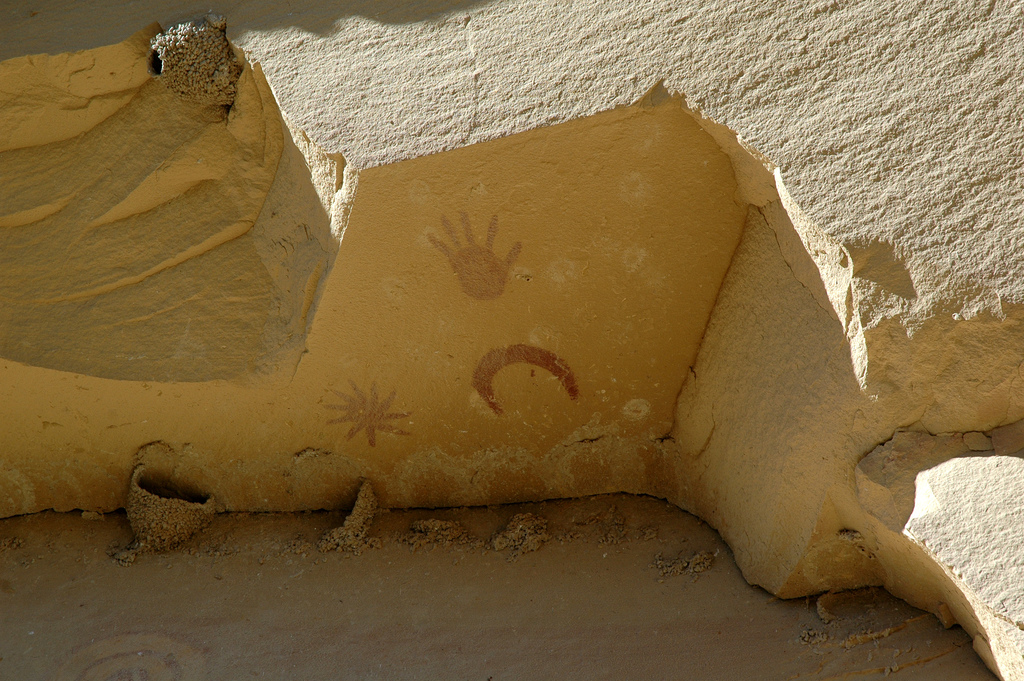
\includegraphics[width=\textwidth]{chapter_intro/plots/Chaco_canyon_pueblo_bonito_petroglyphs.jpg} 
   \caption{Chaco canyon petroglyphs show a hand, a moon and a bright celestial object. This could be SN1054 but it is ambiguous. (Source Wikipedia/ Photographer jamesdale10/ Creative Commons license)}
   \label{fig:sn1006_chaco}
\end{figure}


The supernova of 1572 has been reported by many astronomers. The most famous record, however, stems from the danish astronomer Tycho Brahe \citep{1602QB41.B73.......}. The supernova was observed from November 1572 and monitored till March 1574 when it faded from visibility. Figure \ref{fig:sn1572_tycho_chart} shows the original chart produced by Tycho Brahe which shows the supernova in the constellation of Cassiopeia. Nearly 400 years later \citet{1952Natur.170..364H} discovered the radio emissions from the remnant of the SN1572. 


32 years after the discovery of SN1572 Kepler and others observed SN1604 \citet{kepler1606} . The supernova remained visible for about 18 month. 

\begin{figure}[htbp] %  figure placement: here, top, bottom, or page
   \centering
   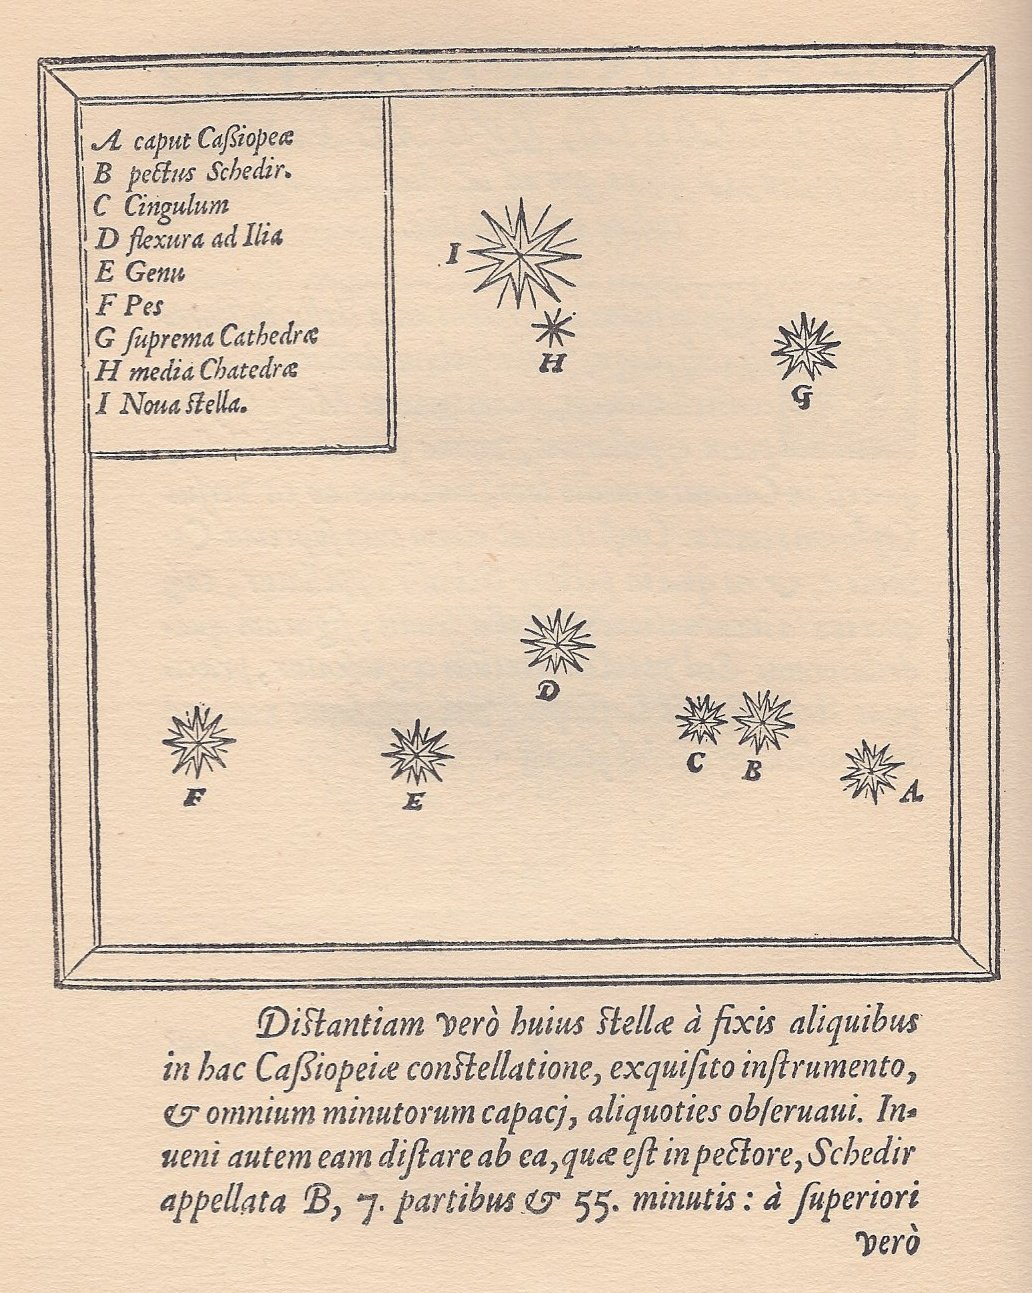
\includegraphics[width=0.7\textwidth]{chapter_intro/plots/Tycho_Cas_SN1572.jpg} 
   \caption{\textit{"I have indeed measured the distance of this star from some of the fixed stars in the constellation of Cassiopeia several times with an
exquisit (optical) instrument, which is capable of all the fine details of measurement. I have further detected that it
(the new star) is located 7 degrees and 55 minutes from the star at the breast of the Schedir designated by B."} translation kindly provided by Leonhard Kretzenbacher}
   \label{fig:sn1572_tycho_chart}
\end{figure}

All of the ancient supernovae were observed only by the naked eye. Even in an era of 10-meter telescopes the records of these explosions remain useful.

\section{Modern day supernova observations and surveys}
\label{sec:surveys}

The era of modern day supernova observations started with the discovery of \sn{1885}{}. \sn{1885}{} (also known as S Andromedae) was first spotted by Isaac Ward in Belfast in August of 1885 \citep{1885AN....112..360H} and was visible till February 1886. 
More than 50 years later \citet{1934PNAS...20..254B} coined the term supernova and established the difference between common novae and supernovae. \citet{1934PNAS...20..254B} also suggested that these luminous events are caused by the death of stars. 

In order to understand the phenomenon of the supernova better, Zwicky began a supernova search with the 18-inch Schmidt telescope . Zwicky found several supernovae which in turn inspired Minkowski to classify these supernovae by their spectra \citet{1941PASP...53..224M}. 
He categorized the 14 known objects into two categories. Those without hydrogen he called 'Type I', those with hydrogen he called 'Type II' (see section \ref{sec:sn_classification} for a more detailed description about classification).

With the advent of affordable computing in the 1960s the first computer controlled telescopes were build. The 24-inch telecope was built by the Northwestern University and was deployed in Corralitos Observatory in New Mexico \citep{1975PASP...87..565C}. This search lead the way in computer controlled discovery and many later surveys would employ a similar design.

The Cal\'{a}n/Tololo supernova survey \citep{1993AJ....106.2392H} ushered in the era of the modern automated supernova surveys in the 1990's. They provided a set of high-quality light curves and spectra of moderately distant $(0.01 < z < 0.01)$ supernovae.

The Leuschner Observatory Supernova Survey began in 1992 followed shortly by the Berkeley Automatic Imaging Telescope (BAIT). These searches resulted in 15 supernovae by 1994 \citep{1994AAS...185.7905V}. One of the most well known discoveries is \sn{1994}{D}. This supernovae was observed with the Hubble Space Telescope and resulted in an image that is widely used today.

Having started in 1988 the supernova cosmology project (henceforth SCP) is the longest running supernova search which is still active today. Their main sample for the famous paper \citep{1999ApJ...517..565P} used the CTIO 4m telescope for discovery and many other telescopes for follow-up.

The High-Z team used the CTIO 4m telescope for discovery and follow-up of supernovae \citep{1998ApJ...507...46S}. Independently to SCP they discovered the accelerated expansion of the universe \citep{1998AJ....116.1009R}.


The Lick Observatory Supernova Search (LOSS) using the Katzman Automatic Imaging Telescope (KAIT) is one of the most successful supernovae searches. By the year 2000 it had found 96 supernovae \citep{2001ASPC..246..121F}. 

After the turn of the millennium and following the discovery of the accelerated expansion of the universe a variety of groups started searching for supernovae and other transients. Among them were ``The Equation of State: SupErNovae trace Cosmic Expansion (ESSENCE)''-project \citep{2002AAS...201.7809G} and the Supernova Legacy Survey (SNLS) \citep{2003AAS...203.8209P}. Both these programs have either finished or are close to finishing. 

Specialised surveys like the Nearby Supernova Factory \citep{2002SPIE.4836...61A} and the Higher-z survey \citep{2004ApJ...613..200S} focused on a certain redshift range to obtain data on supernovae.

In recent years a multitude of large sky surveys has started (or are just about to). Some of these focus exclusively on transients and supernovae \citep[e.g. PTF;][]{2009PASP..121.1334R}, whereas others like PanSTARRS \citep{2004SPIE.5489...11K} and SkyMapper \citep{2007PASA...24....1K} have a transient/supernova component. 
Upcoming surveys like the LSST \cite{2006AAS...209.8604P} and the space-based GAIA mission \cite{2001A&A...369..339P} will provide unprecedented detail about current supernovae as well finding several new classes of transients.

In addition to the search in the optical new high-energy instruments like BATSE surveyed the sky from the beginning of the 1990's in \gammaray s. \citet{1992Natur.355..143M} showed that \grb s due to their isotropic distribution are events at cosmological distances rather than coming from our own Galaxy. 

The Beppo-SAX satellite played a crucial role in resolving the origins of \grb s. The data from this mission was used to establish the connection between some \grb s and supernovae, the most famous example being GRB980425/\sn{1998}{bw} \citep{1998Natur.395..670G}.

Among other discoveries the Hete-2 mission established a new class of transients called \xray-flashes. These new objects are thought to be similar to  \grb s in the physical nature but much less energetic \citep{2004ApJ...601L.119Z}.  

It was followed by the SWIFT telescope which provides, in addition to the \gammaray-detector, an X-Ray telescope and UV/Optical telescope. It has been very successful at finding \grb s and providing targets for follow-up.

Almost all of the information about the universe we have deduced from observations of electro-magnetic waves. There are different physical phenomena which are much harder to observe than the electro-magnetic spectrum.

Gravitational waves, predicted by the theory of general relativity  \cite{1918SPAW.......154E}, might provide us with another insight into supernovae. The most advanced detector today \cite[LIGO][]{1992Sci...256..325A} has up till now not unambiguously detected gravitational waves. The sensitivity for this instrument is probably not low enough to detect these waves. Future instrumentation, like the impressive LISA-project \citep{1994ESAJ...18..219J}, are sensitive enough to detect the predicted gravitational waves. In the supernova field LISA might give us an estimate on the number of in-spiralling white dwarfs, which are suggested as progenitors of \sneia.

\citet{1987PhRvL..58.1494B,1987PhRvL..58.1490H,Alekseev:1988gp} reported on neutrino detections from the very nearby supernova SN1987A. This was the first and last time that neutrino emission from a supernova was measured. New more sensitive detectors like ICECUBE \citep{2008ICRC....4..835K} will hopefully enable us to do neutrino observations of more distant events.

For now the optical observations of supernovae provide the bulk of observations of these transients. Hopefully future instruments and capabilities will give us panchromatic observations as well as measurements from gravitational waves and particle fluxes. 
This will hopefully help to unlock more of the secrets of these still mysterious supernovae.

\section{Observational Properties of Supernovae}

\subsection{Supernova classification}
\label{sec:sn_classification}

The classification of supernovae started in the 1941 when Minkowski realized that there seem to be two main types \citep{1941PASP...53..224M}. Those containing a hydrogen line (6563 \AA) he called Type II supernovae and those showing no hydrogen he called Type I supernovae.  

\begin{figure}[htb] %  figure placement: here, top, bottom, or page
   \centering
   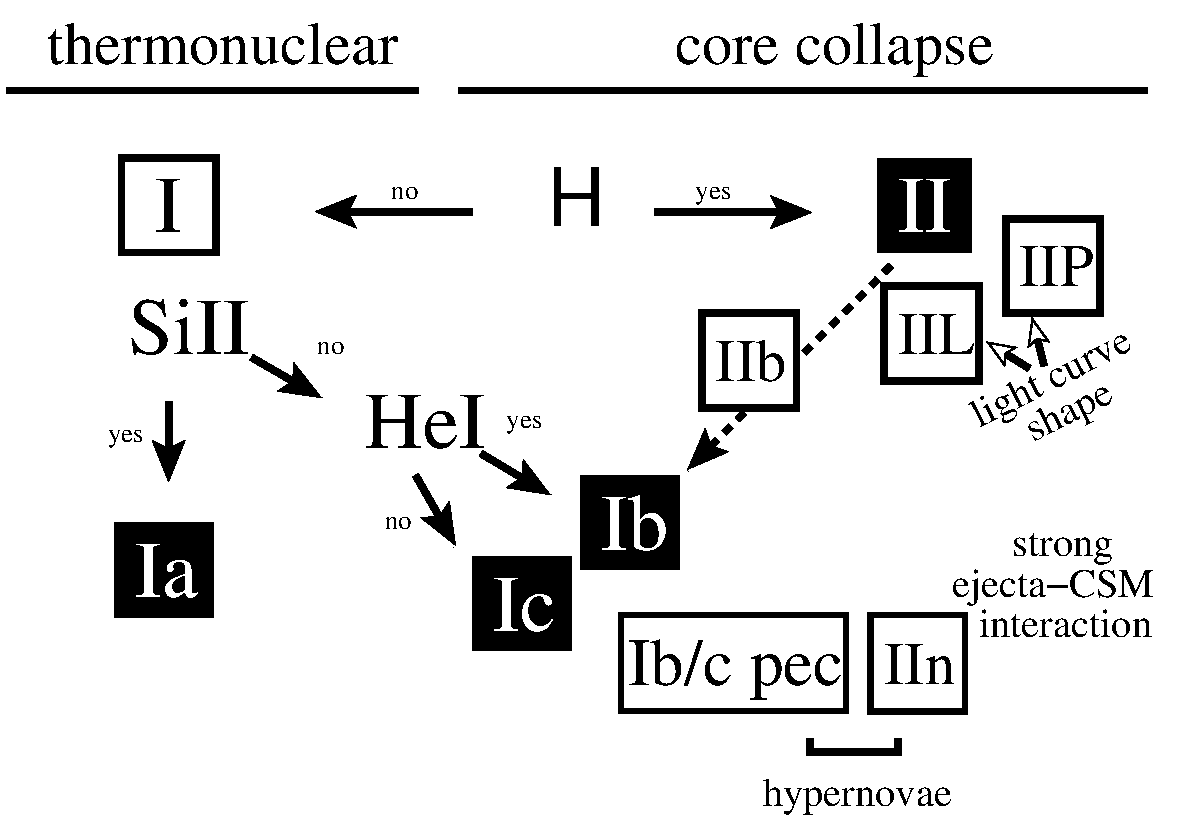
\includegraphics[width=.7\textwidth]{chapter_intro/plots/sn_classification.pdf} 
   \caption{}
   \label{fig:sn_classification}
\end{figure}

This basic classification has remained to this day, however the two main classes branched into several subclasses.
During the 1980s the community discovered that most \sneia\ showed a broad Si II line at 6130 \AA. There was, however, a distinct subclass of objects that lacked this feature. These Silicon-less objects were then subclassed further into objects that showed helium -- now known as Type Ib --  and those that did not were called Type Ic \citep[see spectra in Figure \ref{fig:sn_classification};]{1987ApJ...317..355H, 1986ApJ...306L..77G}. The classical Type I supernova was renamed to Type Ia. 

\begin{figure}[htb] %  figure placement: here, top, bottom, or page
   \centering
   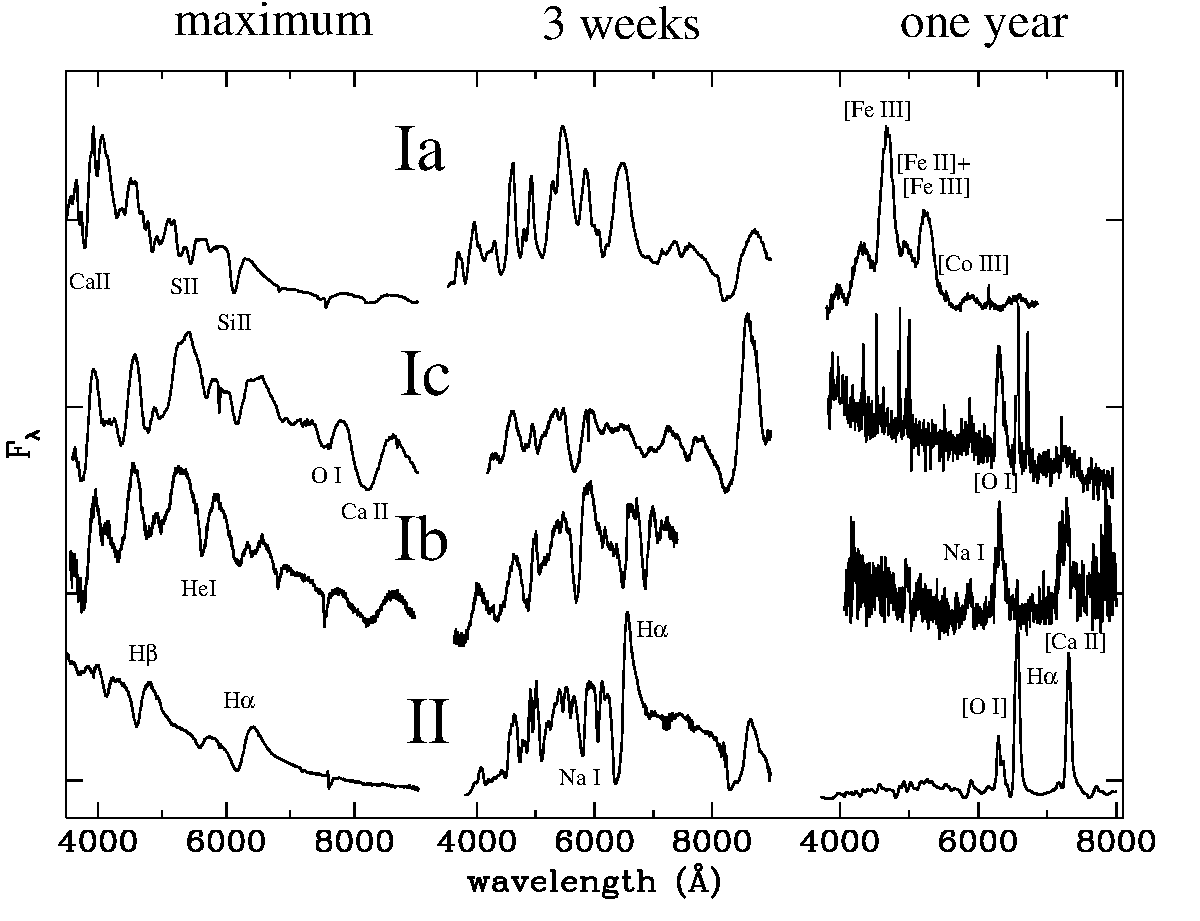
\includegraphics[width=0.7\textwidth]{chapter_intro/plots/sn_class_spectra.pdf} 
   \caption{example caption}
   \label{fig:sn_class_spectra}
\end{figure}

%This classification only uses static spectral features. In recent years, however, there has been a push towards also using the lightcurve and spectral evolution as classification parameters. \citet{2005ApJ...623.1011B} provide an overview of this subclassing of \sneia\ and suggest that there are two distinct subclasses of \sneia. As a parameter for this further partitioning they use the velocity measured from the Si II feature at 6130 \AA. Those with a relatively fast decline in this radial velocity they call \hvg\ (high velocity gradient) those with a slow decline rate are named \lvg\ (low velocity gradient). 

\sneia\ show a low intrinsic scatter in peak luminosity. Only in the past two decades have we been able to explore the finer details of the \sneia-class.
Most objects have a small brightness scatter and are referred to as ``Branch''-normal \citep{1993AJ....106.2383B}. 
There however seem to be two distinct subclasses with extreme luminosities. The overluminous class we call 91T\,s after the bright supernova \sn{1991}{T} \citet{1992AJ....103.1632P, 1994ApJ...434L..19S} and the faint 91bg\,s named after the faint \sn{1991}{bg}\ \citep{1992AJ....104.1543F}.  As a further characteristic the community uses the velocity inferred from the Si II feature at 6130 \AA.
Faint supernovae are fast decliners both in velocity as well as luminosity \citet{2005ApJ...623.1011B}. The bright supernovae do not seem to have such a preference. 
A third subclass named after \sn{2002}{cx}\ \citep{2003PASP..115..453L} seems to contradict this theme. They decline slow and are faint. This subclass also shares spectral traits with the overluminous 91T\,s.

\citet{2011MNRAS.412.1441L} have tried to measure the fraction of these different subclasses from the Lick Observatory Supernova Search (LOSS). Figure \ref{fig:ia_fracs} shows the fraction of the different subclasses that would be expected from a purely magnitude limited search. 

\begin{figure}[htbp] %  figure placement: here, top, bottom, or page
   \centering
   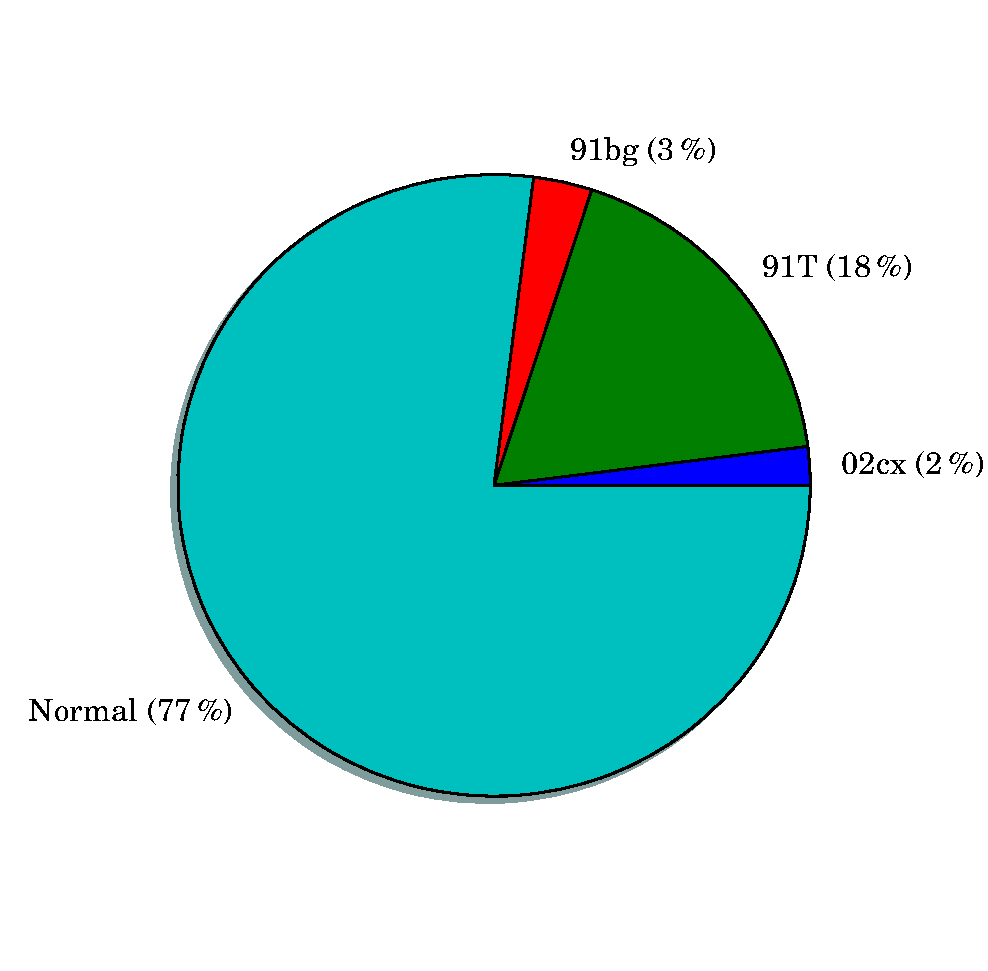
\includegraphics[width=0.7\textwidth, trim=0 2.5cm 0 0cm]{chapter_intro/plots/plot_ia_fracs.pdf} 
   \caption{Estimated fractions for different \snia-classes for a purely magnitude limited search. Adapted from \citet{2011MNRAS.412.1441L}}
   \label{fig:ia_fracs}
\end{figure}

In summary, although there are several different subclasses, the \snia\ as a class itself is relatively homogenous when compared to the different \sneii.

\begin{figure}[htbp] %  figure placement: here, top, bottom, or page
   \centering
   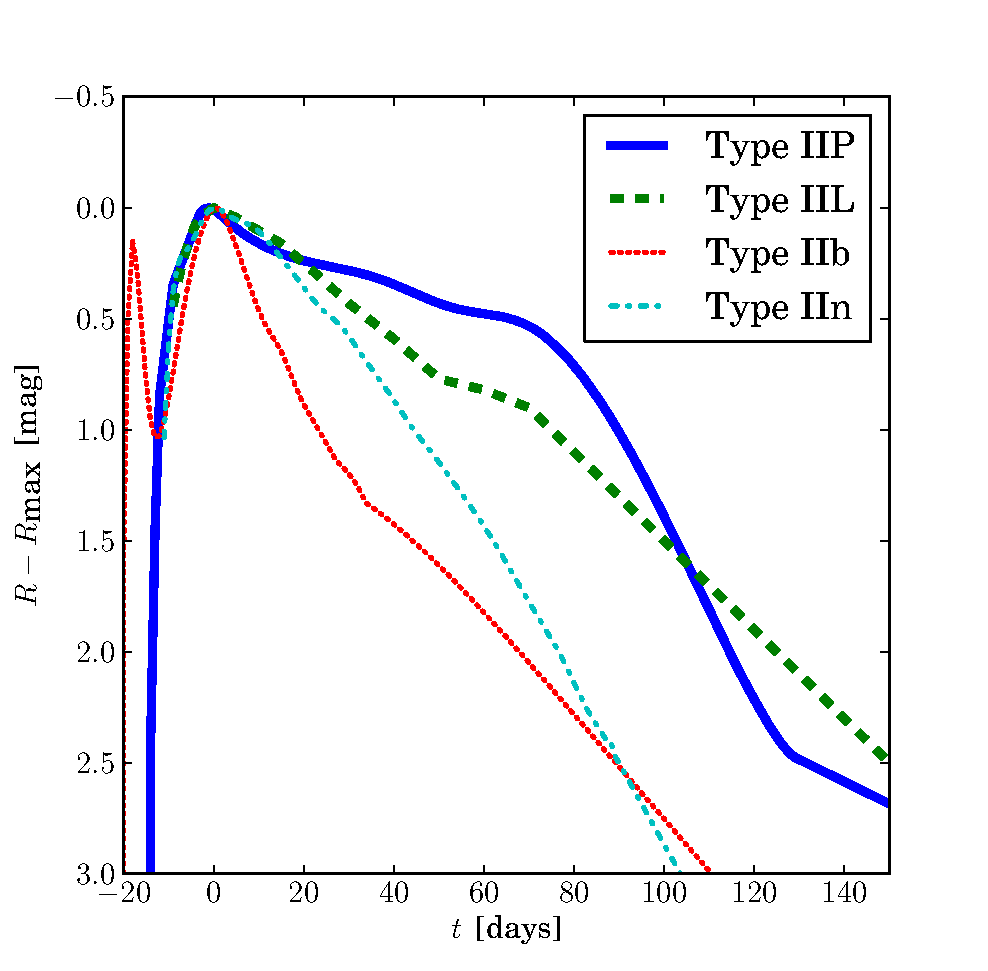
\includegraphics[width=0.7\textwidth]{chapter_intro/plots/plot_li11_lc_type2.pdf} 
   \caption{Lightcurve data taken from \citet{2011MNRAS.412.1441L} templates. The time is relative to maximum light and the magnitude is the difference between maximum  }
   \label{fig:snii_lc}
\end{figure}

\sneii\ span large ranges in observable parameters. We can divide the main class into four main subclasses. Type II Plateau Supernovae \citep[henceforth \sniip;][]{1979A&A....72..287B} have a relatively flat light curve after an initial maximum (see Figure \ref{fig:snii_lc}). In contrast the Type II Linear Supernovae \citep[henceforth \sniil;][]{1990MNRAS.244..269S} have a rapid linear decline after the maximum. The third subclass is the narrow-lined Type II Supernova (henceforth \sniin) which is characterized by narrow emission lines, which are thought to come from interaction with the \csm. 
Finally the Type IIb supernovae (henceforth \sniib) show strong hydrogen lines in their early spectrum, but evolve to become spectroscopically to be more like Type Ib supernovae with no hydrogen lines but strong Silicon and Helium lines. An interesting feature is the second maximum observed in the \sniib \sn{1993}{J} (Figure \ref{fig:snii_lc}). It is believed that many more \sniib s exhibit this feature but are not detected early enough \citep[this feature has also been seen in SN2008D a  \snib][]{2008Natur.453..469S, 2009ApJ...702..226M}. 

Figure \ref{fig:ii_fracs} shows the estimated fractions of the different \sneii\ that would be expected from a purely magnitude limited survey.

\begin{figure}[htbp] %  figure placement: here, top, bottom, or page
   \centering
   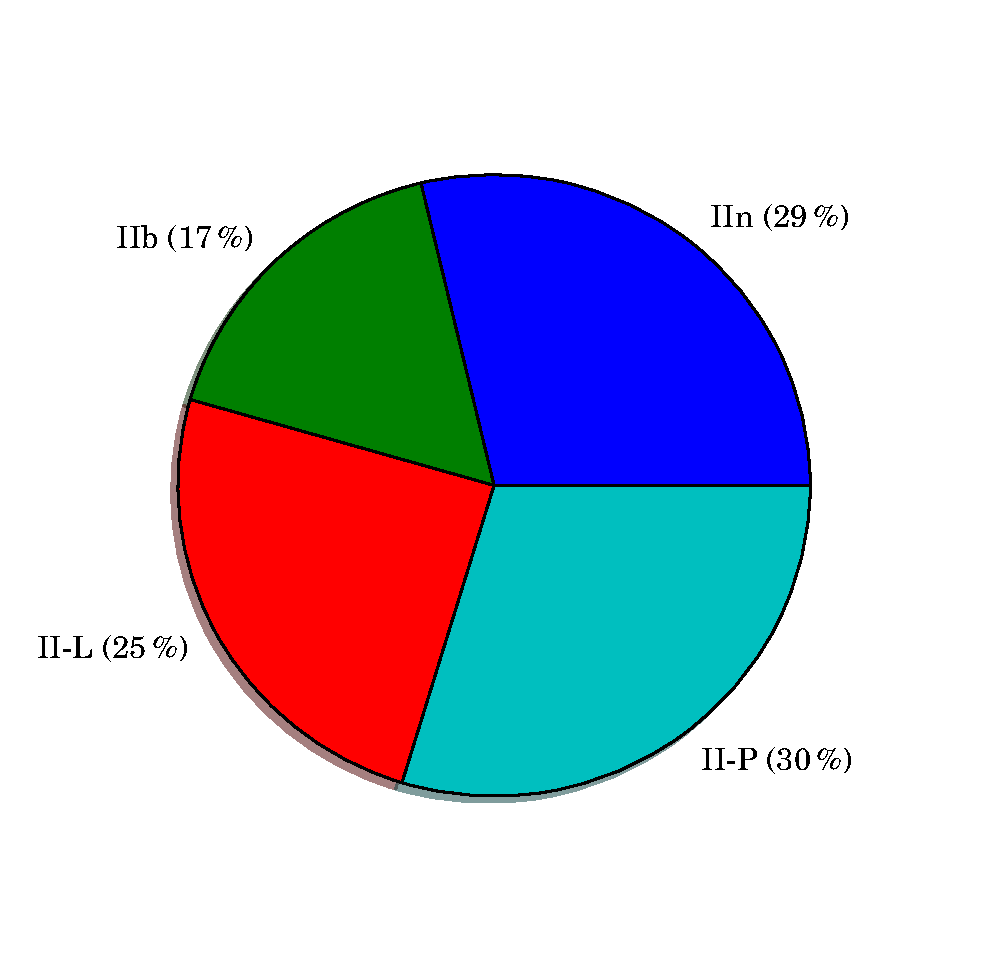
\includegraphics[width=0.7\textwidth, trim=0 2.5cm 0 0cm]{chapter_intro/plots/plot_ii_fracs.pdf} 
   \caption{Estimated fractions for different \snii-classes for a purely magnitude limited search. Adapted from \citet{2011MNRAS.412.1441L}}
   \label{fig:ii_fracs}
\end{figure}


Unlike the \sneia\ there are numerous intermediate objects among these three basic classes and some peculiar objects.


For a more comprehensive review of the classification of supernovae the reader should consult \citet{2003LNP...598...21T} and \citet{2007AIPC..937..187T}.

\subsection{Supernova rates}
\label{sec:sn_rates}
The observed supernova frequency carries important information about the underlying progenitor population. In this section we will concentrate more on \sneia-rates but will mention \sneii\ and \sneibc where applicable.

\citet{1938ApJ....88..529Z} was the first work that tried to measure the supernova rate. By monitoring a large number of fields monthly, they arrived at a supernova rate by merely dividing the number of supernova detection by the number of monitoring time and galaxies. This crude method resulted in a rate of one supernova per six centuries. 

Over time many improvements were made to this first method. The rate was divided by galaxy morphological class as well as different supernova types. To normalise these quantities were then defined by the supernova rate as number of events per century per $10^{10}$\,\lsun\ \citep[e.g.][]{1991ARA&A..29..363V,1994ApJS...92..487T}. 

In recent years, however, rate measurements have been in relation to star formation rather than galaxy luminosity (\sn\ per century per $10^{10}$\,\msun).  The community \citep[e.g.][]{2005A&A...433..807M} have switched to the use of infrared photometry for the galaxy as it is thought to better represent star-formation rate then B-Band photometry \citep{2003A&A...410...83H} which had been used previously. 
\begin{figure}[htbp] %  figure placement: here, top, bottom, or page
   \centering
   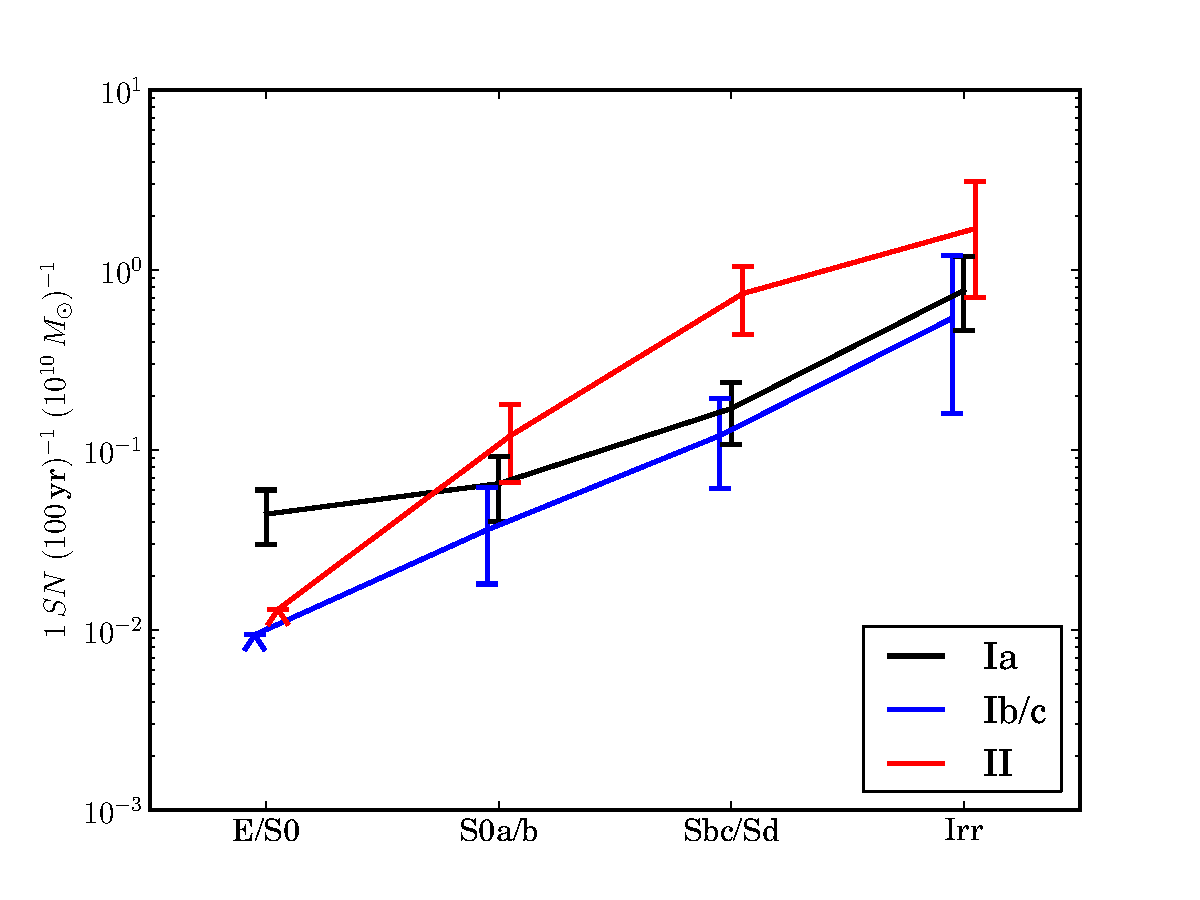
\includegraphics[width=\textwidth]{chapter_intro/plots/snrates_mannucci05.pdf} 
   \caption{The plot shows the estimated supernova rate per unit mass in different galaxy morphologies \citep{2005A&A...433..807M}. There have been no detections of \sneibc\ and \sneii\ in old elliptical galaxies which suggests that these types only occur in galaxies with recent star-formation.}
   \label{fig:snrates_mannucci05}
\end{figure}

Figure \ref{fig:snrates_mannucci05} clearly shows that there is a strong connection between morphology and supernova rates. This suggest that \sneii\ and \sneibc\ come from populations with recent star formation, which implies massive stars as progenitor. \sneia\ occur both in old elliptical galaxies and young spirals. It seems the progenitors occur in both of these environments. This could hint that there are two main progenitor types one which occur soon after star-formation, whereas others take a long time between formation and explosion. The progenitors of \sneia\ are a highly debated topic (see Section \ref{sec:snia_progenitors}).

To address this issue several groups have tried to measure a \sneia-rate that is completely independent of galaxy morphology \citep[e.g.][]{2006MNRAS.370..773M, 2010ApJ...722.1879M}. This so called, delay time distribution (\dtd), measures the supernova rate over time following a brief outburst of star formation.
This technique requires a detailed knowledge of the star-formation history of these systems. Several new techniques are emerging that try to circumvent the intrinsically difficult task of determining star-formation for individual \sneia\ host galaxies \citep{2010MNRAS.407.1314M, 2010arXiv1010.5786B, 2008PASJ...60.1327T, 2010ApJ...722.1879M}.

Supernova rates and \dtd s are a great tool to constrain progenitors. New upcoming surveys will provide an abundance of supernovae and measurements of their environments.

\subsection{Light curves} 
\label{sec:intro_lc}
Light curves give important insights into the physical reactions occurring during the evolution of the supernova. \cite{1982ApJ...253..785A} for example deduced from the light-curve shape that Type I supernova are eventually powered by the decaying \Co. 


\begin{figure}[htb] %  figure placement: here, top, bottom, or page
   \centering
   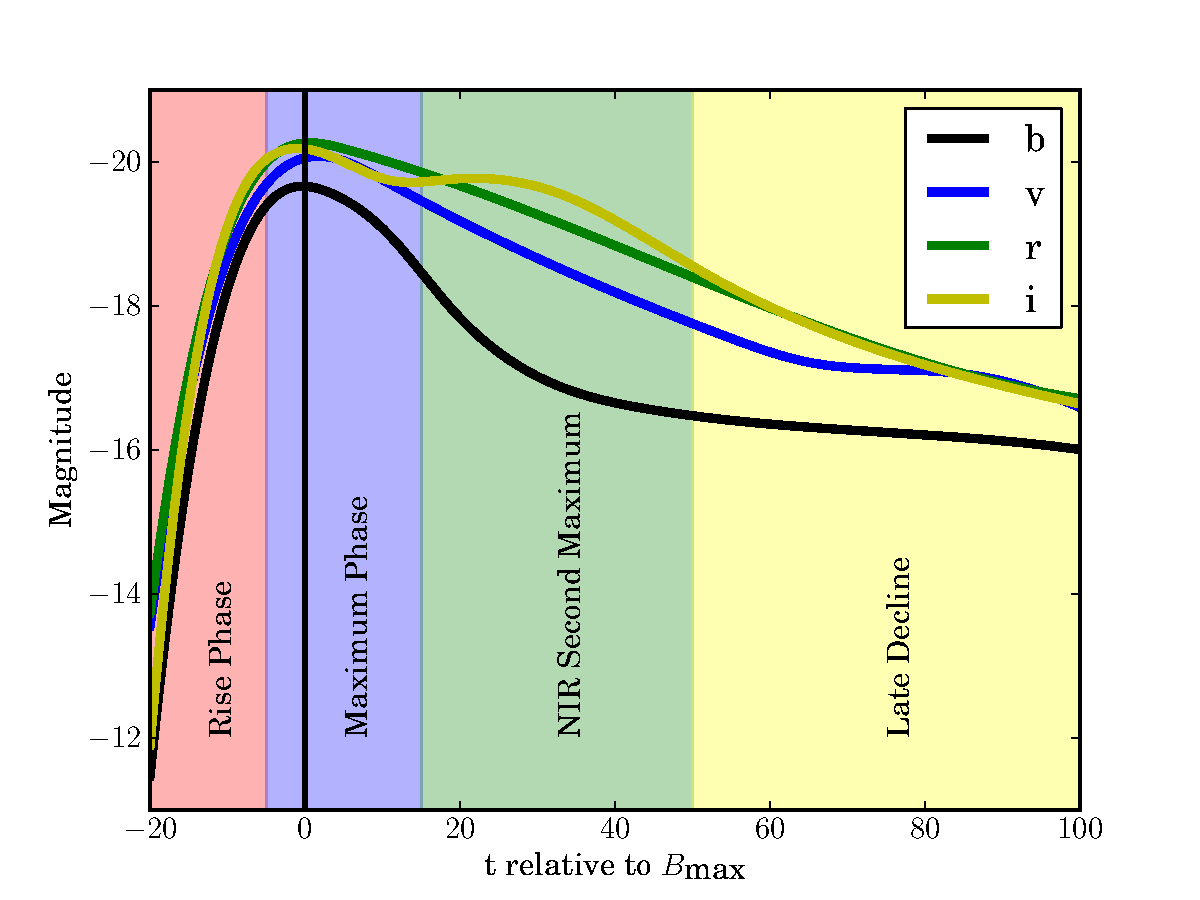
\includegraphics[width=\textwidth]{chapter_intro/plots/lightcurve_2002bo.pdf} 
   \caption{Lightcurves of SN 2002bo (data from ??)}
   \label{fig:lightcurve_2002bo}
\end{figure}

For \sneia\ the light curve can be divided in four different phases (see Figure \ref{fig:lightcurve_2002bo}). In the first phase the \sneia\  rises to the maximum brightness. Although only a small fraction of \sneia\ have been observed in that phase, one can determine the time of the explosion by approximating the very early phase of a \sneia\ with an expanding fireball. The luminosity of the fireball is 
\[L\propto v^2 (t+t_\textrm{r})^2 T\,,\]
where v is the photospheric velocity, T is the temperature of the fireball, t is the time relative to the maximum and $t_\textrm{r}$ is the rise time. A rise time of 19.5 days \citep{1999AJ....118.2675R} seems to fit most \sneia. 

The rise is very steep and the brightness increases by a factor of $\approx 1.5$ per day until 10 days before maximum. 

The \snia\ reaches the maximum first in the \nir\ roughly 5 days before the maximum in the B-Band \citep{2000MNRAS.314..782M}. 
During the pre-maximum phase the color stays fairly constant at B-V=0.1, but changes non-monotonically to B-V=1.1 30 days after maximum. 

The \snia\ starts to fade but  a second maximum is observed in the \nir\ \citep{2008ApJ...689..377W}.  \citet{2006ApJ...649..939K} has succesfully explained this by fluorescence of iron-peak elements in the \nir. 

At roughly 600 days after maximum the light curve begins ???? 1991t had a foreground dust??? (how late do light curves go; a comment would be nice here brian ;-) ) 

Arguably the most important use of light curves is their application in normalizing \sneia\ to standard candles (see Figure \ref{fig:normalized_lightcurve}). \citet[][]{1993ApJ...413L.105P} plotted the magnitude at maximum in different filters against the decline of the B-Band magnitude after 15 days (\dmb).  They found a strong linear relation with a very high correlation coefficient ($>$ 0.9). Dust extinction in the host is one of the major systematic problems and remains so to this day. 

\cite{1995ApJ...438L..17R} refined the method by using a linear estimation algorithm. This method would deliver a distance modulus by finding the offset between a template and the supernova lightcurve. They calibrated this method against a set of \sneia\ with known distances. 
Light curve fitting tools are still in active development \cite[e.g.][]{2007ApJ...659..122J, 2007A&A...466...11G}.

For description of lightcurves of \sneii\ please refer back to section \ref{sec:sn_classification}.


\subsection{Spectra} 
\label{sec:intro_sn_spectra}
Spectra are much more detailed measurements of Supernovae than just lightcurves. They are however, observationally much more expensive. 

For all classes supernova spectra can be divided in two phases: the photospheric phase and the nebular phase.
In the photospheric phase, the spectrum can be very well approximated by a dense optically thick core which has a black-body radiating surface with an optically thin expanding ejecta above. Photons is often negligible in the ejecta. The ejecta rather reprocesses the radiation field coming from the central photosphere. 
In the case of \sneia\ the core consists mainly of decaying \Ni\ which produces the energy for the radiating photosphere. For \sneii\ the core mainly consists of ionized hydrogen.

As the supernova expands the photosphere recedes further into the core and the optically thin layer grows larger and larger. Once sufficiently expanded the entire SN ejecta becomes optically thin, which is known as the nebular phase. This phase is dominated by strong emission peaks and no continuum. 


\subsubsection{SNe Ia spectra}
\label{sec:intro_sneia_spectra}
\sneia\ spectra help us understand the physical processes in the thermonuclear explosion. 
Shortly after the explosion the ejecta is in homologous expansion.
The observed spectra are characterized by an underlying continuum - emitted from the photosphere -- and absorption features from the ejecta material above the photosphere. 
As time passes the photosphere recedes into the remnant and deeper layers of the exploded white dwarf become spectroscopically visible. Synthetic modelling of spectra is an important component to understanding \sneia\ and will be discussed in detail in Chapter \ref{chap:dalek}.

This time-variability in the spectra is used to conduct tomography on \sneia\ \citep{2005MNRAS.360.1231S, 2009MNRAS.399.1238H}.

Similar to light-curves the spectra have different phases. We will use the ``normal''-\snia\ \sn{2003}{du} to demonstrate the spectral evolution \citep{2011MNRAS.410.1725T}. 

\paragraph{Pre-Maximum Phase}
In the pre-maximum phase the spectrum shows very high velocities (up to 18 000 \kms). There is a relatively well defined pseudo-continuum with strong \pcygni-profiles of \ime s and \ige s (see Figure \ref{fig:sn2003du_m10.9}). These \ige s are primordial as the burning in the outer layers (visible at these early times) is incomplete and does not produce these elements. 


\begin{figure}[htbp] %  figure placement: here, top, bottom, or page
   \centering
   \subfloat[SN 2003du 10 days before maximum light. The \pcygni-profiles of Silicon are clearly visible]{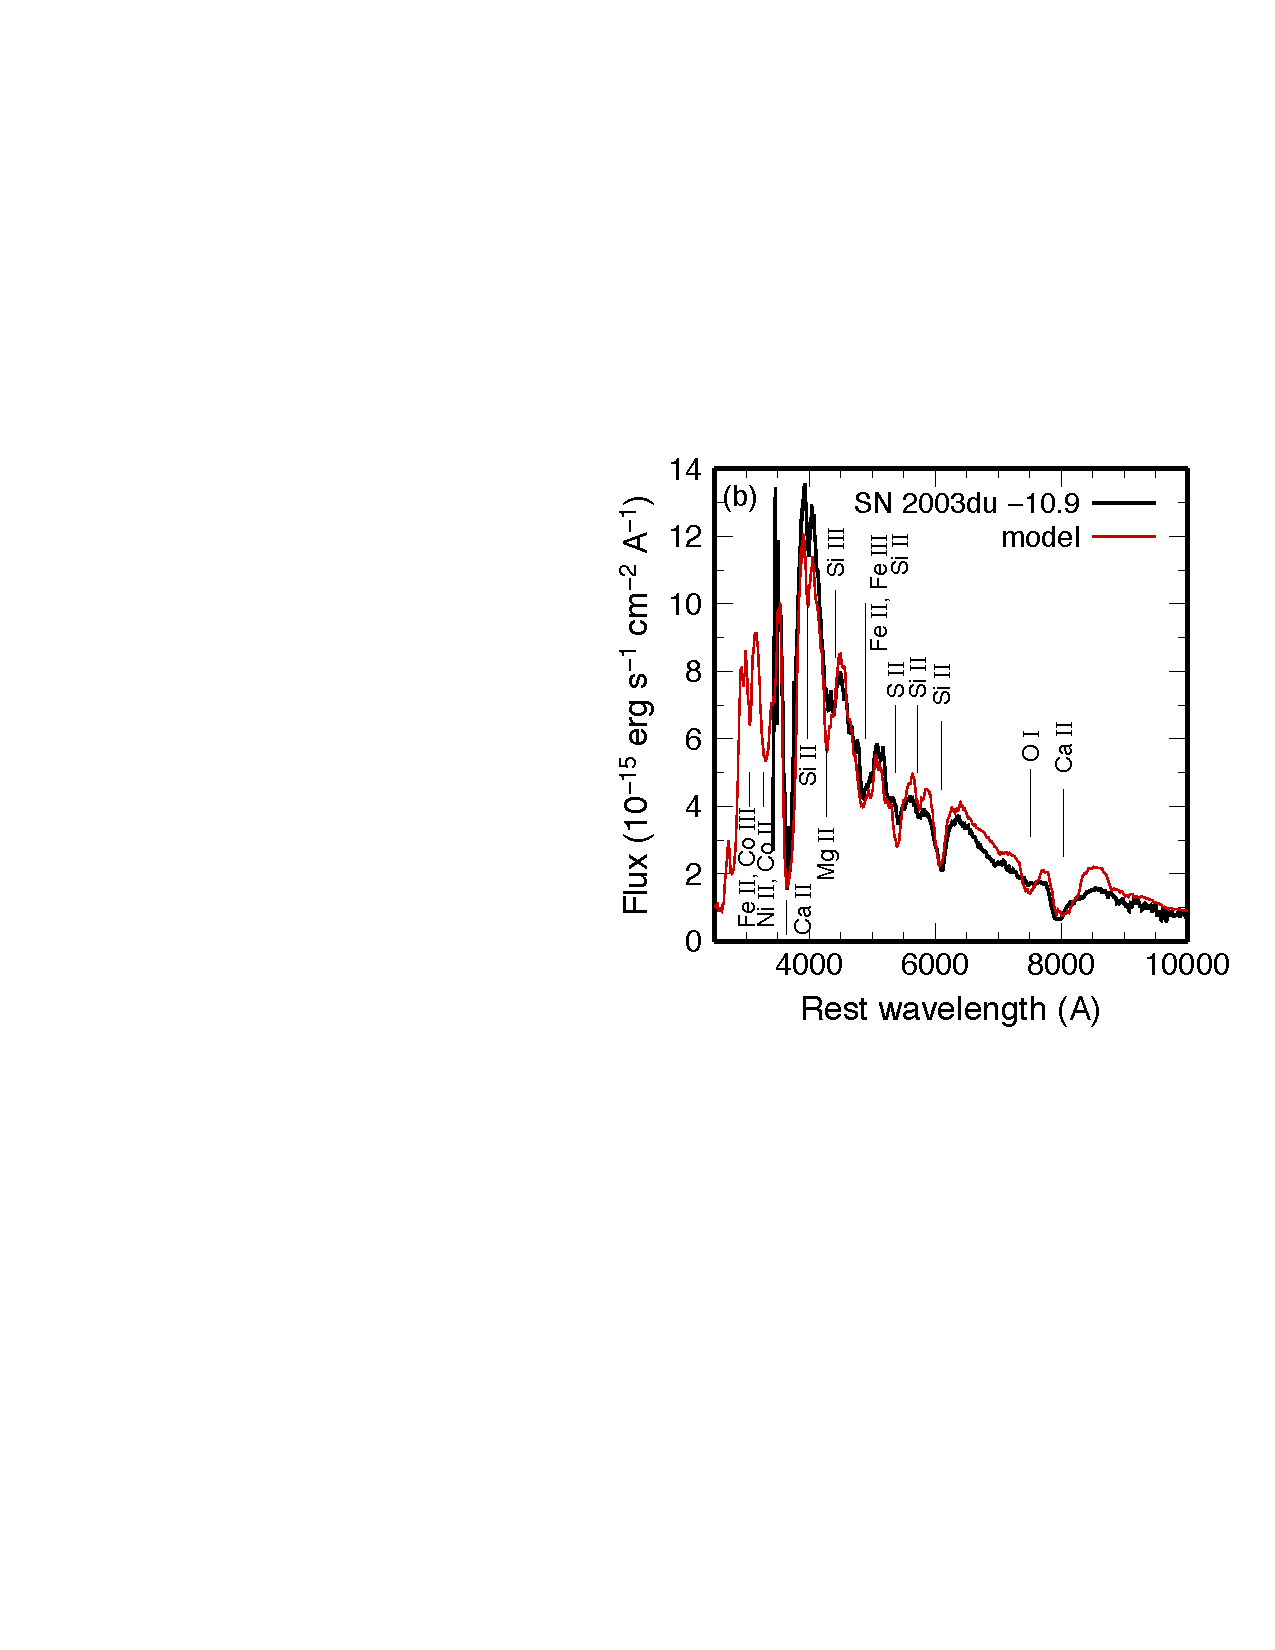
\includegraphics[width=0.45\textwidth]{chapter_intro/plots/sn2003du_t-10.pdf}}%
    \subfloat[SN2003du spectrum at maximum light. The light in the UV is being supressed and fluoresced into the red part of the spectrum.]{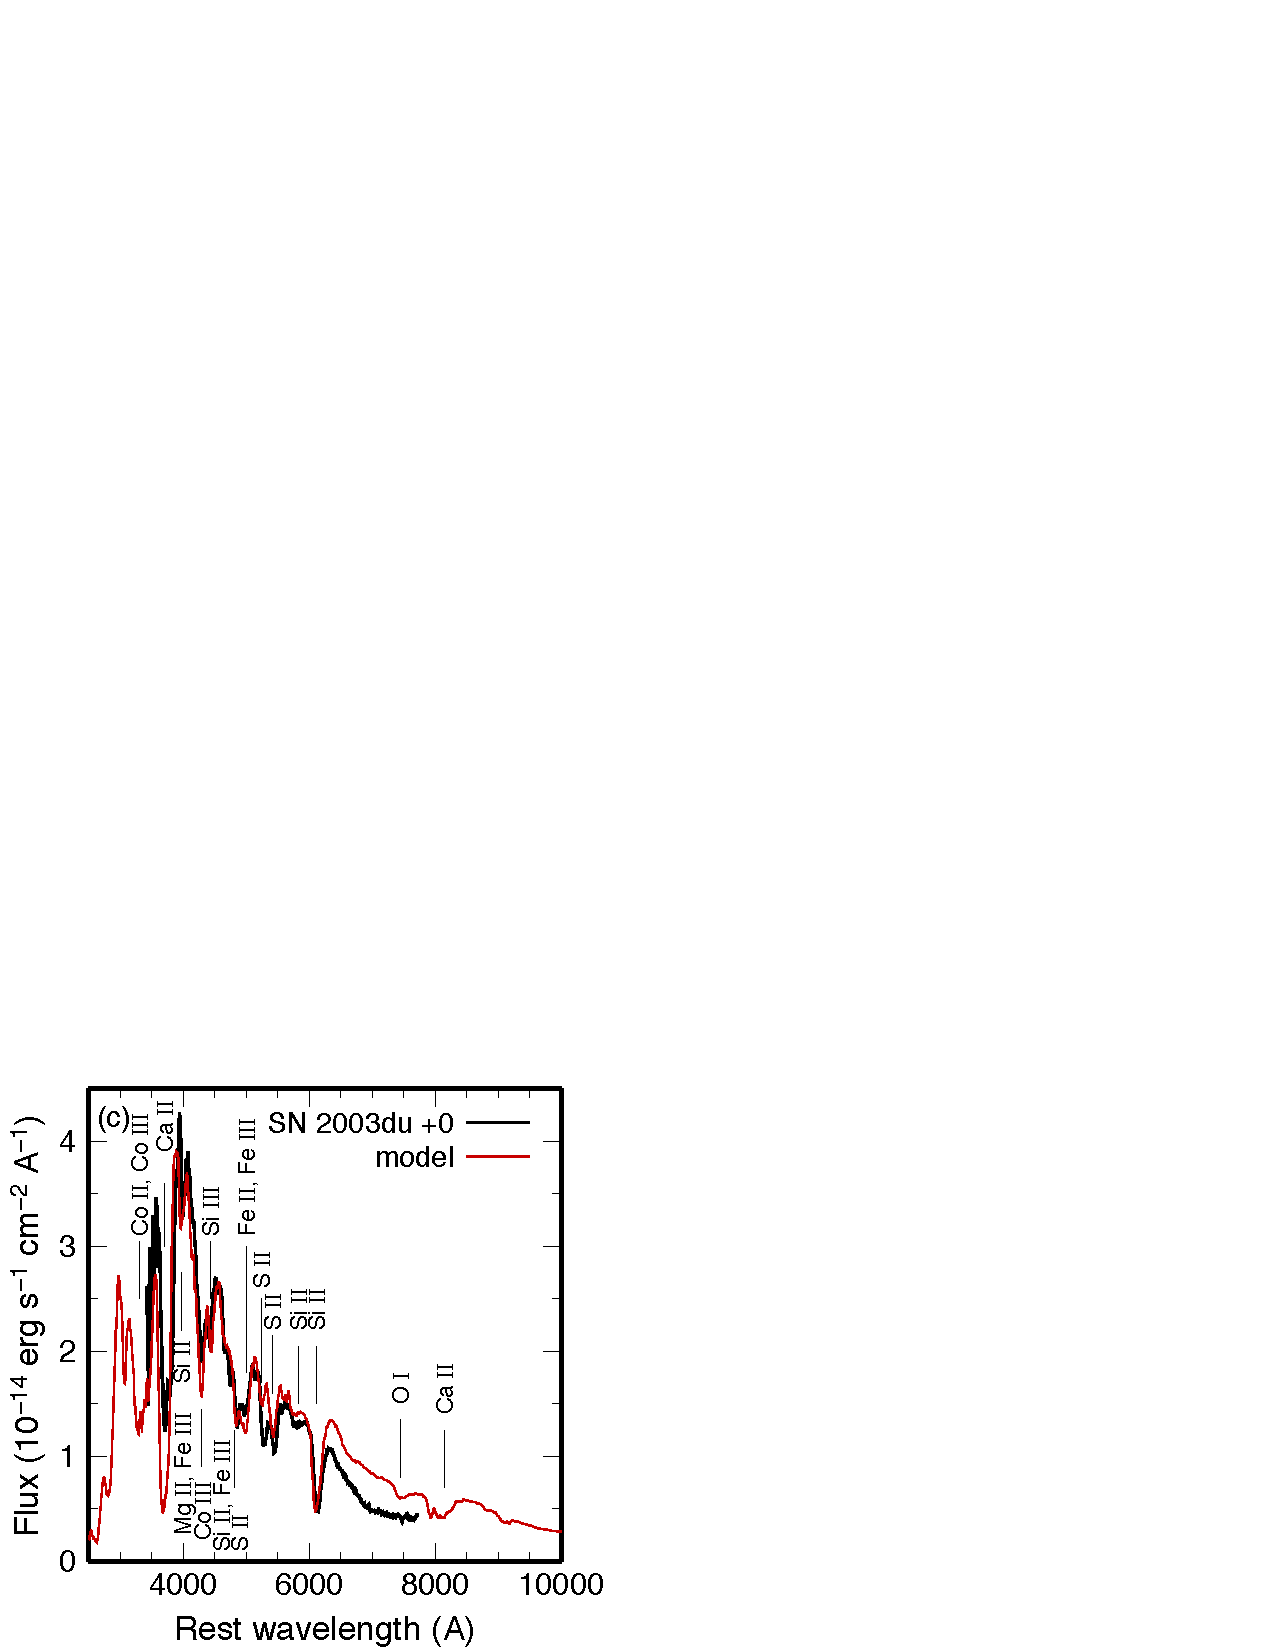
\includegraphics[width=0.45\textwidth]{chapter_intro/plots/sn2003du_t0.pdf}}%
   \caption{Premaximum evolution of \sn{2003}{du} spectra from \cite{2011MNRAS.410.1725T}.}
   \label{fig:sn2003du_premax}
\end{figure}

The \ion{Ca}{2} line is very prominent in the blue and often shows extremely high velocities at early times (in \sn{2003}{du} $v \approx 25000$\,\kms). There have been multiple suggestion for the cause of this unusual velocity, including interaction with Calcium in the \ism\ or high-velocity ejecta blobs \citep{1999ApJ...525..881H,2004ApJ...607..391G,2004ApJ...601.1019T,2005ApJ...623L..37M,2006ApJ...636..400Q,2006ApJ...645..470T,2007A&A...471..527G}.
There is a strong \ion{Mg}{2} feature at 4200\,\AA\ which is contaminated by several iron lines. Silicon and Sulphur both have strong features 5640\,\AA (\ion{S}{2}) and at 6355\,\AA (\ion{Si}{2}). The strong Silicon feature is the trademark for \sneia.

It is believed that in these early phases one should be able to see Carbon and Oxygen from the unburned outer layers. There is the \ion{C}{2}-feature at 6578\,\AA\ but it is normally very weak (if visible at all). The Oxygen triple feature at 7774\,\AA\ is also seldom very strong.

\paragraph{Maximum Phase} As the supernova rises to the peak luminosity a large fraction of iron group elements (especially \Ni) is suppressing flux in the UV and reemitting it in the optical (see Figure \ref{fig:sn2003du_premax}). The silicon lines become narrower as the photosphere reaches material deeper in the remnant. The ratio of the Silicon lines \ion{Si}{2} 5972\,\AA\ and \ion{Si}{2} 6355\,\AA\ is a good indicator for temperature \citep{1995ApJ...455L.147N}. 


\paragraph{Post-Maximum phase}
The contribution from iron-group elements is still rising, while the photospheric velocity has decreased to less than 10000\,\kms (see Figure \ref{fig:sn2003du_t+17}). The strong Calcium feature at 4000\,\AA\ is starting to disappear. 

\begin{figure}[htbp] %  figure placement: here, top, bottom, or page
   \centering
    \subfloat[SN 2003du 17 days past maximum light. The contribution of \ige is still rising.]{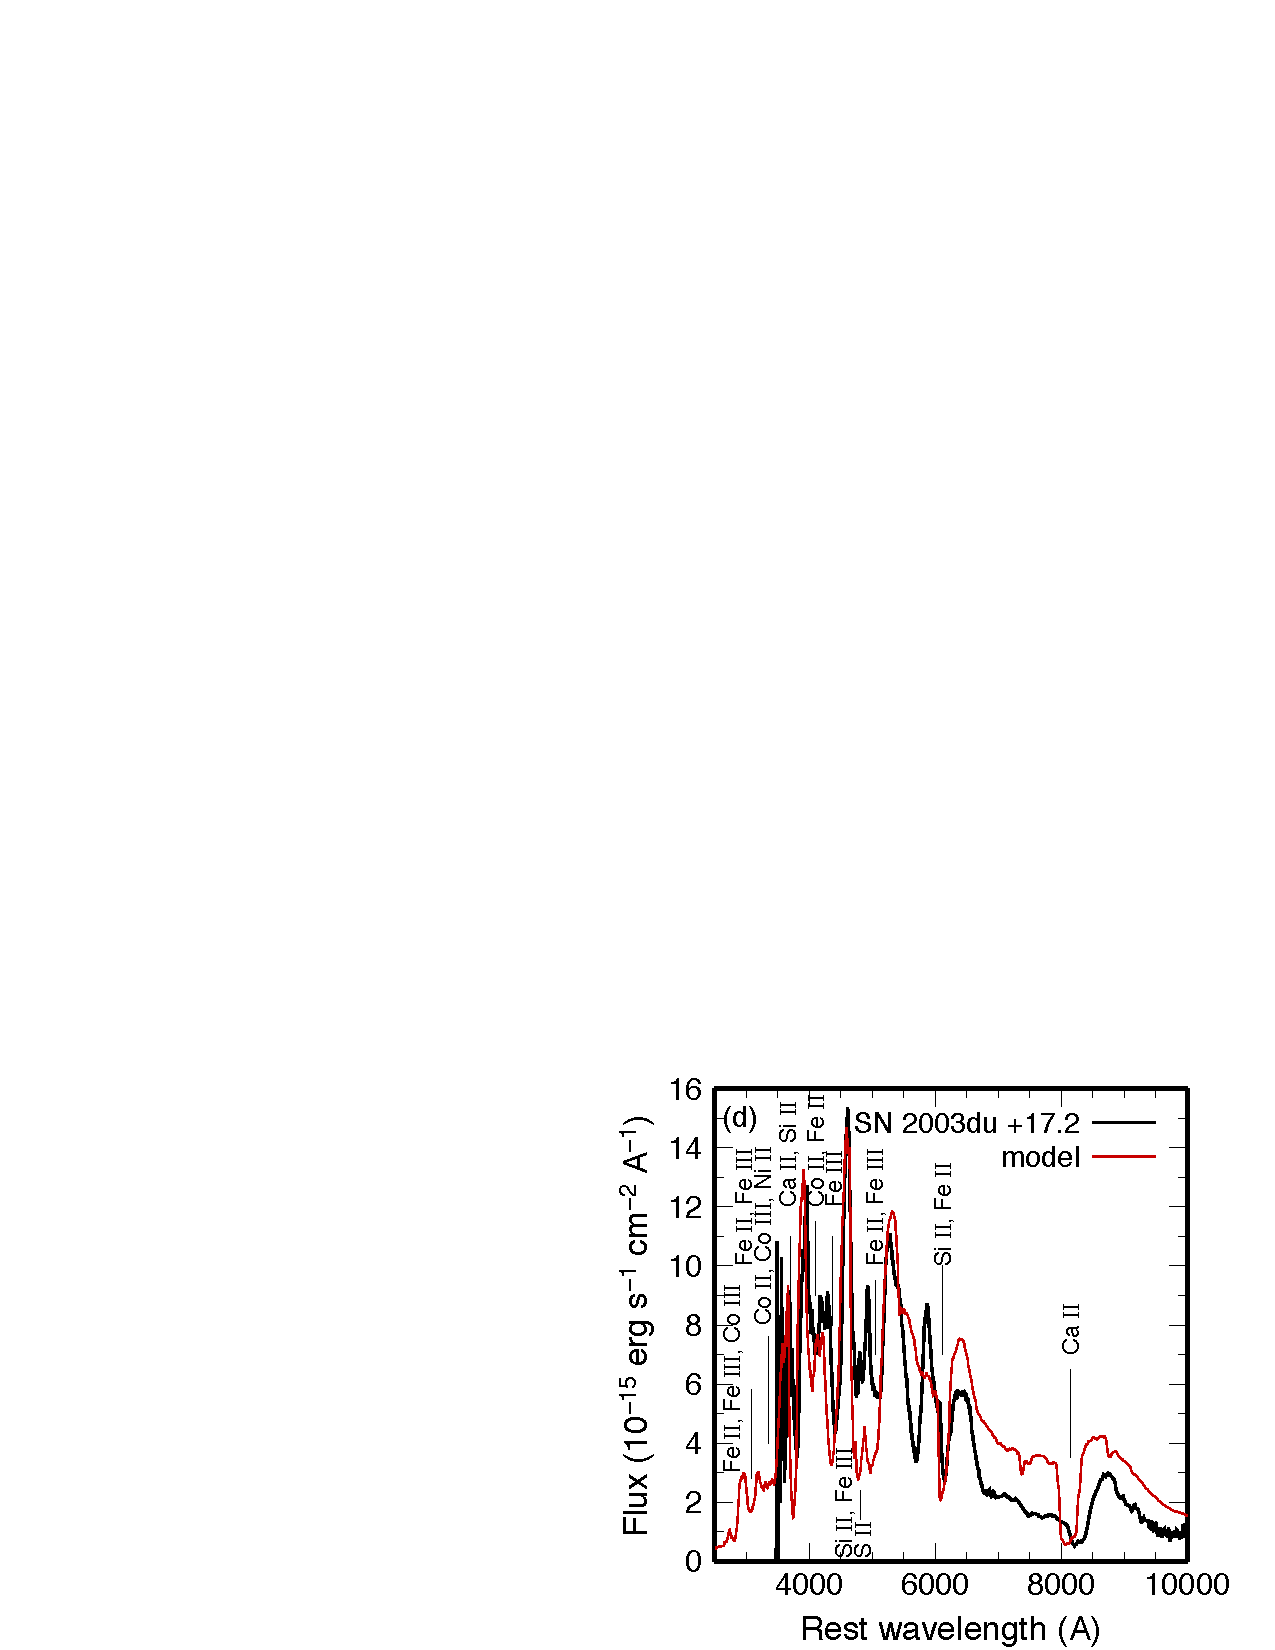
\includegraphics[width=0.45\textwidth]{chapter_intro/plots/sn2003du_t+17.pdf}} 
   \subfloat[In the nebular phase strong emission lines are visible. This phase is not observed very often but contains crucial information about the explosion physics.]{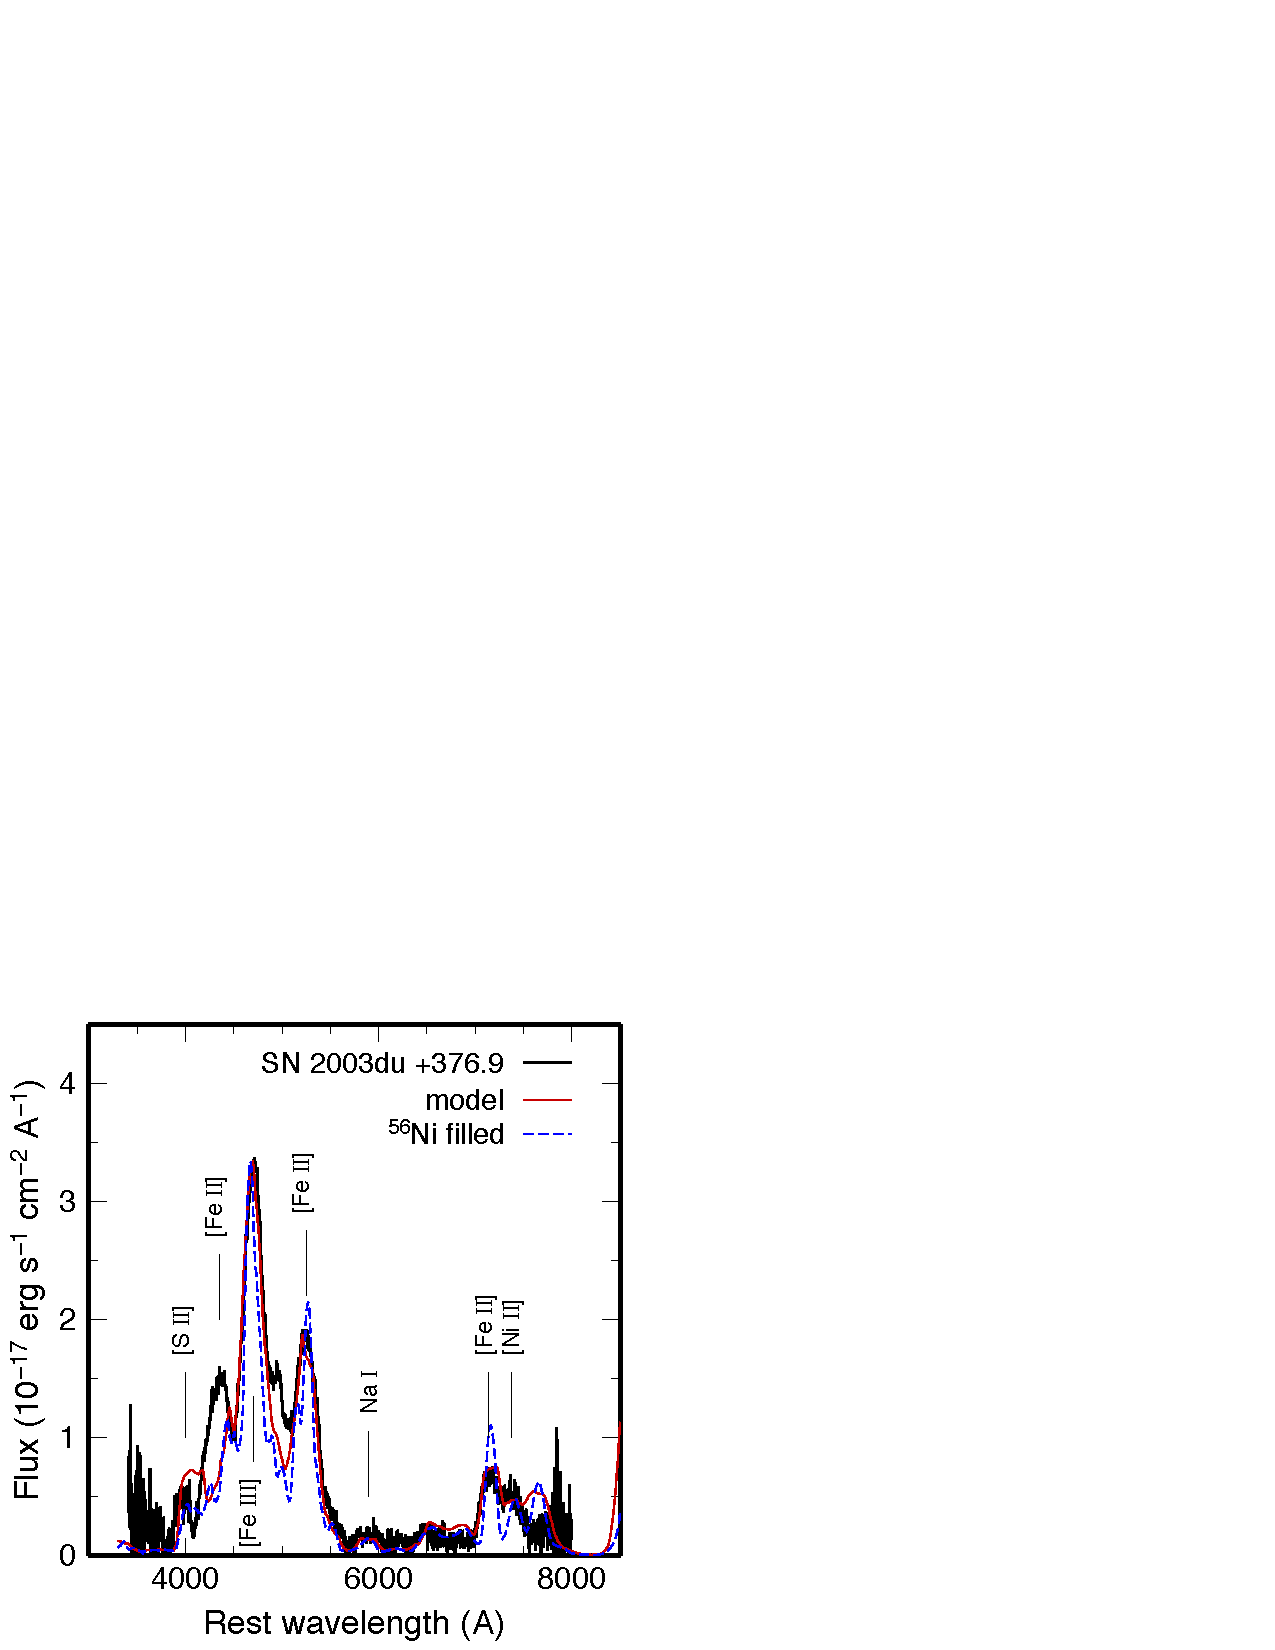
\includegraphics[width=0.45\textwidth]{chapter_intro/plots/sn2003du_nebular.pdf}}
   \caption{Postmaximum evolution of SN 2003du from \cite{2011MNRAS.410.1725T}.}
   \label{fig:sn2003du_t+17}
\end{figure}

\begin{figure}[htbp] %  figure placement: here, top, bottom, or page
   \centering

   \caption{example caption}
   \label{fig:sn2003du_nebular}
\end{figure}



\paragraph{Nebular-Phase}
As the supernova fades, the photosphere disappears. At this stage the spectrum is now characterized by strong emission lines which are produced by the elements from the very core of the explosion (see Figure \ref{fig:sn2003du_nebular}). The velocity has fallen under 5000\,\kms. 




\subsubsection{SNe II Spectra}
\sneii\ show much more variation in their spectra for each object than \sneia\ . In this section we will only give a very general and brief overview over \sneii\ spectra and spectral evolution. 
Compared to \sneia\ the initial spectrum is a relatively undisturbed continuum (see \ref{fig:sn_class_spectra}). The only strong lines visible are those of Hydrogen and Helium which are the elements present in the envelopes of the progenitors. 
As the photosphere recedes into the core heavier elements like Oxygen, Magnesium and Iron become visible. 

The nebular spectra are characterized by $H\alpha$, Oxygen and Calcium emission lines. 

Most knowlege we have about all classes of supernovae we have obtained through optical spectroscopy and photometry. Panchromatic studies of supernovae have been done but are for the moment rare.

\subsection{X-Ray \& Radio observations}

Compared to the traditional optical astronomy X-Ray \& Radio are relatively new fields. The information carried in the very high and low frequency photons is invaluable to understanding various transient events. 

The long \grb-phenomenon has been suggested to be the relativistic jet launched in a \snibc. It is believed that \grb s are visible when this jet poins towards the observer (also known as on-axis). In their late phase \grb 's jet spreads and is thought to emit isotropically in radio. This radio glow should be visible to both on-axis and off-axis observers, but has so far only been observed on-axis . \cite{2006ApJ...638..930S} have tried to find this isotropic radio emission at late times on \snibc\ to see if they are off-axis \grb s. The study however remained inconclusive.

\sneii\ have long been theorized to emit \xray s at shock breakout \citep{1978ApJ...223L.109K,1974ApJ...187..333C}. To observe them is technically very challenging as the supernova needs to be detected very early on. SN2008D was serendipitously discovered by observation with the Swift \xray\ telescope. It was in the process of observing another supernova \sn{2007}{uy} in the same galaxy when  picked up an extremely luminous source \cite{2008Natur.453..469S}. Subsequent ground based follow-up revealed a brightening optical counterpart which turned out to be a \snibc. The \xray-flash was that of the theorized shock breakout of a supernova in a massive star.

\cite{2008Natur.451..802V} have suggested that they found the progenitor of the Type Ia SN 2007on in \xray s. The main caveat speaking against their find was the sizeable distance between the supernova and the \xray-source. Their technique however is promising. Following up \sneia\ in \xray-archives could detect potential \sneia\ progenitors in a pre-explosion \xray\ phase.

Radio and \xray\ observation of both kinds of supernovae are still in its infancy and will provide great help when solving the current mysteries surrounding all types of supernovae.

\subsection{Supernova Cosmology}
Early in the last century astronomers where trying to gauge our place in the universe. \citet{1929PNAS...15..168H} discovered that the Milky Way was not the only galaxy of the universe but found that there were several such galaxies much farther than previously suspected. He used, among other methods, the known intrinsic luminosity ($L_0$) of Cepheid variables and determined using the observed luminosity the distance ($L/L_0 \propto 1/r^2$).  In addition he found that galaxies that were further away had a higher velocity from the Milky Way than close galaxies. He suggested that the universe was in a state of constant expansion. Cepheids distance measurements are only possible for very close-by galaxies and astronomers were feverishly searching for brighter more precise distance probes (also known as standard candles). The discovery that supernovae are distant objects \citep{1934PNAS...20..254B} motivated many astronomers to try to standardize them \cite{1938ApJ....88..285B, 1960ZA.....49..201V, 1968AJ.....73.1021K, 1999ApJ...517..565P}. 

This culminated nearly 70 years later in another paradigm changing discovery. The accelerating expansion universe was discovered, using the same principal but much more advanced technology, by two teams \citep{1998AJ....116.1009R}. 
Since then other techniques have come to the same conclusion \cite[e.g.]{2011MNRAS.tmp..951B}.

\paragraph{\snii\ Cosmology}
\sniip\ have been first suggested as cosmological probes by \citet{1974ApJ...193...27K}. It is important for cosmological distance probes to know the intrinsic luminosity precisely. At the plateau-phase of the supernova, caused by the hydrogen-recombination,  the temperature is well known (T=5000\,K). In addition it is assumed that the supernova is in free expansion, thus a measurement of the velocity and an assumption of the initial radius results in a known radius. Assuming the supernova to be a blackbody during plateau-phase one can then calculate a luminosity using the radius and the temperature. \sniip\ as distance candles, however, are observationally expensive and not as accurate as \snia\ as standard candles (15\% error for \snii  vs 7\% error for \snia\ \citep{2006ApJ...645..841N}).

\paragraph{\snia\ Cosmology}
\sneia\ have been one of the most successful distance probes. It is believed that \sneia\ are the explosion of C-O white dwarfs. The brightness of these objects is powered by the decay of \Ni. The quantity of \Ni\ produced in the explosion can be gauged from the evolution of the light-curve which then in turn can be used to calibrate the intrinsic brightness (see Figure \ref{fig:normalized_lightcurve}).
In the late 1990s new detector technologies (CCDs), computing and new telescopes made it possible to measure the light curves of many \sneia\ accurately. 

The amazing discovery that both \citet{1998AJ....116.1009R} and \citet{1999ApJ...517..565P} made with \sneia\ was that the universe, in stark contrast to the earlier assumption, was expanding at an accelerating rate. 

\begin{figure}[htbp] %  figure placement: here, top, bottom, or page
   \centering
   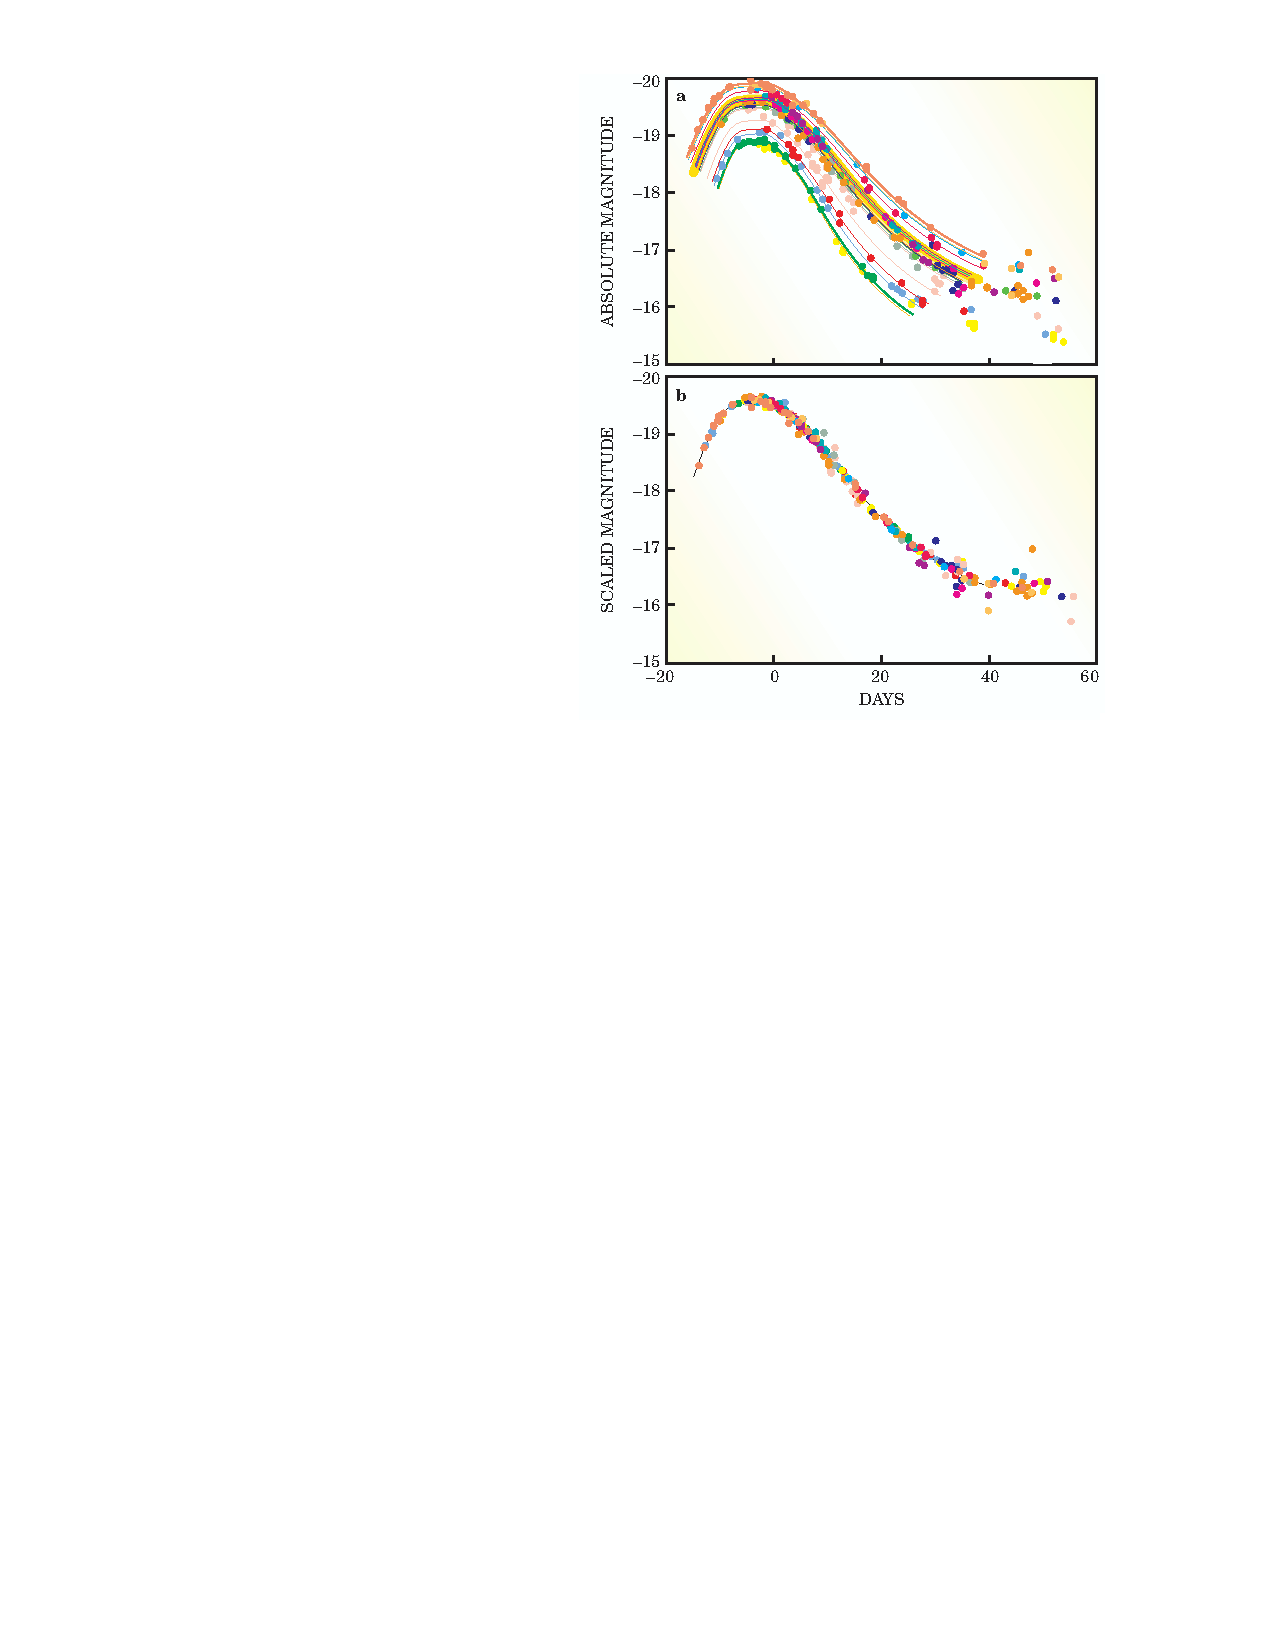
\includegraphics[width=0.7\textwidth]{chapter_intro/plots/lightcurve_scaled_perlmutter2003.pdf} 
   \caption{Replace with some data. any suggestions}
   \label{fig:normalized_lightcurve}
\end{figure}

\section{Post-explosion observations of Supernovae}

In most cases for \sneia, \sneibc\ and \sneii\ the distance to the supernova is too large to make detailed studies of these events post-explosion. 

When supernovae, however, happen in nearby galaxies or in our own. We have the chance of detailed post-explosion follow-up.
SN 1987A, which exploded in the close \lmc\, provided an ideal candidate for follow-up post-explosion which revealed that a previously observed Blue Supergiant was gone post-explosion \cite{1989A&A...219..229W}. This suggests that this star was the cause for the supernova. It was the first time a progenitor was identified with this ``direct detection''-method and since then many more progenitors have been unearthed post-mortem (for a review see 
\cite{2009ARA&A..47...63S}).

Modern X-Ray space telescopes provide data of exquisit detail to study the remnants of supernovae. Hydrodynamic and nonequilibirum ionization simulations of shocks from the supernova ejecta with the \ism\ can be used to measure temperature, elemental abundances and other parameters related to the state of the ejecta \citep{2003ApJ...593..358B, 2004AstL...30..737S, 2005ApJ...624..198B}. This technique of modelling has been used to scrutinize ancient remnants. Kepler and Tycho remnant have been unambiguously identified using \xray-spectroscopy to be remnants of \sneia\ \citep{2006ApJ...645.1373B, 2007ApJ...668L.135R}. This field is still at its infancy and future coupling of three dimensional models with \xray-observations will help reveal the explosions mechanisms for both physical types of supernovae: thermonuclear explosions and core-collapse of massive stars. 

Light-echoes are features that appear when light from a supernova scatters on dust in the \ism. This has been suggested by \citet{1940RvMP...12...66Z}, but only advancements in imaging techniques as well as digital processing made it possible to detect these echoes. \cite{2005Natur.438.1132R} pioneered this technique and found several of these echoes in the \lmc. Follow-up by \cite{2008ApJ...680.1137R} showed that it is possible to obtain a spectrum and identify the type of supernova with it. 
\cite{2008Natur.456..617K} subsequently observed the light-echo of Tycho's supernova (SN 1572) and identified it as a ``normal'' \snia and confirmed the previous \xray-spectroscopy result. Future wide-field surveys will hopefully reveal many more of these light-echoes. Light-echoes can not only be used for classification but also for a three dimensional spectroscopic view of supernovae \citep[demonstrated on the example of Cassiopeia A remnant][]{2011ApJ...732....3R}.

Post-mortem observations of supernovae and their light-echoes provide us with unique insights into these events. For nearby galaxies like the \lmc\ it is possible to scrutinize supernovae using their remnants and echoes which exploded over the last 20,000 years. This in turn can be used to infer rates and \dtd s \citep{2010MNRAS.407.1314M}.
\newpage
\section{Core-Collapse Supernova Theory}

All \snii\ and \snibc\ are believed to be powered by the collapse of the electron-degenerate iron core of massive stars. For the iron core to form there had to be several prior stages of evolution.

\subsection{Evolution of Massive Stars}  To understand the state of the star shortly before supernova evolution it is imperative to follow its evolution. For the topic of core-collapse we will concentrate on the nuclear physics of a single massive star evolution. There has been ample suggestions that some \snii\ and \snibc\ progenitors are binary \citep{1992ApJ...391..246P}, but their evolution is much more complex and is outside the scope of this work.  In this context massive stars are stars bigger than 8 \msun. This is the minimum mass for a star that is believed to explode in a \snii. Like all stars massive stars spend most of their lives on the main-sequence burning hydrogen. This happens via the carbon-nitrogen-oxygen cycle and its various side-channels (e.g $^{12}C(p,\gamma)\rightarrow^{13}N(e^+\nu)\rightarrow^{13}C(p,\gamma)\rightarrow^{14}N(p,\gamma)\rightarrow^{15}O(e^+\nu)\rightarrow^{15}N(p,\alpha)\rightarrow^{12}C$). For a 20 \msun star this phase lasts for 8.13 \myr (see \citet{2002RvMP...74.1015W}).

As the star evolves it begins to ignite Helium which burns via the triple-$\alpha$ process to Carbon ($3\alpha\rightarrow\Carb$) and then to Oxygen ($^{12}C(\alpha,\gamma)\rightarrow\Ox$). Table 1 in \citet{2002RvMP...74.1015W}) lists 1.17 \myr\ for this phase. 

Due to neutrino losses the stellar evolution is qualitatively different after helium burning. A neutrino-mediated Kelvin-Helmholtz contraction of the carbon-oxygen core describes the advanced stages of nuclear burning in massive stars (\citet{2002RvMP...74.1015W}). This contraction is occasionally delayed when the burning of new fuel sources counter-acts the neutrino losses. The star in the end is composited of a series of shells that burn the above fuel and deposit the ashes on the shell below (see Figure \ref{fig:fusion_shells}). There are four distinct burning stages. Their principal fuels are carbon, neon, oxygen, magnesium and silicon.

\begin{figure}[htbp] %  figure placement: here, top, bottom, or page
   \centering
   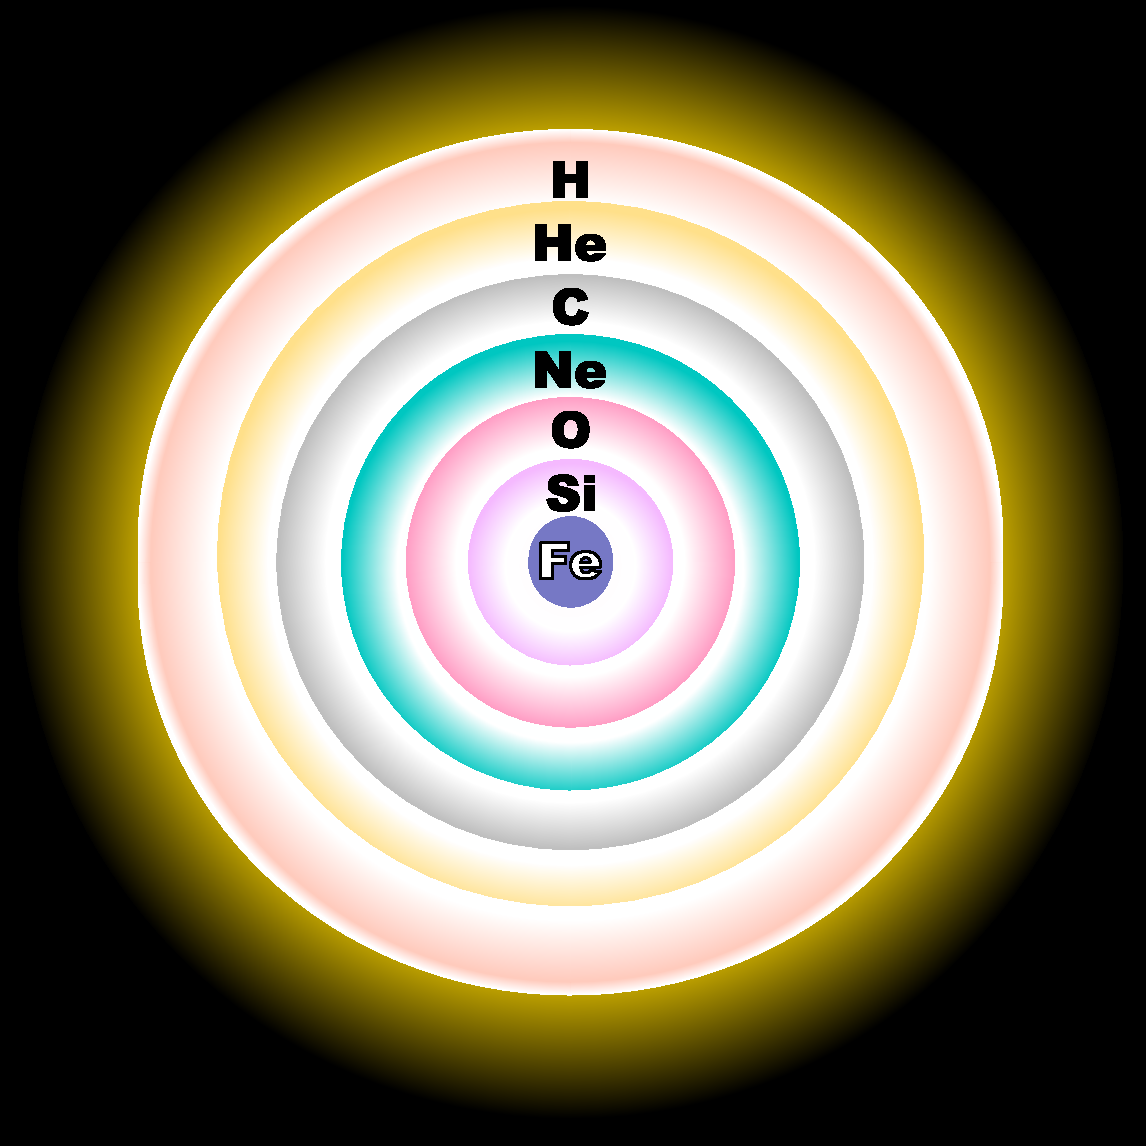
\includegraphics[width=0.5\textwidth]{chapter_intro/plots/fusion_shells.pdf} 
   \caption{Shell Burning of a massive star before \snii. (Source  Wikipedia, Creative Commons License)}
   \label{fig:fusion_shells}
\end{figure}


In the carbon burning stage two $^{12}$C nuclei are fused to an excited state of Magnesium which then decays slowly to $^{23}$Na (see Equation \ref{eqn:c_burning}).
\begin{eqnarray}
^{12}C+^{12}C\rightarrow^{24}Mg&\rightarrow&^{23}Mg+n \nonumber \\
	&\rightarrow&^{20}Ne + \alpha \nonumber \\
	&\rightarrow&^{23}Na +p \nonumber \\
	\label{eqn:c_burning}
\end{eqnarray}

Although oxygen has a lower Coulomb barrier, the next nucleus to burn after Carbon is Neon. This layer is composed of of  $^{16}$O, $^{20}$Ne and $^{24}$Mg and burns Neon with high-energy photons from the tail of the Planck distribution ($\rm ^{20}Ne(\gamma,\alpha)^{16}O$). 

In the next shell there is a composition of mainly $^{16}$O, $^{24}$Mg and $^{28}$Si. The bulk nucleosynthetic reaction is shown in Equation \ref{eqn:c_burning}. 

\begin{eqnarray}
^{16}O+^{16}O\rightarrow^{28}Si&\rightarrow&^{31}S+n \nonumber \\
	&\rightarrow&^{31}P + p \nonumber \\
	&\rightarrow&^{30}P + d \nonumber \\
	&\rightarrow&^{28}Si + \alpha \nonumber \\
	\label{eqn:c_burning}
\end{eqnarray}

The last shell is burning $^{28}$Si to $^{56}$N. The obvious reaction $^{28}\textrm{Si}+^{28}\textrm{Si}\rightarrow^{56}\textrm{Ni}$ does not take place, but is replaced by a very complex network of isotopes to burn to $^{56}\textrm{Ni}$. In simulations this is computationally intensive and numerically unstable (e.g .  \citet{1978ApJ...225.1021W} who carry a 128-isotope network). 
Following silicon burning the composition consists of mainly iron-group nuclei. 
At the end of silicon burning we are reaching nuclear statistical equilibrium. 

\subsection{Core collapse} Before the collapse,  the core consists of iron peak elements. Neutrino losses during carbon and oxygen burning decreased the central entropy sufficiently so that the core becomes electron degenerate. Such a degenerate core, which is higher than the Chandrasekhar mass (adjusted for Y$_e$, entropy, boundary pressure and other parameters) will collapse. 

There are two main instabilities that facilitate the collapse. As the density rises the Fermi-Energy becomes high enough for electrons to capture onto iron-group nuclei. This capture process removes electrons that were providing degeneracy pressure and reduces the structural adiabatic index. 

The second instability is the rise to temperatures where the nuclear statistical equilibrium favours free $\alpha$-particles. The collapse eventually leads to nuclear densities, the hard-core potential acts as a stiff spring during the compressive phase. It stores up energy and eventually releases this energy resulting in a "core bounce".  
\citet{1985PhRvL..55..126B,1987PhRvL..59..736B} believed the core bounce to provide the energy for the ensuing supernova explosion. More recent simulations however show that the bounce shock is not sufficient for a \snii\ explosion. The bounce shock looses energy by photo disintegrating the nuclei it encounters (loosing roughly $10^{51}$\,\erg\ per 0.1\,\msun).

The energy for a successful explosion is now thought to come from neutrino energy deposition. This reinvigorates the shock and leads eventually to an explosion which ejects the envelope of the massive star. \cite{2007ApJ...655..416B} suggest that instead of neutrinos, acoustic waves might heat up the ejecta and cause the explosion. In any case a newly born neutron star is left behind.

The precise explosion mechanism is unknown. Using progenitor models with different parameters like rotation and mass lead to different outcomes. \citet{2002RvMP...74.1015W} provide a very comprehensive review of the theory of evolution and core collapse. In particular they go into more detail describing the scenarios after core-bounce.

\subsection{Pair instability}
One alternate explosion scenario is the pair-instability supernova. This scenario is believed to only happen in stars with a helium core of more than 40\,\msun. After core helium burning the star starts to contract at an accelerated rate. The energy release during this process is used to produce electron-positron pairs rather than raising the temperature. If significant densities are reached, oxygen fusion eventually halts the implosion and the collapse bounces to an explosion. For very high stellar masses it is believed that oxygen fusion does not provide enough energy to halt the contraction and the star collapses to a black hole.


\subsection{Type II Supernovae}
The observables of these stellar cataclysm are the light curve, spectra and for one case even the neutrino wind. The supernovae goes through three distinct phases which can be observed. 

The shock-breakout is the first visible signal from the supernova.  \cite{1992ApJ...393..742E} calculated a duration for the  shock breakout of SN1987A to 180\,s three minutes, its  luminosity of $5\times10^{44}$\erg\,s$^{-1}$. 
Thus far it has been observed only once in 2008D \citep{2008Natur.453..469S}. They report a duration of 400\,s with a luminosity of $6.1\times10^{43}$\erg\,s$^{-1}$.

The plateau seen in many \snii\ (see Figure \ref{fig:snii_lc}) is produced by the recombination of hydrogen when hydrogen-rich zones cool to less than 5500\,K. The radiation comes effectively from a blackbody, whose luminosity is determined  by the radius of the photosphere.
Supernovae of Type IIL do not show this behaviour and are thus thought to have no or a very small hydrogen envelope.


After the recombination of hydrogen the light-curve drops off linearly and we see radioactivity providing the main energy source. \Ni\ decays to \Co\ with a half-life of 6.1\,d and then further to \Fe\ with a half-life of 77\,d. Most of the energy of the \Ni\ decay is used to accelerate the expansion of the core. The tail of the light-curve after the plateau is mainly powered by the decay of \Co. Some light be also produced by shock interaction with the \csm.





\subsection{Type Ib/c supernovae}
If the star lost all of its hydrogen envelope prior to core-collapse there is no plateau visible in the light-curve. Instead the light-curve is powered by radio-active decay after shock breakout. In addition, the hydrogen lines are not visible in the spectrum. This leads to the supernova being classified as Type Ib. If both hydrogen and helium envelopes are lost then the supernova is classified as Type Ic. 
This loss of envelope is presumed to be caused by stellar winds or binary interactions \citep{1992ApJ...391..246P}. 


\section{Thermonuclear Supernova Theory}
In this section we will discuss the theory of \sneia\ which are thought to be thermonuclear explosions of degenerate Carbon/Oxygen matter. The different progenitor scenarios leading to an explosion of a massive white dwarfs are discussed in Section \ref{sec:snia_progenitor}.

\subsection{White Dwarfs}
\label{sec:white_dwarfs}
Carbon/Oxygen white dwarfs are thought to be the progenitor stars of \sneia. White dwarfs are among the few stellar objects that do not hold hydrogen. This would explain the lack of hydrogen in \snia-spectra. It is general believed in the community that these objects accrete matter (for the possible scenarios see section \ref{sec:snia_progenitor}) until they get close to the Chandrasekhar-mass \citep[henceforth \mchan;][]{1931ApJ....74...81C}. It is a delicate balance between the ignition point that results in the thermonuclear run-away and the Chandrasekhar threshold which leads to a collapse of the star to a neutron star.
 
There are three main classes of white dwarfs: Helium, Carbon/Oxygen (henceforth \cowd) and Oxygen/Neon (henceforth \onemgwd) white dwarfs. Helium white dwarfs would start burning their Helium to Carbon and Oxygen well before it gets near the Chandrasekhar mass. In addition, these objects can also be ruled out as progenitors for \sneia\ as copious amounts of \ige\ produced in \sneia\, which are not consistent with the burning of a Helium white dwarf. 

The ultimate fate of an \onemgwd\ is thought to be the collapse into a neutron star. Once the \onemgwd\ is heavy enough electron capture begins in the core ($\Ne(e^-,\nu)\F[20](e^-,\nu)\Ox[20]$). Heating by the resulting $\gamma$-rays starts explosive Oxygen burning. However, the electron-capture is much faster than the Oxygen burning and promotes the collapse to a neutron star \citep{1991ApJ...367L..19N, 2005A&A...435..231G}. 

The favoured progenitor for a \snia\  are \cowd s. Most of these objects are born, however, with a mass around 0.6 \msun\ \citep{2007MNRAS.375.1315K}. It is thought that they accrete mass until they are getting close to the Chandrasekhar mass and then explode as a \snia.

\subsection{Pre-supernova evolution}
The white dwarf gradually accretes more and more material. Close to \mchan mild carbon burning ensues
\begin{align}
\nonumber
\Carb(\Carb,p) &\rightarrow \Na \\  \nonumber
\Carb(\Carb,\alpha) &\rightarrow \Ne \\ 
\Carb(\Carb,n) &\rightarrow \Mg[23]
\end{align},
but is mediated by photon and neutrino loses \citep{2005NuPhA.758..463L, 2007nps..book.....I}. As the cooling processes become less effective convection starts in the core. The energy output in the core increases. At this stage the thermal structure is largely controlled by Urca pairs. These reaction pairs consist of alternating electron captures and $\beta^-$\,-decays involving the same pair of parent and daughter nuclei. Two prominent examples which are important in pre-supernova evolution are \Ne[21]/\F[21]:
\begin{align}
\nonumber
\Ne[21](e^-, \nu) &\rightarrow \F[21] \\
\F[21](\beta^- \nu) &\rightarrow \Ne[21]
\end{align}
These processes can lead to either cooling or heating. \cite{2005NuPhA.758..463L} have modelled this process in a convective core. 

Ultimately, the pre-supernova evolution is hard to model theoretically as it is likely to be nonlocal, time-dependent, three dimensional and stretches over hundreds of years. The exact conditions at the time of explosion are therefore unknown. All explosion models have to assume simple initial conditions. 

\paragraph{Ignition}
The \urca processes will dominate core evolution for the last thousand years until explosion. As the temperature rises to $T\approx7 \times 10^8$\,K \citep{2000ARA&A..38..191H} the convection time ($\tau_c$) increases and becomes comparable to the burning time ($\tau_b$). Consequently the convective plumes burn as they circulate. Once the temperature reaches $T\approx 10^9$\,K $\tau_b$ becomes very small compared to $\tau_c$ and Carbon and Oxygen essentially burn in place. 
This is the moment of ignition. As the convective plumes burn while they rise it is likely that the initial flame seed does not start in the center of the core. \cite{2005A&A...431..635R} have used multiple flame seeds in their three dimensional full star models.

\paragraph{Thermonuclear Explosion}
From this point, initially there were two main options. The first option was the complete detonation (supersonic flame front) of the \cowd\ \citep{1969Ap&SS...5..180A}. It was quickly, discovered, however that this method burns to \nse\ and thus produces no \ime. These \ime\ are observed in \snia.

For a long time it was then suspected that the star instead of detonating would deflagrate (subsonic flame wave, mediated by thermal conduction). The fuel in front of the deflagration gets rarified by the energy from the flame. Hot light burning bubbles rise into the cold dense fuel and create Rayleigh-Taylor instabilities (see Figure \ref{fig:snia_ddt_roepke2007} at t=0.72\,s). 
Once the deflagration wave has run through the star, the resulting production of \Ni[56] is not enough to explain the light curve of normal \snia. The deflagration produces roughly 0.3\,\msun of \Ni[56], to power the light curve of normal \sneia\ one needs 0.6\,\msun \citep{2007Sci...315..825M}.

The currently favoured scenario is the one of delayed detonation. The star initially burns like in the deflagration scenario, then inhomogeneities in the deflagration front produce hotspots. In these hotspots the temperature gradients are so high that detonation waves form. The ensuing detonation front can only burn the cold unburnt-fuel and does not penetrate the ashes of the deflagration. Figure \ref{fig:snia_ddt_roepke2007} shows clearly how the detonation wave wraps around the cold ashes over the course of the detonation.


\begin{figure}[htbp] %  figure placement: here, top, bottom, or page
   \centering
   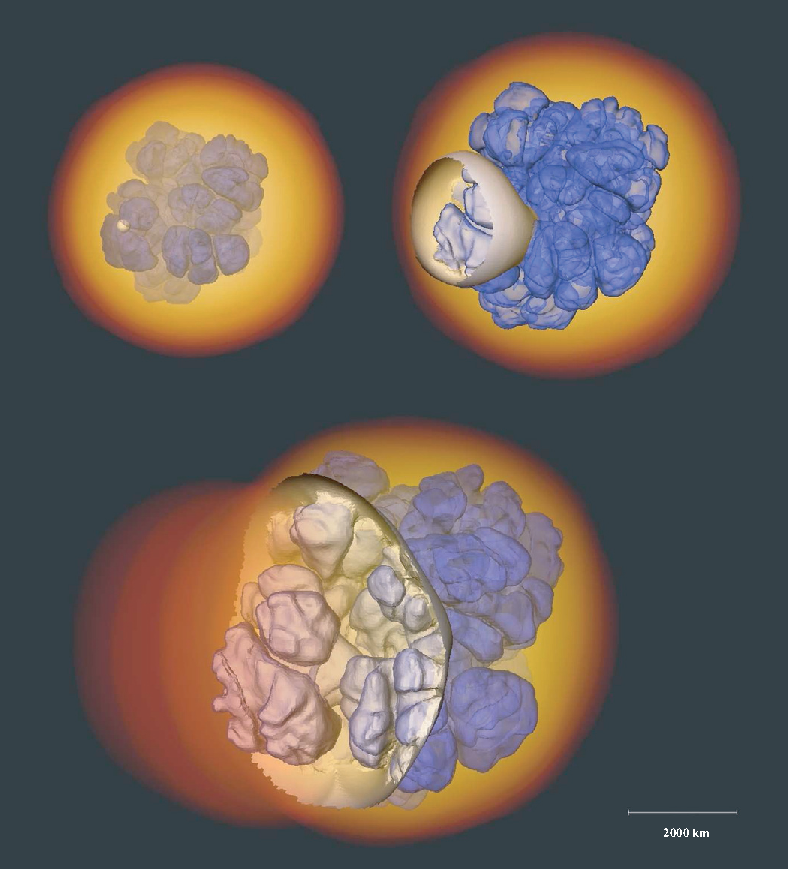
\includegraphics[width=0.7\textwidth]{chapter_intro/plots/ddt_roepke08.pdf}
   \caption{ Delayed detonation simulation from \citet{2008NJPh...10l5009R}. The upper panels show the deflagrated interior (marked in blue) and the detonation ignition point (small white sphere). The detonation wave wraps around the deflagration ash and consumes the cold fuel. (Image reproduced with kind permission of Fritz R\"{o}pke)}
   \label{fig:snia_ddt_roepke2007}
\end{figure}

An open question is if and how these transitions from deflagration to detonation occur in \sneia. This scenario reproduces the light curves and spectra reasonably well \citep{2009Natur.460..869K}. 


\paragraph{sub-Chandrasekhar-mass detonations}
\label{sec:subchandra}
\citet{1992ApJ...386L..13S} and \citet{2010ApJ...714L..52S} have explored the detonation of \cowd s at sub-Chandrasekhar masses.  \citet{2010ApJ...714L..52S} show that the detonation of a sub-Chandrasekhar-mass \cowd\ reproduce observed light-curves and early-time spectra of \sneia\ fairly well.

The main issue in this scenario is the ignition. \cite{2010A&A...514A..53F} have suggested an explosion mechanism in which a surface detonation of a Helium shell drives a shock-wave into the core. In the core this shockwave triggers an ignition by compression.  As an initial model they use a \cowd\ accreting from a helium rich companion building a thin helium shell around its CO interior \citep[described in][]{2007ApJ...662L..95B}. This helium shell is ignited and sends out a shockwave. As the helium flame spreads on the shell around the star it sends a shockwave into the core. Once 
the shockwaves converge off-center they create a the right environment for the ignition of a detonation wave (see Figure \ref{fig:subch_fink2010}.) 

This scenario reproduces the intrinisic luminosity variability in the class of \snia\ as each exploding white dwarf can have a different mass. 

\begin{figure}[htbp] %  figure placement: here, top, bottom, or page
   \centering
   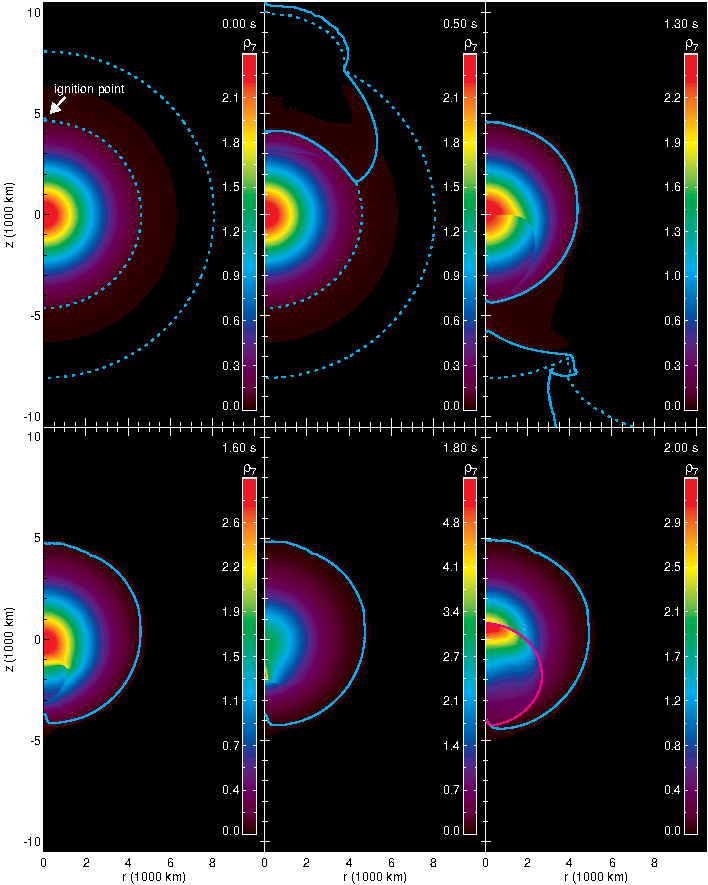
\includegraphics[width=0.7\textwidth]{chapter_intro/plots/fink2010.pdf} 
   \caption{The ignition point of the helium shell is marked in the upper left image. We can follow the helium shell sending shock waves into the core of the white dwarf. They converge in the lower left image at the opposite site of the Carbon/Oxygen core \citep[data from][figure kindly provided by Michael Fink]{2010A&A...514A..53F}. }
   \label{fig:subch_fink2010}
\end{figure}

\paragraph{\WD-\WD\ mergers}
\cowd\ mergers for a long time were thought to lead to a gravitational collapse \citep[same mechanism as the \onemgwd][]{1985A&A...150L..21S}. \citet{2010Natur.463...61P} has, however, successfully simulated the explosion of two merging \cowd s. The initial model was two equal mass 0.8\,\msun\ \cowd s. The merging process created a hotspot from which a detonation wave eminates. 
The resulting light-curves and spectra are faint and are similar to the class of sub-luminous \snia. 


\section{Progenitors of Type Ia Supernovae}
\label{sec:snia_progenitor}

\citet{1973ApJ...186.1007W} first introduced the modern binary evolution paradigm for \snia-progenitors. In their model a \cowd\ accretes matter from a red giant. A degenerate \cowd\ accreting from a non-degenerate companion is now known as the single degenerate scenario. 

\citet{1984ApJ...277..355W, 1984ApJS...54..335I} were the first to suggest that the merging of two \cowd s could also produce \sneia. This scenario is now commonly referred to as the double degenerate scenario.



\subsection{Single Degenerate Scenario}
The single degenerate scenario assumes a binary system with one evolved white dwarf and one non-degenerate companion. In most cases this non-degenerate companion is thought to be main-sequence to red giant. There are scenario that involve "exotic" companions such as helium stars. The companion (or donor) star is believed to have filled its Roche-Lobe and lose mass via Roche-Lobe-Overflow (henceforth \rlof).

\subsubsection{Accretion}
The main problem of the \sd-scenario is the accretion process.  As most white dwarfs are born with masses around 0.6\,\msun they need to accrete mass to reach the critical 1.38\,\msun. The process needs to be efficient as well as burn most accreted hydrogen to explain its lack in the spectrum.
 If the mass-accretion rate is too low it causes nova explosions which are thought to eject more mass than they had accreted prior \citep{Nomoto:1982p451}. There are however systems (e.g. RS Oph, U Sco) that have white dwarf masses close to 1.4\,\msun\ which have recurrent nova outbursts. It is very likely that these systems weren't born with a white dwarf that massive, but that these white dwarfs accreted the material. This suggest that despite nova outbursts efficient accretion is possible. 
 
 Too high accretion rates would engulf the binary in an extended red giant envelope which would promote a merger of the two compact objects. Debris of such an envelope is not seen in \snia-explosions. If To avoid this merger the system would have to loose the excess mass in a wind. This again results in a low accretion rate. There is only a very narrow range of accretion rates that allows the white dwarf to accrete hydrogen, stably burn it and efficiently accrete to \mchan. \cite{2004A&A...419..623Y} have suggest that rotation of the accreting white dwarfs might increase this very narrow parameter range.
 
A class of binaries called Supersoft X-Ray sources (\sss) might accrete hydrogen at a sufficiently high rate. At this rate Hydrogen and Helium burn hydrostatically, if retained, make these objects very strong contenders for \snia\ progenitors \citep[][and references therein]{2006astro.ph..6364D}. 
 
Another subclass of \sd-progenitors are AM CVn stars. These type of cataclysmic variable accretes from a helium star \cite{1992A&A...262...97V}. This scenario would very conveniently explain the lack of hydrogen in \snia-explosions. \citet[][]{2010A&A...514A..53F} have found a way that such systems can explode in a \snia (see Section \ref{sec:snia_theory}).


\subsubsection{Donor Stars}
The \sd-scenario requires a secondary companion (also known as donor) star. If this companion survives the explosion it would be a calling card for the \sd-scenario. 

\citet{2000ApJS..128..615M} have simulated the impact of \snia-ejecta on main-sequence, sub-giant and red-giant companion. In the case of the main-sequence companion the supernova ejecta heats a small fraction (1-2\%) of the envelope which is lost post-explosion. \citet{2008A&A...489..943P} have repeated the simulations for the main-sequence companion and find similar results, but suggest that less mass is lost. Post-explosion the star could be very luminous (500 -- 5000 \lsun). It is expected to cool down between 1400 -- 11000 yrs and follow the main-sequence track. 

For the sub-giant companion the simulations show very similar results to the main-sequence companion. In summary, the subgiant looses only a small fraction of the envelope (10 -- 15\%) and similar to the main-sequence star will be very luminous shortly after the explosion. After thermal equilibrium is established the companion will return to a post-main-sequence track. 

The case of the red-giant, however, is very different. \citet{2000ApJS..128..615M} suggest that it will loose most of its loosely bound envelope. Post-explosion the remaining core rises contracts and the temperature rises to more than $3 \times 10^4$\,K. The object may appear as an under luminous main-sequence O or B star. 


\cite{2009A&A...493.1081J} have suggested low-mass single white dwarfs to be the remaining cores of red-giant donor stars. This would result in a convenient explanation for the existence of these objects. 

One feature of surviving companions may be an unusually large rotational velocity post-explosion \citep[][chapter \ref{ch:sn1572_starg} of this work]{2009ApJ...701.1665K}. Due to tidal coupling during the \rlof-phase one calculate the expected rotational velocity from the escape velocity of the donor (see Figure \ref{fig:theorot}). Late-type stars usually don't display such high rotational velocities. Thus this feature is a very useful discriminant when looking for donor stars. 

Most simulations suggest that the donor-star would survive the explosion one way or another. There have been several attempts to find these objects in ancient supernova remnants. \citet{1980ApJ...241.1039S} found a OB subdwarf star located 2.5 \arcmin from the center of the remnant of SN1006 and suggested this as the donor star. Subsequent analysis by \cite{1997ApJ...477L..53W, 1983ApJ...269L...5W} have however revealed however strong red and blue shifted iron lines. The velocities of these lines are on order of 5000\,\kms which is the same as the velocity of the freely expanding remnant of \sn{1006}. This suggests the star to be located behind the remnant.
 
The search of donor stars in ancient remnants is one of the main parts of this thesis and we direct the reader to chapter \ref{chap:sn1572_starg} and chapter \ref{chap:sn1572_hires}.



\subsection{Double Degenerate Scenario}
\citet{1984ApJ...277..355W} and \citet{1984ApJS...54..335I} were the first to suggest merging white dwarfs as progenitors for \snia. There are several advantages to the \dd-scenario. For example, it naturally explains the lack of hydrogen in \snia-spectra. The accretion problem encountered in the \sd-scenario are also eleviated with \dd-scenario, as long as the sum of masses of both \cowd's is above \mchan. 

The problem, however, is that most \snia\ are relatively homogeneous. It is hard to reconcile this fact with the merger of two white dwarfs with different initial masses, composition, angular momenta and different impact parameters. Another caveat, however, is that the accretion of the disrupted lighter white dwarf onto the more massive white dwarf might lead to the transformation into a \onemgwd (see section \ref{sec:white_dwarfs})

\cite{2010Natur.463...61P} have simulated the merger of two equal-mass white dwarfs (0.8\,\msun) and conclude that the outcomes of these mergers might be subluminous \sneia.

In summary, mergers of white dwarfs might be able t explain some of \snia. It is however still debated if these events are responsible for the ``normal'' \sneia. 

\subsection{Constrains for different progenitor scenarios}

Radio observations in the case of \sneia\ can for example reveal the shock interaction of the ejecta with the \csm. The single degenerate scenario predicts more \csm than the double degenerate scenario. \citep{2011arXiv1105.6188H} have stacked radio observations of \sneia\ in the visibility plane. They can not detect any source. This could hint that the double degenerate scenario is the more common, but many caveats remain.

On the other hand however \cite{2007Sci...317..924P} have found variable Sodium features using high-resolution spectra of \sneia. These hint at the evolution of the Sodium ionization state in the \csm caused by the variable \snia\ radiation field. A wind from the donor star would provide material with the right geometric distribution to reproduce these features. Recently \cite{2011A&A...530A..63P} have seen similar features in the recurrent nova RS Ophiuchi. This could hint that recurrent novae with red giant donor stars might be responsible for some \sneia. 


\cite{2010ApJ...708.1025K} predict excess in UV flux in the \snia light curve at early times. This effect depends on orientation of the system to the line of sight and the state of the donor. The effect would be biggest for a giant donor. \cite{2010ApJ...722.1691H} do not see this excess in the SDSS supernova set. This suggests that the red giant channel is not common for \sneia\ and might suggest that \dd-scenario is predominent. There remain, however, many caveats. The orbits of the \sd-system might be closer than expected (suggesting that the existing light-curve data is not early enough) or the effect overestimated.

It remains a mystery that \sneia\ do not show lines of Hydrogen which might be expected from the wind or stripped envelope in the \sd-model. \citet{2007ApJ...670.1275L} have searched in the nebular spectra of two \sneia\ for hydrogen and place an upper limit of 0.1\,\msun\ for both these explosions. One might take this as a further hint against the \sd-scenario. On the other hand \citet{2011ApJ...730L..34J} suggest that a red giant donor could significantly shrink during the \rlof. This would place the the stripped hydrogen below the current detection limit. 

\cite{2010ApJ...719..474D} have not found enough \sss, which are suggested \snia-progenitors for the \sd-scenario. In addition, \cite{2010Natur.463..924G} have not found enough accumulated X-ray flux from elliptical galaxies if all \snia-progenitors were \sss\ (assuming the X-Ray flux calculated for these objects is correct). The main caveats are that the \snia-progenitors might only be in the \sss-phase for a moderate amount of time. In addition, these objects could be engulfed in a envelope, which would reprocess the produced \xray s to optical or infrared wavelengths.

Finding a donor star of the \sd-scenario in a \snr\ post-explosion, would resolve the question for the progenitor system at least in the searched remnant. The main work of this thesis investigates this technique and we will refer the reader to Chapters \ref{chap:sn1572_starg,chap:sn1572_hires, chap:sn1006}. 

Population synthesis together with observations of \dtd s are an important step in exploring the different progenitor scenarios. \citet{2008ApJ...683L.127H, Han:2004p444}  and suggest when compared to observations that the \sd-scenario is not far from explaining the observed \dtd\ (for references on \dtd\ see section \ref{sec:sn_rates}). 
\citet{2009ApJ...699.2026R, 2010A&A...515A..89M}, however, have explored the \snia-rate using several progenitor scenarios (\sd, \dd\ and \amcvn). Both suggest that the \sd-scenario on its own can not explain the observed \sneia-rate. The \dd-rate seems to be much closer to the observed frequency. Possibly a mix of all channels is required to explain the observed rate. 

In summary, the question of the progenitors is currently one of the most highly debated in \sneia\ research. There exist multiple arguments for both the \sd-scenario and \dd-scenario. In addition, new scenarios like the core-degenerate system in which a white dwarf merges with the hot core of a massive \agb\ star \cite{2011arXiv1106.2027I} are emerging. \cite{2011arXiv1102.4342D} and \citet{2011ApJ...730L..34J} suggest that the accreting white dwarf would be spun-up during accretion. The ignition of these highly spinning white dwarfs would be delayed and the companion might have time to evolve. This might possibly forfeit some of the arguments brought against the \sd-scenario. 
\cite{2010ApJ...722L.157V} on the other hand suggests the merger of two equal mass white dwarfs with a total mass less than \mchan. There remain still many caveats, but coupled with the work on sub-Chandrasekhar mass detonations by \citet{2010ApJ...714L..52S}, this might provide an interesting scenario. The main advantage is the predicted rate of these low-mass white dwarf mergers might be high enough to reproduce the observations.
More and novel observations of \sneia\ and \snr\ will hopefully help constrain the progenitor scenario. In the community some astronomers are now suggesting a multi-channel approach to explain \sneia\ phenomenon.
 

\newpage
\section{Thesis motivation}
One of the most pivotal moments in astronomy in recent years was the discovery of the acclerating expanding universe by \citet{1998AJ....116.1009R} and \citet{1999ApJ...517..565P}. This discovery catapulted \sneia\ into the limelight of the astronomical community. There has been many advances in recent years in the understanding of these cataclysmic events (explosion models, rates, etc.). One critical piece of the puzzle, however, has so far eluded discovery: The progenitors of \sneia. This work's main aim is to find evidence for one \snia-progenitor scenario. The \sd-scenario proposes a white dwarf accreting from a non-degenerate donor star. To the best of our knowledge this donor star is thought to survive the explosion and would be visible thereafter. We have tried to find this companion in two of three easily accessible ancient supernova remnants (SN1572 and SN1006). 
In chapter \ref{ch:sn1572_starg} we have obtained spectra of \starg\ which had been suggested as the donor star of SN1572 \citep{2004Natur.431.1069R}. Although we confirmed some of the suggested parameters we could not reproduce the unusually high radial velocity which led to the claim. 

We revisited SN1572 in chapter \ref{ch:sn1572_hires} with new observations of \starg\ and five other stars in the neighbourhood of SN1572. This resulted in \starg\ to be not a very viable donor star (it is hard to completely rule stars out). We discovered a curious A-Star located serendipitously right in the center of SN1572. Despite its bizarre parameters we could not reconcile this star (\starb) with any feasible progenitor model. We, however, found a scenario which explains \starb's features but does not involve it in SN1572. 

SN1006 provides a perfect opportunity to search for progenitor stars. It is the closest known remnant of a \snia\ (2\,kpc). We have obtained 80 spectra of stars close to the center of the remnant and present them in chapter \ref{ch:sn1006}. Again we did not find any obvious donor stars. 

We have obtained spectra of stars around SN1604 but these are not presented in this work.

Progenitor hunts provide us with information of the scenarios pre-explosion. Spectra on the other hand help to unravel the happenings during and post-explosion. \cite{2008MNRAS.386.1897M} have developed a code that can produce synthetic \snia-spectra from fundamental input parameters. Fitting an observed \snia\ is for the moment a manual task. This requires many days, if not weeks, of tweaking. The deluge of spectroscopically well-sampled \sneia\ from surveys is already hitting us. Manual analysis of all these spectra is impossible. The information about the explosion hidden in the spectra is, however, crucial to our understanding of these events. In chapter \ref{chap:dalek} we present our work towards automating this fitting process. We have tried a variety of algorithms to explore the vast and extremely complex search space. Working together with members of the computer science community we are exploring the use of genetic algorithms to solve this problem. 
This work is not finished yet, but we present preliminary methods in \snia-fitting in chapter \ref{chap:dalek}. Once finished we can apply this method not only in fitting \snia, but fitting other supernovae and in other areas of astronomy. 

In summary, this work explores two areas of supernova physics. The hunt for progenitors has not yielded obvious candidates, but may suggest a rethinking of the "normal" \sd-scenario. The automation of the supernova fitting is in its infancy stage. We have however shown that it is possible to explore the space in an automated fashion. This will hopefully yield abundances and energies for many thousand supernovae. 
The close collaboration with computer science community has shown how important cross-disciplinary research is in this era of science. 



% !TEX root =../thesis.tex
\chapter{SN1572}
\label{chap:SN1572}

\section{Introduction}
Type Ia supernovae (SNe Ia) are of broad interest. They serve as
physically interesting end points of stellar evolution, are major
contributors to galactic chemical evolution, and serve as one of
astronomy's most powerful cosmological tools.

It is therefore unfortunate that the identity of the progenitors
of SNe Ia is still uncertain. For example, without knowing the progenitors,
the time scales of SNe Ia enriching the interstellar medium with iron
remains highly uncertain. But it is the crippling impact on the
cosmological application of these objects which is especially
profound; it is impossible to predict the consequences of any
cosmological evolution of these objects or even gauge the likelihood of
such evolution occurring.

There is broad agreement that the stars which explode as SNe Ia are
white dwarfs which have accreted material in a binary system until
they are near the Chandrasekhar mass, then start to ignite carbon
explosively, which leads to a thermonuclear detonation/deflagration of the
star. It is the identity of the binary companion that is currently
completely undetermined. Suggestions fall into two general categories
\citep{1997thsu.conf..111I}:
\begin{itemize}
\item Single degenerate systems in which a white dwarf accretes mass
from a non-degenerate companion, where the companion could be a
main-sequence star, a subgiant, a red giant, or possibly even a
subdwarf.
\item Double degenerate systems where two CO white dwarfs merge,
resulting in a single object with a mass above the Chandrasekhar limit.
\end{itemize}

The detection of circumstellar material around SN~2006X
\citep{2007Sci...317..924P} has provided support for the single
degenerate model in this case, although the lack of substantial 
hydrogen in several other SNe Ia \citep{2007ApJ...670.1275L} 
poses more of a challenge to this scenario.

These models also make different predictions for the nature of the system
following the explosion. In the double degenerate case, no stellar
object remains, but for a single white dwarf, the binary
companion remains largely intact.

In the single degenerate case, the expected effect of the SN on the
donor star has been investigated by \citet*{2000ApJS..128..615M}, who
have calculated the impact of a SN Ia explosion on a variety of binary
companions. \citet*{2001ApJ...550L..53C} have explored many of the
observational consequences of the possible scenarios, and
Podsiadlowski (2003) has presented models that follow both the
pre-supernova accretion phase and the post-explosion non-equilibrium
evolution of the companion star that has been strongly perturbed by
the impact of the supernova shell.  To summarize these results,
main-sequence and subgiant companions lose 10\,--\,20 \% of their
envelopes and have a resulting space velocity of 180\,--\,320\,\kms . Red-giant companions lose most of its hydrogen envelope, leaving a
helium core with a small amount of hydrogen-rich envelope material behind,
and acquire a space velocity of about 10\,--\,100\,\kms.
\citet{2008A&A...489..943P} have used a binary stellar evolution code on a main-sequence star and exposed the evolved star to a SN Ia. Their simulations show that even less material is stripped due to the compact nature of a star that evolved in a binary. We will use their results where applicable. 

\citet[henceforth \rl]{2004Natur.431.1069R} have identified what might
be the donor star to Tycho's SN, a SN Ia which exploded in the Milky
Way in 1572. These authors presented evidence that this star, \starg\
by their naming convention, is at a distance consistent with the Tycho
supernova remnant (henceforth SNR), has a significant peculiar radial
velocity and proper motion, roughly solar abundance, and a surface
gravity lower than a main-sequence star. However, \starg\ is located at a significant distance from the
inferred center of the remnant, and any process that has displaced the
star must preserve the remnant's nearly perfectly circular projected shape. During the final stages of refereeing of this paper we were made aware of the article by \citet[henceforth \gh]{2009ApJ...691....1H}, who used Keck HIRES data to better constrain \starg's stellar parameters, and in addition, found an enhancement in Nickel abundance, relative to normal metal rich stars.

\citet{2007PASJ...59..811I} have looked for Fe absorption lines from
the remnant, using nearby stars as continuum sources, with the hope to
better constrain the distance of these stars to the SNR. With their technique, stars in the
remnant's center should show strong blue-shifted Fe absorption lines,
formed by material in the expanding shell of Fe-rich material from the
SN, moving towards the observer.  Stars in the foreground would show
no Fe absorption, and background stars both red- and blue-shifted
absorption. Their study shows that \starg\ does not contain any
significant blue-shifted Fe absorption lines, suggesting that \starg\
is in the remnant's foreground. However, these observations and their
analysis, while suggestive, cannot be considered a conclusive rebuttal
of \starg's association with the remnant; this technique requires a significant column depth of Fe which is not guaranteed. A lack of Fe column depth may be indicated by the fact that no stars were found in the
vicinity of the remnant that showed both blue- and red-shifted absorption lines.

To further examine the \rl\ suggested association of \starg\ with the
SN Ia progenitor, we have obtained a high-resolution spectrum of the
star using Subaru and its High Dispersion Spectrograph
\citep{1998SPIE.3355..354N}.

We summarize, in section 2, the observational
circumstances of the Tycho remnant and any donor star, and argue in
section 3 that rapid rotation is an important, previously unrealised
signature in a SN Ia donor star. In section 4 we describe our
Subaru observations. Section 5 covers the analysis of data and the results of this analysis. Section 6 compares the relative merit for \starg\ being the donor star to the
Tycho SN or being an unrelated background star, and in section 7 we summarize our findings and motivate future observations.

\section{Observational Characteristics of the Tycho Remnant and Star-G}

\rl\ have done a thorough job summarizing the relevant details of the
Tycho remnant. The remnant shows the characteristics expected of a SN
Ia based on its light curve (measured by Tycho Brahe himself),
chemical abundances, and current X-ray and radio emission
\citep{2004ApJ...612..357R}. In figure \ref{fig:overview} we have overlaid radio contours\footnote{The National Radio Astronomy Observatory is a facility of the National Science Foundation operated under cooperative agreement by Associated Universities, Inc.}  on an optical image and have marked the position of the stars mentioned in this and \rl's work.


\begin{figure}[h!]
\includegraphics*[width = \textwidth]{chapter_sn1572_starg/plots/overview.pdf}
\caption{Radio Contours (VLA Project AM0347) have been overlaid \citep{1996ASPC..101...80G} on an R-Band Image (NGS-POSS). The cutout is an INT image (see text). The stars marked in the figure are mentioned in this work and in \rl's work. }
\label{fig:overview}
\end{figure}

Although it is not easy to measure the
remnant's distance precisely, \rl\ estimated Tycho's SNR distance to be $2.8 \pm 0.8$\,kpc, using the ratio of the SN 1006 and Tycho SNR's angular sizes and their relative ages, and the direct distance measure of SN 1006 by \citeauthor*{2003ApJ...585..324W} (2003).  \citet{2008Natur.456..617K} have recently shown, from a spectrum of a light echo associated with the SN1572, that this SN was a normal SN Ia. Using Tycho's observed light curve, the properties of SN Ia as standard candles, and an extinction value they find a distance to the SN of $3.8^{+1.5}_{-1.1}$\,kpc. Updating their values for the extinction values determined in this paper (section \ref{sec:distmod}), as well as using an absolute magnitude for SN Ia of $-19.5 \pm 0.25$ \citep{2004MNRAS.349.1344A}, we find a distance of $3.4^{+1.3}_{-1.0}$\,kpc. In summary, we believe the remnant's distance is poorly constrained, but probably between 2 and 4.5\,kpc.
\label{sec:obschar}
\rl\ also report the
spectroscopic and photometric properties for the bright stars near the
center of the Tycho remnant and find a uniform value of approximately
$E(B-V)=0.6$ for stars more distant than 2 kpc. \gh\ have revised the $E(B-V)$ value for \starg\ to 0.76.

In addition, for a select list of stars, \rl\ provide radial velocities and proper
motions. 
For \starg, \rl\ report a value of $v_r=-99\pm6$\,\kms\ for
the radial velocity in the Local Standard of Rest (henceforth LSR), a
proper motion of $\mu_b=-6.1 \pm 1.3$\,\masyr, $\mu_l=-2.6 \pm
1.3$\,\masyr, $\log{g} = 3.5 \pm 0.5$, and $T=5750$\,K.  Using HIRES data \gh\ have improved the measurements of \starg's stellar parameters, finding  $v_r \approx -80$\,\kms, $\log{g} = 3.85 \pm 0.3$, $T=5900 \pm 100$\,K, and $\rm{[Fe/H]}=-0.05 \pm 0.09$\,dex. We note that
\citet{2007PASJ...59..811I} have classified \starg\ as an F8V star ($T
\approx 6250 $\,K, $\log{g} \approx 4.3$,
\citealt{1982lbor.book.....A}), in significant disagreement with the
\rl\ temperature and gravity. We believe the \gh\  values are based on by far the best data, and for the purpose of this paper, we will adopt their values. 

Based on the observations, \rl\ asserted that \starg\ was located at
approximately $3\pm 0.5$\,kpc -- consistent with the remnant's
distance.  They note that this star has solar
metallicity, and therefore its kinematic signature was not
attributable to being a member of the Galactic halo. 
They further argued that \starg's radial velocity and proper
motion were both inconsistent with the distance, a simple Galactic
rotation model, and the star being part of the disk population of the Milky Way.
 The derived physical characteristics of the system were nearly identical to
what was proposed by Podsiadlowski (2003) for a typical SN Ia donor
star emerging from a single degenerate system \citep[e.g., U Sco; also see ][]{Hachisu:1996p758,Li:1997p437,Hachisu:1999p431,Han:2004p444,Han:2008p726}. The revision in the stellar parameters by
\gh\ leads to different distance with a larger uncertainty, but by and large, has not altered the conclusions above. Taken in total, the data provide a rather convincing case for the association of \starg\ with the Tycho SN.

\section{Rapid Rotation: A Key Signature in SN Ia Donor Stars}
\label{sec:sn1572_starg_rot}
In the single degenerate SN Ia progenitor channel, mass is transferred
at a high rate from a secondary star onto a white dwarf \citep{Nomoto:1982p451,Nomoto:2007p480}. These high
mass-transfer rates require that the secondary star overflows its
Roche lobe. Due to the strong tidal coupling of a Roche-lobe filling
donor, the secondary is expected to be tidally locked to the orbit
(i.e., have the same rotation period as the orbital period).  At the
time of the SN explosion, the donor star is released from its orbit, but
will continue with the same space velocity as its former orbital
velocity and continue to rotate at its tidally induced rate.

\begin{figure}[h!]
\centering
\includegraphics*[width=\textwidth]{chapter_sn1572_starg/plots/theo_rot_podsi.pdf}
\caption{The expected rotation rate for a donor star as a function of
its mass at the time of the explosion. The three curves show the results for 3 final space
velocities of the donor star (similar to those suggested by RP04). It
is assumed that the white dwarf has a mass of 1.4\,$M_\odot$.}
\label{fig:theorot}
\end{figure}

There is a simple relationship between the secondary's rotation
velocity $(v_{\rm orb, 2})$ and its orbital velocity:

$$ v_{\rm rot} = {M_1 + M_2\over M_1}\,f(q)\,v_{\rm orb, 2} ,$$

where $f(q)$ is the ratio of the secondary's Roche-lobe radius to the
orbital separation \citep[e.g., given by][]{1983ApJ...268..368E} and
$q=M_1/M_2$ is the mass ratio of the components at the time of the
explosion. Figure \ref{fig:theorot} shows the rotational velocity as a
function of secondary mass for several values of $v_{\rm orb, 2}$ (consistent with \rl s measurement, and at the low end of values expected for a subgiant star),
where we assumed that the exploding white dwarf had a mass of
$1.4\,M_\odot$.

This estimate is strictly speaking an upper limit, as it does not
take into account the angular-momentum loss associated with the
stripping of envelope material by the supernova and any bloating due
to the supernova heating. The latter would reduce the rotational
velocity to first order by a factor equal to the bloating
factor (i.e. the ratio of the new to the old radius), but the
star would likely find itself in a state where its radius and
temperature was atypical of a normal star. 

According to the results of  \citet{2000ApJS..128..615M}, mass stripping is
not likely to be significant if the companion is a main-sequence star
or a subgiant. Furthermore, following binary evolution of a main-sequence star, \citet{2008A&A...489..943P} have shown that even less material is stripped. However, if the companion is a giant, it would be
stripped of most of its envelope.  Such a star would not show any
signs of rapid rotation since the initial giant would have been
relatively slowly rotating; e.g., if one assumes solid-body rotation
in the envelope, the rotation velocity at $\sim 1\, R_\odot$ will only
be $\sim 0.5\,$km\,s$^{-1}$ for a pre-SN orbital period of
100\,d. Moreover, the material at the surface may have expanded from
its original radius inside the giant, further reducing the rotational
velocity. However, if the stripping is less than estimated by  \citet{2000ApJS..128..615M}, then it is possible for the signature of rotation to persist for a giant, albeit at a much lower velocity.

 \citet{2000ApJS..128..615M} also showed that due to the interaction
of the SN blast wave with the companion, the secondary may receive
a moderate kick of up to a few 10\,km\,s$^{-1}$, but this kick
is generally much lower than $v_{\rm orb,2}$ and therefore does
not significantly affect the resulting space velocity.

Finally, we note that the observed rotation velocities are reduced by
a factor $\sin i$, where $i$ is the inclination angle.  However,
because the donor star's rotational axis can be assumed to be parallel
to its orbital axis, a minimum observed rotation speed can be computed
from the observed peculiar radial velocity (observed radial velocity
minus the expected radial velocity of an object at that distance and
direction). It is only if the orbital motion (and hence final systemic
velocity) is solely in the plane of the sky, that $\sin{i}$, and
therefore, the observed rotation, approaches
zero.\label{rotation_expl}

\section{Subaru Observations}
To investigate the rotational properties of \starg, we were granted time
with the Subaru telescope. Our observations of \starg\ were taken in
service mode on the nights of 2005 10 17 and 2005 10 18. 9
spectra were taken with the High Dispersion Spectrograph
\citep[HDS, ][]{1998SPIE.3355..354N} with a resolution of $\rm{R}\simeq40000$ (measured using the instrumental broadening of the Thorium-Argon arc lines), an
exposure time of 2000 seconds each (totalling to 5 hours) and a signal to noise ratio of about 10 per pixel (measured at $8300$\,\AA\ with 0.1 \AA\,pixel$^{-1}$) . The HDS
features two arms, with each arm feeding a 2-chip CCD mosaic. The blue
arm covers 6170\,\AA\ to 7402\,\AA\ and the red arm 7594\,\AA\ to
8818\,\AA. An OG530 filter was used to block contamination from light
blueward of our observing window, and data were binned by 4 in both
the spatial and spectral directions, resulting in a pixel size of
0.1\,\AA\ (at 8000\,\AA) by 0.55$^{\prime\prime}$.

Data were pre-processed using tools provided by the HDS team and then
bias-subtracted. We created a mask from bias and flatfielded frames,
where we isolated the echelle orders and flagged bad pixel
regions. The data were flatfielded using internal quartz flats, and the
2-D images cleaned of cosmic rays (and checked carefully by eye to
ensure there were no unintended consequences) using an algorithm
supplied by M. Ashley (private communication). The spectrum of each
echelle order was extracted using IRAF\footnote{IRAF is distributed by
the National Optical Astronomy Observatory, which is operated by the
Association of Universities for Research in Astronomy (AURA) under
cooperative agreement with the National Science Foundation.}  echelle
routines, with wavelength calibrations based around low-order fits of
a Thorium-Argon arc. Wavelength calibration of each extracted spectrum
was checked against atmospheric O$_2$, and our solutions were found to
be accurate in all cases to within 1\,\kms\
\citep{1985A&A...149..357C}. Unfortunately, we lacked a smooth
spectrum standard star for setting the continuum, and we resorted to
calculating a median of the spectra (6\,\AA\ window) and dividing the
spectra through this smoothed median. This unusual method was chosen
over the common approach of fitting the spectrum with a polynomial,
due to the special characteristics of this observation (low signal to noise ratio, and a complex instrumental response). While this does not affect the narrow lines our program was
targetting, it does affect broad lines such as the H$\alpha$ and the
CaII IR triplet. The final step was to combine all spectra and remove
any remaining cosmic rays (in the 1D spectra) by hand.

\section{Analysis and Results}

\subsection{Rotational measurement}

To attain the rotational velocity of the candidate star, we measured
several unblended and strong (but not saturated) Fe I lines in the
spectrum \citep{1974lafl.book.....W}. Since our spectrum only had a
combined signal to noise ratio of approximately 10, we added the
spectra of the lines after normalizing them to the same equivalent
width. As a reference we created three synthetic spectra (one broadened only with the instrumental profile, the others with the instrumental profile and $v_{\rm{rot}}\sin{i}$ of 10 and 15\,\kms\ respectively) with the 2007 version of MOOG \citep{1973ApJ...184..839S}, using \gh's temperature, gravity and metallicity.  We use a standard value of $\beta=3/2$ for the limb darkening although the choice
of this value is not critical, which we confirmed by checking our
results using significantly different values of $\beta$. Figure
\ref{fig:sunobjrot} shows the comparison between the synthetic spectra of different rotational velocity and the spectrum of \starg. We have scaled the synthetic spectrum using the equivalent width. This comparison indicates that the stellar broadening (rotational, macro turbulence, etc. ) is less than broadening due to the instrumental profile of 7.5\,\kms, and therefore we adopt 7.5\,\kms\ as our upper limit to the rotation of the star. If one were to adopt \rl's measurements of the
peculiar spatial motion, it could be concluded that $\sin{i}$ is much closer
to 1 than 0 (see the end of section \ref{rotation_expl} for further
explanation) and thus that the rotational speed is $v_{\rm rot} \lesssim 7.5$\,\kms.

\begin{figure}[h!]
\centering
\includegraphics*[width=0.45\textwidth]{chapter_sn1572_starg/plots/precombobj_sn1572.pdf}
\includegraphics*[width=0.45\textwidth]{chapter_sn1572_starg/plots/rotcomp_subaru_starg.pdf}
\caption{Six observed Fe I line profiles of  \starg\ are shown on the left panel. The right panel shows the combination of these line profiles after normalization to the same equivalent width and compares them to the spectrum of the Sun, which is convolved with 3 different values for the rotational broadening kernel. \starg\ does not show significant rotation, indicating $v_{\rm{rot}} \sin{i} \lesssim 7.5$\,\kms.}
\label{fig:sunobjrot}
\end{figure}

\subsection{Radial velocity}

To determine the radial velocity, we used 63 lines to measure the shift
in wavelength. We find a radial velocity in the topocentric (Mauna
Kea) frame of reference of $v_{\rm top} = - 92.7 \pm 0.2$\,\kms (the
error being the standard deviation of 63 measurements) . The
conversion from the topocentric to the Galactic LSR for our
observations was calculated to be 13.6 \kms\ (IRAF task rvcorrect)
using the IAU standard of motion. Including the uncertainty in the LSR
definition, we find a radial velocity in the LSR for \starg\ of
$v_{\rm LSR} = -79 \pm 2$\,\kms. This is in significant disagreement
with that reported by \rl, but agrees with the revised value published by \gh.


\subsection{Astrometry}
\rl\ have measured a significant proper motion for \starg\ of $\mu_b=-6.1 \pm 1.3$ \masyr, $\mu_l=-2.6 \pm 1.3$\ \masyr. Because \starg\ is metal rich, and at a distance of $D>2$kpc, this measurement provides one of the strongest arguments for \starg\ being the donor star to Tycho SN. It is almost impossible to account for this proper motion, equivalent to a $v_b=58\left({{D}\over{2\rm{~kpc}}}\right)$\kms\ or 3 times the disk's velocity dispersion of $\sigma_z=19$\kms, except through some sort of strong binary star interaction.  

However, the \hst\ data present an especially difficult set of issues in obtaining astrometry free of systematic errors. For \starg\ these issues include the PSF on the first epoch WFPC2 image being grossly undersampled, both the ACS and WFPC2 focal planes being highly distorted,  poor and different charge transfer efficiency across the two \hst\ images, and that \starg\ was, unfortunately, located at the edge of one of the WFPC2 chips, making it especially difficult to understand the errors associated with it. Smaller issues include the small field of overlap between the two images, making the measurement subject to issues of the correlated motions of stars, especially in the $\mu_l$ direction.

To cross-check \rl's proper motion of Star-G , we have scanned a photographic plate taken in
September 1970 on the Palomar 5 meter, and compared this to an Isaac
Newton 2.5\,m Telescope (INT) CCD archive image (INT200408090414934) of the remnant taken in
August 2004. The Palomar plate has an image FWHM of $1.7^{\prime\prime}$, and the INT image $0.88^{\prime\prime}$. While our images have a much larger PSF than the HST images, the images have significantly less distortion, are matched over a larger field of view with more stars, have fully sampled PSFs, and were taken across nearly an 8 times longer time baseline. The photographic nature of the first epoch does add complications not present in the \hst\ data. The non-linear response of photographic plates causes their astrometry to have systematic effects as a function of brightness \citep{2001ASPC..232..311C}, especially affecting objects near the plate limit, where  single grains are largely responsible for the detection of an object. 


The position of stars on the INT image were matched to
the 2MASS point source catalog \citep{2006AJ....131.1163S} to get a coordinate 
transformation (pixel coordinates to celestial coordinates) using a
3rd-order polynomial fit with an RMS precision of 40 mas with 180 stars. This fit is limited by precision of the 2MASS catalog and shows no systematic residuals as a function of magnitude, or position.  Using this  world coordinate system (WCS) transformation, we then derived the
positions of all stars on the INT image. The coordinates of 60 uncrowded
stars on the Palomar plate were matched to the INT-based catalog, and a 3rd-order polynomial was used to transform the Palomar positions to the INT-based positions. The fit has an RMS of 65 mas in the direction of galactic longitude, and 45mas in the direction of galactic latitude.  We believe the larger scatter in the direction of  Galactic longitude is due to the shape of the PSF being slightly non-symmetric in the direction of tracking on the Palomar plate. This tracking (in RA, which is close to the direction of galactic longitude), causes the position of stars to depend slightly on their brightness. This explanation is supported by  a small systematic trend in our astrometric data in $\mu_l$, not seen in $\mu_b$, as a function of $m_R$.  An alternative explanation is that the  trend in $\mu_l$ is caused by the average motion of stars changing due to galactic rotation as a function of distance, which is proxied by $m_R$.  We have used the Besan\c{c}on Galactic model \citep{2003A&A...409..523R} to estimate the size of any such effect, and find the observed effect is an order of magnitude larger than what is expected. The systemic difference between assuming either source of the observed effect is less than 1\,\masyr\ in $\mu_l$, and has no effect in our $\mu_b$ measurement. In our final proper motions, presented in table \ref{tab:prop_motion}, we remove  the systematic trend as a function of $m_R$ with a linear function.

\begin{table}[htbp]
\caption{Proper motions of stars within $45^{\prime\prime}$ of the Tycho SNR center.}
\begin{tabular}{ccccccc}
\hline\hline														
$\alpha$ &	$\delta$	&	$\mu_l$	&	$\mu_b$	&	$m_R$	&	$\theta$ \\		
\,[hh:mm:ss.ss] & [dd:mm:ss.ss] & [\masyr] & [\masyr] & [mag] & [arcsec] & Name \\
%RA                                     & DEC                                      & Proper motion in $l$      &      Proper motion in $b$ &   apparent magnitude in R (\rl) & distance from center & designation given by \rl \\
\hline
														
00:25:20.40	&	+64:08:12.32	&	-0.90	&	-0.56	&	17.05	&	08.9	&	c	\\	
00:25:18.29	&	+64:08:16.12	&	-4.25	&	-0.81	&	18.80	&	10.0	&	e	\\	
00:25:17.10	&	+64:08:30.99	&	-1.82	&	1.78	&	16.87	&	20.3	&	f	\\	
00:25:23.58	&	+64:08:02.02	&	-1.58	&	-2.71	&	17.83	&	31.1	&	g	\\	
00:25:15.52	&	+64:08:35.44	&	1.94	&	0.83	&	20.28	&	31.4	&	r	\\	
00:25:15.08	&	+64:08:05.95	&	-0.67	&	1.49	&	18.86	&	33.3	&	j	\\	
00:25:23.89	&	+64:08:39.33	&	-0.31	&	1.08	&	19.20	&	33.5	&	k	\\	
00:25:14.74	&	+64:08:28.16	&	2.60	&	1.46	&	17.45	&	33.5	&	n	\\	
00:25:14.81	&	+64:08:34.22	&	4.05	&	-2.05	&	19.35	&	35.0	&	q	\\	
00:25:13.79	&	+64:08:34.50	&	2.32	&	1.01	&	19.90	&	41.3	&	s	\\	
00:25:14.59	&	+64:07:55.10	&	-3.94	&	2.35	&	19.23	&	41.7	&	t	\\	
00:25:19.25	&	+64:07:38.00	&	1.75	&	-3.43	&	16.86	&	42.1	&	u	\\	
00:25:22.45	&	+64:07:32.49	&	81.29	&	-2.68	&	19.81	&	48.7	&	HP-1	\\	\hline

\end{tabular}
\label{tab:prop_motion}

\end{table}

To measure the proper motion of each star, we exclude each star from the astrometric transformation fit
so as not to bias its proper motion measurement.  Comparing the stellar positions in the 34 year interval we find that these 60 stars show an RMS dispersion  $\sigma_{\mu_l} = 2.1$\masyr, $\sigma_{\mu_b} =1.6$\,\masyr. For
\starg\ we measure $\mu_l = -1.6 \pm 2.1$\,\masyr, $\mu_b = -2.7 \pm 1.6$\,\masyr; this implies that no significant proper motion is detected. We do note that this measurement has a similar precision to
that of \rl, is consistent with no observed motion, and is in moderate disagreement with the \rl\ measurement.

\begin{figure}[h!]
	\centering
	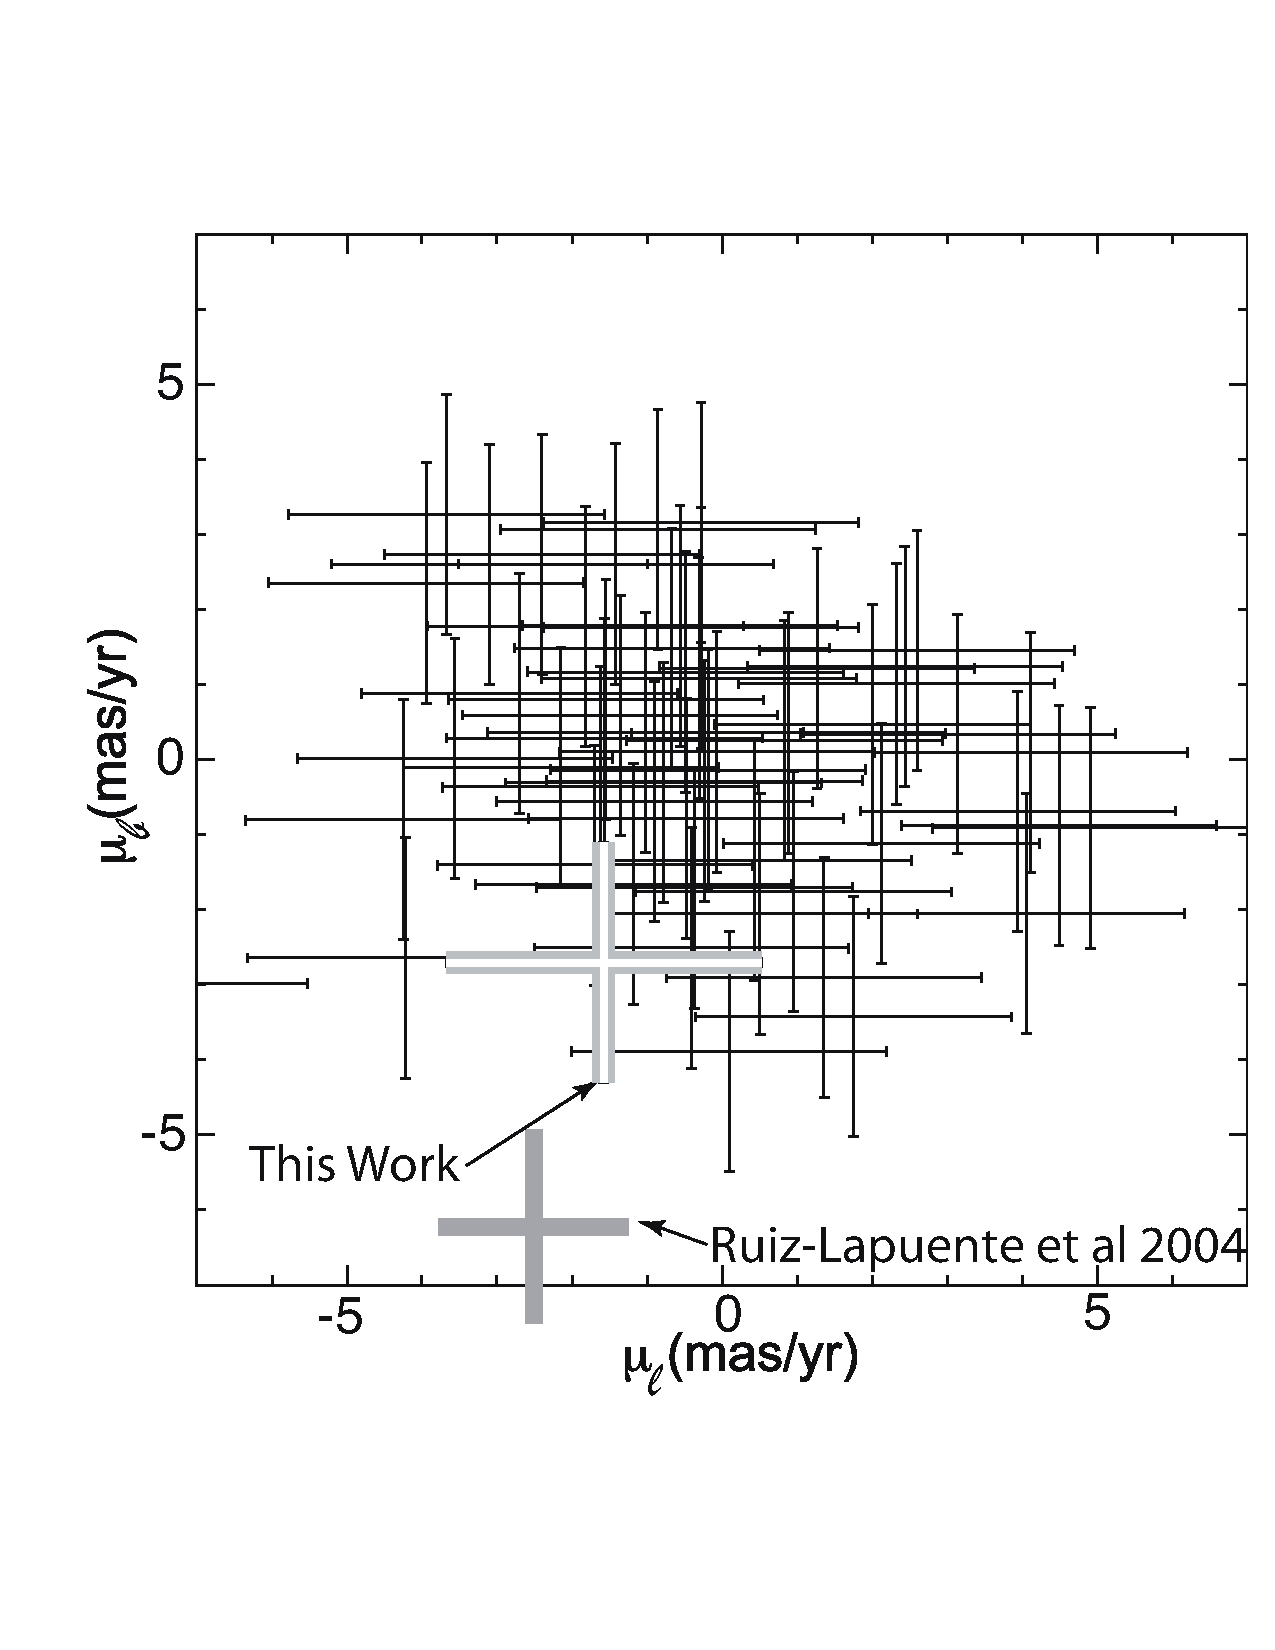
\includegraphics[width=\textwidth]{chapter_sn1572_starg/plots/prop_motion_compare_subaru.pdf}
\caption{The astrometric motions of 60 stars measured in the Tycho SNR
center. The measurements have a RMS dispersion of 1.6\,\masyr. Shown
in grey is the proper motion of \starg\ measured here and by RP04, showing a moderate discrepancy in the two measurements. Our measurement is consistent with no proper motion. }
\label{fig:prop_motion}
\end{figure}

In table \ref{tab:prop_motion} we present our astrometric measurements of all stars listed by \rl\  for which we were able to measure proper motions. We also give the apparent magnitudes in R (partly measured by this work and partly by \rl) and the distance from center $\theta$. Due to crowding caused by the relatively poor resolution of the first epoch photographic plate, several stars are not included that could be measured using \hst.
We include an  additional star, not cataloged by \rl, which exhibits high proper motion. This  high proper motion star, which was off the WFPC2 images of \rl,  we designate HP-1, and has a proper motion of $\mu_l=81.3$, $\mu_b=-2.7$ \masyr. Due to the distance from the remnant's center, (we estimate HP-1 would have been located 51$^{\prime\prime}$ from the remnant's center in 1572), we doubt this star is connected to the Tycho SN, but we include it for the sake of completeness. 

\section{Discussion}


\subsection{A Background interloper?}
\label{sec:sn1006:interloper}
A previously unrecognized property for many progenitor scenarios is the rapid post-explosion rotation of the donor (as described in Section \ref{sec:sn1572_starg_rot}).
The expected rotation as calculated in Figure \ref{fig:theorot} is
large compared to that expected of stars with a spectral type later
than F and should be easily observable. We have shown \starg's rotation to be less ($v_{\rm rot} \sin{i} \lesssim 7.5 $\,\kms) than what is expected  of an associated star if the companion was a main-sequence star or subgiant. A red giant scenario where the envelope's bloating has significantly decreased rotation could be consistent with our observation of \starg, and this will be discussed in section \ref{redgiant}.

The primary basis for which \rl\ selected \starg\ as a candidate for
the donor star to the Tycho SN was the combination of its large peculiar radial velocity
and its observed proper motion. In Figure \ref{fig:bes_d_mu} we
use the Besan\c{c}on Galactic model \citep{2003A&A...409..523R} to
construct an expected set of radial velocities for metal-rich stars in the
direction of SN1572.

\begin{figure}[htb!]
\centering
\includegraphics* [scale=0.5,angle=0]{chapter_sn1572_starg/plots/sn1572_d_vr_subaru.pdf}
\caption{Besan\c{c}on model for a metal rich ([Fe/H] $>$ -0.2 ) Galactic population between 0 and 7\,kpc in the direction of Tycho SNR (l = 120.1, b=1.4) with a solid angle of 1 square degree.
The remnant's distance is represented by the black dashed lines (as calculated in section \ref{sec:obschar}). The contours show the radial velocity distribution. 
Our measured radial velocity corrected to LSR and our distance are shown, with their respective error ranges, as the black rectangle.  The distance  range calculated by \gh\ are indicated by the two solid lines. The observed LSR $v_r$ for \starg\ is mildly unusual for stars at the remnant's distance, and is consistent with the bulk of stars behind
the remnant. }
\label{fig:bes_d_mu}
\end{figure}

Measuring the distance to \starg\ is a key discriminant in associating the star to the SN explosion. To improve the uncertainty of the distance to the star, due both to temperature and extinction uncertainty,  we base our distance on the observed $m_K$ \citep{2006AJ....131.1163S} and ($V-K$) color (\rl).  We interpolate ATLAS9 models without overshoot \citep*{1998A&A...333..231B} to find a theoretical $V-K$ and absolute magnitude for the \gh's values of temperature and gravity. Using a standard extinction law \citep*{1989ApJ...345..245C} ($A_V= 3.12 E(B-V)$ and $A_K/A_V=0.109$) to match the theoretical and observed colors, we find $A_V=2.58\pm0.08$mag, $A_K=0.28\pm 0.01$ mag, and $E(B-V)=0.84\pm0.05$.  To better show the uncertainties, we present our distance moduli scaled to the observed and derived values of extinction, temperature and gravity.
The temperature coefficients were determined by integrating blackbodies of the appropriate temperature with a filter bandpass and fitting a powerlaw to the resulting flux. \label{sec:distmod}
 
\begin{eqnarray}
(m_V-M_V)=12.93-3.12(E(B-V)-0.84)-2.5 (\log{g} -3.85)+\\
+2.5\log\left(\frac{M}{1\,M_\odot }\right)+2.5\log\left( \frac{T_{\rm{eff}}}{5900} \right)^{4.688} \nonumber\\
\label{distmodv}
(m_K-M_K)=12.93-0.275(E(B-V)-0.84)-2.5 (\log{g} - 3.85)+\\
+2.5\log\left(\frac{M}{1\,M_\odot }\right)+2.5\log\left( \frac{T_{\rm{eff}}}{5900} \right)^{1.937}\nonumber
\label{distmodk}
\end{eqnarray}

Assuming a companion mass of $1\,M_\odot$ we find a $(m-M)=12.93\pm0.75$ mag. This uncertainty is dominated by the precision of $\log{g}$, and equates to a distance of $D=3.9\pm1.6$kpc. \starg, within the errors, is at a distance consistent with the remnant.  As seen in Figure \ref{fig:bes_d_mu}, the observed radial velocity of \starg\ is consistent with a significant fraction of  stars in its allowed distance range.  We also note that if \starg\ is indeed associated with the SN, that it is likely that \starg\ could have a mass considerably less than $1\,M_\odot$, due to mass transfer and subsequent interaction with the SN, although in this case, the distance to the star would still be consistent with SNR distance. 


\citet{2007PASJ...59..811I} looked for absorption due to Fe I in the remnant's expanding ejecta for 17 stars within the Tycho remnant.  No such absorption was seen in the spectrum of \starg, potentially placing it in front of the remnant. However, the amount of Fe I currently within the remnant is uncertain with predicted column densities spanning several orders of
magnitude \citep[$0.02 - 8.9 \times 10^{15}\rm{\,cm}^{-2}$;][]{Hamilton:1988p522,Ozaki:2006p517}. Therefore, we do not believe the lack of significant Fe I 3720 absorption in \starg\ to be significant.

In summary, we find that \starg's radial velocity, distance, and stellar parameters are all consistent with an unrelated star, but also with it being the donor star. There is disagreement in  \starg's measured proper motion. The measurements of \rl\ are inconsistent with normal disk stars at the known distance and strongly point to \starg\ being associated with the SN, whereas the measurements presented here are consistent with a normal disk star, unrelated to the SN. In addition, we have shown the rotation of \starg\ is low (confirmed by \gh ; $v_{\rm{rot}} \leq 6.6$\,\kms  ), arguing against association with the SN, as does its off center placement in the remnant.  Finally, \gh\ have presented evidence that \starg\ is strongly enhanced in Nickel, an observation that, if confirmed, would strongly point to an association of the star with the SN. If either the high proper motion, or significant Nickel enhancement can be confirmed, then it is likely that \starg\ is the SN donor star. Otherwise, we believe it is much more likely that \starg\ is simply an interloper.

\subsection{\starg\ as the Donor Star to the Tycho SN}
\label{redgiant}


While the case for \starg's association with the SN is not conclusive, it is intriguing, and we believe it is worthwhile to look for a consistent solution assuming the association is true.
While not {apriori} probable, a self-consistent model can be constructed in which \starg\ was the companion, as we shall discuss now.

To make such a model work, \starg\ has to be a stripped giant that
presently mimics a G2IV star. At the time of the explosion, the star
would have been a moderately evolved giant (in a binary with an
orbital period $\sim 100\,$d). The SN ejecta will strip such a giant
of almost all of its envelope \citep{2000ApJS..128..615M} due to its low binding energy; only the most tightly bound envelope material
outside the core will remain bound. Due to the heating by the SN,
even this small amount of material (perhaps a few $\times
0.01\,M_{\odot}$) will expand to giant dimensions, and the
immediate-post-SN companion will have the appearance of a luminous red
giant. However, because of the low envelope mass, the thermal
timescale of the envelope is sufficiently short that it can loose most
of its excess thermal energy in 400 years and now have the appearance
of a G2IV star \citep{2003astro.ph..3660P}.

A lower mass for \starg\ ($0.3-0.5\,M_\odot$) also
reduces the distance estimate, and makes the observed radial velocity more unusual for stars at this distance.
The expected spatial velocity depends on the
pre-SN orbital period and should be in the range of
$30-70\,$km\,s$^{-1}$ for a period range of $20-200\,$d \citep[]{Justham:2008nx}. These velocities are consistent with the
inferred spatial velocity of the object relative to the LSR if \starg\
is at the distance of the remnant, even if no significant proper motion has been measured (see Figure \ref{fig:bes_d_mu}).

A stripped-giant companion would link the progenitor to the symbiotic
single-degenerate channel \citep{1999ApJ...522..487H} for which the
symbiotic binaries TCrB and RS Oph are well studied
candidates. Indeed, \citep[]{Justham:2008nx} argued that
the ultracool low-mass helium white dwarfs (with masses $>
0.3\,M_\odot$) that have been identified in recent years are most
likely the stripped-giant companions that survived SN Ia explosions, 
which could provide some further possible support for such a scenario for
\starg.

If the association is real, \starg's displacement to the SE of the geometric
center of the remnant as defined by radio and X-ray observations might
be interpreted as being due to the remnant's interaction with an
inhomogeneous ISM.  Deep optical images of the remnant do show
extended diffuse emission along the eastern and northeastern limbs
interpreted as shock precursor emission
\citep{2000ApJ...535..266G}. This along with an absence of detected
Balmer-dominated optical emission along the whole of the western and
southern limbs suggests a density gradient of the local interstellar
medium with increasing density towards the NE. An east-west density
gradient has also been inferred from detailed radio expansion rate
measurements \citep{1997ApJ...491..816R}.  Such an E--W density
gradient could have led to a more rapid expansion toward the west
giving rise to a small shift in the apparent geometric center away
from the SE without creating a highly distorted remnant.  However, there are problems with this explanation. Deviations from spherical symmetry in both radio and X-ray
images of the remnant are relatively small
\citep{1997ApJ...491..816R,2007ApJ...665..315C}, and the remnant is
most extended along the eastern and northeastern limbs, just where one
finds the greatest amount of extended diffuse optical
emission.
Moreover, the remnant's expansion rate appears lowest toward
the northeast (PA = 70 degrees), not the southeast \citep{1997ApJ...491..816R}. Although the
argument that \starg's SE displacement from the remnant's current
geometric center is a result of an asymmetrical expansion is not
strong, it remains a possibility.

The most conclusive way of confirming a stripped-giant scenario for
\starg\ would be an independent, precise measurement of the distance
to \starg\ which in combination with measurements of the gravity and
effective temperature would help to constrain \starg's
mass. Unfortunately, such a measurement will most likely have to wait
for the advent of the GAIA satellite.  Alternatively, one may be able
to single out a stripped giant from a normal G2IV star through
nucleosynthesis signatures, specifically evidence for CNO-processed
material (or other nucleosynthetic anomalies).  While a normal G2IV star is unlikely to show CNO-processed
material at the surface, a stripped giant is likely to do so. Unfortunately, the data presented here are not of adequate quality to explore the detailed properties of \starg's atmosphere.

\section{Outlook and Future Observations}

Presently, we believe the evidence for \starg's association with the Tycho SN is interesting, but not conclusive.
A possible scenario if \starg\ is the donor star, would be that of a stripped giant scenario discussed in section 6.  
However, there are still other stars that have not been adequately
scrutinized. \citet{2007PASJ...59..811I} have found a star (\rl\
Star-E) which may contain blueshifted Fe I lines, indicating their
association with the remnant. Unfortunately, the star has neither
a significant peculiar radial velocity (\citealt{2007PASJ...59..811I}; \rl)
 nor a significant peculiar proper motion (\rl\ and confirmed by
our work; see Table \ref{tab:prop_motion}).

High-resolution spectroscopy of each candidate in the remnant's center is necessary to
precisely determine each star's physical parameters. However, the small observed
velocities of the remaining stars suggest that the donor star would
have needed to be a giant at the time of explosion. Using \rl's
observed values, none of the stars in the remnant's center appear
consistent with what is expected of a giant star as the donor star
except possibly for Star-A.  We also note that there is an additional
star present in archived HST images, not cataloged in \rl, offset from \rl's star A  by
0.5$^{\prime\prime}$ E and 0.2$^{\prime\prime}$ N at $m_V=16.8$,
$(B-V)=1.0$. This star, near the remnant's centre, has a color
consistent with an F-star (assuming that it is behind the bulk of the
line of sight reddening), but it will require adaptive optics to
obtain its spectrum given its proximity to the 13th magnitude Star-A. This star could potentially be a non-giant
progenitor.

If future observations are unable to pinpoint a viable donor star,
other progenitor scenarios will have to be considered. These include
the double degenerate scenario, or a scenario where there is a long
time delay between the accretion phase of a donor star onto the white dwarf, and the ultimate supernova
explosion.

\bigskip
We would like to thank the Subaru HDS team for taking these
observations in service mode. This paper makes use of data obtained
from the Isaac Newton Group Archive which is maintained as part of the
CASU Astronomical Data Centre at the Institute of Astronomy,
Cambridge. This publication makes use of data products from the Two
Micron All Sky Survey, which is a joint project of the University of
Massachusetts and the Infrared Processing and Analysis
Center/California Institute of Technology, funded by the National
Aeronautics and Space Administration and the National Science
Foundation. This work also makes use of POSS-I data. The National Geographic Society - Palomar Observatory Sky Atlas (POSS-I) was made by the California Institute of Technology with grants from the National Geographic Society. 
WEK, BPS and MA are supported by the Australian Research
Council (grant numbers DP0559024, FF0561481). This paper was conceived as part of the Tokyo Think Tank
collaboration, and was supported in part by the National Science
Foundation under Grant No. PHY05-51164.
This work was supported in part by World Premier International
Research Center Initiative (WPI Program), MEXT, Japan, and by the
Grant-in-Aid for Scientific Research of the Japan Society for the
Promotion of Science (18104003, 18540231, 20540226) and MEXT (19047004, 20040004). 
Additionaly we would like to thank Pilar Ruiz Lapuente and her team for the valuable discussions we had in regards to the manuscript. We would also like to thank our referee, who provided us with a very detailed and thorough analysis of the first manuscript and subsequent revisions. 

% !TEX root =single_chapter_sn1572_hires.tex
%% !TEX root = ../thesis.tex
\chapter{Tycho's Six: High-Resolution spectroscopy search for the remaining donor for the Tycho supernova}
\label{chap:sn1572_hires}

% TITLE AND AUTHORS
%-----------
%\title{Tycho's Six: High-Resolution spectroscopy search for the remaining donor for the Tycho supernova\footnotemark{1}}

\section{Introduction}
\label{sec:introduction}

Type Ia Supernovae (\sneia) are of great interest for astronomy. They represent some of the most extreme physical situations in stellar astronomy, produce substantive amounts of Iron group elements which impacts the chemical evolution of galaxies and the Universe, and are uniquely powerful probes of Cosmic distance.
applications in stellar and galactic astronomy as well as in cosmology. Despite their wide ranging significance, fundamental uncertainties remain around  progenitor of these cataclysmic events. 

There is general consensus that \sneia\ are caused by the deflagration/detonation of a Carbon/Oxygen white dwarf which is accreting material from a binary companion. Scenarios exists where the explosion can be initiated from a detonation on the surface of the star (reference of Livne, and Sim), through runaway carbon burning in the white dwarfs interior, or through a cataclysmic merger of objects.

Observationally, two main scenarios for this accretion process can be identified.. The first scenario sees the accretion process occurring through Roche Lobe Overflow (henceforth RLOF) of a close non-degenerate companion (also known as donor star). This companion, which has undergone common envelope evolution with the white dwarf, can be a helium, main-sequence, sub-giant, or red giant star. is a main-sequence to red giant star at the time of the explosion (\sd\ scenario). In all cases the donor star should survive the explosion and remains visible post-explosion.

The second scenario is the  dynamical merger of two white dwarfs (\dd\ scenario). In this scenario, the co-evolution of two stars eventually leads to a close binary of two white dwarfs, which are able, through the emission of gravitational radiation, to merge over a wide range of times after the initial formation of the system. In most cases this would leave no remaining star \citep[e.g.][]{2010Natur.463...61P}.

Both scenarios have support in observation and theory. The detection of circum-stellar material around certain SN Ia, such as SN 2006X \citep{2007Sci...317..924P}, provides support for the \sd\ model. On the other hand the lack of substantial hydrogen in in the majority of other \sneia\ \citep{2007ApJ...670.1275L} poses a challenge to the \sd\ scenario.


\citet{2010ApJ...708.1025K} suggests that the interaction with the non-degenerate companion should imprint an observable signature on a SN Ia  light curve, depending on viewing angle, and radius of the companion. Such an excess has not yet been observed \citep{2010ApJ...722.1691H, 2011Ap&SS.tmp...40T, 2011arXiv1106.4008B}.which is at odds with Red Giant companions forming the majority of \sneia.


Population synthesis calculations are challenging, with various authors getting different results for the same inputs (Nelemans paper). However there is a general trend from these calculations that neither single-degenerate nor double degenerate stars can provide enough systems to explain the SN Ia rate \citep{2009ApJ...699.2026R, 2010A&A...515A..89M,2010A&A...521A..85Y,2008ApJ...677L.109H}. Several authors suggest the population might comprise both single and double degenerate systems.

The physics of white dwarf mergers is challenging to numerically simulate, but in the simplest calculations, these mergers will lead to the formation of a neutron star \citep{1985A&A...150L..21S}. Recently \citet{2010Natur.463...61P} have shown that for certain parameters (white dwarf binaries with a mass ratio very close to one) the merger may explain sub-luminous supernovae. 

To investigate the nature of progenitors observationally \citet[][henceforth \rl]{2004Natur.431.1069R} have tried to directly detect donor stars in \snia\ remnants within the Milky Way. They have identified two historical Galactic SN well suited to this task - SN 1006 and Tycho's SN (SNR1572 henceforth). Both remnants are young (440 and 1000 years old, respectively), almost certainly SN Ia from both their observational signatures (RP 04 but not RP04), Badenes et al. (look it up), and not overwhelmed by Galactic extinciton. In this paper, we will focus on SN1572. 

SNR1572 is relatively close ($2.8\pm0.8$\,kpc), very young and has been confirmed as a normal \snia\ remnant \citep{2006ApJ...645.1373B, 2008Natur.456..617K}.  While the star has an unusual spatial motion compared to other stars in the field, its current location and proper motion place it a significant distance from the remnants center - a feature difficult to explain in connecting \starg\ to SNR1572.

\rl\ investigated most bright stars in the central regions of SN1572 and found a star with an unusual spatial motion (\starg\ by their nomenclature) and suggested this as a possible donor star for SN1572. 
One consequence of RLOF is a rotational velocity induced on the donor star by tidal locking in the system. This results in an unusually large rotationally velocity, related to the orbital velocity of the binary system and can be used to single out donor stars against nearby unrelated stars. \citep[][,henceforth \wek]{2009ApJ...701.1665K} investigated rotation for  \starg\ but found no excess rotation velocity compared to a normal star. \wek's measurements of \starg, including a revised radial velocity, compared to a Galactic models, showed it is statistically consistent with an interloping star. However, \wek\ were able to provide an a priori unlikely scenario, where the star was able to lose its rotational signature. 

\citet[henceforth \gh]{2009ApJ...691....1H} analysed a spectrum of \starg\ observed with the HIRES-instrument on the Keck telescope. \gh confirmed \wek's radial velocity for \starg\ and determined its stellar parameters and metallicities. \gh in addition to refining the metallicity, Temperature and Gravity measurements for \starg, concluded concluded that \starg\ has an unusually large amount of Ni. \gh\ claim that this Ni measurement could be attributed to the accretion of ejecta material on the donor star. 

In this paper we analyse HIRES spectra of the 6 bright stars in SNR1572 center. These spectra were taken by the same program that obtained the data used by GH-09, and we independently reanalyze this spectrum as part of our program.

We describe the observational data and our data reduction procedures in Section \ref{sec:observ-data-reduct}. Section \ref{sec:analysis} is divided into five subsections detailing the measurements of proper motion, radial velocity, rotation, stellar parameters and abundances. In Section \ref{sec:discussion} we analyse the measurements of each star to investigate its potential association with SNR1572, and present our conclusion in section \ref{sec:conclusion}.

\section{Observations and Data Reduction}
\label{sec:observ-data-reduct}

We obtained spectra with the High Resolution Echelle Spectrograph \citep[HIRES][]{1994SPIE.2198..362V} on the Keck 10m telescope in Mauna Kea. The observations were made on two nights on 2006 September 10 and 2006 October 11.  The slits B5 and C1 (with the same width of 0.86\arcsec\ but different lengths, B5 length 3.5\arcsec, C1 length 7.0\arcsec) were used resulting in a wavelength coverage of 3930 -- 5330 \AA, 5380 -- 6920 \AA\ and 6980 -- 8560 \AA\ with $R\approx 50,000$, providing us with the necessary spectral resolution and wavelength coverage to determine stellar parameters. 
The spectra were reduced using the MAKEE package. All spectra were corrected to heliocentric velocities, using the MAKEE skyline method. The spectra were not corrected for telluric lines as they will not influence our analysis of the stellar parameters. The final exposure times of the combined spectra for each candidate and signal to noise ratio at 4000-4100 \AA\ are shown in Table \ref{tab:candexpo}. Finally we normalized the spectrum using the IRAF-Task continuum. We note that \starc\ and \stard\ were observed on the same slit (C1) with a separation of 2.1\arcsec.

\ctable[
% 
caption = {Observations of Stars},
% 
label = {tab:candexpo},
%
%
]{lcccccc}{}{ \FL
Name & RA (J2000) & Dec (J2000)  & Date & Slit & $t_{\rm exp}$& S/N \\
designation & (hh:mm:ss.ss) & (dd:mm:ss.ss) & (dd/mm/yy) &  & (s) &  \ML
%
%Now the data...
\stara & 00:25:19.73 & +64:08:19.6 & 10/09/06 & B5& 900 &$ \approx 65$ \\
\starb & 00:25:19.95 & +64:08:17.11 & 10/09/06 & B5 & 1200 &$ \approx 50$ \\ 
\starc & 00:25:20.40 & +64:08:12.32 & 11/10/06 & C1 &  10800 & $ \approx 10$\\ 
\stard & 00:25:20.60 & +64:08:10.82 & 11/10/06 & C1 & 10800 & $ \approx 5$ \\
\stare & 00:25:18.29 & +64:08:16.12 & 11/10/06 & C1 & 9000 & $\approx 15$\\ 
\starg & 00:25:23.58 & +64:08:02.06 & 10/09/06 \& 11/10/06  & B5\&C1 & 24000 & $\approx 30$ 
\LL}


In addition, we obtained low-resolution spectroscopy ($R\approx1200$) of
\starb\ with the dual-arm Low-Resolution Imaging Spectrometer \citep[LRIS;][]{Oke95} mounted on the 10-m Keck I telescope. The
observations were taken on one run on 2010 November 07, using only the blue
arm with the 600/4000 grism and the 1\arcsec\ wide slit. This resulted
in a wavelength coverage of 3200 -- 5600\,\AA. These observations
were taken to obtain a precise  measurement of the surface gravity for \starb\ using the size of the Balmer decrement.
The spectrum of \starb\ was reduced using standard techniques \citep[e.g.][]{Foley03}. Routine CCD processing and spectrum extraction
were completed with IRAF\footnote{IRAF: the Image Reduction and
Analysis Facility is distributed by the National Optical Astronomy
Observatory, which is operated by the Association of Universities for
Research in Astronomy (AURA) under cooperative agreement with the
National Science Foundation (NSF).}, and the data were extracted with
the optimal algorithm of \citet{Horne86}. We obtained the wavelength
scale from low-order polynomial fits to calibration-lamp spectra.
Small wavelength shifts were then applied to the data after measuring the offset by
cross-correlating a template sky to the night-sky lines that were
extracted with the star. Using our own IDL routines, we fit a
spectrophotometric standard-star spectrum to the data in order to flux
calibrate \starb\ and remove telluric lines \citep{Horne86,Matheson00}.


\section{Analysis}
\label{sec:analysis}

\subsection{Astrometry}
\label{sec:propmot}
Proper motions can be used to identify potential donor stars because donor stars freely travel with their orbital velocity after the SN explosion disrupts the system. \rl\ suggested \starg\ as a possible donor due to its unusually high proper motion and unusually high radial velocity. For this work we measured proper motions for 201 stars within one arcminute of the remnant's center. We used archival HST images for three different epochs (HST Program ID  9729 \& 10098; November 2003, August 2004, May 2005) each consisting of three exposures (1\,s, 30\,s and 1440\,s) in the F555W using the Advance Camera for Surveys (ACS). The pixel size in each exposure is 50\,mas\,pixel$^{-1}$. This dataset results in a maximum baseline of 30 months. 


We used an image from the middle epoch (2004) to establish a reference frame and oriented the pixel coordinate system with the equatorial system. We then applied a distortion correction for the F555W filter \citep{2006acs..rept....1A} to each images and then calculated transformations (order xxxxx) between all other images and the reference image. We then used these transformations to calculate the position of all stars in the reference coordinate system  with the overall uncertainty of each position estimated (How?).
Some faint stars where not detected in the shorter exposures and were thus excluded from proper motion measurements (with 114 Stars remaining).

For each star, we fit a linear regression for the stellar positions over time in the pixel coordinates (which were aligned with the equatorial system). The x and y data were treated as independent measurements, with separate regressions solved for each axis directions. Errors were estimate using standard least squares analysis and the individual error estimates each object's positions.

There are three measurements of the geometric center of SN1572 using different datasets. \cite{1997ApJ...491..816R} using VLA data determined the center to R.A. 00:25:14.95 Dec +64:08:05.7 J2000,  \citet{2000ApJ...545L..53H} using ROSAT data got R.A. 00:25:19 Dec +64:08:10 J2000 and \cite{2005ApJ...634..376W} with Chandra data determined the center to R.A. 00:25:19.40 Dec +64:08:13.98 J2000. 

 Table \ref{tab:propmot} lists the proper motions and errors of all stars mentioned in \rl\ (19 stars) which were analyzed in this work as well as the distance to the geometric X-Ray center measured by Chandra.

We compared the distribution of proper motions of all measured stars to ours candidates in Figure \ref{fig:propmot_sn1572_hires}.

\ctable[
caption = {Proper motion of Candidates},
label = {tab:propmot},
]
{lccccccc}{}{\FL
%
Name & RA (J2000) & Dec (J2000) & $\mu_\alpha$ & $\mu_\delta$ & $\Delta\mu_\alpha$ & $\Delta\mu_\delta$ & $r$\\
designation & (hh:mm:ss.ss) & (dd:mm:ss.s) & \masyr & \masyr & \masyr & \masyr \arcsec \ML
%\startdata
B & 0:25:19.97 & 64:08:17.1 & -1.24 & 0.56 & 0.62 & 0.64 & 4.86\\
A & 0:25:19.73 & 64:08:19.8 & -0.09 & -0.89 & 1.17 & 0.90 & 6.21\\
A2 & 0:25:19.81 & 64:08:20.0 & -0.71 & -3.60 & 0.69 & 0.64 & 6.58\\
C & 0:25:20.38 & 64:08:12.2 & -0.21 & -2.52 & 0.65 & 0.65 & 6.66\\
E & 0:25:18.28 & 64:08:16.1 & 2.04 & 0.54 & 0.66 & 0.69 & 7.60\\
D & 0:25:20.62 & 64:08:10.8 & -1.12 & -1.99 & 1.01 & 0.86 & 8.60\\
1 & 0:25:16.66 & 64:08:12.5 & -2.27 & -1.37 & 1.60 & 1.15 & 18.00\\
F & 0:25:17.09 & 64:08:30.9 & -4.41 & 0.20 & 0.70 & 0.71 & 22.69\\
J & 0:25:15.08 & 64:08:05.9 & -2.40 & -0.25 & 0.62 & 0.62 & 29.44\\
G & 0:25:23.58 & 64:08:01.9 & -2.50 & -4.22 & 0.60 & 0.60 & 29.87\\
R & 0:25:15.51 & 64:08:35.4 & 0.28 & 0.24 & 0.89 & 0.80 & 33.23\\
N & 0:25:14.73 & 64:08:28.1 & 1.18 & 0.89 & 0.86 & 0.98 & 33.66\\
U & 0:25:19.24 & 64:07:37.9 & 0.01 & -3.04 & 0.73 & 0.75 & 36.06\\
Q & 0:25:14.81 & 64:08:34.2 & 1.45 & 3.07 & 0.64 & 0.72 & 36.19\\
T & 0:25:14.58 & 64:07:55.0 & -3.85 & 0.52 & 0.72 & 0.62 & 36.78\\
K & 0:25:23.89 & 64:08:39.3 & 0.18 & 0.17 & 0.73 & 0.69 & 38.73\\
L & 0:25:24.30 & 64:08:40.5 & 0.16 & -0.44 & 0.75 & 0.82 & 41.59\\
S & 0:25:13.78 & 64:08:34.4 & 4.16 & 0.58 & 0.83 & 0.84 & 42.09\\
2 & 0:25:22.44 & 64:07:32.4 & 74.85 & -4.43 & 0.82 & 0.83 & 46.09\\
%\enddata
\LL}


\begin{figure}[htbp] % figure placement: here, top, bottom, or page
   \centering
   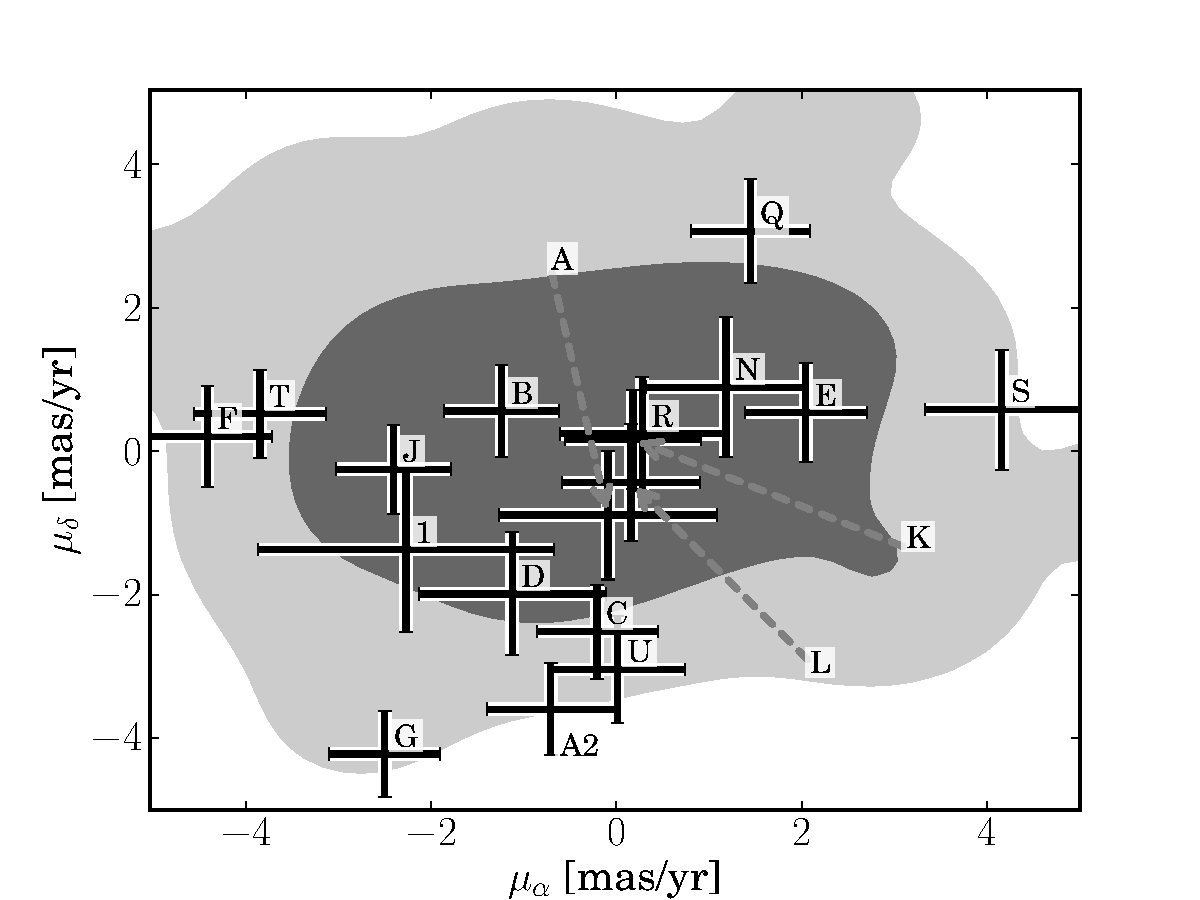
\includegraphics[width=0.5\textwidth]{chapter_sn1572_hires/plots/propmot_distr.pdf}
   \caption{The contours show the distribution of proper motion ($1-\sigma$ and $2-\sigma$) excluding the named stars.
    We show the location of the candidate stars and their errors on top of this distribution. Tycho-2 was not shown in this figure as it is an extreme outlier with $\mu_\alpha=75$\,\masyr\ and $\mu_\delta=-4.4$\,\masyr\ but also at a large distance to the center of the remnant's geometric center (46\arcsec).}
   \label{fig:propmot_sn1572_hires}
\end{figure}


\subsection{Radial Velocity}
\label{sec:radvel}

The radial velocity of each star was measured using the IRAF task \textit{fxcor} \citep{1979AJ.....84.1511T}. MAKEE was used to calculate an intrinsic velocity shift by comparing offsets of the nightsky-lines. The radial velocity standards were reduced in the same fashion. 
 
Each order of each star was then cross-correlated with at least two other radial velocity standards (HR6349, HR6970, HR1283) which had been observed on the same night.


The radial velocity for \starb\ was measured in the course of determining the stellar parameters for \starb\ with the stellar parameter fitting package \textit{sfit} \citesfit. The \textit{sfit} result consistently gives $v_{\textnormal{helio}} = -55$ \kms\ for different stellar parameters with an error of $\approx 2$\,\kms. 


In Table \ref{tab:radvel} we have listed all the radial velocities both in a heliocentric frame and a local-standard-of-rest (henceforth LSR) frame. We will be referring to the heliocentric measurements from here on. The listed error is the standard deviation of the radial velocity measurement of all orders added in quadrature to the error of the radial velocity standards.

In Figure \ref{fig:dist_vr} we have compared the radial velocity of our sample stars to radial velocities of stars in the direction of Tycho's SNR using the Besan\c{c}on Model \citep{2003A&A...409..523R}. The distance as well as the error in distance are taken from Section \ref{sec:distance}.  The candidates radial velocities are all typical for their distance. Finally, we note the measurement of \starg\ is consistent with \wek\ and \gh.

\ctable[
caption = {Radial velocities},
label = {tab:radvel},
]
{lccccc}{}{\FL
Name & Date & $v_{\rm helio}$ & $v_{\rm LSR}$ &$\Delta v$ \\
designation & (dd/mm/yy) & (\kms) & (\kms) & (\kms) \ML
%startdata
\stara & 09/09/06 & -36.79 & -28.5 & 0.23   \\
\starb & 09/09/06 & -55.0 & -57.0 & $\approx 2$ \\
\starc & 11/10/06 & -58.78 & -50.49 & 0.75   \\
\stard & 11/10/06 & -58.93 & -50.64 & 0.78   \\
\stare & 11/10/06 & -64.2 & -55.91 & 0.27   \\
\starg & 09/09/06 & -87.12 & -78.83 & 0.25 \\
\starg & 11/10/06 & -87.51 & -79.22 & 0.78 
\LL
}

\begin{figure}[htbp] %  figure placement: here, top, bottom, or page
   \centering
   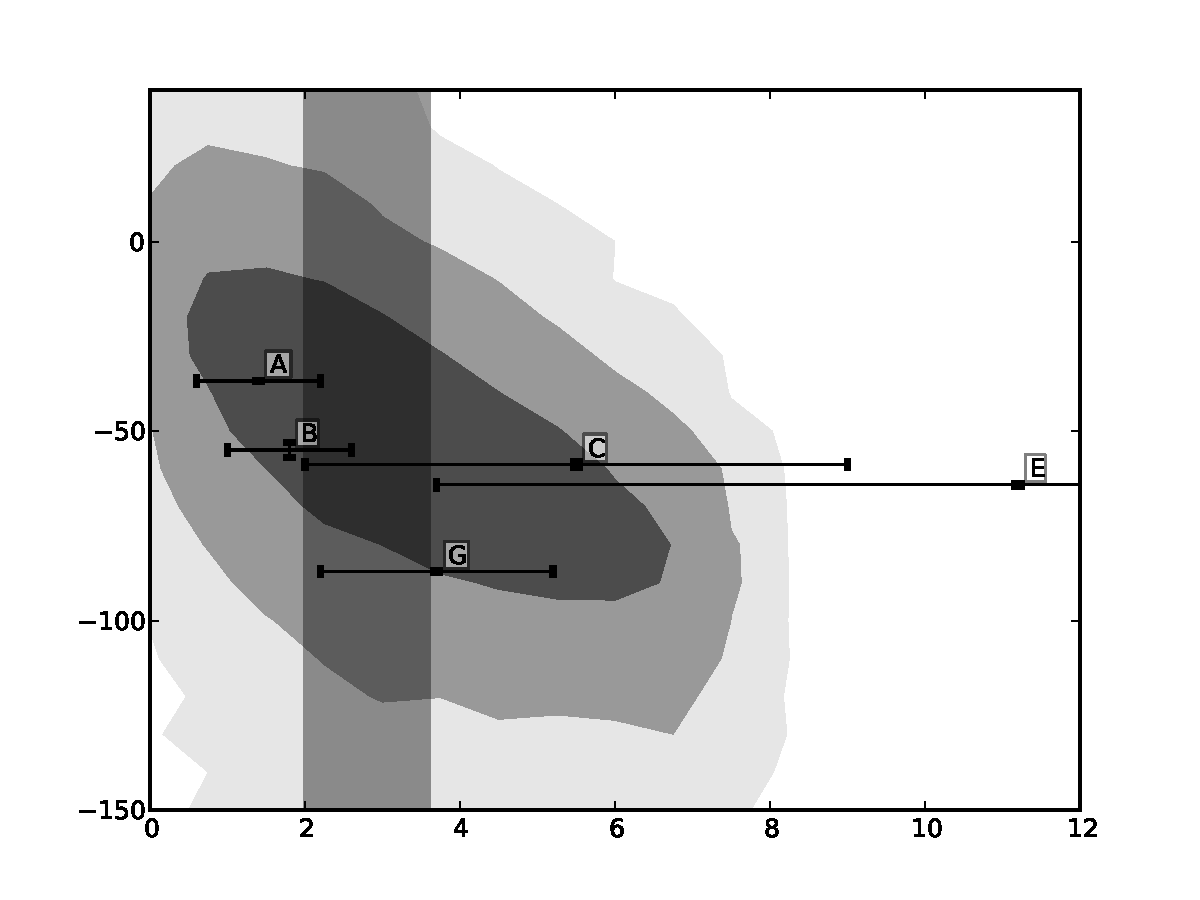
\includegraphics[width=0.5\textwidth]{chapter_sn1572_hires/plots/dist_vr.pdf} 
   \caption{The contours indicate 1, 2 and $3-\sigma$ levels of the distance and radial velocity using the Besan\c{c}on Model \citep{2003A&A...409..523R} with $\approx 60 000$ stars in the direction of SNR1572 (only including star with a V between 10 and 20 as well as stars with a metallicity of [Fe/H] $> -1$). We have overplotted our candidate stars with error bars. One should note that the errors in distance are only an indication of the error, the proper error surfaces can be seen in Figure \ref{fig:mc_isochrone}. The vertical gray shade shows the error range for the distance of SNR1572.}
   \label{fig:dist_vr}
\end{figure}



\subsection{Rotational Velocity}
\label{sec:rotation}
We have measured rotational velocities of all stars except \starb\ in the same fashion as described in \wek. We selected several unblended and strong (but not saturated) \ion{Fe}{1} lines in the stellar spectra .  We added these lines after shifting them to the same wavelength and scaling them to the same equivalent width. This was done to improve the signal to noise ratio for the faint stars as well as providing consistency throughout all stars. 

 As a reference we created three synthetic spectra for each star (one broadened only with the instrumental profile, the others with the instrumental profile and $v_{\rm{rot}}\sin{i}$\ of 10 and 13\,\kms\ respectively) with the 2010 version of MOOG \citemoog, using our derived temperature, gravity and metallicity.  As input data to MOOG we used the \citet{2004astro.ph..5087C} atmospheric models and a line list from \citet{1995KurCD..23.....K}. We then applied the same process of line selection and adding as for the lines in the observed spectra. 
 
Figure \ref{fig:rotvel} shows the comparison between the synthetic spectra of different rotational velocity and the observed spectra. This comparison indicates that the stellar broadening (rotational, macro turbulence, etc. ) is less than broadening due to the instrumental profile of 6\,\kms\ for each star. We adopt 6\,\kms\ as an upper limit to the rotation for all stars.



\begin{figure*}[h!]
\begin{tabular}{cc}
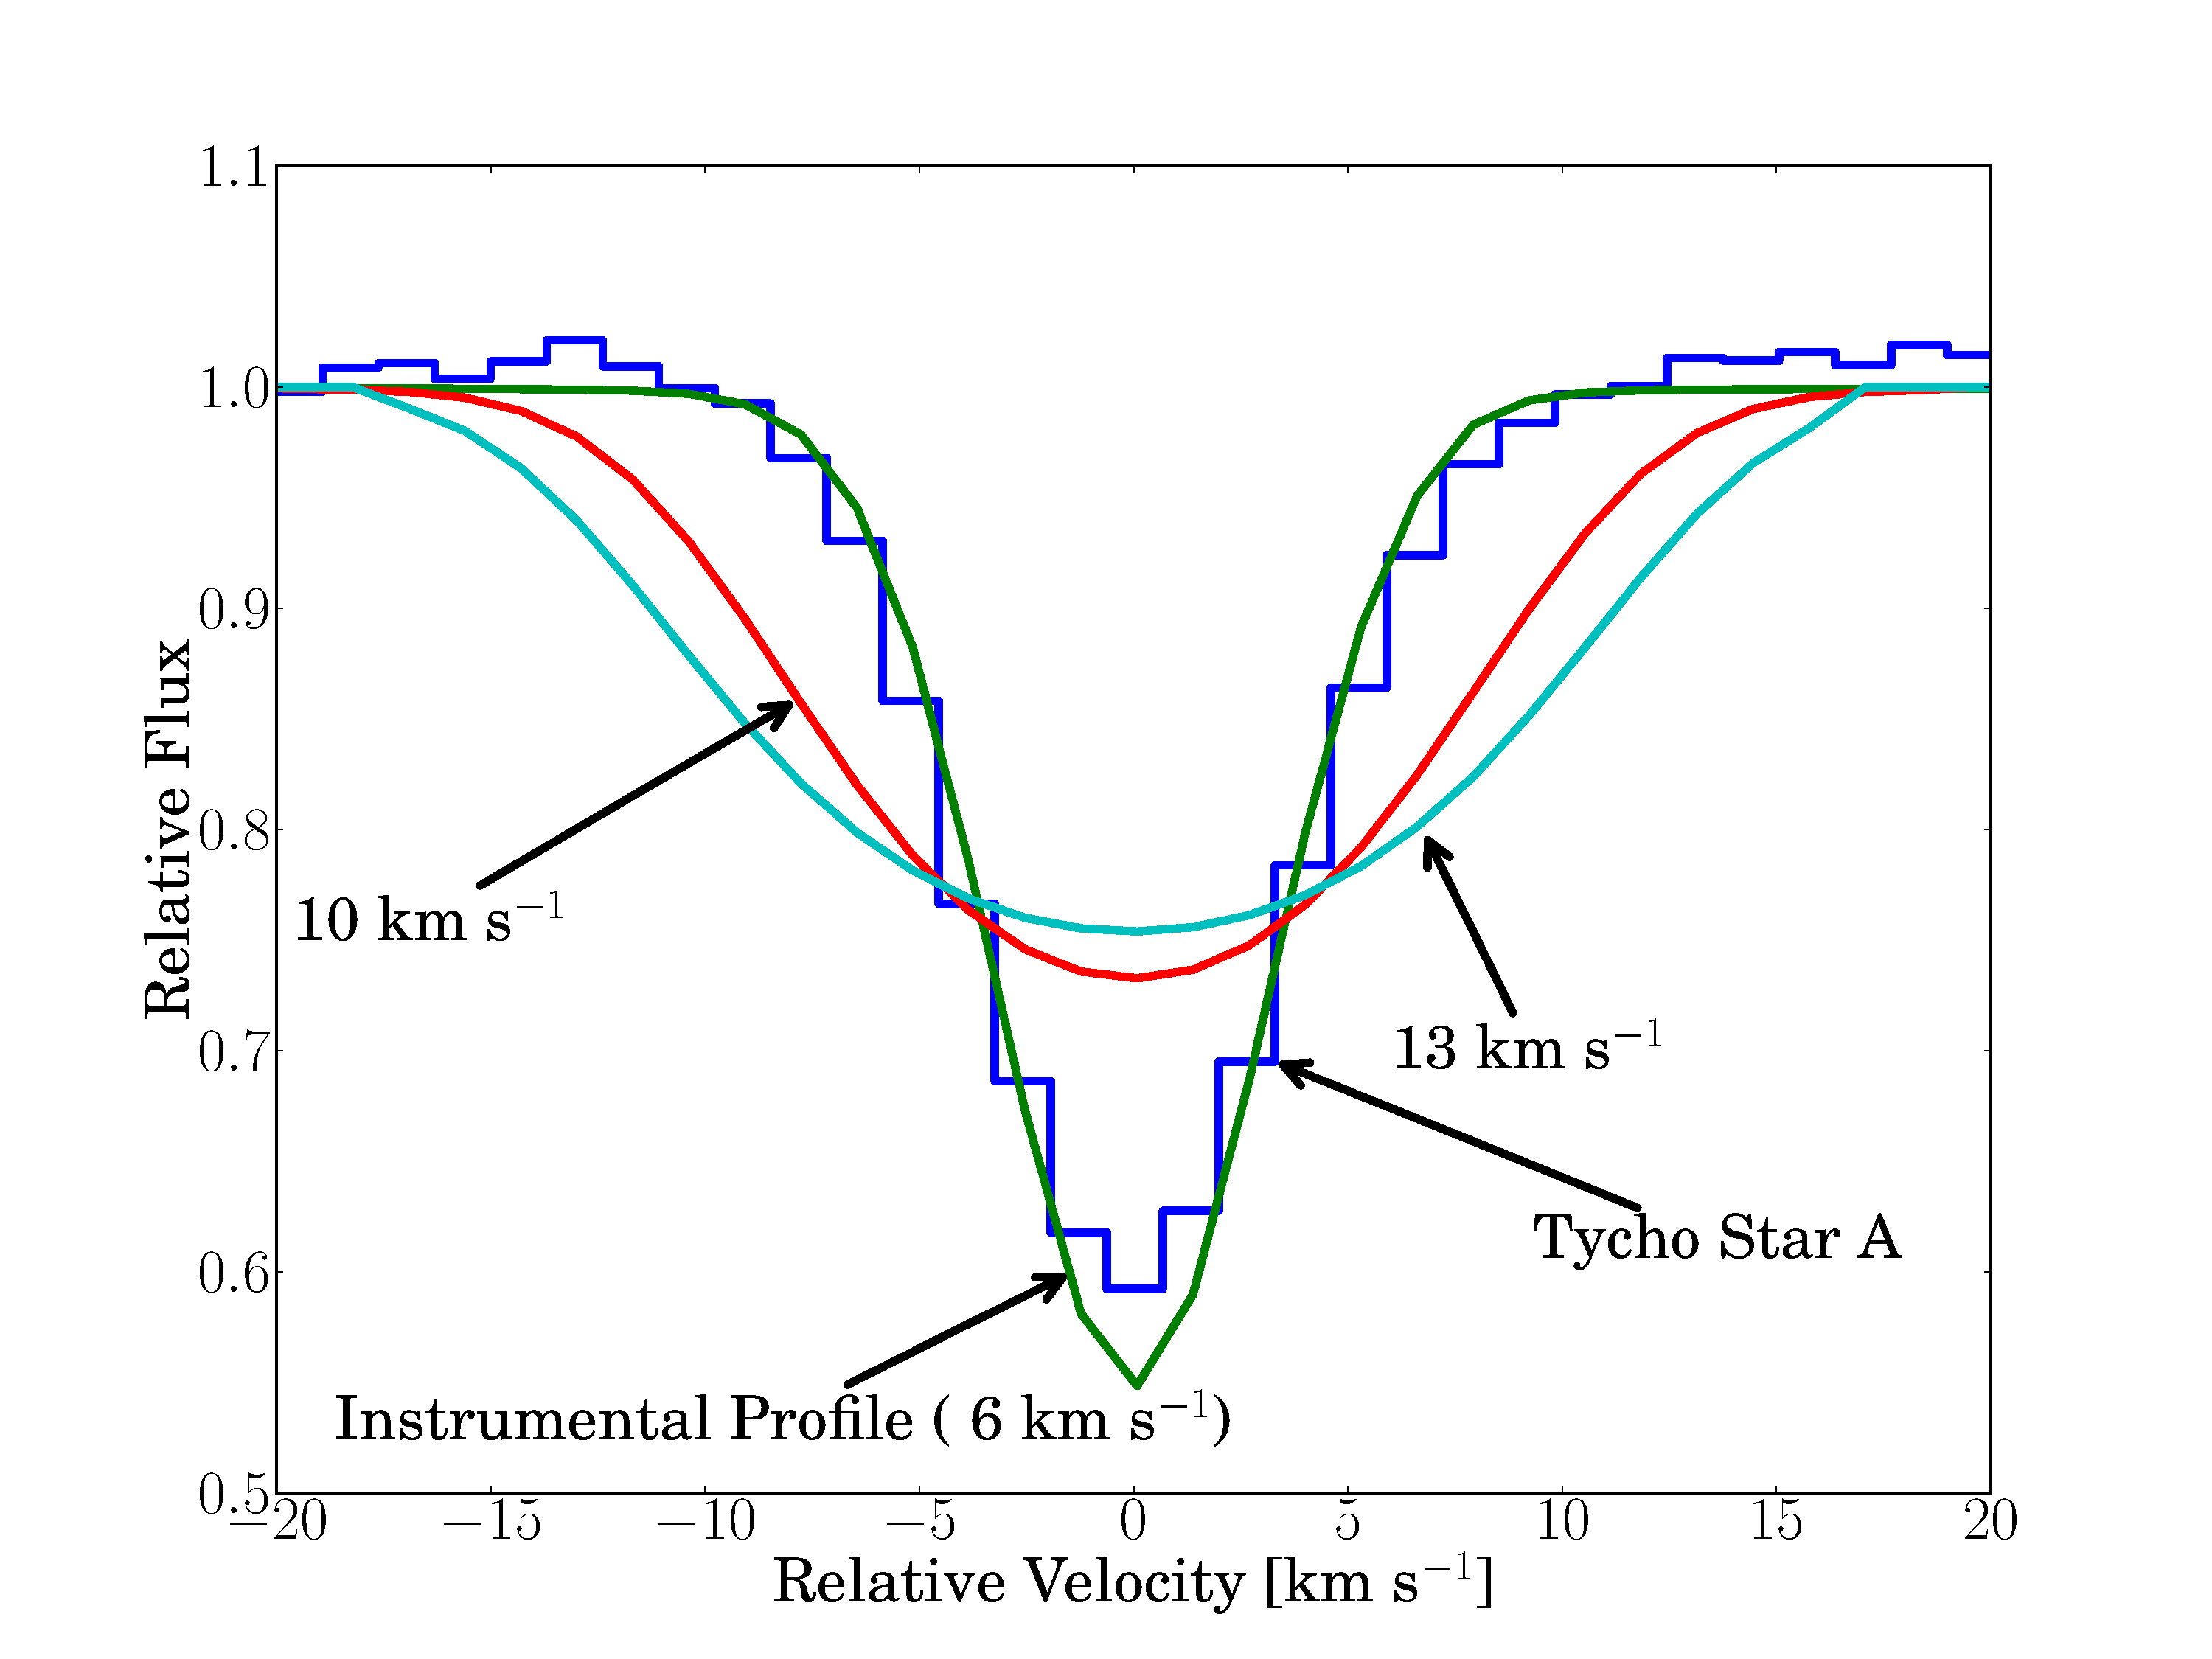
\includegraphics[width=0.45\textwidth, trim=130 30 60 0]{chapter_sn1572_hires/plots/stara_rotation.pdf} &
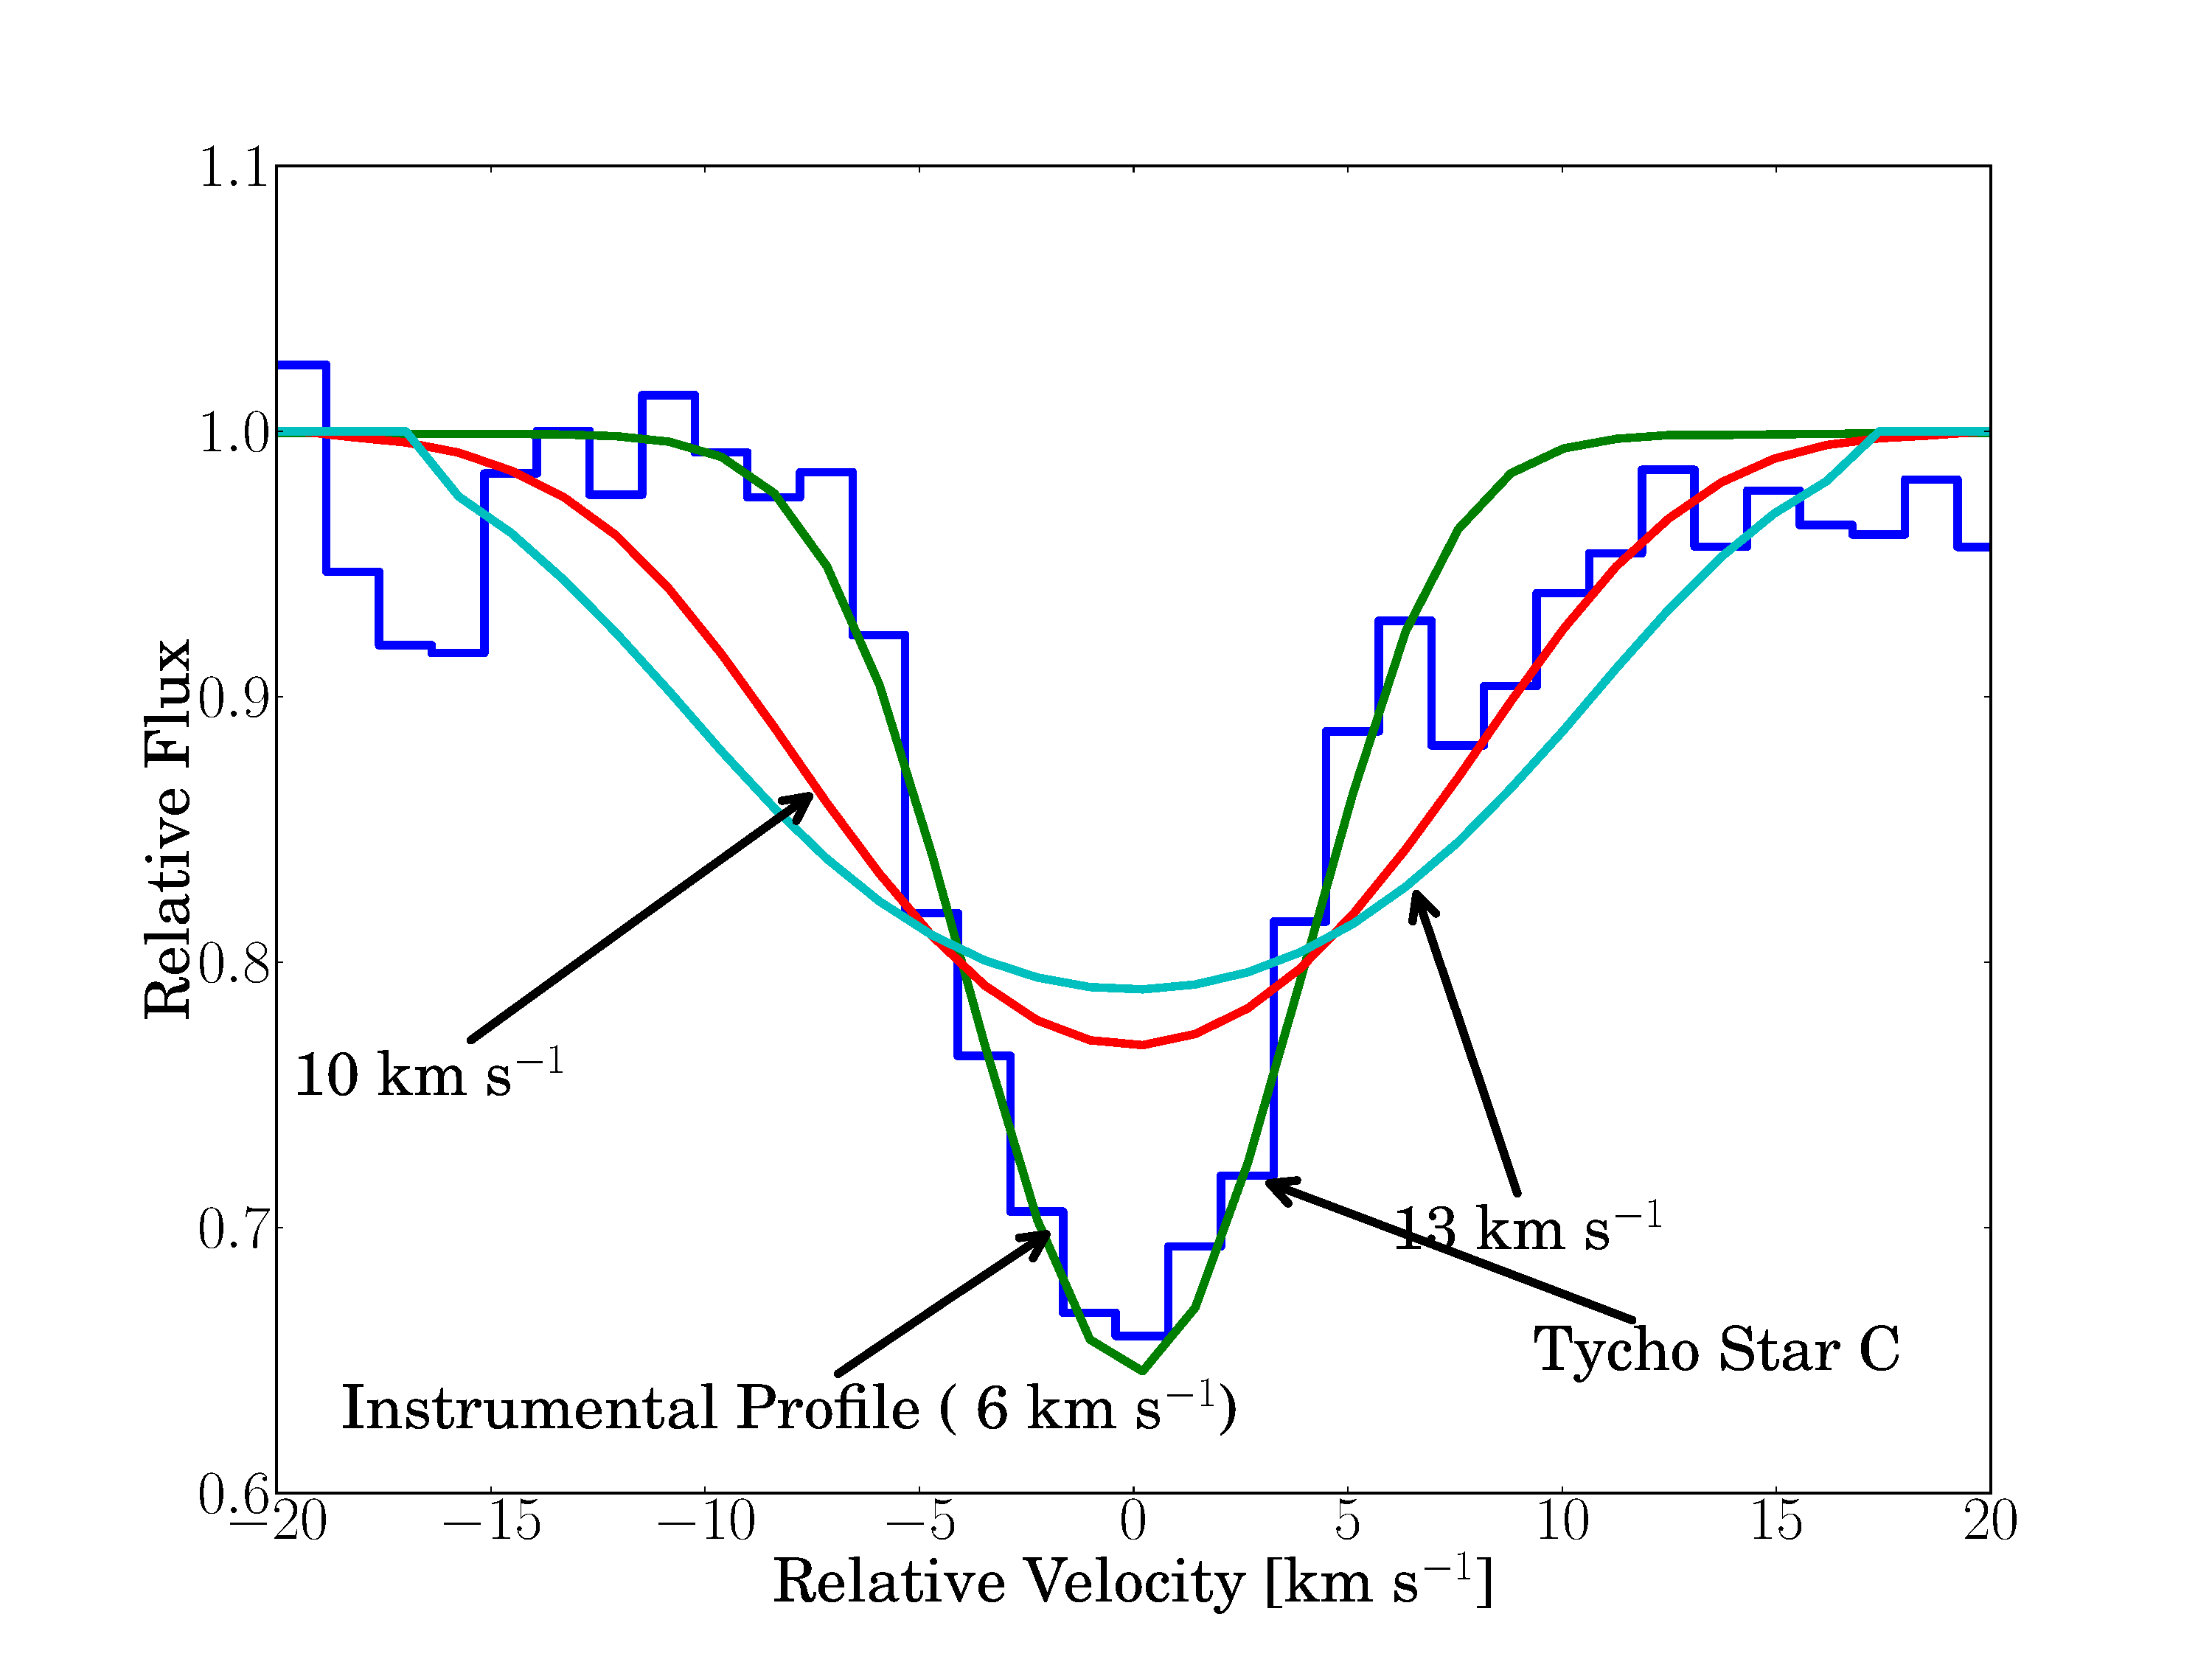
\includegraphics[width=0.45\textwidth, trim=130 30 60 0]{chapter_sn1572_hires/plots/starc_rotation.pdf} \\
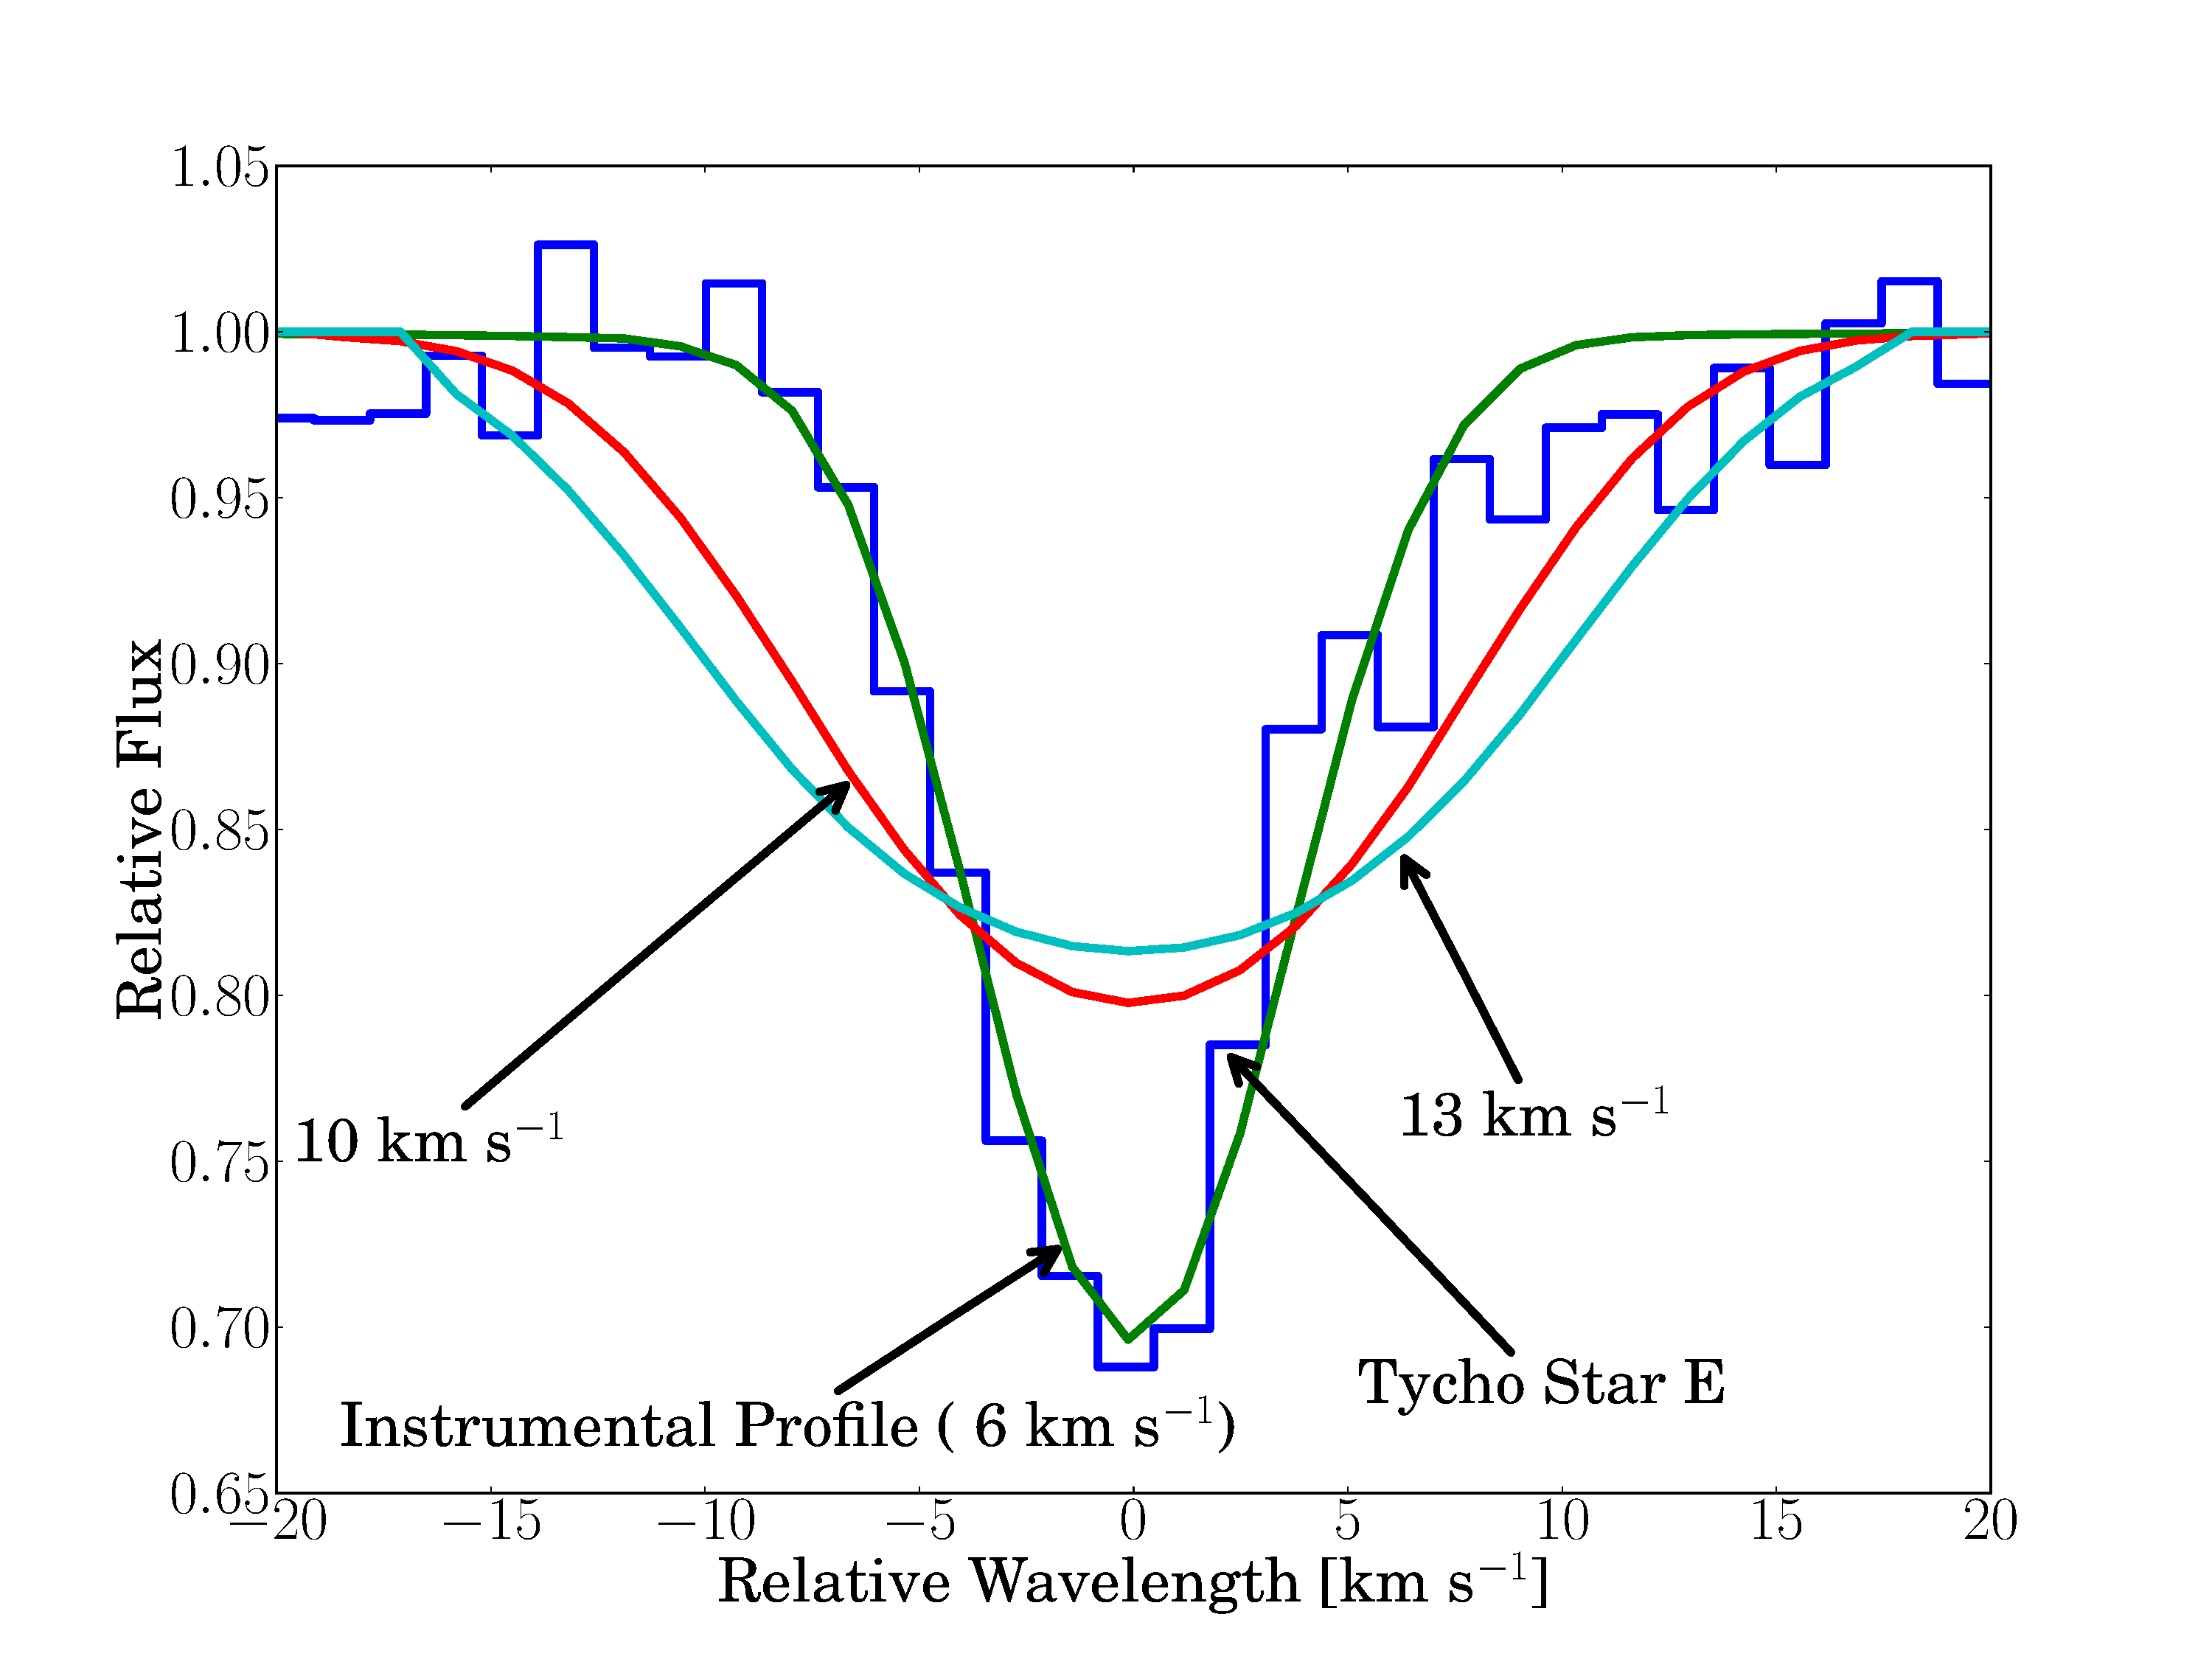
\includegraphics[width=0.45\textwidth, trim=130 30 60 0]{chapter_sn1572_hires/plots/stare_rotation.pdf} &
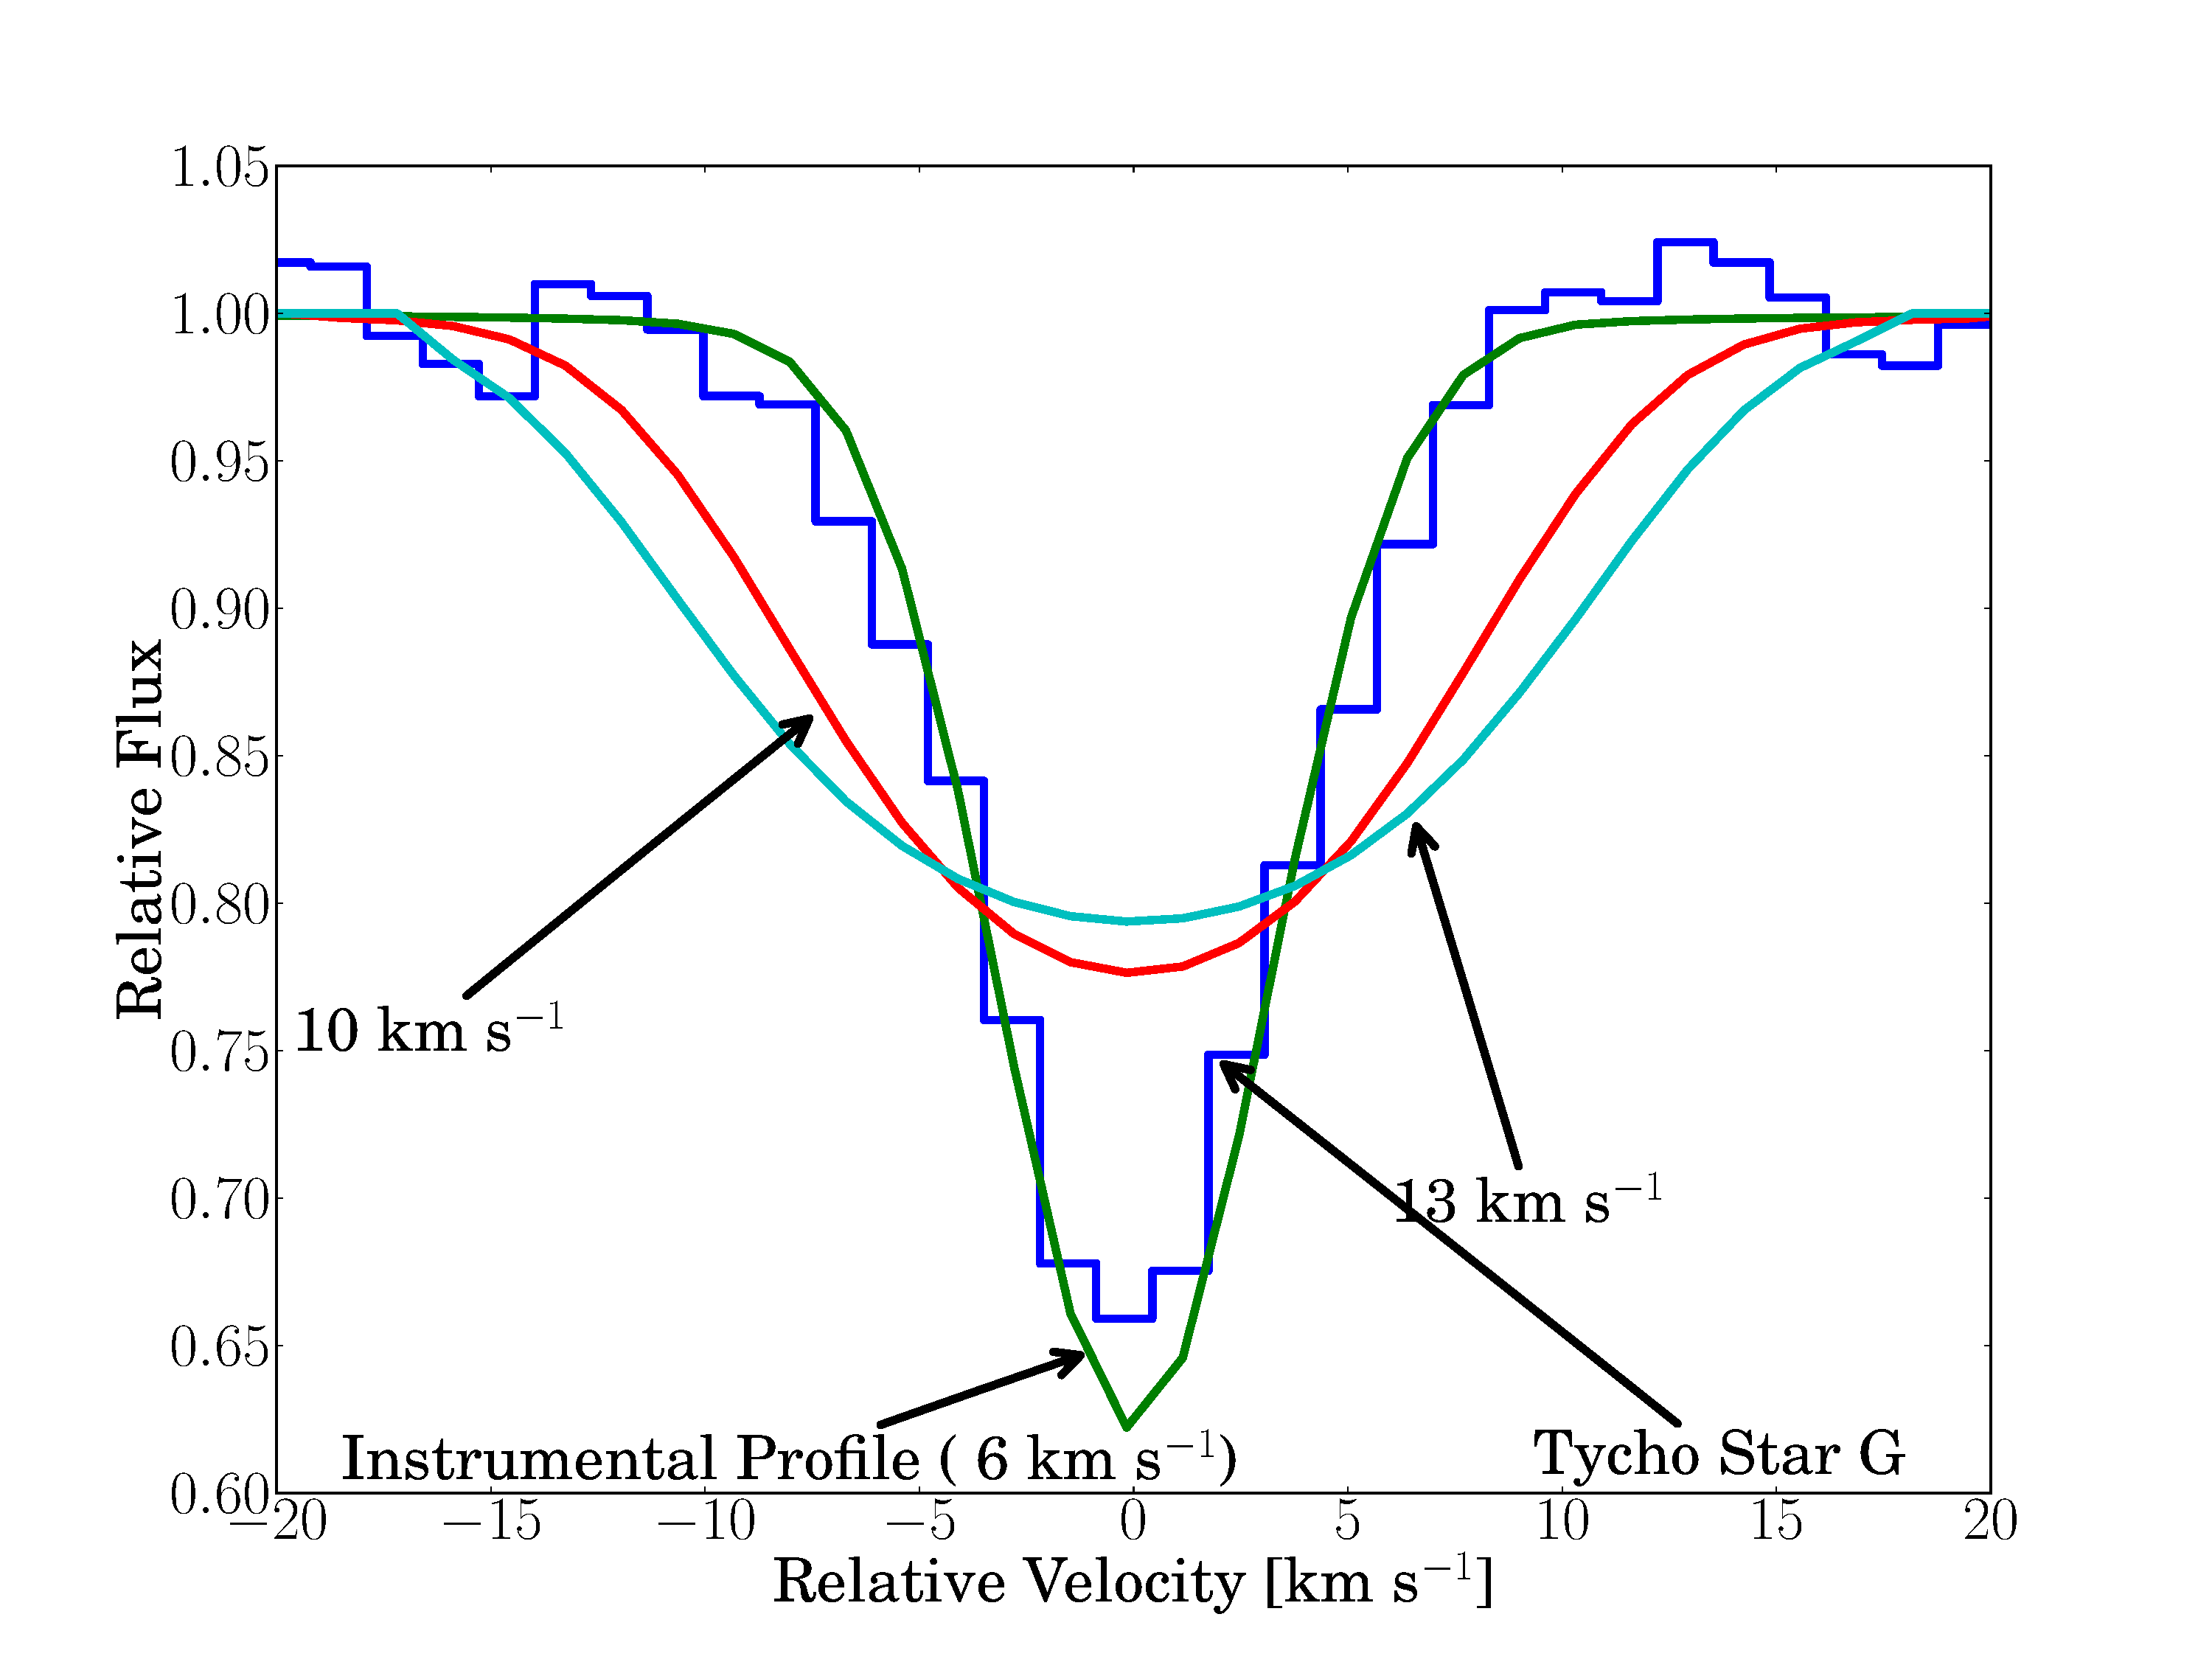
\includegraphics[width=0.45\textwidth, trim=130 30 60 0]{chapter_sn1572_hires/plots/starg_rotation.pdf} \\
\end{tabular}
\caption{The figures show the combination of Fe-line profiles after normalization to the same equivalent width and compare them to synthetic line profiles created by MOOG. We convolved the synthetic lines first with a rotational kernel with three different values for rotation and then with the instrumental profile. All stars show rotation less than 6 \kms\ which is equal to the instrumental profile at this resolution. }
\label{fig:rotvel}
\end{figure*}

Due to its high temperature and rotation, we fit the rotational velocity for \starb\ with the program \textit{sfit}\ \citep[][described in section \ref{sec:stellar-parameters}]{2001A&A...376..497J}  as part of the overall fit for this star's stellar parameters.  We find $v_{\rm rot}=171^{+16}_{-33}$\,\kms. While \starb's rotation is very high compared to the other candidate stars,  for stars of this temperature and gravity a high rotation is not unusual.


In summary, none of the stars show rotation which is measurable at this resolution.


\subsection{Stellar parameters}
\label{sec:stellar-parameters}
The stellar parameters are presented in Table \ref{table:stel_param} and were determined using a traditional spectroscopic approach based on the equivalent widths of lines of different excitation and ionization levels. . These measurements exclude \starb, due to its hot temperature, and we measure its stellar parameters by direct comparison to models, in a separate procedure.

Equivalent widths (EWs) for a set of Fe lines were measured using routines in IRAF (compiled from \citet[][henceforth Reddy03]{2003MNRAS.340..304R} and \citet[][henceforth RC02]{2002AJ....123.3277R} Table \ref{table:llist} shows the EWs measured for each of the stars. Missing values indicate that the line was not detected. 

We used the local thermodynamic equilibrium (LTE) stellar line analysis program MOOG \citemoog\ and LTE model atmospheres from the \citet{2003IAUS..210P.A20C} grid to derive an abundance for a given line. The effective temperature, \gls{teff}, was adjusted until the abundances from \ion{Fe}{1} lines displayed no trend as a function of excitation potential. The surface gravity, \gls{logg}, was adjusted until the abundances from \ion{Fe}{1} and \ion{Fe}{2} lines were in agreement. The microturbulent velocity, $\xi _{t}$ , was adjusted until there was no trend between the abundances from the \ion{Fe}{1} lines and EW. This process was iterated until self consistent stellar parameters were obtained  for each star. In our analysis, we explored stellar parameters at discrete values. For \gls{teff}, we considered values at every 25 K (e.g., 4000, 4025 K, etc.), for \gls{logg} , we considered values at every 0.05 dex (e.g., 1.00, 1.05 dex, etc.), and for $\xi _{t}$ , we considered values at every 0.05 \kms (e.g., 1.70, 1.75 \kms, etc.). We assumed that excitation equilibrium was satisfied when the slope between $\log{\epsilon}$(\ion{Fe}{1}) and lower excitation potential $(\chi)$ was $\leq0.004$. We assumed that ionization equilibrium was achieved when $\vert\log{\epsilon} ($\ion{Fe}{1}$) - \log{\epsilon} ($\ion{Fe}{2}$)\vert \leq 0.02$\,dex. The microturbulent velocity was set when the slope between $\log{\epsilon}$(\ion{Fe}{1}) and reduced equivalent width ($\log{\rm{W}}/\lambda$) was $\leq0.004$. In all cases we found appropriate solutions in which the trends between Fe I, Fe II, EW and excitation potentials were small. We estimate that the internal errors are typically $T_{\rm{eff}}\pm100$\,K, $\log{g}\pm0.3$\,dex, and $\xi _{t}\pm0.3$\,\kms. 
For further details regarding the derivation of stellar parameters, see \citet{2008ApJ...673..854Y}.

The final iron measurements are the average of \ion{Fe}{1} and \ion{Fe}{2} assuming the solar abundances of \citet{2009ARA&A..47..481A} 
In addition, we measured abundance for the Elements Ni and Li via EW analysis. We could not see any unusual abundance pattern for any of the sample stars (see Figure \ref{fig:kobayashi06}; \starb's abundances are not presented on the plot as they were measured in a different fashion).  


\ctable[
caption = {Stellar Parameters},
label = {tab:stel_param}
]
{lccccccc}{}{\FL
Name & \gls{teff} & \gls{logg} & \gls{feh} & $\Delta$\gls{feh}& [Ni/H] & $\Delta$[Ni/H] & [Li/H] \\ 
designation & (K) & (dex) & (dex) & (dex) & (dex) & (dex) & (dex) \ML 
%\startdata
\stara & 4975 & 2.9 & 0.02 & 0.16 & 0.05 & 0.025 & 0.09 \\
\starc & 4950 & 2.9 & -0.57 & 0.23 & -0.14 & -0.17 & 0.11 \\
\stare & 5825 & 3.4 & -0.16 & 0.21 & 0.2 & 0.0 & 0.131\\
\starg & 6025 & 4 & -0.15 & 0.18 & 0.14 & 0.08 & 0.11 \LL
}

\begin{figure}[h] %  figure placement: here, top, bottom, or page
   \centering
   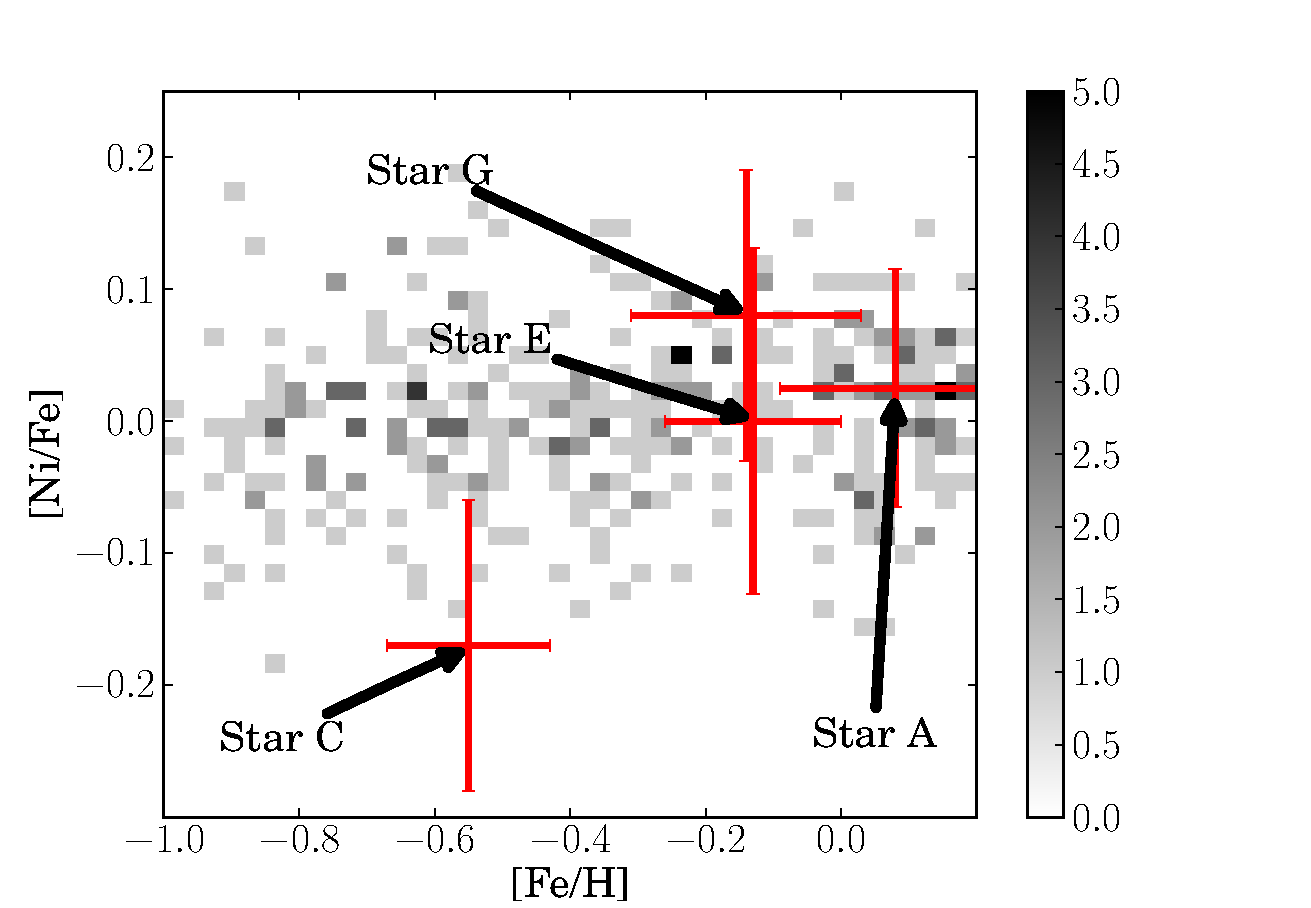
\includegraphics[width=1\textwidth]{chapter_sn1572_hires/plots/abund_chiaki.pdf} 
   \caption{The background colour indicates the distribution is taken from \citet{2006ApJ...653.1145K}. All of the measured candidates are consistent within the errors with stars of the same metallicity.}
   \label{fig:kobayashi06}
\end{figure}

In summary, the inferred metallicities for all candidates show that the candidates are of roughly solar metallicities with the exception of the metal-poor \starc. The range of metallicities spanned by the program stars is compatible with membership of the thin disk (REFERENCE). Based on metallicity alone, we do not regard any of the program stars to be unusually metal-poor or metal-rich.  Additionally, we find the [Ni/Fe] abundance to be consistent with stars of similar metallicity (see Figure \ref{fig:kobayashi06}). The stellar paramaters and elemental abundances are listed in Table \ref{tab:stel_param}.

Because Tycho B has a temperature  greater than 9000 K and is quickly rotating, the process described above cannot be used to measure stellar parameters. Instead we used the program \textit{sfit}\ \citesfit\ to match the HIRES-spectrum to a grid of model spectra. To determine the stellar parameters for \starb\ we have used a model grid with $\textnormal{[Fe/H]} = -1.0$, $8000 < T_{\textnormal{eff}} < 16000$, $7 < \log{g} < 2$. This low metallicity is suggested by a very weak Calcium K line and Mg II lines, but is hard to measure. We can not measure Helium directly in this spectrum and thus adopt N(He) = 0.1 as this is empirically a very common Helium abundance in stars.

This analysis resulted in $T_{\rm eff} = 10000^{+ 400}_{-200}\,\rm{K}$, $\log{g} = 3.67$ with slope  $\partial \log{g}/\partial T_{\rm eff} = 0.27/500 \,\rm{K}^{-1}$, rotational velocity $v\sin{i} = 171$\,\kms\ with slope $\partial v\sin{i}/\partial T_{\rm eff} = -41/500\,\rm{km\,s^{-1}\,K^{-1}}$. From qualitative analysis this object seems metal poor (e.g. in comparison to stars of similar stellar parameters but solar metallicity), but its high rotation and temperature make it hard to determine this parameter precisely. For the present, we assume [Fe/H] = -1.0 unless otherwise noted.

In addition, using the high-resolution spectrum, we measured the equivalent widths of several lines predicted to be strong in the VALD database \citep{2000BaltA...9..590K}. The abundances were deduced from the equivalent widths using a model atmosphere having $T_{\rm eff} = 10000$\,K, $\log{g}=3.67$ and [Fe/H] = -1.0 (see Table \ref{tab:starb-abund}).

One caveat regarding these abundances is the use of equivalent widths from 
single lines with large rotational broadening, since the effect of blending 
with nearby weak lines cannot be taken into account. A second is that these 
abundances invariably rely on the strongest lines, which are precisely those 
most susceptible to departures from local thermodynamic equilibrium. 
Nevertheless, they do confirm the earlier impression that the star is 
metal-poor, and justify the adoption of [Fe/H]=$-1.0 \pm 0.4$.

%ctable goes here
\ctable[
caption={\starb\ abundances},
label={tab:starb-abund},
]
{lcccccc}{}{\FL
Ion&$\lambda$& $W_{\lambda}$& $\epsilon$& $[X/H]$ & $\frac{\partial \epsilon}{\partial \log{g}}$  &$\frac{\partial \epsilon}{\partial T_{\rm eff}}$\\
designation & \AA & \AA & dex & dex& &K$^-1$ \ML
%\startdata
\ion{Mg}{2} & 4481.13+4481.33 & $220\pm15$ & $6.18\pm.08$ & -1.40&0.08&$8\times10^{-5}$ \\ 
\ion{Si}{2} & 6347.1 & $140\pm5$ & $6.96\pm.18$ & -0.59&-0.02&$1\times10^{-4}$\\
\ion{O}{1} & 7771.9+7774.2+7775.4 & $460\pm30$ & $8.43\pm.10$ & -0.58 &0.24&$-4\times10^{-5}$ \LL
}


As a second approach to determine the stellar parameters of \starb\ we used the low resolution spectra observed with LRIS.  The observation range of LRIS was chosen to be centered around the Balmer jump as this feature is sensitive to the surface gravity \citep{2007PASP..119..605B}. We fitted the spectra to a grid of model spectra \citep[]{2005A&A...442.1127M} using a spectrum fitting tool  described below. The final grid we used covered $\log{g}$ from 3.5 to 4.5 in steps of 0.5 and \gls{teff} from 9000 to 12000\,K in steps of 500\,K. In addition we expanded the grid by reddening the spectra with the \textit{pysynphot}-package\footnote{pysynphot is a product of the Space Telescope Science Institute, which is operated by AURA for NASA.}. We also added diffuse interstellar bands  \citep{1937PASP...49..224B, 1966ZA.....64..512H, 1967IAUS...31...85H, 1975ApJ...196..129H, 1995ARA&A..33...19H, 1994dib..nasa...31H, 1994A&AS..106...39J, 1958ApJ...128...57W} to the synthetic spectra , which were scaled with reddening . The included E(B-V) ranged from 0.5 to 1.3 in steps of 0.2. We assumed a rotation of 171\,\kms\ in the grid  (see section \ref{sec:rotation}).

We used $\chi^2$ as a figure of merit in our fitting procedure. To find the best fit for \starb\ we used the MIGRAD algorithm provided by \textit{MINUIT} \citep{James:1975dr} and linearly interpolated between the grid points using \textit{LinearNDInterpolator} provided by the \textit{scipy}-package  \cite{Jones:2001fk}. The fit of \starb\ results in \gls{teff}=10570\,\textrm{K}, \gls{logg}=4.05, \gls{feh}=-1.1 and E(B-V)=0.85. The model fits the synthetic spectrum poorly  in the wavelength region between 3800 -- 4280 \AA\ in (see Figure \ref{fig:starb_spec_comp}). The adopted mixing length parameter used in 1D model atmospheres used to construct the spectralgrid influences the fluxes in that region as well as affecting the hydrogen line profiles. \citet{2002A&A...392..619H} and others show that a mixing length of 0.5, rather than 1.25 as used in the Kurucz/Munari grid, better fits the violet fluxes and the hydrogen line profiles. Spectra using a mixing length parameter of 0.5 are brighter in the violet and the $\textrm{H}_\gamma$, $\textrm{H}_\delta$ and $\textrm{H}_\beta$ profiles give the same \gls{teff} as the $\textrm{H}_\alpha$ profiles. We have chosen, however, to fit the spectrum and ignore the problematic spectral region (3800 -- 4280 \AA) to avoid a systematic error. This yields \gls{teff}=10722\,K, \gls{logg}=4.13, \gls{feh}=-1.1 and E(B-V)=0.86. The differences are indicative of a systematic error in the model. We adopt the fit excluding the problematic wavelength region in the further analysis. Exploring the complex search space we estimate the error to be $\Delta\gls{teff}$=200\,K, $\Delta\gls{logg}$=0.3 and $\Delta\gls{feh}$=0.5, but acknowledge that the parameters are correlated.  



\begin{figure*}[h!]

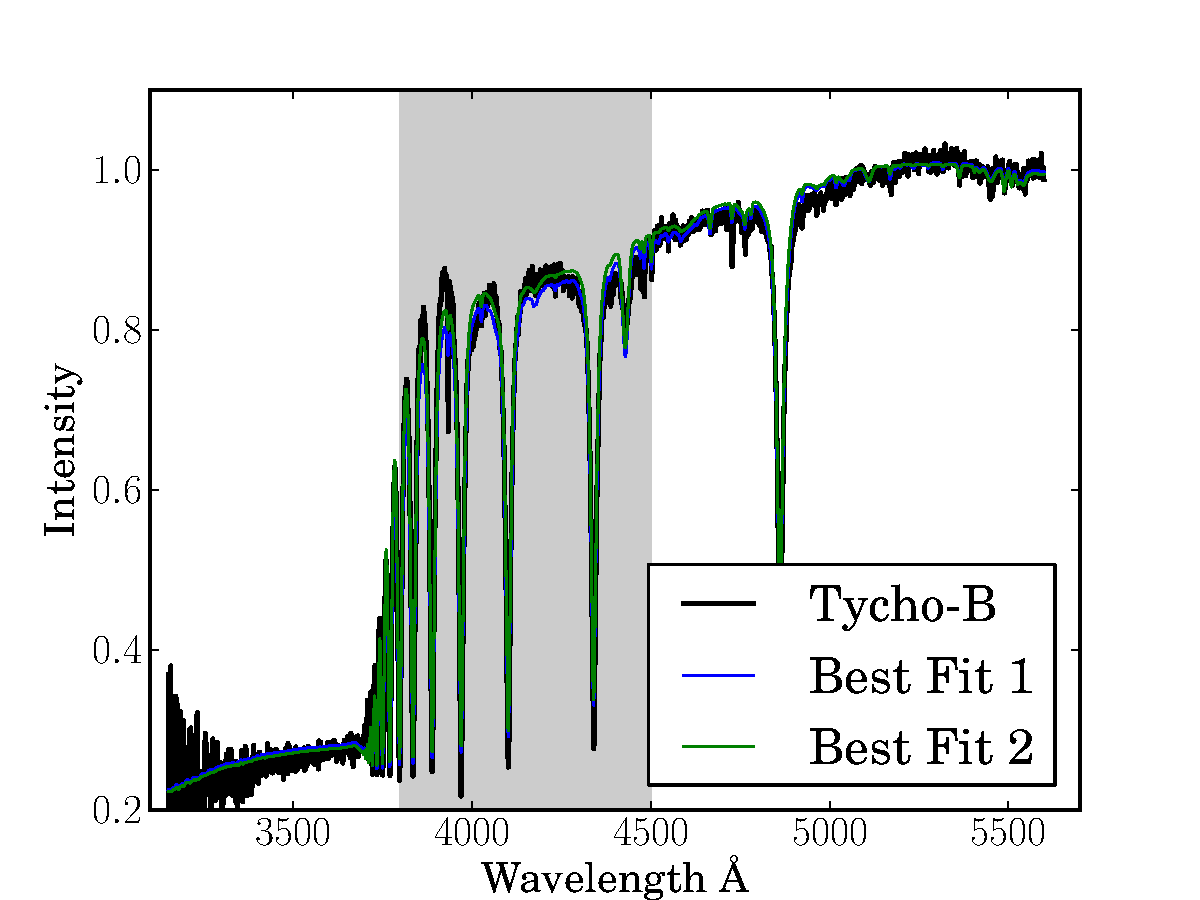
\includegraphics[width=1.\textwidth]{chapter_sn1572_hires/plots/starb_spec_comp.pdf} 

\caption{The plot shows the normalized spectrum of \starb\ with the fit which excluded the spectral region between 3800 -- 4500 \AA (Best Fit 1) and the fit with the problematic region (Best Fit 2). The region is marked with a gray shade.  }
\label{fig:starb_spec_comp}
\end{figure*}

\subsection{Distance}
\label{sec:distance}
To measure the distance to the candidate stars we used colours and absolute magnitude from isochrones by  \citet{2004ApJ...612..168P}. We used the MIGRAD algorithm  \citep{James:1975dr} to find close matches of the measured values to \gls{teff}-\gls{logg} isochrones by varying the age of the isochrone.  Subsequently we calculate E(B-V) using the isochrone's colour and we extract a mass from the isochrone. The results can be seen in Table \ref{table:iso_dist}. To estimate the errors in all distance, reddening and mass we employed the Monte-Carlo
method with 10,000 samples of \gls{teff} , \gls{logg}, \gls{feh}, B- and V-magnitude (see Figure  \ref{fig:mc_isochrone}).  Errors included in Table \ref{table:iso_dist} are the standard deviations of the Monte-Carlo sample. 
The data shows that all stars are compatible with the distance of the remnant. This is not unexpected as the uncertainties of the measurements in stellar parameters are relatively large.




\begin{figure}[htbp] %  figure placement: here, top, bottom, or page
   \includegraphics[width=0.5\textwidth]{chapter_sn1572_hires/plots/tycho-a-panel.pdf} 
   \includegraphics[width=0.5\textwidth]{chapter_sn1572_hires/plots/tycho-b-panel.pdf} 
   \includegraphics[width=0.5\textwidth]{chapter_sn1572_hires/plots/tycho-c-panel.pdf} 
   \includegraphics[width=0.5\textwidth]{chapter_sn1572_hires/plots/tycho-e-panel.pdf} 
   \includegraphics[width=0.5\textwidth]{chapter_sn1572_hires/plots/tycho-g-panel.pdf} 
   \caption{The figures show error contours for distance, extinction and mass of the candidates. The lower right shows the optimal isochrone \citep{2004ApJ...612..168P}  for the measured values of \glsentryname{teff} and \glsentryname{logg}. }
   \label{fig:mc_isochrone}
\end{figure}


\ctable[
caption = {Distances, Ages and Masses of candidate stars},
label = {table:iso_dist}
]
{lcccccc}{}{\FL
Name&Mass& $\Delta$Mass & Age & $\Delta$Age & Distance& $\Delta$Distance\\
designation& M/M$_\odot$ & M/M$_\odot$ & Gyr & Gyr & kpc & kpc \ML 
%\startdata
\stara & 2.4 & 0.8 &0.7 & 2.3 & 1.4 & 0.8\\
\starb & 1.8 & 0.4 &0.8 & 0.3 & 1.8 & 0.8\\
\starc & 0.9 & 0.4 &10.0 & 3.4 & 5.5 & 3.5\\
\stare & 1.7 & 0.4 &1.4 & 1.1 & 11.2 & 7.5\\
\starg & 1.1 & 0.2 &5.7 & 2.1 & 3.7 & 1.5\LL
}

\section{Discussion}
\label{sec:discussion}

In our sample of six stars we find no star that can be unambiguously identified as a a donor star for SN1572. On the other hand none of the stars in the sample can be completely ruled out. 

\stara\ is a metal rich giant. It seems to be likely that \stara\ is a foreground star. Its principal redeeming feature as a donor star candidate is that it is located in the geometric center of the remnant, and that it has a relatively low gravity. \stara\ shows a very low spatial motion which is consistent with a giant donor star scenario. Its lack of rotation, however, is in conflict with said scenario. 
Taking all measurements into account we regard \stara\ to be a very weak candidate.

\starb's  high temperature, position at the center of the remnant, high rotational velocity and unusual chemical abundance made it a highly unusual candidate in the Tycho Remnant center. Despite the a posteriori unlikely discovery of such a star in the remnant center, Star B's high rotational velocity coupled with its low spatial velocity, seem to be in conflict with viable donor star scenario. 
These scenarios predict that the donor star will tidally couple to the white dwarf star before explosion, causing the rotation and spatial motion to be correlated post explosion (as discussed in \wek). The large rotation seen in \starb\ should accompanied by spatial motion, which is ruled out by the observations presented here, a problem we are unable to reconcile with \starb\ being the donor star. 

 \starc\ consists of two stars which are only resolved in HST images. It consists of a brighter bluer component and a dimmer redder component (difference of ~ one magnitude in all colors) (\rl). In our analysis we find a satisfying solution for the spectrum and suspect that this is from the bluer brighter component. 
For the brighter bluer component \starc\ is a metalpoor giant, probably located beyond the remnant. \starc\ similar to \stara\ might be compatible with a giant donor star scenario. It's lack of rotation and kinematics, however, make it an uninteresting candidate.

\stard\ is roughly ten times dimmer than the close star \starc\ ($\approx 0.6$\arcsec). Our tools to measure stellar abundances are not effective for spectra with a S/N less than 10. We however compared the stars by over plotting them and determined that \stard\ is similar to \starc. Similar to \starc\ we believe \stard\ to be a very weak candidate.

\stare\ is the most distant star in this set (11.2\,kpc). It seems to be similar to  Tycho-G in temperature, however is a subgiant. It is located 7\arcsec from the geometric center and has no unusual stellar parameters or kinematics. \citet{2007PASJ...59..811I} have looked at iron absorption lines in stellar spectra made by the remnant and found \stare\ to be unusual. They suggest that a star in the background would show blue and redshifted iron lines, a star inside the remnant would only show blueshifted iron lines.  A foreground star will not show any iron features from the remnant. \citet{2007PASJ...59..811I}  suggest that \stare\ only shows blue-shifted lines and thus is suggested as being in the remnant. We believe however that \stare\ is located far behind the remnant and suggest that a low column density on the receding side of the remnant could cause a lack of red-shifted iron features.  
In summary, a lack of rotation, kinematics and distance make it a very weak candidate.

\starg\ is located 30\arcsec\ from the X-Ray center which makes it the most remote object to the center in this work. This work confirms the radial velocity measured by \gh\ and \wek. Figure \ref{fig:dist_vr} shows the exepected distribution of radial velocities from the Bescan\c{c}on model of Galactic dynamics. \starg\ is not a significant outlier at the distance of the remnant as well as behind. 
In addition, this work has analysed the proper motion of stars around the center of SN1572. Figure \ref{fig:propmot_sn1572_hires} shows \starg\ to be a slight outlier, but also shows other stars to be outliers.
The kinematic features of a donor star might easily be lost in the kinematic noise of the Galaxy. \wek, however, suggested using post-explosion stellar rotation as a possible feature for a donor star. This work suggests that \starg\ has a rotation below the instrumental profile. 
We find \starg\ to be a sub-giant star with roughly solar temperature and metallicity.
\gh\ measure a slight Ni enhancement, which they believe to originate in the contamination from the ejecta. Figure \ref{fig:kobayashi06} compares our measurement of \starg\ to the distribution of Ni and finds it to be consistent with this distribution. In addition, we could not measure a significantly enhanced Lithium-abundance as suggested in \gh. 
Finally, we have measured the distance to \starg\ and believe it to be behind the remnant. Although our error bars make it consistent with the remnant.

In summary, we acknowledge that \starg\ has unusual kinematics. However, this kinematic predicts rotation for \starg\ which we do not observe (there are caveats however, see \wek). We have not  found a satisfying explanation for \starg's large distance to the geometric center. We suggest that \starg\, has the features consistent sub-giant background interloper.

\section{Conclusion}
\label{sec:conclusion}
This work did not detect an unambiguously identifiable donor star candidate. We acknowledge that \starb\ and \starg\ have unusual features, but there has been no conclusive explanation for all their parameters. Further theoretical predictions are needed to make a more precise distinction between donors and unrelated stars. 
 
Our observations provide a case that the Tycho SNR does not have a MS, SG, or RG donor star, but other possibilities remain. These include a Helium donor, such as the so-called Sub-Chandra explosions discussed by \cite{1995ApJ...452...62L, 2010ApJ...714L..52S}. These progenitor systems might leave behind a very faint and fast moving He star. Such a progenitor would probably evade detection, and would likely not leave behind traces, such as \gls{csi} with the remnant, or early light curve anomalies \citep{2010ApJ...708.1025K}. However, deep multi-epoch wide field optical images should catch any such star speeding away from the remnant center - these are observation not yet taken.
 Finally, a double degenerate progenitor, in most cases, does not leave behind a remant , and is consistent with finding no donor star in Tycho SNR. 
 
SN 1006 and Kepler are two other \snia\ remnants in the Milky Way. SN 1006 is far from the plane and shows no signs of \gls{csi}. Kepler SNR, while far from the galaxy plane, shows \gls{csi} with its remnant, and has all the indications of what might be expected from a Single Degenerate scenario of MS or lower gravity star \citep{2011arXiv1103.5487C}. Observations of these remnant will better establish if there is a continued pattern to the unusual stars in SN Ia remnant centers, or whether the lack of viable donor stars persists in multiple systems. 
 
\section{Acknowledgments}
\label{sec:acknowledgments}
PYRAF, scipy numpy matplotlib ipython suite, kudritzki, peter wood (for fxcor),Jorge, Onken with HIRES stuff, Amanda with differential rotation


\section{Line list}
\ctable[
caption = {Measured equivalent widths from the Keck HIRES spectra},
label = {table:iso_dist},
]
{lccccccc}{}{\FL
$\lambda$ & $\chi$ & $\log{gf}$ & Source & \stara & \starg & \starc & \stare \\ 
(\AA) & (eV) & (dex) & & (dex) & (dex)& (dex) & (dex) \ML
%
%\startdata
5082.35 & 3.658 & -0.59 & Reddy03 & 6.31 & 6.44 &   & 6.2 \\
5088.54 & 3.85 & -1.04 & Reddy03 & 6.19 & 6.33 &   &   \\
5088.96 & 3.68 & -1.24 & Reddy03 & 6.21 &   &   &   \\
5094.42 & 3.83 & -1.07 & Reddy03 & 6.1 &   &   &   \\
5115.4 & 3.834 & -0.28 & Reddy03 & 6.22 &   &   &   \\
5682.20 & 4.10 & -0.47 & RC02 & 6.34 &   &   &   \\
5748.351 & 1.68 & -3.26 & RC02 & 6.33 &   & 5.74 &   \\
5749.297 & 3.94 & -1.99 & RC02 & 6.38 &   &   &   \\
5847.01 & 1.676 & -3.41 & Reddy03 & 6.26 &   & 5.55 &   \\
6007.31 & 1.68 & -3.34 & RC02 & 6.2 &   & 5.45 &   \\
6053.685 & 4.23 & -1.07 & RC02 & 6.33 &   &   &   \\
6086.28 & 4.26 & -0.52 & RC02 & 6.25 & 6.22 &   &   \\
6108.116 & 1.68 & -2.44 & RC02 & 6.26 & 6.11 & 5.33 &   \\
6111.08 & 4.088 & -0.81 & Reddy03 & 6.33 &   & 5.38 &   \\
6130.14 & 4.266 & -0.94 & Reddy03 & 6.31 &   &   &   \\
6175.37 & 4.089 & -0.55 & Reddy03 & 6.25 & 6.35 & 5.7 &   \\
6176.82 & 4.09 & -0.26 & Reddy03 & 6.3 & 6.27 & 5.43 & 6.01 \\
6177.25 & 1.83 & -3.51 & Reddy03 & 6.23 &   &   &   \\
6186.71 & 4.10 & -0.97 & RC02 & 6.33 & 6.23 &   &   \\
6204.61 & 4.09 & -1.11 & Reddy03 & 6.32 &   &   &   \\
6322.17 & 4.15 & -1.17 & RC02 & 6.31 &   &   &   \\
6370.346 & 3.54 & -1.94 & RC02 & 6.37 &   &   &   \\
6378.26 & 4.154 & -0.83 & Reddy03 & 6.3 &   & 5.81 &   \\
6482.80 & 1.93 & -2.63 & RC02 & 6.2 &   & 5.38 &   \\
6598.60 & 4.23 & -0.98 & RC02 & 6.3 &   & 5.74 &   \\
6635.12 & 4.42 & -0.83 & RC02 & 6.37 &   &   &   \\
%\tablebreak
6643.64 & 1.68 & -2.03 & Reddy03 & 6.48 & 6.02 & 5.34 & 5.97 \\
6767.772 & 1.83 & -2.17 & RC02 & 6.35 & 6.19 & 5.67 &   \\
6772.32 & 3.658 & -0.97 & Reddy03 & 6.31 &   &   &   \\
6842.037 & 3.66 & -1.47 & RC02 & 6.4 & 6.36 &   &   \\
7030.011 & 3.54 & -1.73 & RC02 & 6.42 &   &   &   \\
7122.197 & 3.54 & 0.048 & RC02 & 6.33 &   & 5.34 &   \\
7261.918 & 1.95 & -2.7 & RC02 &   & 6.26 &   &   \\
7327.648 & 3.8 & -1.77 & RC02 & 6.38 & 6.44 &   &   \\
7409.35 & 3.8 & -0.1 & RC02 &   &   & 5.24 &   \\
7414.502 & 1.99 & -2.57 & RC02 &   & 6.2 & 5.57 & 6.03 \\
7422.275 & 3.63 & -0.129 & RC02 & 6.47 &   & 5.32 & 5.84 \\
7574.048 & 3.83 & -0.58 & RC02 & 6.3 & 5.97 & 5.12 &   \\
7748.89 & 3.7 & -0.38 & Reddy03 & 6.42 & 6.17 & 5.41 & 6.27 \\
7788.93 & 1.95 & -2.42 & RC02 &   &   & 5.87 & 6.33 \\
7797.59 & 3.9 & -0.35 & Reddy03 & 6.41 & 6.16 & 5.59 & 6.2 \\
7917.44 & 3.74 & -1.5 & RC02 &   & 6.14 &   &   \LL
}




% !TEX root = ../thesis.tex
\chapter{Progenitor search in SN 1006}
\label{chap:sn1006}


\section{Introduction}

The search for a donor star in \sn{1572}{}\ has not turned up an obvious candidate. However, we have detected two objects (\starb\ and \starg) exhibiting some unusual properties, which while interesting, ultimately seem inconsistent with the expectations of any viable donor star scenario. \Gls{donor} star scenarios are theoretical in their nature and any actual donor star is likely to not exhibit all features predicted by the model. Therefore, we have reached an impasse with \sn{1572}{} and more detailed observations will likely not provide a definitive answer if either of these two stars were involved in the progenitor system. An obvious way forward is to scrutinise stars in other \snia\ remnants and see if any of those have similar properties to \starb\ or \starg. The remnant of \sn{1006}{} is the ideal object for this kind of follow-up search. 

The lack of a central neutron star, observation of several tenths of a solar mass of iron inside the remnant \citep{1997ApJ...481..838H} and the the high peak luminosity and basic light curve shape \citep[visible for several years][]{1965AJ.....70..748G} all indicate that \sn{1006}{} was a \snia. The remnant has a secure distance, measured by \citet{2003ApJ...585..324W}, who combined the proper motion and the radial velocity of the expanding shell to measure the distance to 2.2~\kpc, making \sn{1006}{} the closest of the ancient \snia\ remnants (consistent \sn{1006}{} being the brightest).   The geometric centre of the remnant is well determined from both \xray\ and radio observations \citep{2003ApJ...585..324W}. In addition, the interior of the remnant has been probed with UV background sources \citep{2005ApJ...624..189W}. 

This revealed the aforementioned iron core as well as a silicon-rich shell. The remnant has been searched for possible objects associated with the supernova explosion previously, and an unusual O-star had been identified as a possible donor star to \sn{1006}{}. This unusual O-Star was identified near the centre of \sn{1006}{} by \citet{1980ApJ...241.1039S} and is now called Schweizer-Middleditch Star (\smstar). After successful identifications of neutron stars in both the Vela Remnant and the Crab Remnant this was thought to be the third identification of a stellar remnant in a historical supernova. Subsequent UV spectroscopic follow-up of the \smstar\ by \citet{1983ApJ...269L...5W}, showed strong \ion{Fe}{2} lines with a profile broadened by a few thousand \kms. In addition, \citet{1983ApJ...269L...5W} identified redshifted \ion{Si}{2}, \ion{Si}{3} and \ion{Si}{4} lines. Their conclusion was that these absorption lines stem from the remnant and place the \smstar\ behind the remnant, making it unrelated to \sn{1006}{}. Although unrelated, the \smstar\ is an ideal object to probe the remnant and measure upper limits for interstellar extinction \citep[E(B-V) = 0.1][]{1993ApJ...416..247W,2003ApJ...585..324W}.


SN 1006 has several properties which make it well suited to undertake a progenitor search.  Although the remnant is the oldest among the known \snia\ remnants, its age is still young enough that  the remnant's centre is well determined, and the motion of any potential donor star low enough that only a small area of stars need to be searched. Furthermore, this elapse of 1005 years is a short length of time relative to the timescales of stellar evolution for donor stars \cite[see][]{2000ApJS..128..615M} - we still expect a potential donor star to be close to the same state as directly after the supernova explosion. In addition, \sn{1006}{} has a low interstellar extinction, which eases the determination of stellar parameters. These serendipitous conditions for the \sn{1006}{} remnant led us to launch a photometric and spectroscopic campaign to search for the donor star. Our photometric observations were taken at Siding Spring Observatory with the 2.3m Telescope imager. The spectroscopic observations were undertaken with the high resolution multi-object spectrograph \gls{flames} attached to the \gls{vlt}.


In Section \ref{sec:obs_red} we outline the observations as well as data reduction of the photometric and spectroscopic data. Section \ref{sec:sn1006_analysis} is split into four subsections, namely radial velocity, stellar rotation and stellar parameters. We conclude this chapter in Section \ref{sec:sn1006:conclusion} and discuss the possible implications of our initial find as well as outlining some future work.


\section{Observations and Data Reduction}
\label{sec:obs_red}
\subsection{Photometric Observations}
\Gls{ccd} images of \sn{1006}{} were obtained using the imaging camera at the Nasmyth-B focus of the ANU 2.3~m Telescope at
the Siding Spring Observatory, on 11 May 2004. We exposed for 1860~s in U-Band, 1490~s in B-Band, 788~s in V-Band and 1860~s in I-Band. For calibration purposes we took images of the PG1633 and PG1047 standard star regions in the same filters. The seeing ranged between 1\arcsec and 2\arcsec, and the conditions were photometric. 
The data were bias corrected and flatfielded (using skyflats) using \gls{pyraf}.

For our photometric data reduction we fitted an astrometric solution using astrometry from the \twomass\ point source catalogue \citep{2006AJ....131.1163S} to our frames. 
We used \gls{sextractor} to measure the magnitudes of the objects in the frames and then calibrated our photometry to a standard Bessell Filter system using the Stetson magnitudes \footnote{This research used the facilities of the Canadian Astronomy Data Centre operated by the National Research Council of Canada with the support of the Canadian Space Agency} of our standard fields PG1633 and PG1047 .  

The measured magnitudes were supplemented with near infrared magnitudes from the \twomass\ point source catalogue (see Table \ref{tab:sn1006_twomass} and \ref{tab:sn1006_photometry} ). Subsequently we checked the photometric measurements, by plotting the obtained $B-V$ colours against the $V-K$ colours (see Figure \ref{fig:colour_check}).
\begin{figure}[htbp] %  figure placement: here, top, bottom, or page
   \centering
   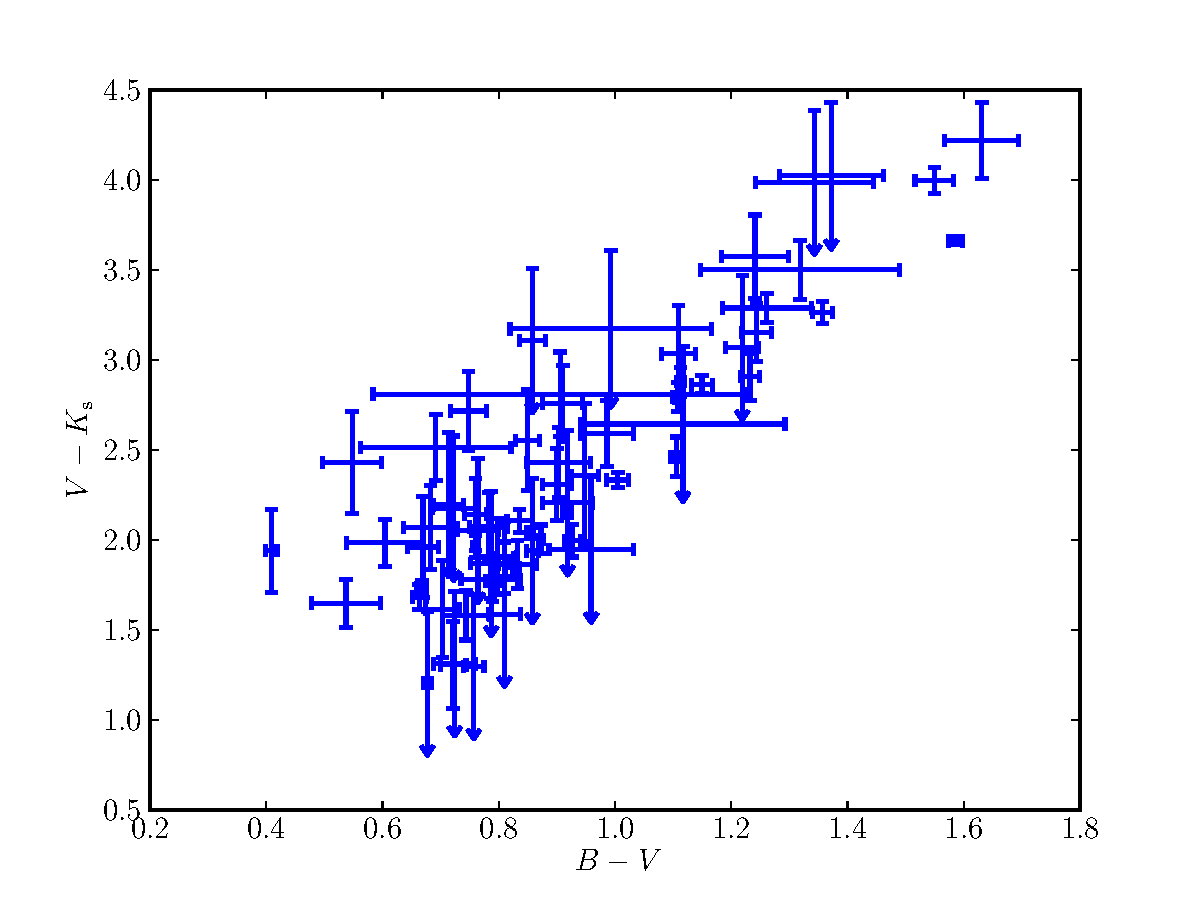
\includegraphics[width=\textwidth]{chapter_sn1006/plots/color_bv_vk.pdf} 
   \caption[Colour-colour plot of all candidates in SN 1006 to check photometry]{Colour-colour plot of all candidates in SN 1006 to check photometry. The correspondence is as expected given the uncertainties in the measurements.}
   \label{fig:colour_check}
\end{figure}

We have also computed temperatures from photometric colours by using the polynomials given in \citet{2010A&A...512A..54C}. In the first instance, we assumed a solar \gls{feh} for all stars, but the choice of \gls{feh} only has a minor influence on the temperature calculation (e.g. change of 300K between \feh=0 and \feh=-1) for the temperature. In addition, the temperature polynomial coefficients incorporating the metallicity are particularly small for the $V-K$ colour. All temperatures are listed in the optical photometry Table \ref{tab:sn1006_photometry} and infrared photometry Table \ref{tab:sn1006_twomass}.


\subsection{Spectroscopic Observations}

For the spectroscopy survey we used the \gls{vlt} instrument \gls{flames}, which can provide high resolution (R=25,000) optical spectra over a 25\arcmin\ field of view for up to 130 objects. In this mode, the spectral coverage is limited to 200~\AA, and we chose the wavelength region from 5139~\AA\ to 5356~\AA\ which contains the gravity sensitive \gls{mgb} Triplet as well as many iron lines to accurately measure metallicity. For the centre of our spectroscopic survey we chose the mean of the \xray\ and radio centre \citep[\rasc{15}{02}{22}{1}\ \decl{-42}{05}{49};][]{2003ApJ...585..324W}. We chose a search radius of 120\arcsec\ - corresponding to the motion of a star travelling 1250~\kms at 2.2~\kpc\ over 1000 years. This generous choice, which is more than four times our maximum expected escape velocity (see Figure \vref{fig:han2008_vrad}), was made to accommodate any errors in the choice of the centre. Although the models predict the surviving companion to be several hundred \lsun\ \citep{2000ApJS..128..615M}, we chose a limiting magnitude of $V=17.5$ ($0.5~\lsun(V)$ at 2.2~\kpc\ including extinction of E(B-V)=0.1) to accommodate a wide range of potential \gls{donor} stars. An exposure time of 3.8~hours was chosen to obtain spectra with high enough quality to measure rotation and basic stellar parameters (\snratio\ $>20$). For completeness and to not waste fibres we chose additional stars down to a magnitude limit of $V=19$, which are only used for radial velocity measurements. These constraints yielded 26 stars with $V<17.5~\textrm{mag}$ and 53 stars in the bin between $17.5<V<19~\textrm{mag}$ (for a total of 79 stars) for our survey (see Figure \ref{fig:overview_sn1006}). With fibre buttons not being able to be placed less than 11\arcsec\ apart, we had to split our candidates over three different setups. The first two setups were observed five times with 2775~seconds each. We deliberately chose bright stars for the last setup so that it only had to be observed three times with 2775 s each. In addition, we placed spare fibres on three bright stars (R$\approx 10$; 2MASS J15032744-4204463, 2MASS J15031746-4204165, 2MASS J15033195-4202356) located close to the edge of the 25\arcmin\ field of view for calibration purposes. Additional spare fibres were placed on sky positions, which were chosen to be far from \twomass\ sources and manually inspected on DSS images to be in star free regions.
\begin{figure}[tb] %  figure placement: here, top, bottom, or page
   \centering
   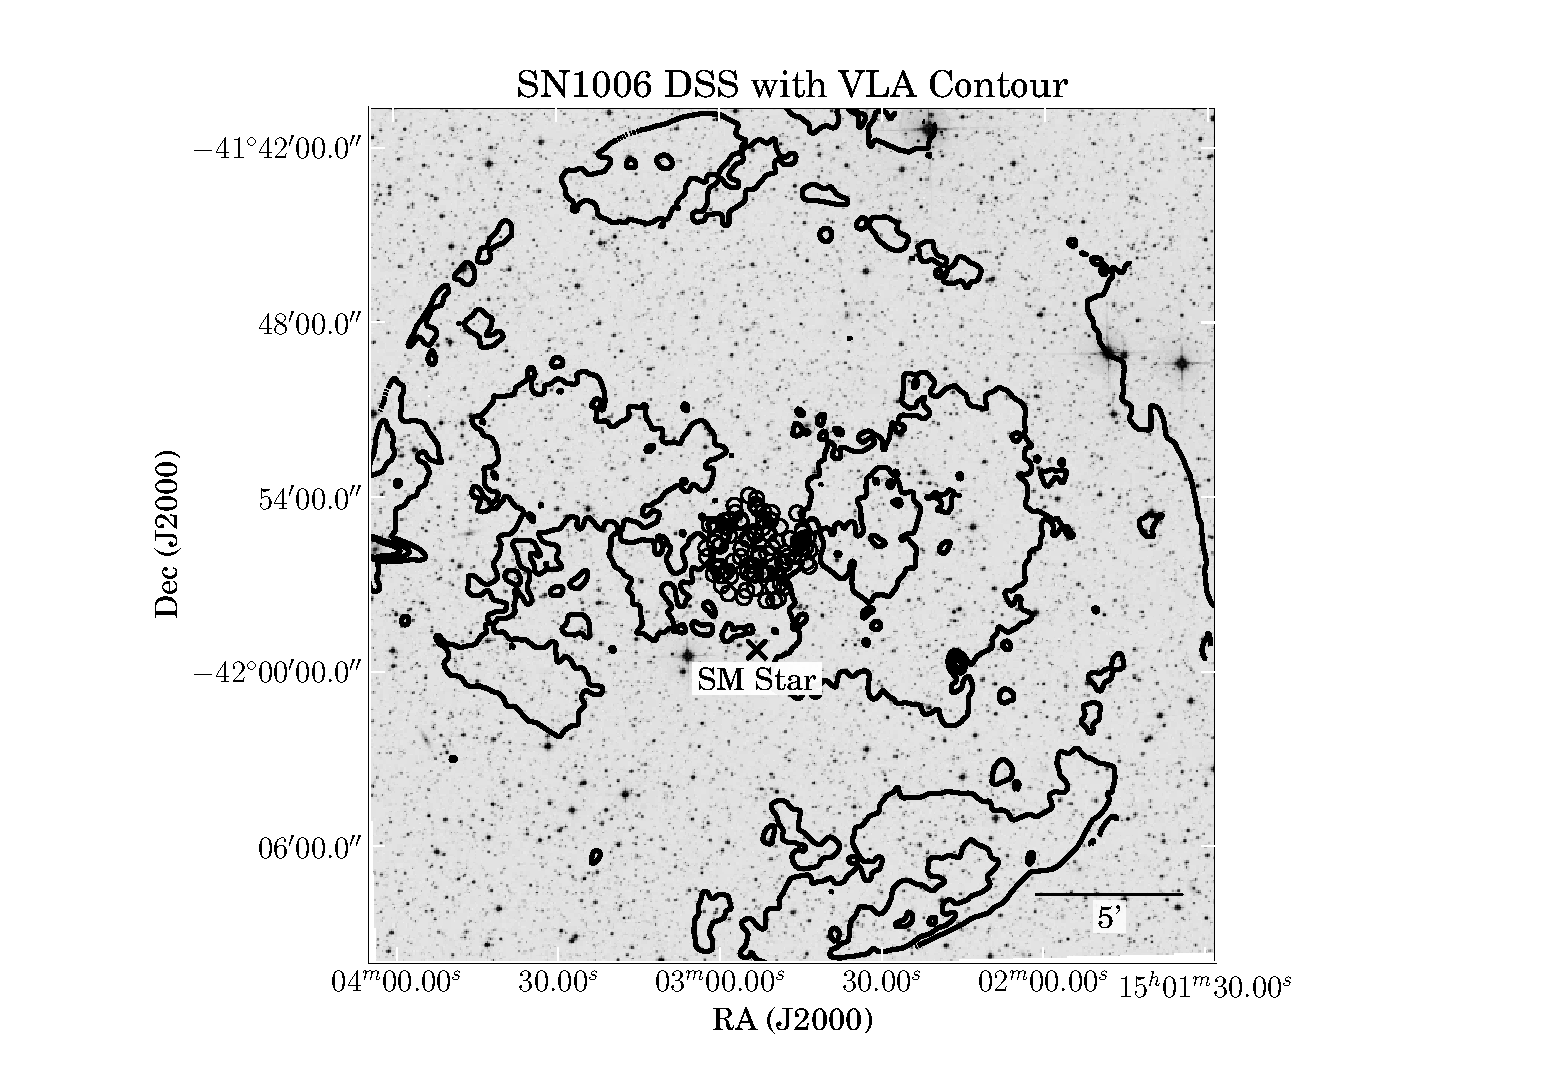
\includegraphics[width=\textwidth, trim=2cm 0 4cm 0, clip]{chapter_sn1006/plots/sn1006_overlay_withsm.pdf} 
   \caption[Overview of candidates and remnantin SN 1006]{Optical DSS image with radio contour overlay (VLA). The black circles in the centre show the 79 program stars. Additionally we have marked the `spurious` donor the \smstar.}
   \label{fig:overview_sn1006}
\end{figure}
In addition, to our night time calibration, which included simultaneous arc exposures with four fibres for each observation block, we received standard daytime calibrations. In total, 13 observation blocks with an exposure time of 2775~seconds each were obtained. Table \ref{tab:observations} provides the Observing ID, modified julian date, mean seeing, mean airmass, setup name and heliocentric correction for all observations (all data is available under ESO Program ID: 083.D-0805(A)). Due to broken fibres, not all stars where observed for the expected length of time. Broken fibres caused \candstar{31} not to be observed at all in this project (see Figure \ref{fig:sn1006:zoomed_overview}) - although a $V=17.87~\textrm{mag}$ is not part of our primary sample.
\begin{deluxetable}{cccccc}
\tablecaption{Observations}
\tablehead{\colhead{ObsID} & \colhead{MJD} & \colhead{FWHM} & \colhead{Airmass} & \colhead{SetupName} & \colhead{$\Delta v_{\rm helio}$}\\ 
\colhead{-} & \colhead{d} & \colhead{\arcsec} & \colhead{-} & \colhead{-} & \colhead{\kms}}


\startdata
360737 & 54965.1 & 1.2 & 1.2 & SN1006 1 & 1.5\\
360739 & 54965.1 & 1.2 & 1.1 & SN1006 1 & 1.5\\
360740 & 54965.1 & 1.0 & 1.1 & SN1006 1 & 1.4\\
360741 & 54985.0 & 0.7 & 1.4 & SN1006 1 & -7.4\\
360742 & 54964.2 & 1.5 & 1.1 & SN1006 1 & 1.7\\
360743 & 54985.0 & 0.8 & 1.2 & SN1006 2 & -7.5\\
360745 & 54985.0 & 0.9 & 1.1 & SN1006 2 & -7.6\\
360746 & 54985.1 & 1.0 & 1.1 & SN1006 2 & -7.7\\
360747 & 54985.1 & 1.0 & 1.1 & SN1006 2 & -7.7\\
360748 & 54985.2 & 0.9 & 1.1 & SN1006 2 & -7.8\\
360749 & 54963.1 & 1.2 & 1.2 & SN1006 3 & 2.4\\
360751 & 54963.1 & 1.1 & 1.1 & SN1006 3 & 2.3\\
360752 & 54963.2 & 1.1 & 1.1 & SN1006 3 & 2.3\\
\enddata
\label{tab:observations}
\end{deluxetable}


\begin{figure}[tb] %  figure placement: here, top, bottom, or page
   \centering
   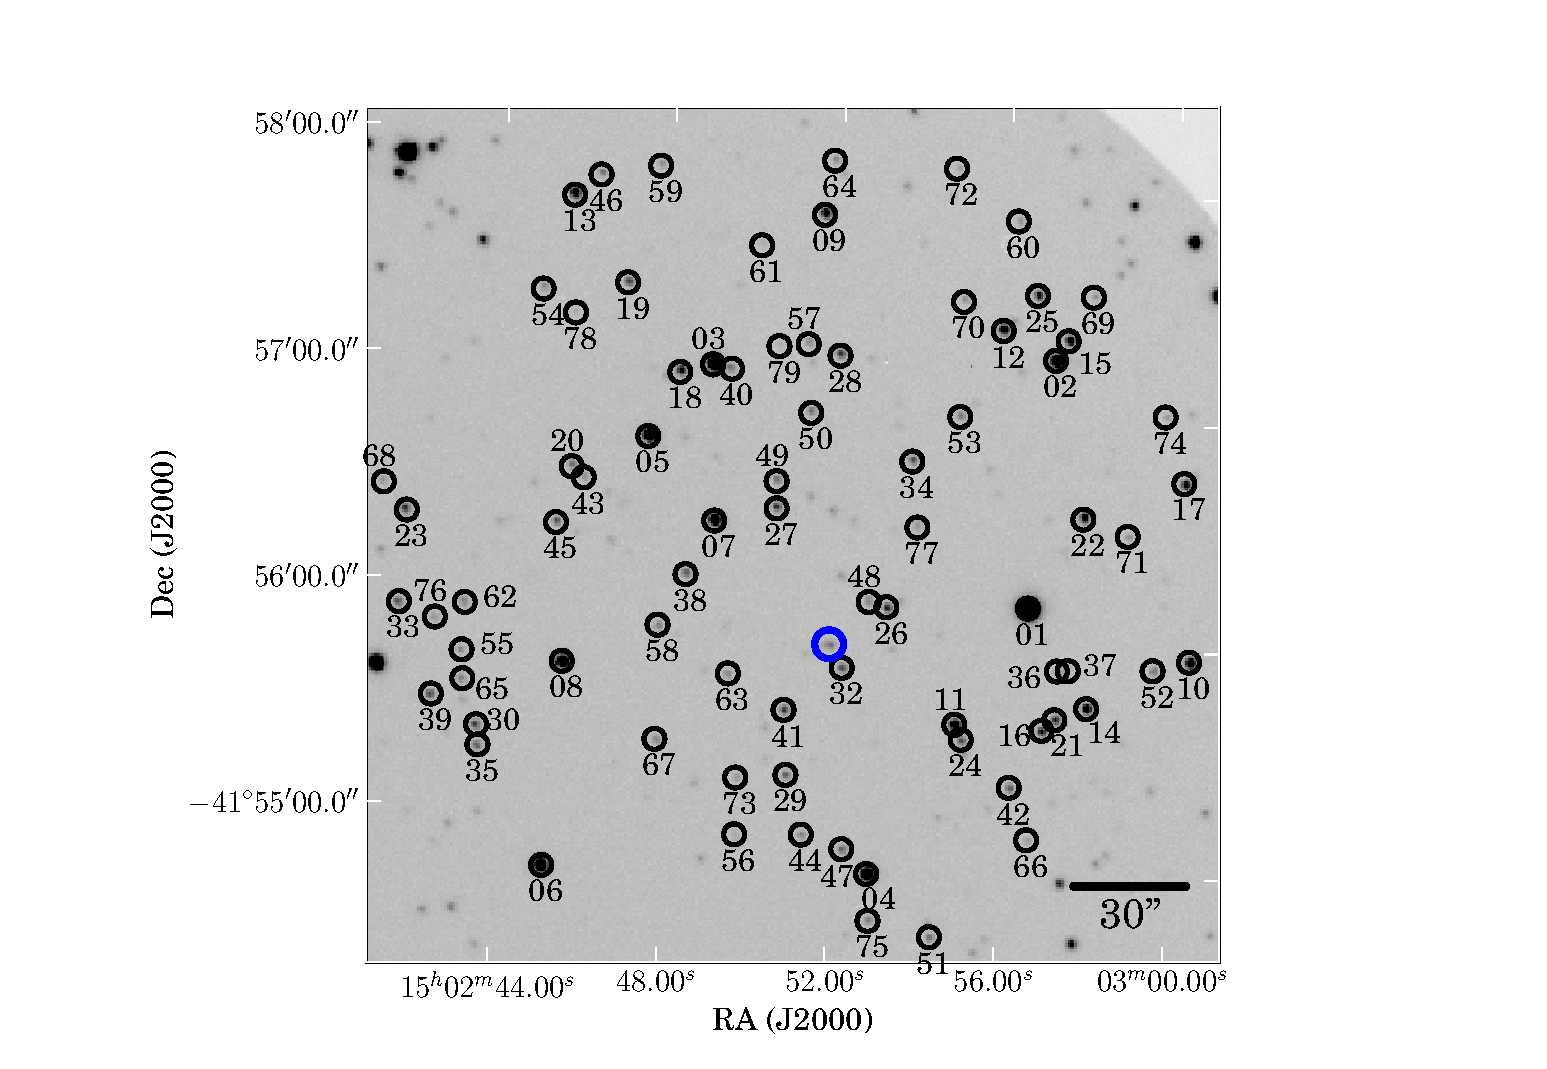
\includegraphics[width=\textwidth, trim=2cm 0 5cm 0, clip]{chapter_sn1006/plots/overview_labeled_sn1006.pdf} 
   \caption[Close-up of the candidates in SN 1006] {V-Band image taken by the 2.3~m Telescope. We have marked \candstar{31}, which was not observed due to broken fibres, with a blue circle. With the a brightness of $V=17.87$ \candstar{31} is fainter than our primary catalog ($V<17.5$~mag), and is the only star which lacks a spectrum to $V=19~\textrm{mag}$ in the remnant's centre.}
   \label{fig:sn1006:zoomed_overview}
\end{figure}


We first applied a cosmic ray removal tool on the raw 2D frames \citep{2001PASP..113.1420V}. The data was then reduced with the ESO-CPL pipeline (version 5.2.0), using the GIRAFFE instrument recipes (version 2.8.9). The only variation that was made to the default parameters was the usage of the Horne extraction algorithm instead of the "Optimal"-extraction algorithm. This yielded 366 individual spectra of the candidate stars and an additional 39 calibration star spectra. 


\section{Analysis}
\label{sec:sn1006_analysis}
\subsection{Radial Velocity}

\begin{figure}[tb] %  figure placement: here, top, bottom, or page
   \centering
   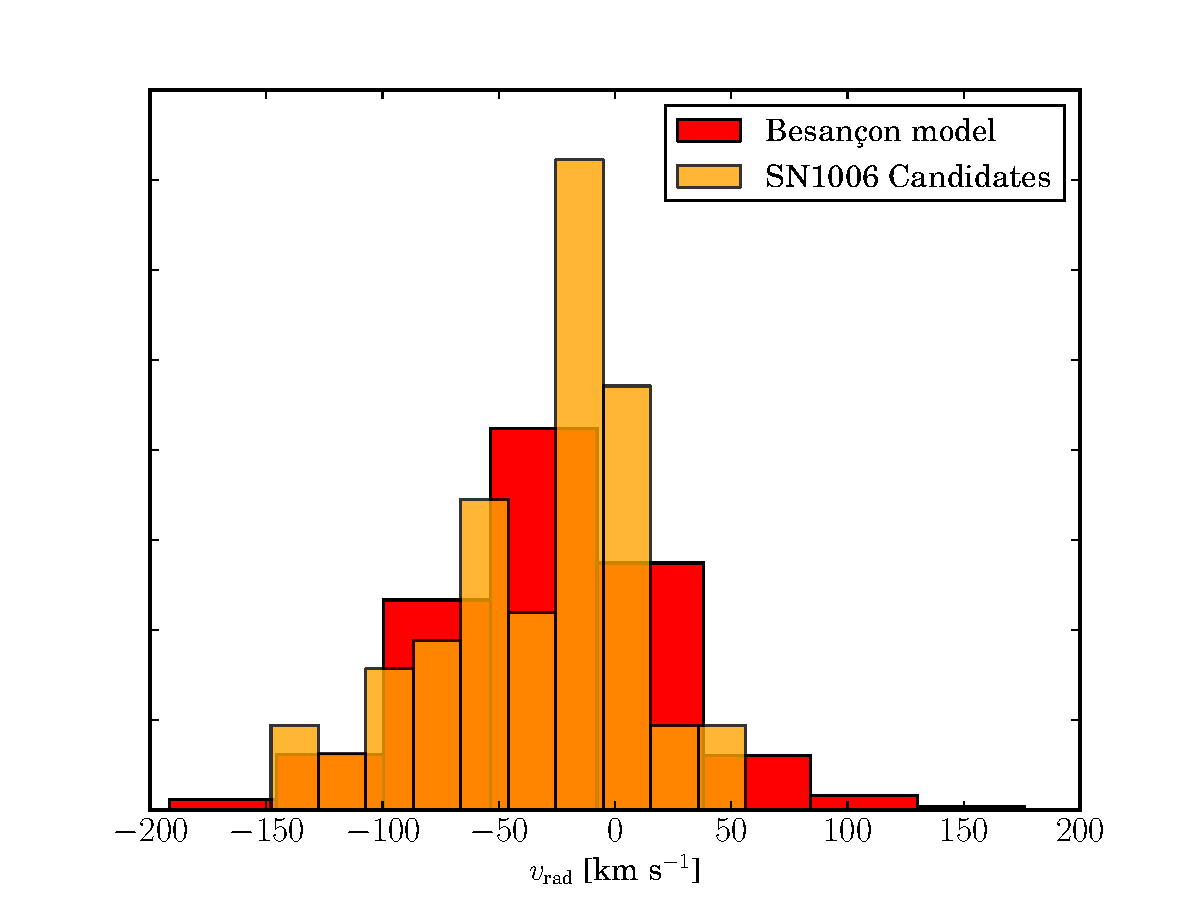
\includegraphics[width=\textwidth]{chapter_sn1006/plots/sn1006_vrad_besancon.pdf} 
   \caption[Radial velocity of all candidates in SN 1006 compared with Besan\c{c}on Model]{Comparison of all candidate stars with the distribution of stars taken from the the Besan\c{c}on kinematic model. The model input parameters were a search area of 1 square degree around the centre of \sn{1006}{} and a magnitude limit of $10<\textrm{V}<17.5$}
   \label{fig:sn1006_vrad_comp}
\end{figure}


To obtain radial velocities we employ a two step process. We used a solar spectrum from \citet{1984sfat.book.....K} with the standard cross-correlation technique described in \citet{1979AJ.....84.1511T} and implemented in the \gls{pyraf} task \textsc{fxcor}. The cross-correlation was performed on each individual spectrum. The results were then heliocentrically corrected, and then averaged for each star with a sigma clipping algorithm (see Table \ref{tab:sn1006_kinem}). We note that especially for faint objects we observe a second cross-correlation peak at 0~\kms and believe that this is reflected sun light from the moon. We believe that this has a negligible effect on our radial velocity measurement.
In Figure \ref{fig:sn1006_vrad_comp} we have compared our radial velocity measurements with the Besan\c{c}on kinematic model of the Milky way \citep{2003A&A...409..523R}. Our selection criteria for creating the  Besan\c{c}on kinematic model was all stars within 1 square degree of \sn{1006}{} and a magnitude cut of $10<\textrm{V}<17.5$. We compared the resulting 10000 stars to our 78 stars in the sample in Figure \ref{fig:sn1006_vrad_comp}. 




\subsection{Rotational Velocity}
\label{sec:sn1006_rotvel}
Due to the direction looked through the Galaxy, there is a large velocity spread in the direction of \sn{1006}{} (see Figure \ref{fig:sn1006_vrad_comp}) making it hard to isolate a \gls{donor} star based just on kinematic features. A distinguishing feature for a \gls{donor} star should be rotation (discussed in Chapter \ref{chap:sn1572_starg}), especially if the donor star isn't a giant. The rotational velocities in Chapters \ref{chap:sn1572_starg} \& \ref{chap:sn1572_hires} were all measured manually. In these previous measurements we selected weak iron lines and stacked them to obtain a line profile, which was compared to synthetically rotationally broadened lines. This was a feasible way for six spectra, it is however not feasible for more than 200 spectra. 

Measuring repetitive structures like line profiles is much more straight forward in Fourier space. The intrinsic spectrum ($f_\textrm{spectrum}$) of a star is broadened by a convolution of the intrinsic spectrum with a rotational broadening kernel ($g_\textrm{rotation}$). The next broadening is introduced by the instrument (instrumental kernel $h_\textrm{instrument}$) before being recorded on the detector. Assuming an unbroadened synthetic spectrum ($f_\textrm{synthetic}$), matching the intrinsic stellar spectrum, we can describe a convolution in Fourier space as,
\begin{align*}
	f_\textrm{observed} =& f_\textrm{spectrum} \otimes \underbrace{g_\textrm{rotation} \otimes h_\textrm{instrument}}_{f_\textrm{profile}}\\
     F(f_\textrm{spectrum} \otimes g_\textrm{rotation} \otimes h_\textrm{instrument}) =& F(f_\textrm{spectrum}) \times F(g_\textrm{rotation}) \times F(h_\textrm{instrument})\\
     \Rightarrow \frac{F(f_\textrm{observed})}{F(f_\textrm{synthetic})} \approx& F(f_\textrm{profile}),
\end{align*}
where $F$ denotes the Fourier transform. This yields the line profile which we can separate, knowing the resolution of the instrument, into an instrumental profile and a rotational kernel . This technique has been described by a selection of authors \citep[e.g.][]{1977ApJ...211..198G}. \textsc{fxcor} uses this technique to measure radial velocities from shift of the profile peak relative to rest. We have applied this technique successfully to extract the rotation for some of the stars were the quality of the spectra was adequate (see Table \ref{tab:sn1006_kinem}).


\subsection{Stellar Parameters}
\label{sec:sn1006_stelparam}

We obtained detailed stellar parameters for the donor candidates with $V<17.5$ by employing a grid based technique (three dimensional grid in \teff, \logg\ and \feh). \gls{moog} was used to synthesise the spectral grid using the model stellar atmospheres by \citet{2003IAUS..210P.A20C}. Line wings were taken into account up to 8~\AA\ away from line centre, which seemed to be a reasonable compromise between grid creation time and accuracy. For the atomic lines we merged values from the \gls{vald} with adjusted values (to reproduce the Arcturus and the Sun) from \cite{2008A&A...486..951G}. In addition, we used the measured molecular lines described in  \citet{1995KurCD..23.....K}. The final grid extends from 3500~K to 7500~K in \gls{teff} with a step size of 250~K, in \gls{logg} it ranges from  0 to 5 with a stepsize of 0.5 and in \feh\ it ranges from -2.5 to 0.5 with a stepsize of 0.5 (with an extra set of points at 0.2). 

We used the appropriate sections from the Solar spectrum \citep{1984sfat.book.....K} and the Arcturus spectrum \citep{2000vnia.book.....H} to calibrate our spectral grid. We measured stellar parameters by first finding the best fitting grid point and then using the minimizer \gls{minuit} to find a minimum by interpolating between the gridpoints \citep[described in Appendix \ref{chap:ndinterp} of this thesis;][]{Barber96thequickhull}. For the Sun we obtain stellar parameters of \teff=5825~K, \logg=4.4 and \feh=-0.12 and for Arcturus we obtain stellar parameters of \teff=4336~K, \logg=1.9, \feh=-0.67. We acknowledge the error in measurement, but believe our spectral grid to be accurate enough for distinguishing a potential donor candidate against an unrelated star. 

To measure our observed spectra we first fitted the continuum with Legendre polynomials with a maximum order of 3 and a sigma clipping algorithm discarding the lines. The order that gave the lowest \gls{rms} of the fit was used. We then combined the spectra using the previously measured \gls{vrad} and the computed heliocentric correction. In addition, we broadened the synthetic spectral grid with a rotational kernel for each star where applicable. These spectra were then fitedt using the previously described algorithm, except that we added the $B-V$ photometric temperature as a prior. As the photometric temperature uses the metallicity as an input parameter we recalculated the photometric temperature prior using the metallicity determined by the fit. This procedure was repeated until the gravity estimate converged to less than 0.1~dex. We believe our temperatures to be good to a few hundred K, our surface gravities as well as metallicities have a systematic uncertainty of roughly 0.5~dex. 

The stellar parameters can be seen, as fits to the spectra, in Figure \ref{fig:sn1006_candfit} and in tabulated form in Table \ref{tab:sn1006_stel_param}. The final set of stellar parameters shows a typical distribution of many dwarfs and a few giants. None of the stars seem to be unusual in any way. Giant stars, which are expected to have relatively low \vrot\ post explosion (but still $> 20~\kms$), are absent from the remnant's centre. 
%!TEX root = ../../thesis.tex
\ctable[
caption=SN 1006 candidates ($V<17.5$) stellar parameters,
label={tab:sn1006_stel_param},
width=\textwidth
]
{lXXXXX}{}{\FL
Name & $\teff $ & $\logg$ & \feh & 
V&\vrot \\ 
 & K & dex & dex& mag&\kms \ML
01 & 4285 & 2.0 & $-1.0$& $13.50$ &$<10$\\
02 & 4001 & 0.8 & $-1.4$& $15.37$&$<10$\\
03 & 5446 & 4.0 & $-0.6$& $15.04$&$<10$\\
04 & 5347 & 4.0 & $-0.6$& $15.47$&$<10$\\
05 & 5191 & 3.7 & $-0.6$& $15.50$&$<10$\\
06 & 5874 & 4.5 & $-0.7$& $15.50$&$<10$\\
07 & 4884 & 4.2 & $-0.8$& $15.90$&$<10$\\
08 & 5954 & 4.2 & $-0.5$& $15.86$&$<10$\\
09 & 4217 & 3.9 & $-2.5$& $16.58$&$<10$\\
10 & 5662 & 4.3 & $-0.8$& $16.30$&$10$\\
11 & 5489 & 4.1 & $-0.8$& $16.33$&$<10$\\
12 & 5313 & 4.4 & $-0.9$& $16.39$&$16$\\
13 & 5114 & 4.0 & $-0.7$& $16.49$&$<10$\\
14 & 5245 & 4.3 & $-0.7$& $16.56$&$<10$\\
15 & 5503 & 4.2 & $-0.7$& $16.63$&$<10$\\
16 & 4448 & 4.0 & $-1.8$& $17.26$&$14$\\
17 & 5515 & 4.4 & $-1.2$& $16.66$&$<10$\\
18 & 5341 & 4.1 & $-0.9$& $16.77$&$12$\\
19 & 3846 & 4.1 & $-2.4$& $17.39$&$17$\\
21 & 4510 & 3.1 & $-1.3$& $17.36$&$13$\\
22 & 6448 & 4.2 & $-0.4$& $16.71$&$13$\\
23 & 4429 & 4.0 & $-1.8$& $17.39$&$14$\\
25 & 6119 & 4.9 & $-0.7$& $17.03$&$<10$\\
26 & 5619 & 4.0 & $-1.1$& $17.23$&$<10$\\
27 & 5336 & 4.0 & $-1.3$& $17.47$&$<10$\\
28 & 5379 & 4.3 & $-1.1$& $17.43$&$<10$\\
\LL}


\section{Conclusions}
\label{sec:sn1006:conclusion}
In this work we have scrutinised all stars to a limit of $0.5~\lsun(V)$ at the distance of the \sn{1006}{}\ remnant. None of the stars scrutinised in our sample show features consistent with those expect for donor star models. 

Giant star progenitors are easily ruled out because there is no star bright enough to be at the distance of the remnant. \citet{2000ApJS..128..615M} suggests that giant donors have a luminosity of $\approx 1000~\lsun$ ($V\approx9$ at the distance of the remnant) for at least 100,000 years. Furthermore, these models suggest that the giant donor is likely to have a high temperature of more than $10^4\,K$. In addition, the star should have some rotation in excess of what has been measured for any of the stars in this sample. In summary, there is no viable giant star donor star scenario for the stars located in \sn{1006}{}. 

Sub giant donors should also be very luminous \citep{2000ApJS..128..615M} with a minimum expected luminosity of $L\approx500\,\lsun$ ($V\approx9.7$ at the distance of the remnant) lasting for 1400--11,000 years, although theoretical models allow much more larger scope for variation of this class of stars \citep{2003astro.ph..3660P}. While they might have a \gls{vrad} which could be masked by the large expected dispersion in the direction of \sn{1006}{}, the expected $\vrot\approx80\,\kms$ (see Figure \vref{fig:han2008_vrad} and Figure \ref{fig:han2008_vrot_compare}), far exceeds any star in our sample.  Therefore, we believe we can confidently rule out sub giant donor stars in this case as well. 

Finally, main sequence stars, according to \citet{2000ApJS..128..615M} are expected to have a similar brightness to sub giant stars, although this enhanced luminosity depends on the details of how energy is deposited from the explosion \citep[see][]{2003astro.ph..3660P}.  However, main sequence donors should have both substantial spatial motion coupled with very high rotation (see Figure \vref{fig:han2008_vrad} and Figure \ref{fig:han2008_vrot_compare}). No star shows any of these features in our sample, and our sample's depth should cover all conceivable post-evolutionary scenarios, even for a main sequence donor star.

There are two additional issues worthy of further discussion. Firstly, rotation can be lost due to expansion (see Section \ref{sec:sn1572_starg_rot}). This, however is a priori unlikely (priv. comm. Chris Tout), and should result in a star with a low gravity, relatively high luminosity (unless it were to become extremely cool). No such star is present in SNR 1006. Secondly, measurements by \citet[see Figure \ref{fig:sn1006_uvprobe}]{2005ApJ...624..189W}cast doubt on a precise determination of the centre. Their research suggests that the centre of the iron core is offset from the geometric centre determined by the shocked \gls{ism}. However, we argue that this does not mean that the centre of mass (where a donor star would reside) is necessarily off centre. In fact, \cite{2010ApJ...708.1703M} suggest that the iron ejecta is offset from the centre of mass, which suggests that the centre of the iron core will be different than the centre of mass. In general, explosion models are consistent with the center of  mass being given by the outer shock, not the iron core. In addition, other groups are also currently surveying \sn{1006}{} with a spatially larger but photometrically shallower field (priv. comm. Pilar Ruiz-Lapuente) and have not yet found a viable companion. In summary our research shows a consistent result to \sn{1572}{} - no identifiable donor star.

\begin{figure}[tb] %  figure placement: here, top, bottom, or page
   \centering
   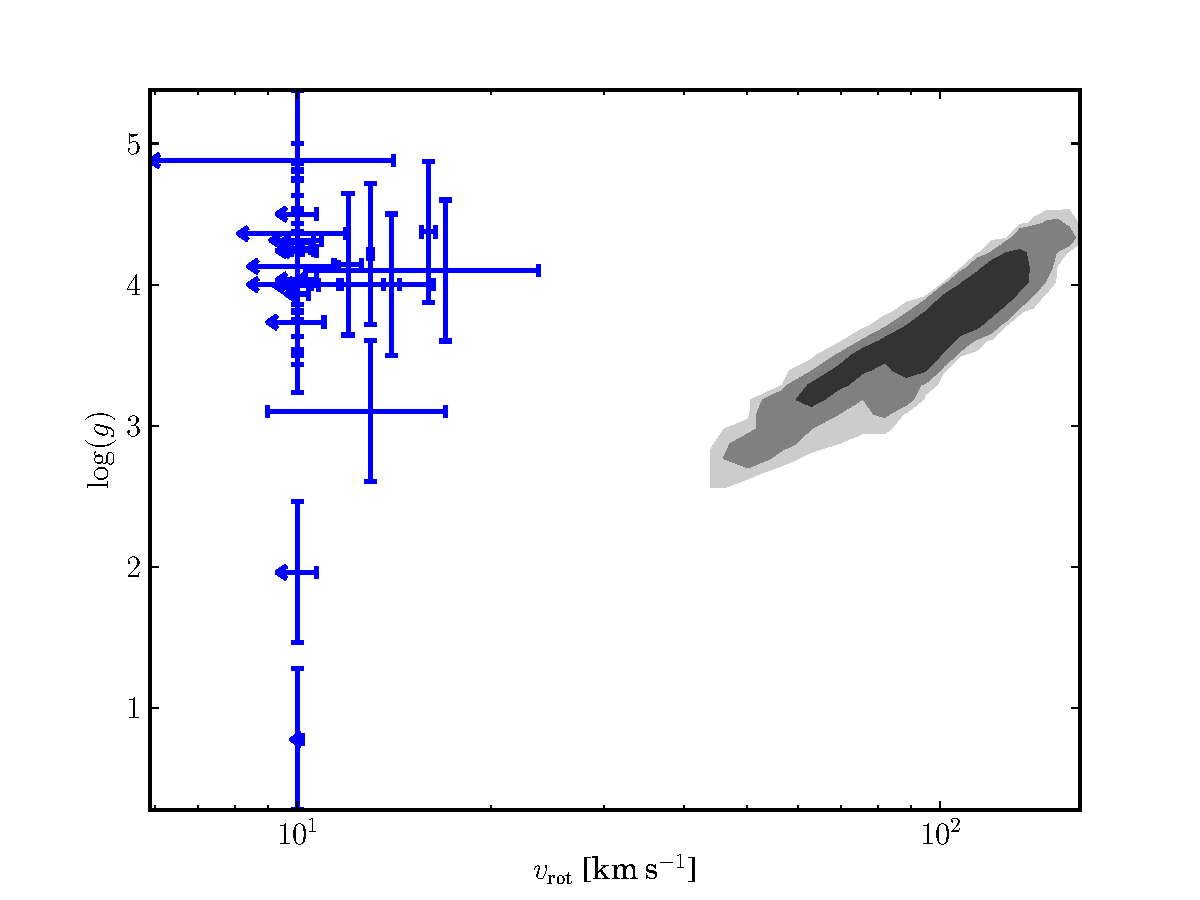
\includegraphics[width=\textwidth]{chapter_sn1006/plots/compare_vrot.pdf} 
   \caption[Comparison of rotation and surface gravity of SN 1006 candidates]{Comparison of the evolutionary state and rotational velocity of 55000 binary synthesis \glsentryname{sds} progenitors \citep[gray shades;data from][]{2008ApJ...677L.109H} with the measured rotation from this work. Due to the resolution of the spectrograph most of these stars only have an upper limit of the rotation speed of $\vrot=10~\kms$}
   \label{fig:han2008_vrot_compare}
\end{figure}


\begin{figure}[tb] %  figure placement: here, top, bottom, or page
   \centering
   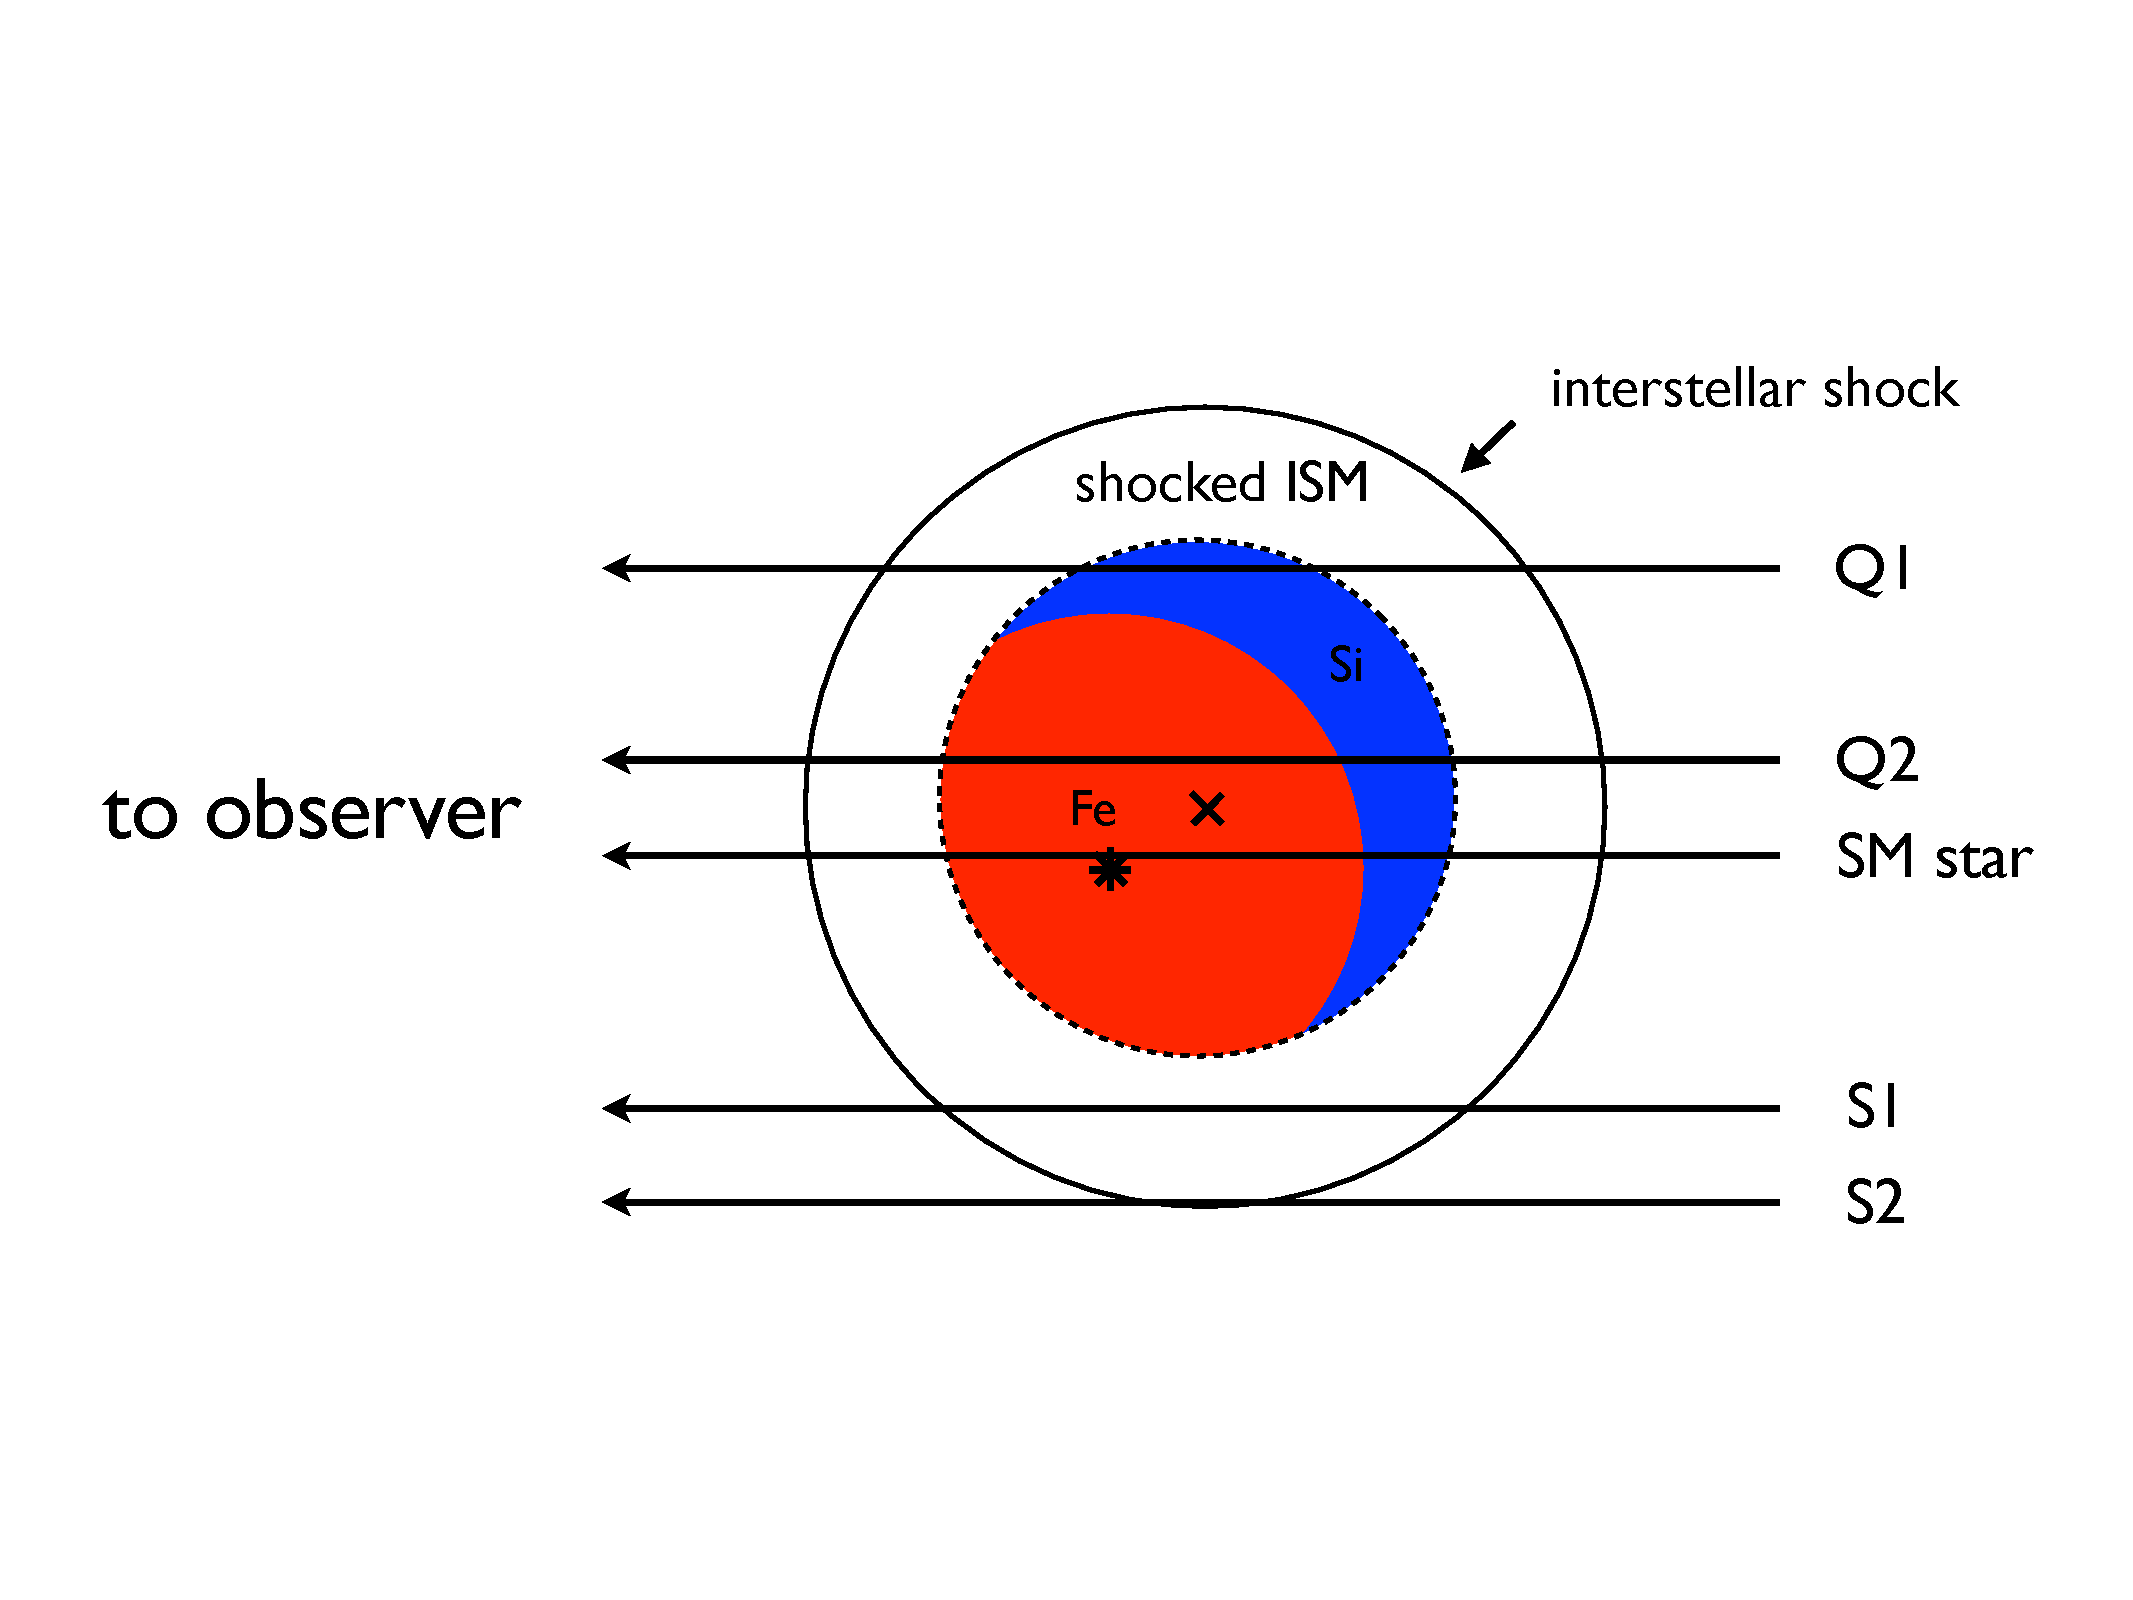
\includegraphics[width=\textwidth]{chapter_sn1006/plots/Winkler2005_probingsn1006_cropped.pdf} 
   \caption[Background UV sources probing the remnant]{Background UV sources probing the remnant. Figure adapted from \citet{2005ApJ...624..189W}}
   \label{fig:sn1006_uvprobe}
\end{figure}

The observations presented here for \sn{1006}{} are in conflict with the standard \snia\ donor star scenarios, which include accretion onto a white dwarf from a main sequence, sub giant, or giant companion. 
A few non-standard scenarios survive our observational tests. These include a helium white dwarf as a donor star (see Section \ref{sec:intro:subchandra}), which would not be detectable with our observations, although it is unlikely that a helium white dwarf would survive the explosion (priv. comm. R\"udiger Pakmor). The other possibility is that \sneia\ (or at least \sn{1006}{} and \sn{1572}{}) do not have donor stars, consistent with a \gls{dds}.

Another remnant that can be subjected to such an intensive search is Kepler (\sn{1604}). Kepler seems to be different from either \sn{1572}{} and \sn{1006}{}\ due to detection of interaction with the \gls{csm}. Observational facts of the Kepler remnant  as well as the description of the donor star search will be discussed in the conclusion of this thesis (Chapter \ref{chap:conclusion}).


% !TEX root =single_chapter_dalek.tex
\chapter{Automatic fitting of optical Type Ia Supernova spectra - the DALEK project}
\label{chap:dalek}

The last chapters (Chapters \ref{chap:sn1572_starg, chap:sn1572_hires, chap:sn1006_flames} were dedicated to the hunt for donor stars and did not use the measurements from the \snia-phenomenon itself. In this chapter we will describe the extraction of yields and energies from optical spectra. 

The two main sources of information in spectra, are the spectra themselves as well as their time evolution. There have been a few attempts to extract the details of the stellar explosions from one or two of these sources. All of them employ the technique of fitting the spectra using synthetic spectra. One of the main parts is the radiative transfer program that creates the synthetic spectra. There are several different radiative transfer-codes in the community. 


\cite{2000PhDT.........6F} wrote a very simple radiative transfer code called \synow. \synow is a highly parametrized code and thus is mainly used for line identification rather than actual fitting of supernova spectra. It runs 
The main code (henceforth \mlc) used in this work is an evolved code of  \cite{1993A&A...279..447M, 2000A&A...363..705M}. Compared to the \synow-code the \mlc-code calculates a radiative equlibirum tepmerature and uses this to compute internally consistent ionization ratios. In addition \mlc takes electron scattering into account as well as allowing for photon branching. 


Codes such as PHOENIX\cite{1999JCoAM.109...41H}, SEDONA \cite{2006ApJ...651..366K} and ARTIS \cite{2009MNRAS.398.1809K} are powerful 3D radiative transfer codes. They are the most "physical" codes available but take hours on supercomputers to produce spectra. These codes, however, are not feasible for fitting observed spectra as they take too long for each iteration. 

The main aim of this work is to automatically fit the torrent of observed spectra expected from the current and next generation of supernova searches. We opted to use the \mlc-code as it provides a good compromise between speed and "realism".

In section \ref{sec:mlc_intro}we will introduce a the inner-workings of the \mlc-code.  We will discuss the properties of the search space in \ref{sec:searchspace} and will introduce our optimisation strategies in \ref{sec:optimisation_strategies}. Finally we will conclude and give an outlook over future work for this unfinished project in section \ref{sec:dalek_conclusion}.

\section{The \mlc-Code}

The supernova can be divided in two different phases: the photospheric phase and the nebular phase. The \mlc-code only models the photospheric phase.
In this photospheric phase the supernova is treated like a sharp photosphere emitting a black-body spectrum with a fast moving layer of ejecta above that. 

There are many physical processes in radiative transfer. Of those the Bound-free opacity has the biggest contribution to the final spectrum. In addition, Thompson scattering is thought to have an important effect in redistributing the flux. As \mlc is required to run fast only Bound-Free opacity as well as Thompson scattering is implemented in the code.

Unlike stellar atmospheres in supernova ejecta one needs to consider the photon's doppler shift in relation to the surrounding medium. One major assumption that the code makes is that of the Sobolev approximation.  This means that at the interaction between photon and line resonance happens only at one specific point (thus disregarding any broadening effects to the line). For example a photon in free flight from the photosphere will be able to interact with resonance lines of lower and lower frequencies. The Sobolev approximation makes the code relatively fast 

Another assumption that \mlc makes is that the ejecta is in homologous expansion. This means that the velocity is a linear function of the radius:
\[
	v=  r / t.
\]

Combining both the Sobolev approximation with the assumption of homologous expansion yields this relatively simple formulat for line opacities:
\[
\tau_{ul} = \frac{\pi e^2}{m_e c}\, f \lambda t_{\rm exp} n_l\, \left(1 - \frac{g_l n_u}{g_u n_l}\right), 
\]
where $\tau_{ul}$ denotes the opacity going from the u-state to the l-state, $e$ is the electron charge, $m_e$ is the electron mass, f is the oscilator strength of the line, $\lambda$ denotes the wavelength, $t_exp$ the time since explosion, $n_x$ the number of atoms in the state x and $g_x$ is the statistical weight of the state x.
Both homologous expansion and Sobolev approximation have their caveats. In the case of homologous expansion it is thought to be a very good approximations after the first few minutes after the explosion. The main caveat for Sobolev approximation is that a line is not a delta-function, as assumed in the Sobolev approximation. If too strong bound-bound lines are close in frequency space it can lead to the first line shielding the second line. In summary for fast supernova fitting both approximations seem to still allow for a relatively well fitting spectrum.

We have discussed the propagation of the photons in the plasma but have not discussed the state of the plasma yet. The simplest assumption for the state one can make is local thermodynamic equilibrium. In this case the Boltzmann formula describes the level populations in a single ion:
\[
\frac{n_j}{n_{\rm ground}} = \frac{g_j}{g_{\rm ground}}\,e^{-(\epsilon_j - \epsilon_{\rm ground})/kT}
\]
Similarly we can calculate the ionization state using the Saha-equation:
\[
	\frac{N_j}{N_{j+1}} = n_e \frac{U_j(T)}{U_{j+1}(T)}\,C_I T^{-3/2} e^{\chi/kT},
\]
where $U_j$ is the partition function and $C_I$ is a constant. As the ionization likelyhood depends on the internal electronic state of the atom the partition function sums up over the different states:
\[
U_j = \sum_i g_{i,j} e^{-\frac{E_{i,j}}{kT}},
\]
where i describes the excitation states and j the ionization states. The other symbols have their usual meaning. 
The sum normally diverges slowly so one in practice just sums up until a highly excited state.

The \mlc\ uses the so called \textit{nebular approximation} which will calculate the excitation and ionization state of the SNe at nearly LTE cost. In this nebular approximation they introduce a dilution factor $W$. This is a purely geometrical factor. Treating the photosphere as a point source the factor would result in $W=1/r^2$ with r being the distance from the center. As the photosphere is expanded the dilution factor has a slightly more complex formula. An important point to note is that purely theoretical at the photosphere the dilution factor is 0.5.

The mean intensity for the supernova at a specific zone is given as:
\[
J = W B(T_R),
\]
where $T_R$ is the radiative temperature. The radiative temperature is estimated in the \mlc\ by matching the mean frequency of $B(T_R)$ with the mean frequency of the photon packets in the current zone (Wien approximation). W is chosen so that the frequency-integrated intensity matches the photon distribution. 

Using $W$ and $J$ one now can calculate the electronic and ionization states of the plasma:
\[
\frac{n_j}{n_{\rm ground}} = W \left( \frac{n_j}{n_{\rm ground}} \right) _{T_R}^{\rm LTE}
\]
and 
\[
\frac{N_j}{N_{j+1}n_e} = W \left( \frac{N_j}{N_{j+1}n_e} \right) _{T_R}^{\rm LTE}
\]


In the simplest case we can treat the ejecta as homogeneous in temperature and abundance. For now we will also assume a pure scattering line interaction. This means that the photon is absorbed at a resonance frequency and then instantaneously reemitted with the same frequency into a random direction. This in in contrast to photon branching which we will discuss later. 

We assume a time since explosion $t_e$, a photospheric velocity \vph, \lbol and an abundance distribution for the chosen elements. W7 \citep{1984ApJ...286..644N} is used in the \mlc\ as a density structure.

The one dimensional model is divided into multiple zones that each have the same abundance but a different density. 
Using an initial guess of \teff\ for the photosphere, one can calculate the plasma condition in each shell. 

The Monte-Carlo simulation begins. A photon packet is emitted with a random frequency and a random angle drawn from a Blackbody distribution $B(T)$. Each photon packet contains the same energy (more photons per packet in the red than in the blue). 
An event optical depth is calculated from a uniform random distribution so that $\tau_{\rm event}=-ln(z); z \in (0,1]$.  
In the next step there are three possible outcomes. We calculate the length of the path ($s_e$) that the packet can travel freely before $\tau_{\rm event}$ is equal to the Thompson scattering opacity $\tau_{\rm event} = \sigma_{\rm T} n_e s_e$. Next we calculate the same path length for the lines $s_l$ using as a target opacity $\tau_e + \tau_{\rm line}$. 
If both paths are longer than the path to exit the current zone, then the photon exits the current zone and a new Monte Carlo process begins. 
If however $s_e$ is the shortest then Thompson scattering occurs and the photon is assigned a new direction and a new $\tau_{\rm event}$ is drawn and the process begins anew.

In the case of line scattering the excited atom can de-excite through many lines. \mlc\ randomly chooses a downward transition for the whole packet (taking the appropriate weights into account). The number of photons in the packet is adjusted to ensure that the energy is conserved in the comoving frame. 

There are two possibilities for the final fate of the photon. Either it is reabsorbed into the photosphere or is emitted from the supernova. 

When initializing the state of the plasma one assumes an initial guess for the photon temperature. The Monte-Carlo simulation is run and records each packet status at the mid-point of each shell. This information is used to calculate a new photospheric temperature and an updated plasma condition (level population and ionization). 
This procedure is repeated until the photospheric temperature converges. Once convergence is reached the actual Monte-Carlo simulation begins. 

The final spectrum is not calculated using the escaping packets. Instead we calculate the optical depths using and then calculate the emerging spectrum using the formal integral. 
This has the advantage of reducing noise in the spectrum due to Monte-Carlo noise and gives very good results. 

A more detailed description of the code can be found in  \cite{1993A&A...279..447M,2000A&A...363..705M}.




\section{Manually fitting a Type Ia supernova}

When fitting manually there are several features that help guide the direction of the fit. We will attempt to explain by using a spectrum of SN2002bo (cite?????) 10 days before maximum. In this section we will only talk about fits with no abundance stratification. Stephan Hachinger has kindly provided his manually obtained best fitting parameters ( for the supernova at this stage (see Figure \ref{fig:sn2002bo-10_bf}).
Directly measurable are the redshift of the supernova (and implied distance) and the time of the spectrum relative to maximum. We assume calculate the time since explosion assuming a rise time of 19.5 days.
The other parameters are initialized using empirical data. 

\begin{figure}[htbp] %  figure placement: here, top, bottom, or page
   \centering
   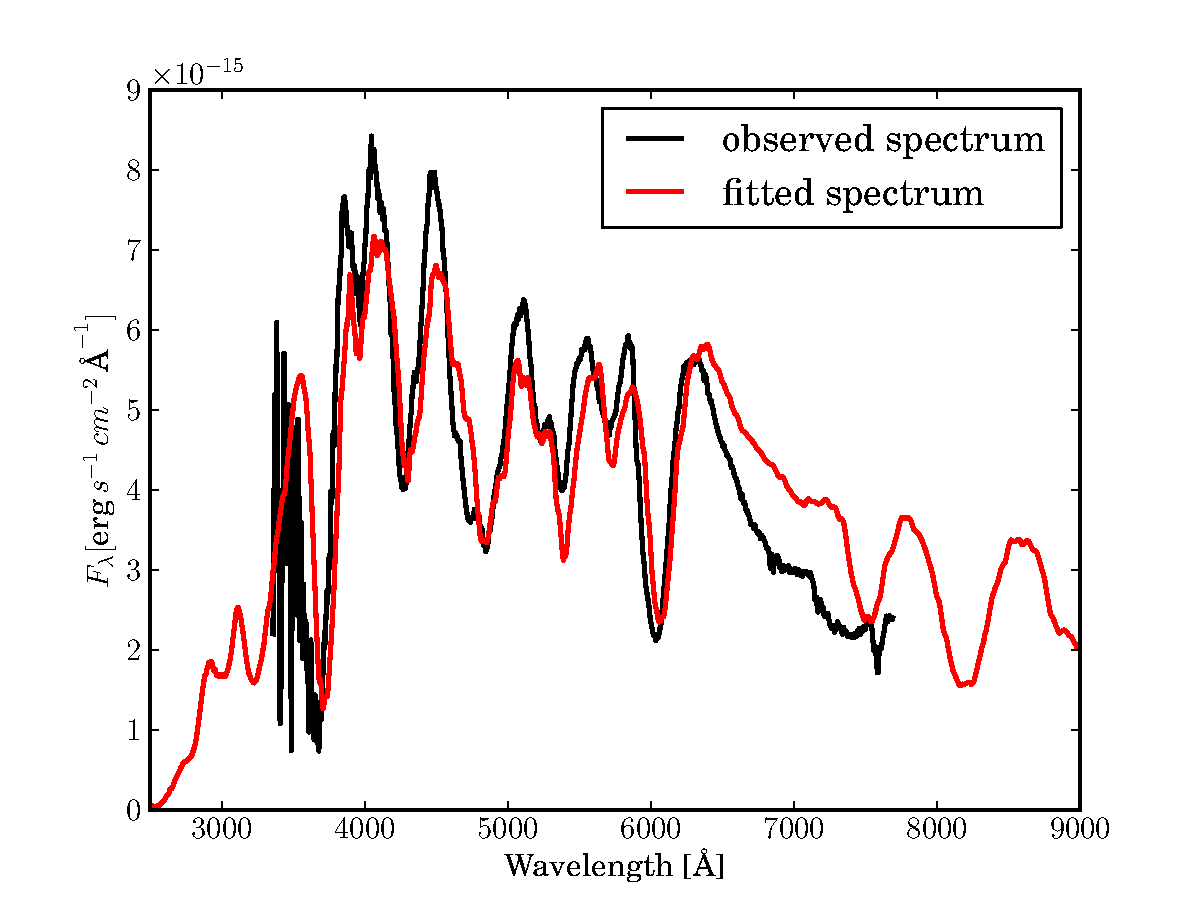
\includegraphics[width=\textwidth]{chapter_dalek/plots/bf2002bo-10.pdf} 
   \caption{example caption}
   \label{fig:sn2002bo-10_bf}
\end{figure}

The chosen fundamental parameters are $\loglbol=xx$, $\vph=xxx$. We have listed the non-zero abundances in Table \ref{tab:sn2002bo_perf_param}. 



The P-Cygni profiles of many features are easily visible. The Calcium line in the blue can be seen to be to blueshifted in relation to the model. This property is not unusual and is thought to come from high velocity component at the outer edge of the ejecta. The next major known discrepancy that can be seen is the excess of flux redwards of  $\approx 6200 \AA$.  This is a region that usually does not fit well as the underlying black body spectrum overestimates the flux in this region. When fitting manually often one tries to fit the depth the lines instead of the continuum.

There are three main parameters that have the most influence on the overall fit: Luminosity, photospheric velocity and abundance in iron group elements.

A large offset in \lum\ to the best fit paramater is easily visible as a large offset of the continuum (see Figure \ref{fig:sn2002bo_lum_offset}. Thus it is easy to constrain the parameter space in \lum\ initially. \lum\ also has influence on the temperature of the model through:
\[
L_{\rm bol} = 4\pi\sigma\, R^2\,T^4 = 4\pi\sigma\,\vph\,\texp.
\label{eq:lum_temp_relation}
\]

Velocity in astronomy is often measured using the doppler shift. In this case however it is hard to measure the photospheric velocity as lines are created at different depths and thus at different velocities. This smears out the line profiles which makes fitting velocities nearly impossible using this technique. 
The main impact of photospheric velocity is establishing the temperature given a luminosity. A model with a too high photospheric velocity will have expanded more than the real spectrum at that time and will be cooler. This results in a spectrum that is too luminous in the red and not luminous enough in the blue (see Figure \ref{fig:sn2002bo_vph_offset}). 
A secondary effect is that the ion population will be different to the actual supernova and the line spectrum differs.
\begin{figure}[htbp] %  figure placement: here, top, bottom, or page
   \centering
%   \includegraphics[width=2in]{replace} 
   \caption{example caption}
   \label{fig:sn2002bo_vph_offset}
\end{figure}
The initial abundances for each fit are determined by integrating the abundances above the photosphere in the W7 model \citep{1984ApJ...286..644N}.
The iron group element have a similar influence on the overall flux distribution as the photospheric velocity. 
As we assume no stable Cobalt and the input parameters for Nickel, Cobalt and Iron are $\Ni_0$ and $\Fe_0$ and calculate the abundances using radioactive decay. Ti and Cr have no easily identifiable single lines in the observed spectra, but provide line blanketing in the blue. We often lock their ratios and only use one abundance as an input parameter. 

These elements cause photons to be absorbed in the UV and be reemited in the red. A too high abundance will suppress the flux in the blue too much and will cause the spectrum to be over-luminous in the red (see Figure \ref{fig:sn2002_ige_offset}). Although physically different from the photospheric velocity, phenomenologically these are similar. 
The degeneracy is broken by identifiable Fe-Lines in the red part of the spectrum as well as the ionization balance determined by the temperature (influenced by photospheric velocity). 
This near degeneracy causes a very complex search space. 

There are six other abundances that are taken into account when fitting: Carbon, Oxygen, Magnesium, Silicon, Sulfur and Calcium. Among these Oxygen plays a special role. It does not have lines except the Oxygen triplet at 7778 \AA. In our fitting routine it acts as a buffer element and is assigned the remaining fraction that is left after all elements have been given abundances. 

The first element that is usually adjusted from its initial value is Calcium. The Calcium line is relatively easy to identify. Calcium also does not depend an awful lot on the right choice of temperature. One caveat however is that Calcium saturates at a certain point so if the observed line is close to that point one can only extract a lower limit for Calcium.

The next to be adjusted are Silicon and then Sulfur. Both of these elements are linked through nuclear synthesis and we don't expect there to be more Sulfur than Silicon. We also expect no less Sulfur than a third of Silicon. Silicon also provides an important measure for temperature through the ionization balance of doubly ionized Silicon to triple ionized Silicon (see Figure \ref{fig:sn2002bo_lineident}).


Magnesium has one strong feature near 4300 \AA, which constrains the Magnesium abundance. 

Doubly ionized Carbon has a line at $\approx 6300\,\AA$ which is often not present or very weak. 

Fitting the spectra involves first adjusting luminosity and then \ige s as well as photospheric velocity. This is followed by adjusting the other elemental abundances from the initial W7 values \citep{1984ApJ...286..644N}. After the elemental abundances are adjusted we readjust the luminosity, photospheric velocity and \ige again. This loop is continued until convergence is reached. 

One important factor to check is the value of the dilution factor $w$ at the photosphere. Theoretically we would expect this to be close to 0.5 if the fit is sensible. 

After having fit one spectrum we can continue to fit the other photpsheric spectra of the same supernova. We expect most parameters to increase or decrease monotonically (luminosity being the obvious exception). 

In summary, the fitting of a supernova is a complex procedure and requires a lot of practice. Our initial tests were using very simple methods like Newton-Raphson and other gradient methods. We quickly discovered the search space is too complex and evaluation time takes too long (each spectrum roughly one minute on a modern computer) to use these simple methods. 

 
\section{Genetic Algorithms}

Finding optimal solutions in complex search spaces is one of the main fields in numerical mathematics.  They have wide ranging applications in engineering, bio sciences and physical sciences. There have been several advances in the last decads to optimization. 
Among them is the  remarkable feat of ``solving'' the long-standing problem of the traveling salesman with simulated annealing \citep{Kirkpatrick13051983}.

\cite{Holland:1962:OLT:321127.321128}
Another major accomplishment was the development of evolutionary algorithms and subsequently genetic algorithms. The idea of an algorithm which imitates the principal of natural evolution was first introduced by ??? give story of rechenberg optimizing wind tunnel ??? Ingo Rechenberg \citep{Rechenberg1973}. These evolutionary algorithms have since become a sizeable subfield of numerical optimization. Genetic algorithms a subclass of evolutionary algorithms were then further developed by John Holland and David Goldberg \citep{citeulike:125978}.

When conquering the search space optimization algorithms have two (sometimes conflicting) goals: exploiting good leads while still exploring the search space sufficiently. Simple algorithms like Hillclimbing (randomly selecting a point in the neighbourhood and switch if it is ``better'' than the current one) will exploit good leads but will neglect to explore the search space. This often leads to be stuck at extrema. Whereas random searches are excellent at exploring the search space but will fail to quickly converge on an optimal solution. Genetic algorithms do strike the balance between exploration and exploiting the current best solution.
 """"
 maybe include:
 Dependent variables present special problems for optimization algorithms because varying one variable also changes the value of the other variable. For example, size and weight of the car are dependent. Increasing the size of the car will most likely increase the weight as well (unless some other factor, such as type of material, is also changed). Independent variables, like Fourier series coefficients, do not interact with each other. If 10 coefficients are not enough to represent a function, then more can be added without having to recalculate the original 10.
In the GA literature, variable interaction is called epistasis (a biological term for gene interaction). When there is little to no epistasis, minimum seeking algorithms perform best. GAs shine when the epistasis is medium to high, and pure random search algorithms are champions when epistasis is very high (Figure 2.5). cite haupt \& haupt (book on harddrive)
 """""""
Genetic algorithms are a heuristic search technique to find optimal solutions in n-dimensional search spaces. We will consider a function $f(\vec{x})$ with the multi-dimensional solution $\vec{y}$. In terms of genetic algorithms we call $\vec{x}$ genotypes and the solution vector $\vec{y}$ phenotype (similar to biology where the $\vec{x}$ describes the DNA sequence but the solution is can not be thought of as a vector). In addition we define a fitness function $g(\vec{y})=s$ where s is a scalar. It is our goal to choose the input parameters $\vec{x}$  to maximize $s$. 
Following the notation of \citep{Michalewicz:1994:GAD:184675} we introduce the population $P(t)$ with the individuals (sometimes referred to as genomes) $\{p_{1}^{t}, \dots, p_{n}^{t}\}$, where $t$ denotes the iteration. Each individual $(p_{i}^t)$ is a data structure consisting of a vector $\vec{x}_i$ and its corresponding fitness scalar $s_i$.  When we speak of evaluating $p_{i}^{t}$ we mean that we use $g(f(\vec{x}_i))=s_i$ to determine the fitness. A new population $P(t+1)$ is formed by choosing,  in the \textit{select step}, the more fit individuals. Some or all of the new population undergo transformations (recombine step). These transformations are called genetic operators. There are unary transformations, which create new individuals by small changes in single individuals called mutations. Higher order transformations called crossovers combine the traits of multiple individuals to form a next generation individual. 
After the new population has been created in the recombine step, it is evaluated and the \textit{select step} begins anew. 

This procedure is repeated until the best individual has reached a certain threshold fitness (see Algorithm \ref{alg:evol_program}). 



\begin{algorithm}
\label{alg:evol_program}
\caption{Structure of a genetic algorithm}
\begin{algorithmic}
\STATE $t \gets 0$\\
initialize $P(t)$\\
evaluate $P(t)$
\WHILE{(\textbf{not} termination condition)}
\STATE $t \gets t+1$\\
select $P(t)$ from $P(t-1)$\\
recombine $P(t)$\\
evaluate $P(t)$
\ENDWHILE
\end{algorithmic}
\end{algorithm}

To be solvable by a \ga the problem needs to meet the following requirements:
\begin{itemize}
\item a genetic representation of the search space (e.g. a vector)
\item a function that can calculate a fitness for a genetic representation
\item transformations that create a new population out of selected members of the old population
\item a method of creating an initial population
\end{itemize}


If these are fulfilled one can start constructing a \ga for the chosen problem. When constructing a new \ga for a problem there are multiple steps. First one needs to find a suitable genetic representation for each solution in the search space. 

\paragraph{Genetic Representation:}
There are two main ways to represent a genome: binary-encoding and value encoding (sometimes called gray encoding). Binary encoding was the form of encoding  used in early genetic algorithms. It offers significant advantages when trying to optimize very simple problems. 

In one-dimensional problems, for example, value encoding would only offer one gene, whereas binary encoding offers a number of genes depending on the requested precision of the value. 
There are however many problems with binary encoding. The so called \textit{hamming cliff} describes the problem that a simple bit-flip at one high encoding bit (occurring in some \ga\ operations) can dramatically change the encoded value \citet[e.g.][]{Chakraborty2003253}. This can improve covering of search space but also can hinder the code from converging quickly. When using binary encoding for many input variables the genomes can get incredibly large. \ga s have been shown to perform poorly for very large genomes. quicker convergence michalewicz page 82 chpter 5.5 

Value encoding often is a natural way to encode the parameters of a problem. In contrast to binary encoding the genetic operators are often much more problem specific. It seems that for the moment value encoding is the preferred method in many cases \citep[e.g.][]{Janikow1991Comparison,Wright91geneticalgorithms}.

Finally, an important encoding to mention (which does not apply to our example problem) is that of permutation encoding. In the famous case of the travelling salesman problem (henceforth \tsp) one tries to find the shortest route between n cities. In this case each city can only be visited once and the route must end in the starting city. There are many algorithms that can solve this problem. Brute force attempts scale with $O(n!)$ which make them unfeasible. A genetic algorithm can solve this problem by encoding the order (permutation encoding) in which the cities are visited in each genome. There are special genetic operators for permutation encoding. For the \tsp\ there are better algorithms like dynamic programming which can solve the problem with a complexity of $O(n^2 2^n)$ (see Figure \ref{fig:xkcd_tsp}).

\begin{figure}[htbp] %  figure placement: here, top, bottom, or page
   \centering
   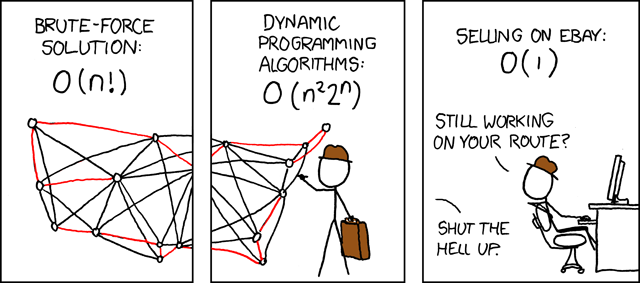
\includegraphics[width=0.7\textwidth]{chapter_dalek/plots/travelling_salesman_problem.png} 
   \caption{The death of the \tsp\ with the advent of online sales. (reproduced with kind permission by xkcd.com)}
   \label{fig:xkcd_tsp}
\end{figure}

In the case of a simple vectorized function or the \tsp\ once can now directly calculate the fitness value. In the case of our astrophysics example we need to first transform the genome (genotype) to a synthetic spectrum (phenotype) before being able to calculate the fitness.

\paragraph{Fitness Function}
Calculating the fitness of an individual is very dependent on the problem under consideration. In the case of our spectrum fitting problem we can simply calculate the root-mean-square for each individual. Finding a good fitness function in any optimization algorithm is one of the most complex tasks. It might not always be possible to find one fitness value that describes the problem but some problems might need many. This is generally referred to as multi-objective optimization and is an active field in \ga-research \citep{citeulike:1300532}. Fitness scaling applies a simple transformation to the fitness of all members of the population (e.g. a linear transform). Many selection processes are not able to accept negative and positive values for fitness so fitness scaling alleviates such a problem. In addition, it happens sometimes in early generation that a few individuals already have very high fitness. These "superindividuals" then dominate the selection process and subsequently reduce the genetic breadth  drastically. This can in later generations significantly hamper the progress of finding an optimal solution (such a problem was encountered in this work and is described in Section \ref{sec:geneticdalek}). 

In summary, fitness functions and scaling are a very crucial part of a successful algorithm. For a description of different scaling methods please refer to \citet{Kreinovich93geneticalgorithms} ??? select some introduction referebces from this paper???.

\paragraph{Initial Population}
The most basic method of selecting the initial population is to draw individuals uniformly and randomly from the entire search space. It depends then on the population size in relation to the search space size how well this search space is sampled. For a small population size and a large search space the \ga\ could very well find a local optimum rather than the global one. We have in our work chosen a population time which is roughly 15 times bigger than the number of genes. Choosing the initial population using prior knowledge will also improve the performance of the \ga. Rather than drawing uniformly random we would draw randomly from a probability distribution covering the search space. 

\paragraph{Selection process}
There are many different approaches for selecting individuals from the current population to create the next population. Before selecting individuals we can make coarse selection on the entire population. One selection that is often performed is that of \textit{elitism} in which a fraction of the fittest individuals is selected to advance to the next generation without being altered. On the other hand one can discard a fraction of the least fit individuals. These discarded members won't be used in the recombination step. The remaining population is called the mating population

After we have performed a coarse selection on the population we start with the recombination step. The first action in the recombination step is the selection of two or more individuals from the mating population and add them to a mating pool. In all our next examples we will assume a mating-pool with only two slots (similar to two parents in biological reproduction). Once the mating pool is filled a new individual is created by combining the genetic information of all members of the mating pool. 

There is a multitude of options for selecting members from the mating population and adding them to a mating pool \citep[for an overview see]{Goldberg91acomparative}. We will describe only a few of them. The most widely used of the selection algorithms is \textit{roulette wheel selection} (see Figure \ref{fig:roulettewheel}). \textit{Roulette wheel selection} is in the class of \textit{fitness proportional selection}. In addition to \textit{fitness proportional selection} there is \textit{rank selection}. In rank selection the fitness only influences the rank of the individuals (see Figure \ref{fig:rankselection}). The previous described fitness scaling and rank selection have similar effects. In \textit{tournament selection} we randomly select two individuals and compare those. The fitter of those two individuals is selected and added to the mating pool. 

There are multiple steps for creating a new population from the current mating population. First we select two individuals (or more) using our selection process (e.g. \textit{roulette wheel selection}) and place them in a mating pool. The reader should notice that the same individual can be in the mating pool twice! We create one or multiple new individuals (children) from this mating pool and place them in the new population. The current mating pool is disbanded and a new one is formed. These steps are repeated until the new population has the same number as the old population (minus the number of individuals that automatically advanced to the new population through \textit{elitism}). 
There are two main processes to create a new individual from a mating pool: crossover and mutation.
\begin{figure}[htbp] %  figure placement: here, top, bottom, or page
   \centering
   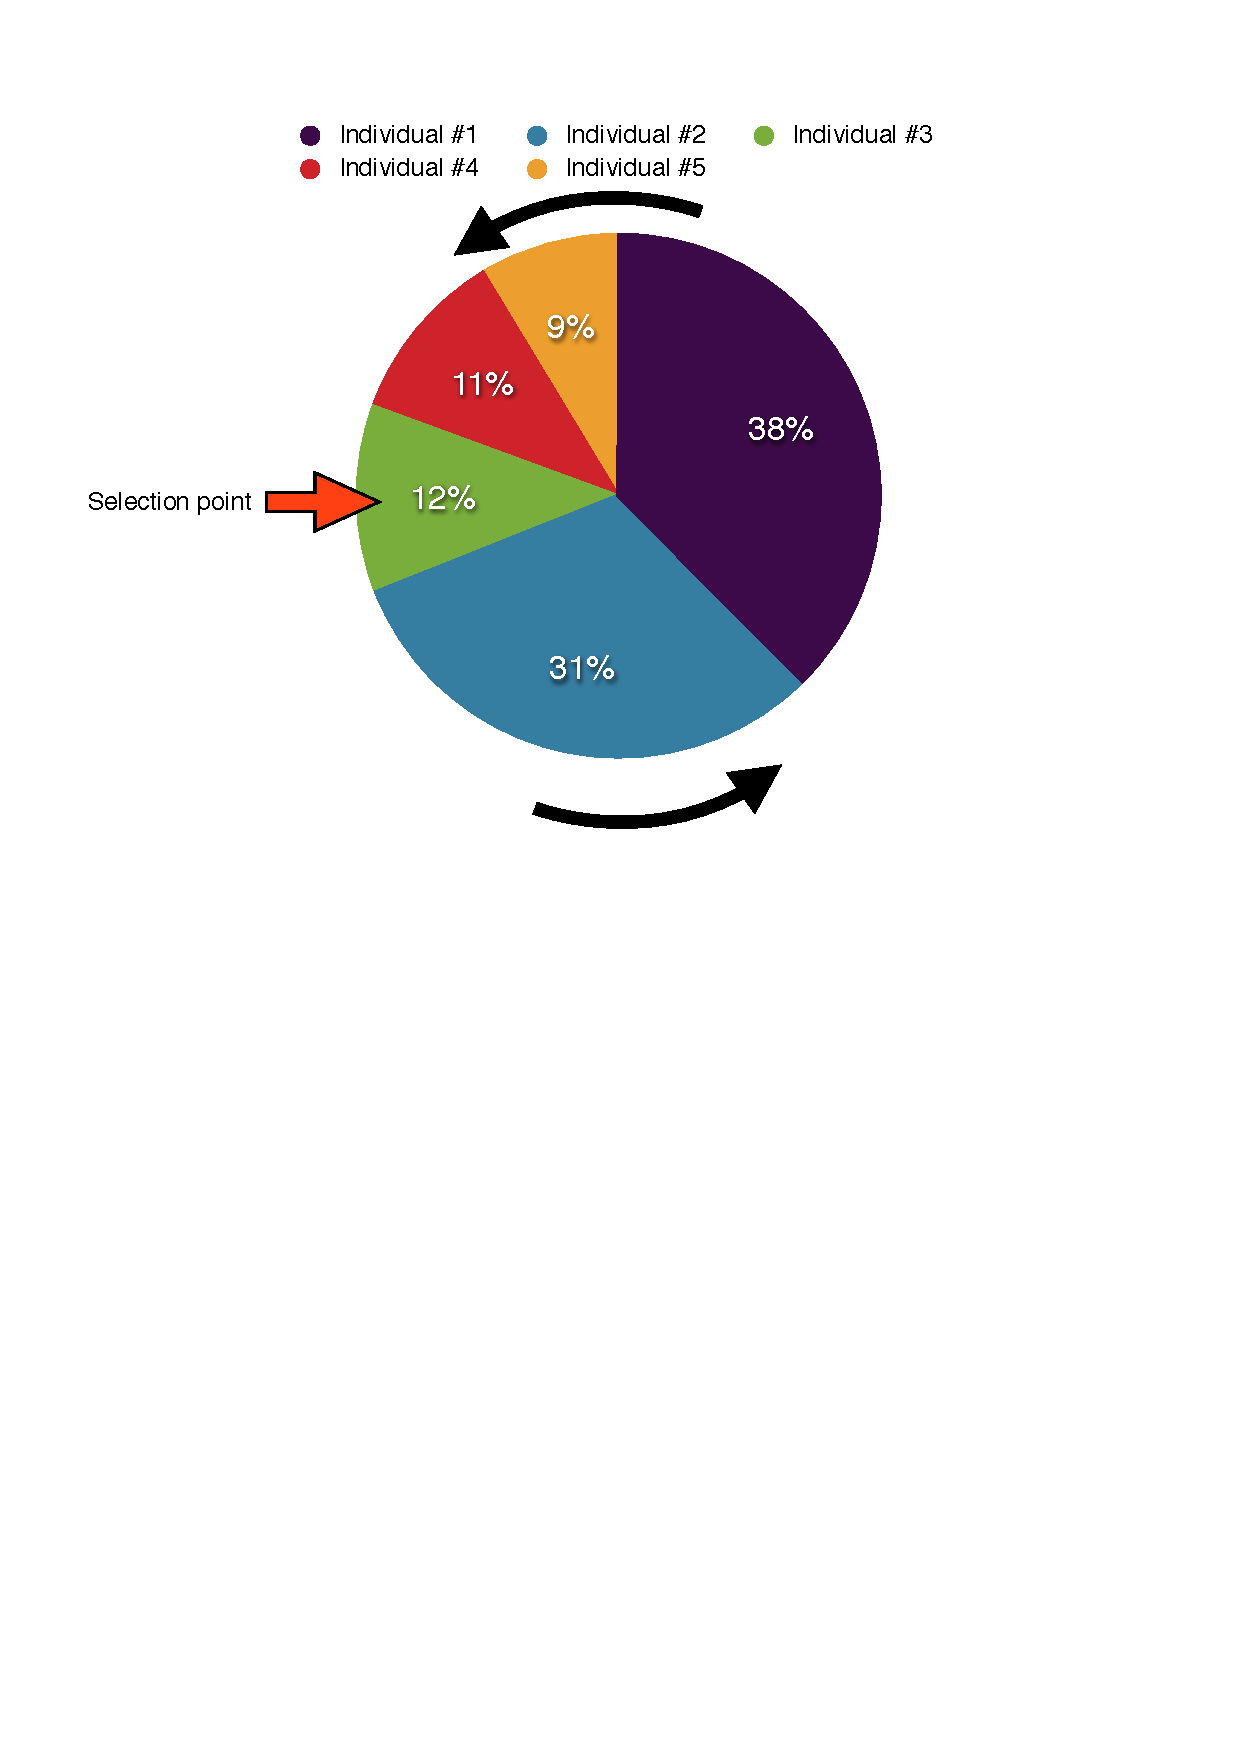
\includegraphics[width=0.7\textwidth]{chapter_dalek/plots/rws_cropped.pdf} 
   \caption{example caption}
   \label{fig:example}
\end{figure}

\paragraph{Crossover and mutation}
We assume a mating pool with two individuals. The simplest form of a crossover is the single-point crossover (see Figure \ref{fig:crossover}). A random integer $r \in [1,N-1]$, where N describes the number of genes per genome is selected. The new individual is created out of the first $r$ genes from the first parent and the last $N-r$ genes from the second parent. Now it is trivial to create a second child (using the same random number $r$) from the mating pool by just switching first and second parent. 
Two-point crossover is very similar to single-point crossover. Two random numbers are selected and the crossover occurs at these places (see Figure \ref{fig:crossover}). (N-1)-point crossover is also called uniform crossover. In that case each gene is selected randomly with equal chance from the parents.
Arithmetic crossovers use a function to calculate the new gene from each of the parent genes. For a value encoding this function could be the mean. For a binary encoding the function could be the \textit{and} operator. ???should I include example???
One can mix arithmetic and binary crossovers. For example we select the $r$ genes from the first parent and create the last $N-r$ genes by taking the mean of first and second parents genes. 
After the new child or children have been created through crossovers it is subjected to the mutation operator. There is a chance for each individual gene (often chosen to be less than 5\%) that it is altered. For bit encoding this altering is a simple inversions. There are many options for value encoding. For example one can add or multiply with a random number. 
Once this step is complete the children are added to the new population.

\subsection{A simple example}
We will illustrate the use of a \ga\ on a simple astrophysical problem. The task at hand is to fit an observed spectrum with a synthetic spectrum. The input parameters for this synthetic spectrum are\teff, \logg, \feh, $\alpha$-enhancement, \vrad and \vrot. The simplest genetic representation of this is simply a vector $\vec{x} = (\teff, \logg, \feh, \alpha, \vrad, \vrot)$. $\vec{x}$ is the \textit{genotype} of the individual. The resulting synthetic spectrum is called the \textit{phenotype}. 

For this relatively small number of genes a population size of 75 should suffice. The first step is drawing an initial population. We will draw uniformly randomly from the search space: $\teff \in [2000, 9000]$, $\logg \in [0, 5]$, $\feh \in [-5,1]$, $\alpha \in [0,0.4]$, $\vrad \in [-100, 100]$ and $\vrot \in [0,200]$. We compute the synthetic spectrum for each individual. The fitness of each individual is the inverse of the root-mean-square of the residuals between the observed and the synthetic spectrum. 
In the select step we will first advance 10 \% of the fittest individuals to the next population unaltered (\textit{elitism}). For the next population to be complete we need $75 - 8 = 67$ individuals which are created through mating. We select 2 individuals through \textit{roulette wheel selection} and place them in the mating pool. A single crossover point is randomly selected and the child is created. Before being placed in the new population the mutation operator is applied but has a very small chance to mutate any of the child's genes (in this case we choose 2\%).
This mating step (see Figure \ref{fig:example_mating}) is repeated 67 times. The new population now consists of the 8 fittest individuals of the old population and 67 new individuals created by mating. We will then start again to compute the synthetic spectrum and the resulting fitness for each individual of the new population. This loop is continued until one individual or a whole population has reached a preset convergence criterium.

\subsection{Convergence in Genetic Algorithms}
A key problem with all optimization algorithms is the premature convergence on a local optimum. The more complex the search space and the more interlinked the parameters are the more likely it is that traditional search routines will fail. \ga s are inherently better at bypassing local optima but are in no way immune to this problem. Premature convergence, as finding a local optimum is called in \ga-terms, is a well known problem 
A problem that is intrinsic to the \ga s is that for in traditional implementation they will never fully converge. The algorithm will get close to the optimum but due to continued mutation of the individuals the \ga\ will in most cases not reach it. To alleviate this problem some authors suggest switching to a different algorithm when close to the optimum solution, whereas others suggest changing the mutation rate over time \citep[see][and references therein]{citeulike:344183}.
A definite advantage of \ga s is their parallel nature. This makes it easy to explore large search spaces in the era of increasingly parallel computing. 

Although there are many advantages to using \ga s, one of the unsolved problems is determining a mathematical description for their convergence. The predominate schemata theory explains only a subset of the intrinsic complexity of \ga s.

\subsection{GA theory schemata theory}

The schemata-theory first described by \cite{holland1975} is one of the accepted theoretical interpretations of \ga s. There is some criticism and it is known that this theory only explains part of the complexity that are inherent to \ga s \citep[see ][ and references therein]{Whitley94agenetic}. 

\section{Genetic Algorithms to fit Type Ia Supernovae: The Dalek Code}
\label{sec:geneticdalek}
describe initial tries with newton raphson. 

Initial population. show vph graph. select from w7 integrate outwards. create children randomly; complex needs to work out and obey rules otherwise dead: describe process look at python code. ....

reference back to  parallelity and describe launching to multiple (non homogenious computers) simple fifo. 

fitness function describe chi**2 and then describe w-parameter and ir excess mention figure.

selection process rws; crossover uniform, mutation non-uniform different mutations for different parameters. child survival rate small at beginning.

describe principal evolution; show 2002bo different channels; population plot histtogram.
Fitting works sometime find good solution. discuss time and computer demand. discuss what has been tried

problems?

suggest that on the right way, now working with experts of genetic algorithms. describe differential evolution. 

ask james about machine learning techniques....

\section{Conclusion}



GA powerful tools, initially very good but require fine tuning for each problem.

A conventional, but not entirely accurate, interpretation of the NFL results is that "a general-purpose universal optimization strategy is theoretically impossible, and the only way one strategy can outperform another is if it is specialized to the specific problem under consideration"
http://ti.arc.nasa.gov/m/profile/dhw/papers/78.pdf

Continue on investigation with experts on GA. try some different approaches. Fast exploration of search space through grid and GA. 







%!TEX root = single_chapter_conclusion.tex
\chapter{Conclusions and Future~Work}
\label{chap:four}

\lettrine{A} lot of the aspects of \snia physics have been solved. We are very certain that this phenomenon is powered by the nuclear burning of degenerate Carbon/Oxygen fuel. The lack of hydrogen in the spectra of \sneia suggests that the progenitors are white dwarfs as they do not posses an extensive hydrogen envelope. The question that remains is: How and why do these objects explode?

\section{Single or Double Degenerate?}

The initial idea for this thesis was simple: High resolution spectroscopy and high precision astrometry of close and young remnant should reveal the suggested donor star. At this time the only viable scenario was the \sd-scenario. \dd-scenarios were almost unanimously believed to lead to accretion induced collapse and not a \snia. The first project was to confirm \starg\ as the progenitor of SN1572 and then move on and find the progenitors in both SN1006 and SN1604. 

The observations however started to show a completely different picture. The very unusual kinematics claimed for \starg \citep{2004Natur.431.1069R}, was only slightly unusual. The Besan\c{c}on model suggested the unusual velocity to be very usual if \starg\ was an uninvolved background interloper (see Section \ref{sec:sn1006:interloper}). We have realized that kinematics is definitley not conclusive evidence for a progenitor hunt, at most it is suggestive. 

The \sd-scenario in most cases suggests \gls{rlof} as the mass transfer. A consequence of this mass transfer mode is tidal coupling of the donor. Tidal coupling also implies that the rotation of the donor post-explosion is coupled to its escape velocity (see Section \ref{sec:sn1572_starg_rotation} and Figure \ref{fig:theorot}). For our search a serendipitous coincidence is that most low-mass stars do not rotate. Our work in Chapter \ref{chap:sn1572_starg} suggested that \starg does not have a unusually high rotation. Further work with better data (see Chapter \ref{chap:sn1572_hires}) established this. It is not entirely without caveats: the rotation might vanish post-explosion when the star puffs-up. In addition, the observable is not the rotation but the projected rotation, which is the intrinsic rotation diminished by a factor $\sin{i}$. Ironically, after the establishment of rotation as a donor star feature, we discovered a star with an unusually high rotation which was kinematically very normal (see Chapter \ref{chap:sn1572_hires}). No other stars in SN1572 and SN1006 (from preliminary analysis) show any unusually high rotation. 

Finding donor stars seems much harder than we initially thought. Both SN1572 and SN1006 don't have any strong candidates. We do acknowledge unusual stars in these remnants, but all of them have believable alibis which do not involve a \snia explosion. Only one star in the well studied remnant of SN1572 has so far eluded our spectroscopic scrutiny. This star (\stara 2 by our nomenclature) has an unusual proper motion according to our HST astrometry (see \ref{fig:propmot_sn1572_hires}). In addition it is located very close to the \xray center of SN1572. Unfortunately it hides 0.4\arcsec away from the 4 magnitudes brighter \stara (see Figure \ref{fig:stara2_overview}). This makes it impossible to obtain ground-based optical spectroscopy, but offers the possibility for challenging infrared observations aided by adaptive-optics. We are currently running a GNIRS-based campaign to obtain the fundamental stellar parameters, radial velocity and rotation. 

\begin{figure}[htbp] %  figure placement: here, top, bottom, or page
   \centering
   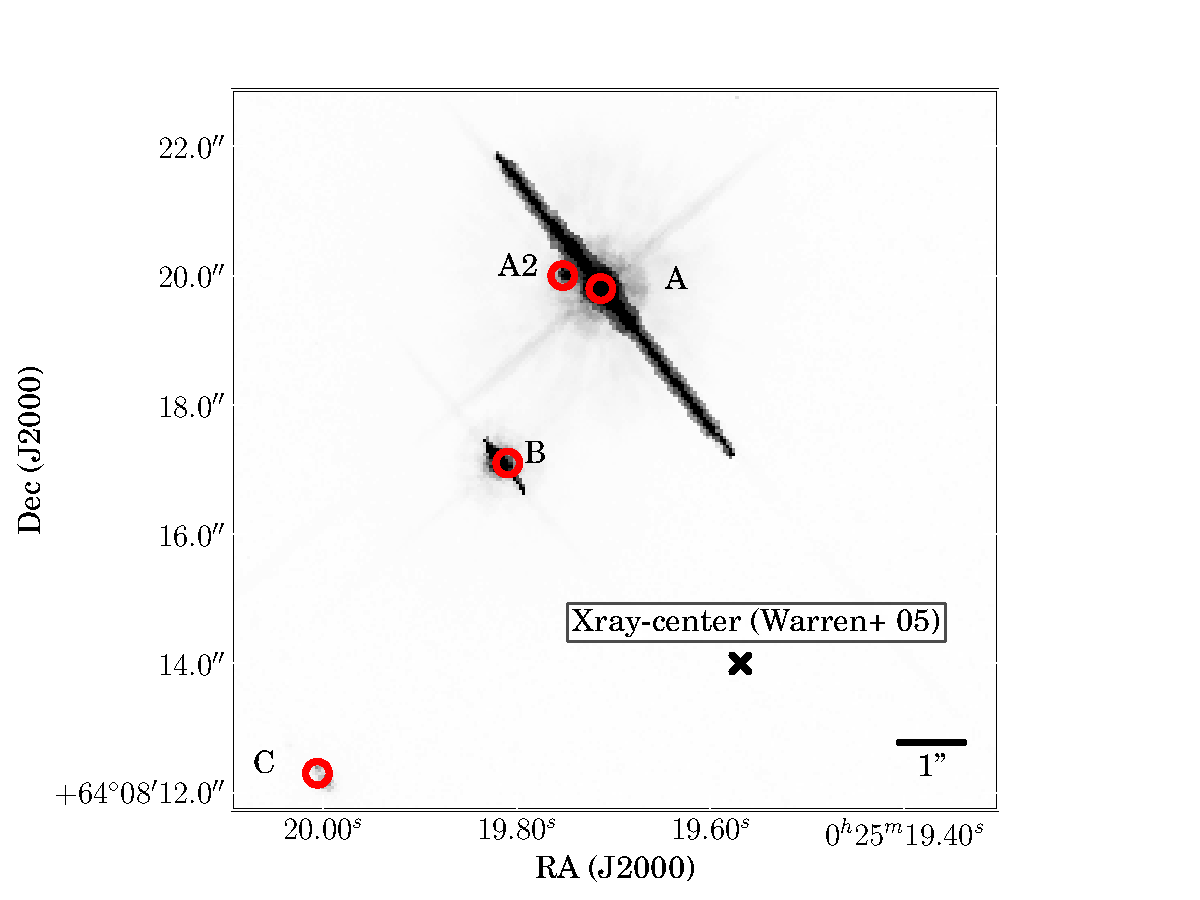
\includegraphics[width=0.7\textwidth]{chapter_conclusion/plots/overview_sn1572_a2.pdf} 
   \caption{Overview of inner region of the remnant of SN1572. All labelled stars except Star-A2 have existing high-resolution spectra. Tycho-A2 is located very close to Tycho-A (0.6\arcsec). Spectroscopy can only be obtained with adaptive optics in the infrared.}
   \label{fig:stara2_overview}
\end{figure}

The bottom line for both SN1572 and SN1006 seems to be: No bright progenitors. There are as always caveats, but we do think that with current theoretical knowledge and current instrumentation it is not worthwhile to scrutinize these remnants further. The only exception is to undertake photometrically deep observations of these remnants and look for a hot white dwarf. 

\section{The curious case of Kepler}

The last of the young remnants and the most distant one \citep[][estimates a distance of $\ge 6$\,\kpc]{2008ApJ...689..231V}.  The morphology of this remnant is not as clean and spherical as for SN1006 and SN1572 (see Figure \ref{fig:sn1604_observations}). For a long time SN1604 (Kepler's supernova) was also believed to be a \snib, but prominent iron emission in \xray spectra \citep{2007ApJ...668L.135R} suggests this event to be a \snia \citep{1995ApJ...444L..81H}. SN1604 also shows an abundance in nitrogen which is unusual for a \snia. \citet{1991ApJ...366..484B} and \citet{2003A&A...407..249S} suggest that the remnant itself posseses a very high systemic velocity of  $\approx 250\,\kms$. A recent study by \citet{2011arXiv1103.5487C} suggests that a \sd-scenario with an AGB star as a donor would explain all the observed peculiarities. They make the prediction that this star should be visible and very bright post-explosion. 

\begin{figure}[htbp] %  figure placement: here, top, bottom, or page
   \centering
   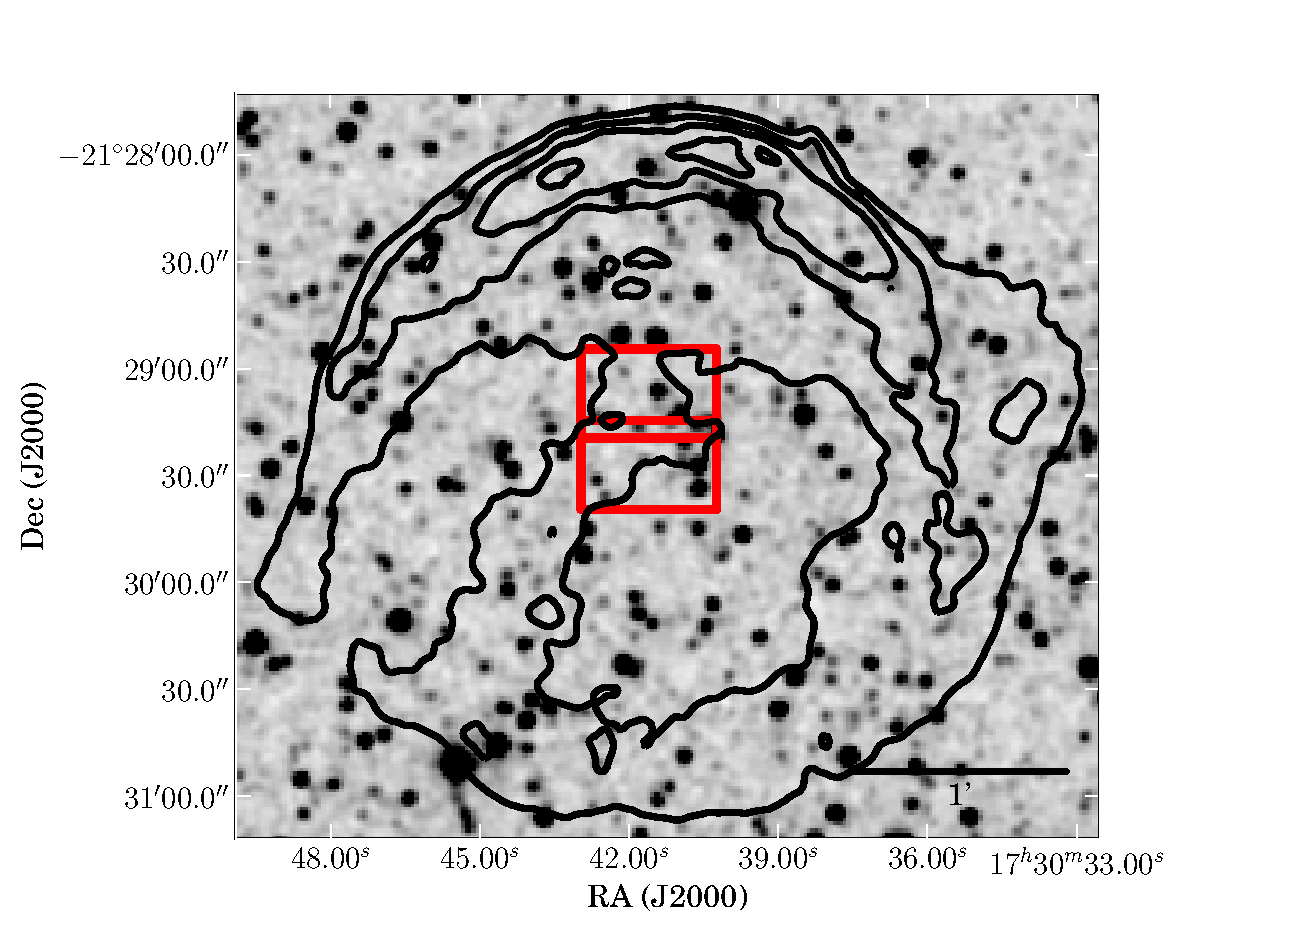
\includegraphics[width=0.7\textwidth]{chapter_conclusion/plots/sn1604_overlay.pdf} 
   \caption{VLA contours of Kepler's remnant (SN1604) overlayed on a \twomass\ image. The red rectangle show the overlapping north and south field of our WiFeS observing campaign.}
   \label{fig:example}
\end{figure}

We have obtained data with the WiFeS integral field spectrograph. The field of view for this instrument. is rectangular with dimensions of $25\arcsec \times 38\arcsec$. We have two overlapping fields that cover all stars at a projected velocity of 1300\,\kms (assuming a distance of 6\,\kpc). Extracting stellar spectra from our poor seeing data ($> 1.5\arcsec$) is technically challenging and we have not invested much time in this project.

\section{Divide et impera}

Maybe finding the progenitors of \sneia\ is too difficult using our current techniques. It might be much easier to employ the successful ``Divide et Impera'' - ``Divide and Conquer'' strategy. By asking many very small questions it might be easier to uncover on the truth than to try to solve this problem at once. We believe that one of these important questions is the mass at which \gls{cowd} explode. There are currently two main scenarios. The favored scenario is the explosion of the \gls{cowd} close to \gls{mchan} (1.38\,\msun). As shown in Chapter \ref{chap:intro} the burning of a 1.38\,\msun \gls{cowd} only produces the right abundance pattern when introducing a delayed detonation. When exploding a 1\,\msun \gls{cowd} this problem does not exist, a detonation of such a star produces the right optical photosheric spectrum. The main problem with these sub-Chandrasekhar mass explosions is that there exists no caveat free theory for the ignition yet. One key to find the explosion mass of any given \snia\ might be the abundance of stable in nebular spectra. In the Chandrasekhar mass case there should be more stable iron, in the case of a sub-Chandrasekhar mass there should be less.

\section{Dalek}

The title of this thesis suggests that \snia-progenitors and their explosions are mutually exclusive fields of research. In the previous section we have however shown that the mass of the white dwarf does have an influence on the yield. This mass is again linked to different progenitor channels. The analysis of spectra might not only help us constrain the elemental yields and explosion energies, but also give us insight into the progenitors. 

In Chapter \ref{chap:dalek} we describe a project to automate the analysis of \snia-spectra. The currently manual operated \gls{mlc}-code is ideal for automating as it strikes the right balance between speed and realism. We researched several numerical optimization strategies for this project before settling on \glspl{ga}. For now we have successfully fitted only one supernova spectrum. We are currently fine-tuning the algorithm and have enlisted the help of experts in the \gls{ga}-field. 

\section{Trouble in Paradise}

During the work of this thesis the field of \snia-research has changed significantly. When we started the donor star search there seemed little doubt in the community about the \sd-scenario. Over the recent years the \sd-channel has been seriously shaken and there has been some newfound support for the \dd-channel. The renaissance of the \dd-scenario, however often comes from the face that the merging of two white dwarfs doesn't provide as strong predictions as the \sd-scenario. This contention has reinvigorated the field of \snia progenitors and makes it a challenging and intriguing area to work in.

New transient and all sky surveys will soon start drowning us in a deluge of data. Currently the astronomical community is ill equipped to deal with such large amounts of data. This is not suprising as most astronomers are experts in physics and not data processing. This problem is not unique to astronomy, more and more fields are gathering much more data than is ever processable by individuals. We believe this is a great opportunity to start cross-disciplinary research. The fundamentals of science (e.g. pattern recognition) are definitley not unique to individual areas. New areas of science like eScience are trying to provide techniques and tools for scientists irregardless of the field. 

We have tried to conduct cross-disciplinary research in automatically fitting \sneia-spectra. Stephan Hachinger (the expert in manual fitting) and me initially have tried using the methods that were tought to us during our undergraduate years in physics (e.g. Newton-Raphson). These methods are still useful for very simple problems, however do not scale to today's highly non-linear problems with many co-dependant variables. Sam Inverso, a computer scientist working many in the area of neuro-science, joined us first and helped us do our first baby-steps in \glspl{ga}. His help has advanced the \gls{dalek} to its present state. In the last half year two new members have joined the team, whose research is in numerical optimization. They are very interested in applying their techniques to ``real world'' problems, which are scarce in the optimization community.

This work definitley tries to show: Multidisciplinary research is not only a buzzword, but can advance individual fields of science much faster than they could advance in isolation.





%% !TEX root =../thesis.tex
\chapter{SN1006}
\label{chap:three}

\lettrine[lines=4]{L}{orem} ipsum dolor sit amet, consectetuer
adipiscing elit. Mauris posuere, elit ac suscipit pulvinar, purus
felis vehicula purus, sed pellentesque arcu nibh eu turpis. Vivamus
volutpat convallis mi. Aliquam varius magna eu urna lacinia
dignissim. Proin venenatis tellus. Fusce pede dui, semper varius,
venenatis vitae, ultrices ac, dolor. Proin diam. Suspendisse eget
purus id leo accumsan scelerisque. Integer rutrum. Etiam risus nibh,
auctor eu, eleifend id, interdum ut, odio. Suspendisse
potenti. Praesent ultricies, mauris convallis vestibulum viverra,
nulla risus porttitor tellus, ut consequat velit nunc at nisi. Nulla
rhoncus nisl quis urna. Morbi sed nunc at tortor rhoncus
iaculis. Lorem ipsum dolor sit amet, consectetuer adipiscing elit. Sed
augue. Nunc molestie.

Maecenas at lectus id nunc bibendum placerat. Suspendisse cursus,
magna vitae blandit bibendum, nisi justo facilisis mi, at faucibus
elit urna id felis. Lorem ipsum dolor sit amet, consectetuer
adipiscing elit. Maecenas risus erat, ornare ac, varius nec, molestie
sed, nulla. Praesent sem urna, sollicitudin in, vulputate at, suscipit
vehicula, lectus. Integer mollis. Curabitur ornare, erat a facilisis
sagittis, risus nulla faucibus diam, at vehicula justo magna nec
urna. Pellentesque rhoncus, turpis eu facilisis molestie, diam ipsum
tristique massa, nec auctor risus diam quis metus. Lorem ipsum dolor
sit amet, consectetuer adipiscing elit. Fusce varius iaculis
neque. Aliquam erat volutpat. Cras sit amet nisi sit amet diam
imperdiet molestie. Quisque nec nisl. Cras nisi velit, pharetra sed,
cursus nec, euismod ac, turpis.

Morbi tincidunt, tellus nec dignissim congue, risus libero
sollicitudin tellus, sit amet porta magna libero sed ante. In id orci
eget nibh ultrices ultrices. Sed feugiat lobortis augue. Integer
nulla. Phasellus lacus diam, ornare id, ornare ut, dictum non,
velit. Ut egestas, risus quis placerat fringilla, nisl nunc tincidunt
ligula, et blandit dui diam vel sem. Morbi mattis turpis et purus
pellentesque accumsan. Mauris enim massa, sollicitudin at, lobortis
quis, ultricies sed, nunc. Pellentesque habitant morbi tristique
senectus et netus et malesuada fames ac turpis egestas. In in
arcu. Vestibulum ante ipsum primis in faucibus orci luctus et ultrices
posuere cubilia Curae; Donec eleifend molestie enim. Etiam justo. Sed
pharetra ultrices lectus. Mauris imperdiet varius purus. Aliquam
commodo adipiscing est. Pellentesque vitae odio fringilla pede viverra
tempor. Vivamus sed sem. Quisque molestie elementum lorem. Proin
aliquam odio vel sapien.

Quisque urna. Praesent scelerisque tortor nec elit. Pellentesque non
urna. Duis non sapien id nunc rutrum facilisis. Donec lectus ipsum,
ullamcorper vel, sollicitudin a, tempor a, sapien. Nam dui. In hac
habitasse platea dictumst. Integer eu ligula id lacus sollicitudin
sodales. Nam aliquam nibh vitae urna gravida rutrum. Aliquam erat
volutpat. Integer gravida mattis tellus. Etiam ipsum lacus, dapibus
id, volutpat eget, vestibulum vel, pede. In odio quam, viverra id,
adipiscing nec, consequat ut, orci. Nunc sit amet neque eu risus
dictum ultrices. Proin sem quam, ullamcorper ut, posuere at, tempus
eget, nibh. Cras ipsum. Phasellus bibendum purus eu enim. In hac
habitasse platea dictumst. Praesent eget leo ac sem congue sodales.

Nunc malesuada turpis vitae neque. Donec sollicitudin libero vel
nisi. Aliquam congue sem sed est. Integer eget ipsum. Nam eu
mauris. Aliquam vehicula tempor nulla. Duis faucibus ornare
elit. Vivamus nunc. Phasellus placerat, orci non blandit scelerisque,
neque urna faucibus justo, non gravida pede sem a urna. Sed eget arcu
eget enim pellentesque tincidunt. Cum sociis natoque penatibus et
magnis dis parturient montes, nascetur ridiculus mus. In in nulla sed
est venenatis sagittis. Mauris nibh orci, adipiscing in, blandit quis,
vulputate vitae, tortor. Quisque venenatis. Ut leo quam, pellentesque
vitae, dictum ut, vestibulum at, turpis. Aliquam id urna. Vestibulum
nunc mauris, facilisis sed, molestie quis, consequat non, dui.

Duis id metus et tortor viverra varius. Vivamus consequat. Sed
bibendum ultricies lectus. Pellentesque vulputate orci vitae
augue. Vivamus dignissim pharetra mauris. Lorem ipsum dolor sit amet,
consectetuer adipiscing elit. Vestibulum purus purus, commodo in,
consequat eu, lobortis eu, sem. Proin volutpat, pede eu imperdiet
bibendum, nulla odio lobortis eros, eu aliquet neque nunc eu
enim. Donec non nunc. Aliquam erat volutpat. Ut cursus fermentum orci.

Class aptent taciti sociosqu ad litora torquent per conubia nostra,
per inceptos himenaeos. Donec ante eros, porttitor vel, pellentesque
sit amet, laoreet ut, velit. Vestibulum sit amet turpis sed lorem
vestibulum vulputate. Maecenas sed orci in ante pharetra accumsan. Sed
id nibh. Pellentesque dapibus varius neque. Pellentesque habitant
morbi tristique senectus et netus et malesuada fames ac turpis
egestas. Nullam ultrices augue. Lorem ipsum dolor sit amet,
consectetuer adipiscing elit. Etiam convallis placerat
tortor. Suspendisse potenti. Mauris porttitor, justo et mollis
dapibus, dui nunc accumsan dolor, quis sollicitudin est nisi at
libero. Donec sollicitudin eros sed neque. Nunc at quam.

Donec id arcu. Sed vel sapien sit amet metus vestibulum
fringilla. Etiam fringilla ligula at arcu. Donec bibendum sem et
quam. Nam diam mauris, malesuada vel, placerat a, fermentum sit amet,
lectus. Cras venenatis justo nec leo. Aliquam vulputate erat. Cras
turpis. Cras gravida. Aliquam erat volutpat. Sed porta pretium
ligula. Mauris viverra, nisi euismod vulputate lobortis, est tortor
consectetuer arcu, at congue quam ipsum sit amet sem. Cum sociis
natoque penatibus et magnis dis parturient montes, nascetur ridiculus
mus. Mauris eget dolor.

Suspendisse pulvinar. Suspendisse felis nisl, mattis sed, facilisis
at, laoreet vitae, magna. Suspendisse potenti. Pellentesque et ligula
vel mauris suscipit vestibulum. Phasellus eros sem, volutpat at,
feugiat ut, aliquam sed, augue. In hac habitasse platea
dictumst. Suspendisse suscipit. Cum sociis natoque penatibus et magnis
dis parturient montes, nascetur ridiculus mus. In lectus dolor,
commodo non, ultricies eu, scelerisque at, orci. Nulla
semper. Suspendisse potenti. Donec orci diam, pellentesque tristique,
tempus eget, tincidunt in, dolor. Maecenas tristique vehicula
risus. Integer vitae nisi. Aenean sed enim eu nisl suscipit
scelerisque. Integer non metus. Donec dui erat, bibendum eu, suscipit
eu, facilisis non, erat. Morbi dapibus pede id justo. Fusce lobortis
volutpat enim.

Morbi leo turpis, facilisis in, ultrices vel, adipiscing ut,
erat. Praesent ligula. Maecenas quis velit in orci adipiscing
aliquam. Quisque at pede. Integer at odio. Pellentesque feugiat tellus
sed risus. Mauris et turpis. Nam sodales. Suspendisse mollis tincidunt
sapien. In ac sapien et purus sollicitudin ultricies. Integer eget
sapien quis ligula commodo egestas. Nulla aliquam, odio sed tincidunt
blandit, pede dolor gravida nunc, nec condimentum lorem nulla eget
dui.  




%
%%% BACK CONTENT:
%
\cleardoublepage
% for back matter, plain page style with no head/foot rules
\fancypagestyle{plain}{
\fancyhf{}
\fancyfoot[RO]{\bfseries \thepage}
\fancyfoot[LE]{\bfseries \thepage}
\renewcommand{\headrulewidth}{0pt}
\renewcommand{\footrulewidth}{0pt}
}
\pagestyle{plain}
%
% bibliography
% \phantomsection\addcontentsline{toc}{chapter}{Bibliography}
\printglossaries
\bibliographystyle{astroads}
\bibliography{thesis}
%
% appendices
\phantomsection
\appendix
%\appendixpage
% !TEX root = ../thesis.tex
\chapter{Linear interpolation in N~Dimensions}
\label{chap:ndinterp}

Interpolation is one of the most common operations in astronomy. Resampling spectra to a different wavelength grid, projecting images or interpolating physical quantities in n-dimensional fluid dynamics simulation are all examples of interpolation.
Interpolation can be described as a special case of curve fitting which requires the function to go through all points. 

In one dimension interpolation is relatively easy and there exist multiple methods. The simplest method is nearest-neighbour interpolation in which the algorithm picks the closest neighbour point to the point to be interpolated. 

Linear interpolation is one of the most common methods of interpolation. The two neighbouring points of the point to be interpolated are found and their slope and offset is used to obtain the interpolated point.

A more sophisticated approach is the spline-method of interpolation. Splines are piecewise polynomials of n-th degree whose first and second derivation are the same at the data points.

In one dimensional space there exists an abundance of interpolation methods. This multitude of options decreases rapidly with increasing number of dimensions. 
We will focus on the implementation of linear interpolation in N-dimensions, although there are a few other options like nearest neighbour interpolation and radial basis function.

For our linear interpolation we have opted to use \deltri\ as a interpolation method. The interpolation involves multiple steps to arrive at an interpolation solution: At first a \deltri\ is performed on the existing points. As a next step we need to find the simplex(geometric structure; a triangle in two dimensions) that contains the point to be interpolated. 
Finally we will use the barycentric coordinate system of the simplex to perform the actual interpolation.






\section{Delauney triangulation}
\label{sec:delauney_tri}
A triangulation is the process of connecting all points in a set with straight lines without any two lines crossing (see Figure \ref{fig:delauney_example}). It is obvious that there many ways for a set to be triangulated. All triangulations however have the same outer boundary called the convex hull. One special kind of triangulation is the \deltri. The \deltri\ can be defined a various abstract ways and has intriguing properties.

\begin{figure}[tb] %  figure placement: here, top, bottom, or page
   \centering
   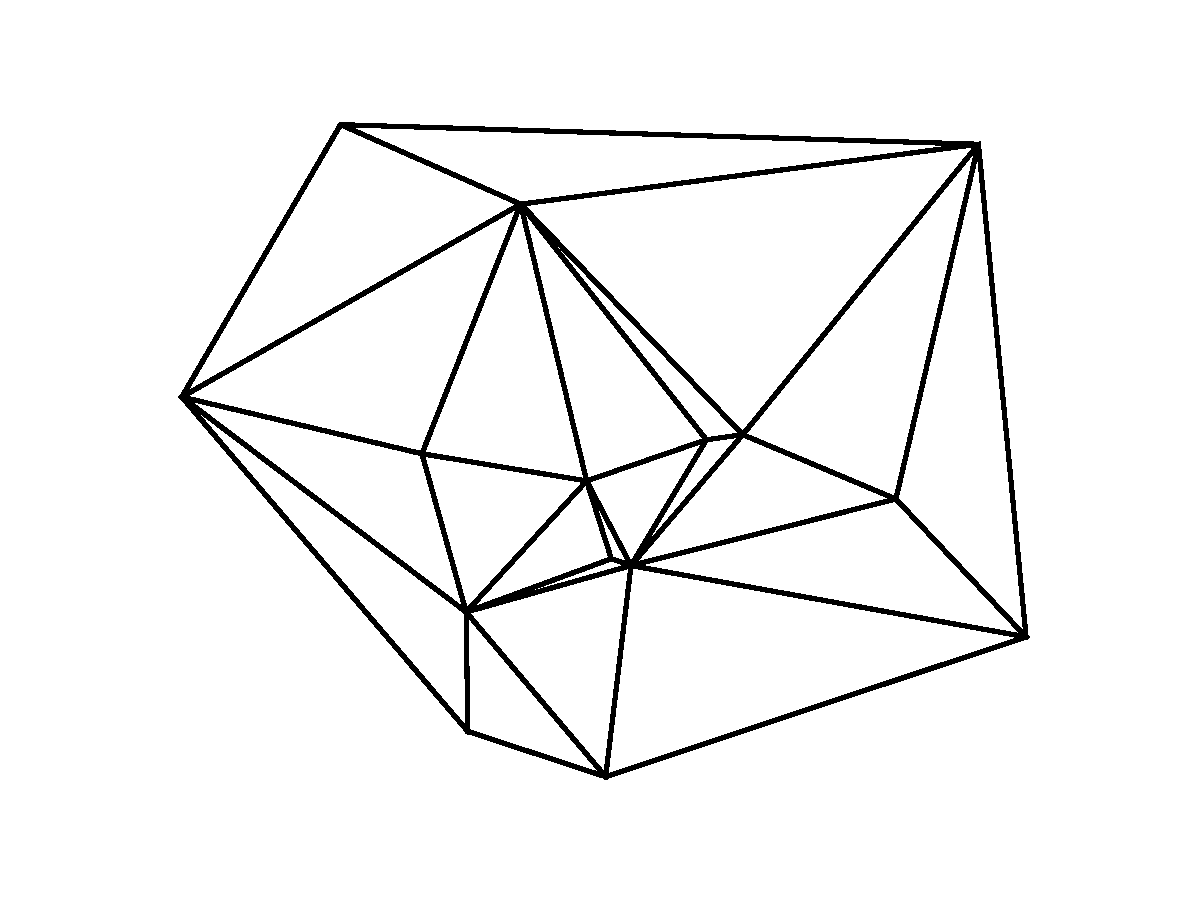
\includegraphics[width=\textwidth]{chapter_ndinterp/plots/simple_delauney.pdf} 
   \caption{\deltri\ of 20 points in two dimensions.}
   \label{fig:delauney_example}
\end{figure}

For a description of the process we will limit ourselves to two dimensions. This process is expandable to n dimensions in which the triangles become geometric structures called n-simplices.
One such defintion is that the circum-circle (circle going through all three points of the triangle) of each triangle must only contain three points. Figure \ref{fig:delauney_allowed}, a simple example, shows one \textit{legal} triangulation and one \textit{illegal} triangulation. One can see in the \textit{illegal} triangulation that the circum-circles of both triangles contain more than tree points. By doing a simple "\textit{edge-flip}" one arrives at the \deltri. In addition this ensures that the triangulation gives the largest minimum angle for both triangles. 

\begin{figure}[tb] %  figure placement: here, top, bottom, or page
   \centering
   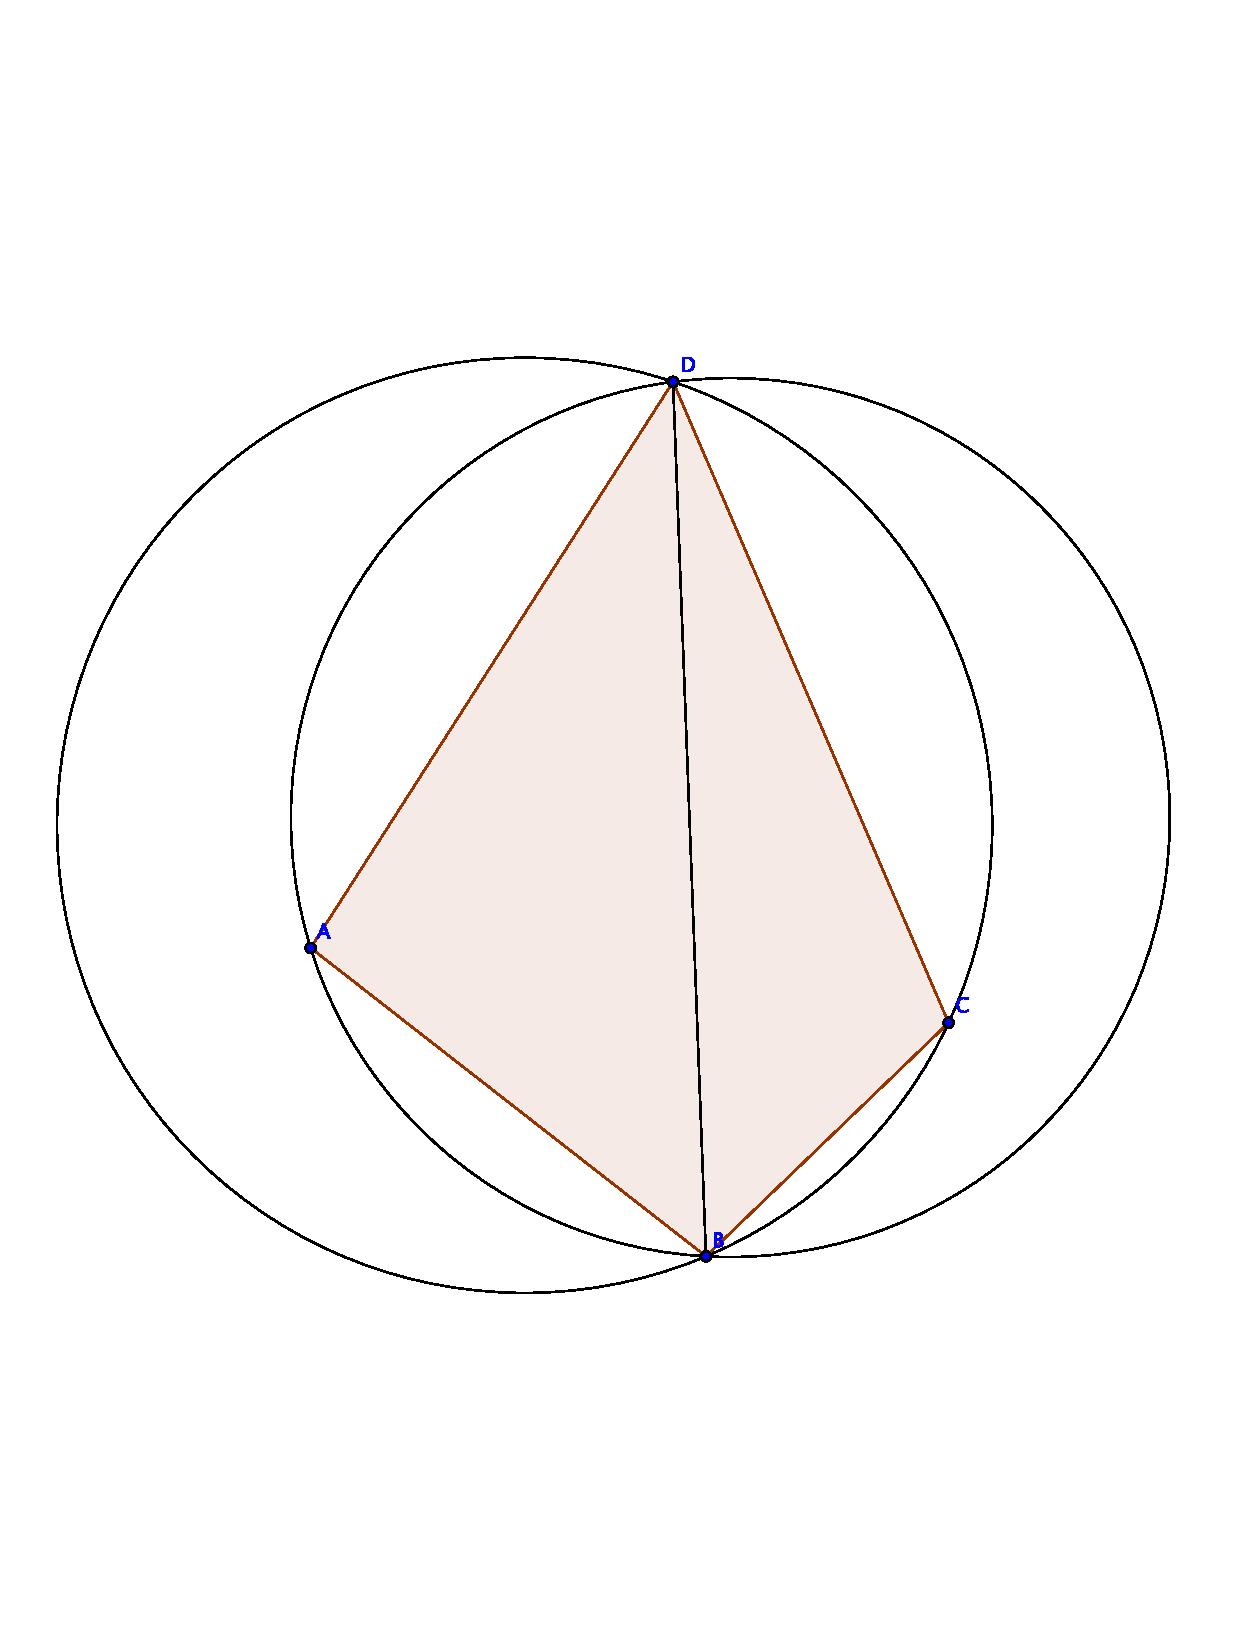
\includegraphics[width=.45\textwidth]{chapter_ndinterp/plots/illegal_triangulation.pdf} 
   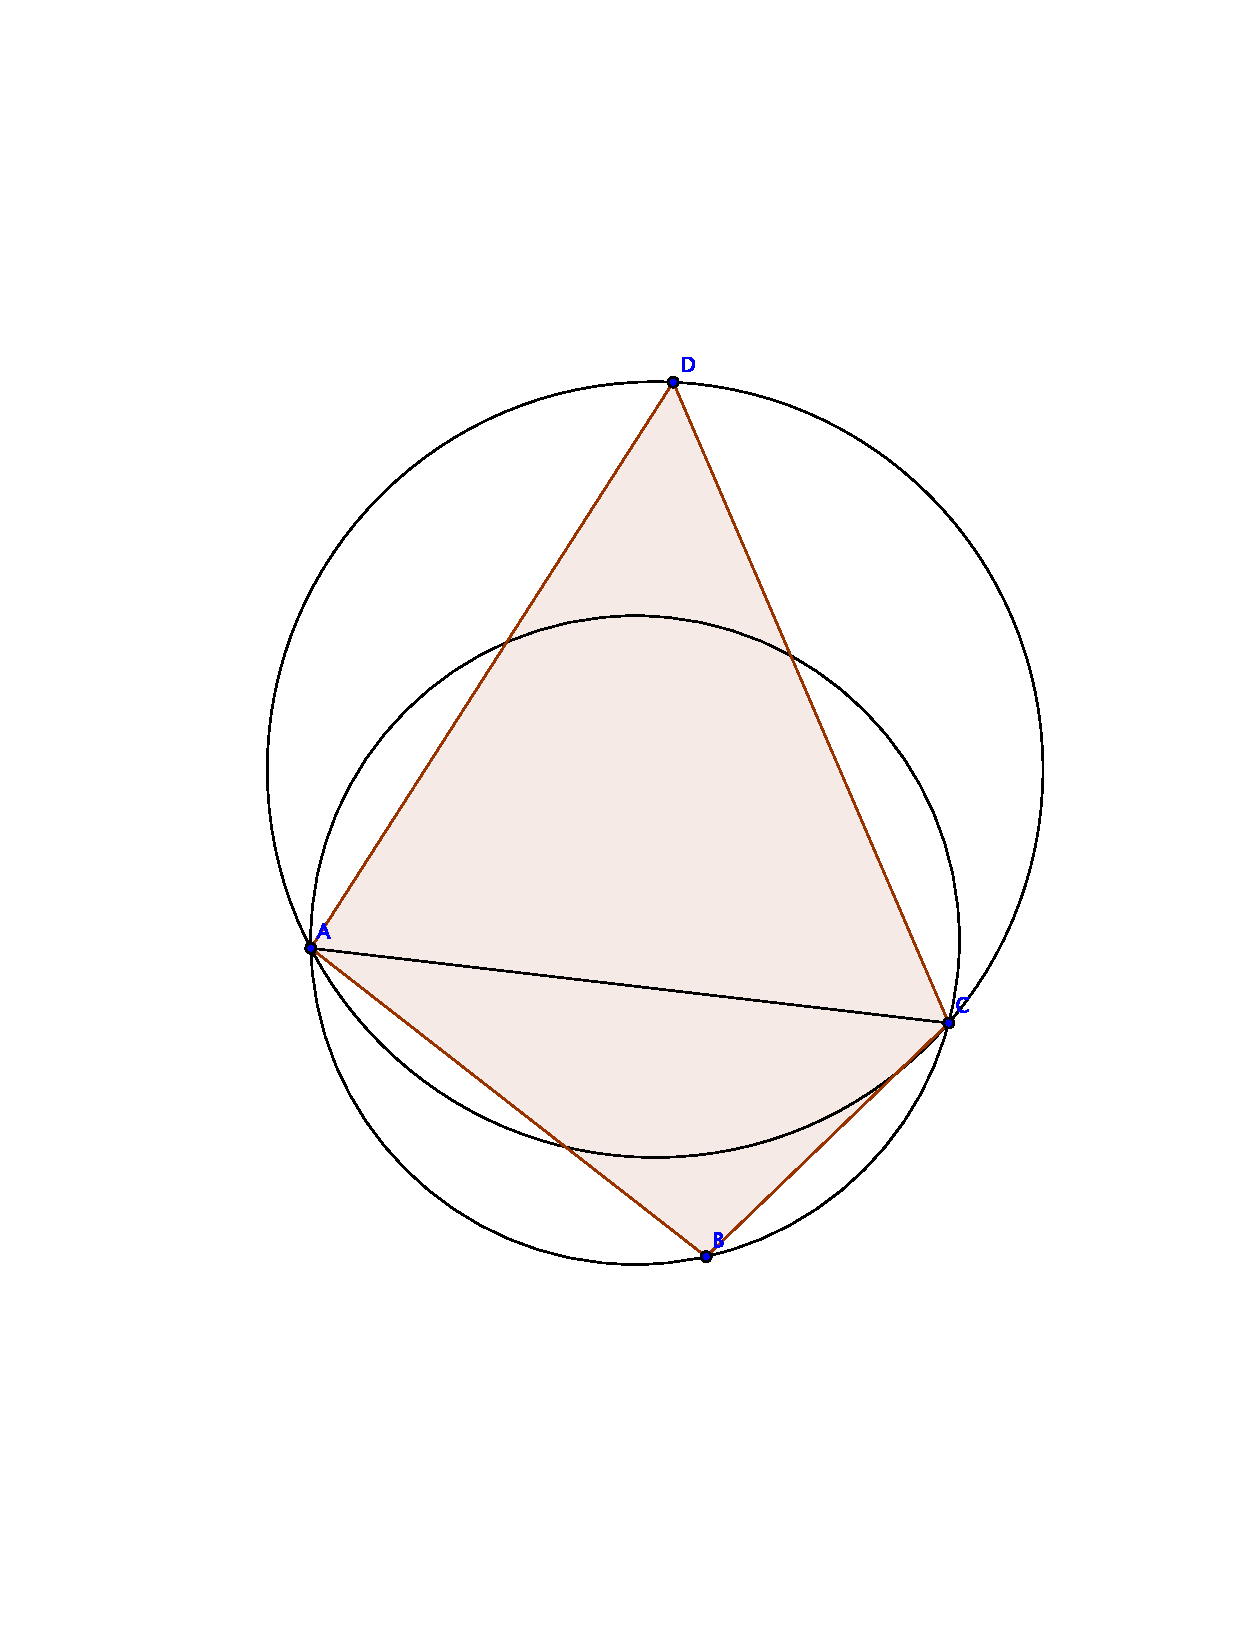
\includegraphics[width=.45\textwidth]{chapter_ndinterp/plots/edge_flip.pdf} 
   \caption[Change from a `illegal' triangulation to a \deltri]{The left figure shows an `\textit{illegal}' triangulation of the 4 points. Both circles include all the points. With a so called edge flip one can arrive at a `\textit{legal}' triangulation.}
   \label{fig:delauney_allowed}
\end{figure}
\deltri\ and convex hulls have a very interesting relation. It is possible construct the \deltri\ in n dimensions from a convex hull of the points projected on a paraboloid in n+1 dimensions.
Figure \ref{fig:delauney_projection} shows an example of a \deltri\ in two dimensions constructed from the convex hull in three dimensions. To project the points onto the paraboloid one just square sums the coordinates n dimensions and uses this as the coordinate for the point in n+1 dimensions. 

\begin{figure}[tb] %  figure placement: here, top, bottom, or page
   \centering
   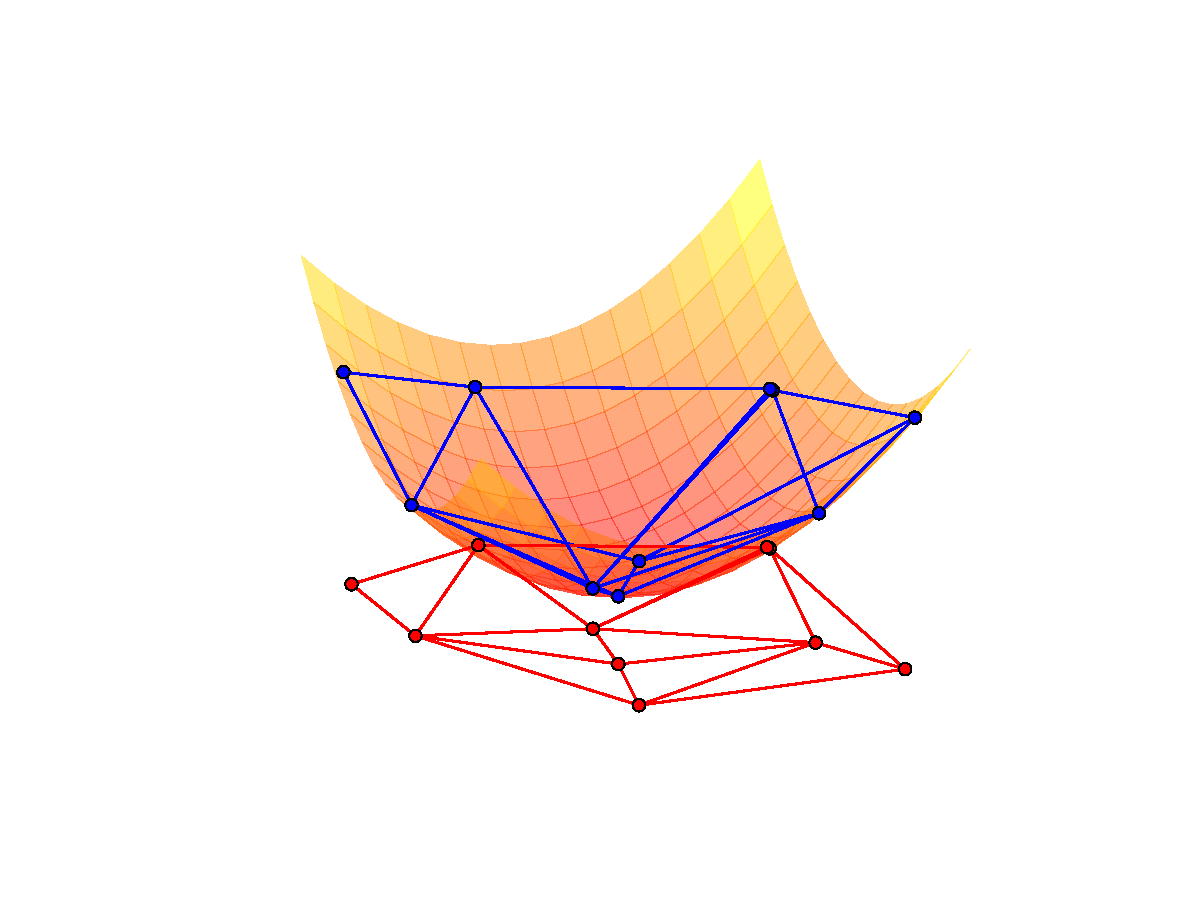
\includegraphics[width=0.49\textwidth]{chapter_ndinterp/plots/delauney_project_left.pdf} 
   \hspace{-1.5cm}
   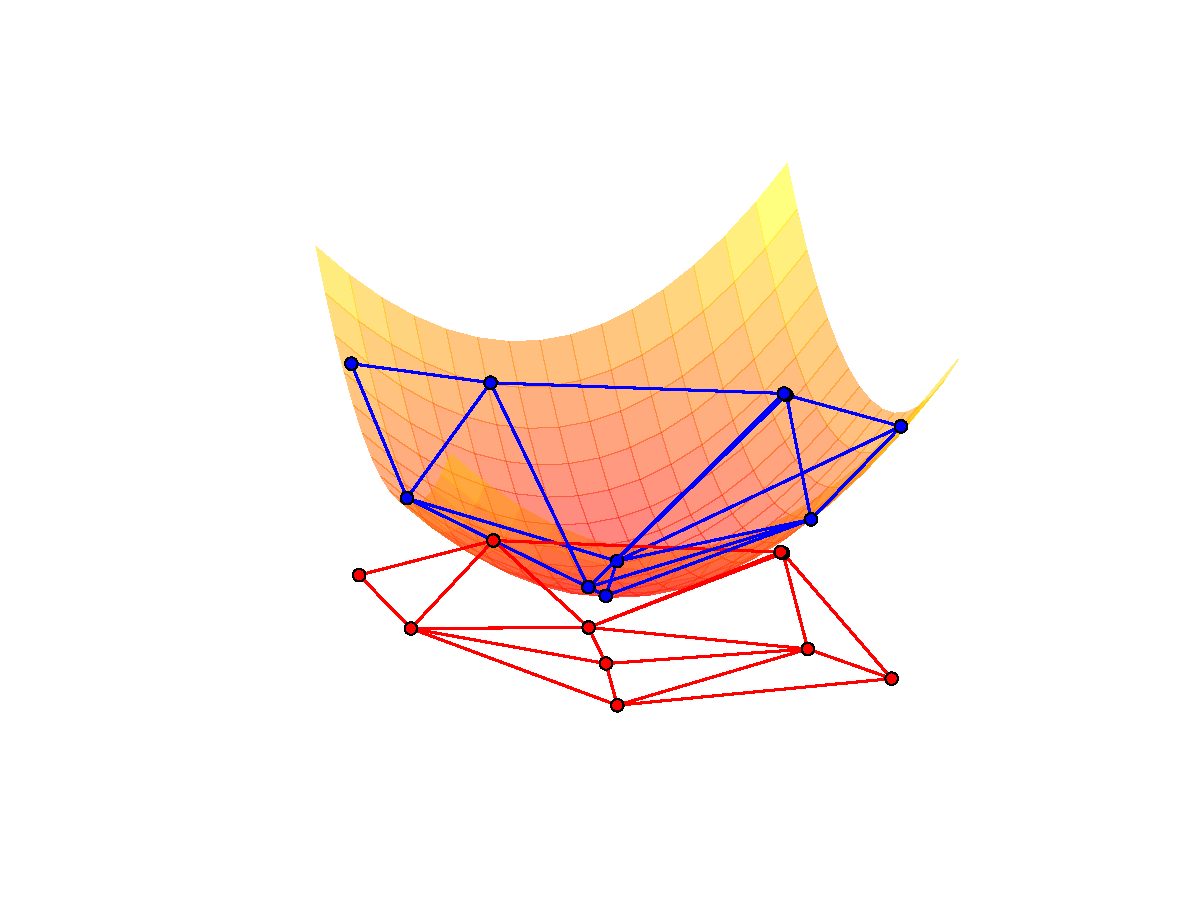
\includegraphics[width=0.49\textwidth]{chapter_ndinterp/plots/delauney_project_right.pdf} 
   \caption[Stereogram of the projection of the convex hull in three dimensions]{Stereogram \citep[produced using a method described in ][]{Vogt11} of the projection of the convex hull in three dimensions to form the \deltri\ in two dimensions.}
   \label{fig:delauney_projection}
\end{figure}

\section{Convex Hull}
In section \ref{sec:delauney_tri} we have described the relation between the convex hull  and the \deltri. There are multiple ways to construct the convex hull for N points, we will limit ourselves to the description of the Quickhull algorithm \citep{Barber96thequickhull}. Similar to the Quicksort algorithm it follows the divide and conquer strategy. 


\begin{figure}[tb] %  figure placement: here, top, bottom, or page
   \centering%
   \subfloat[Twenty points for which we are trying to find the convex hull.]{%
%   \missingfigure[figwidth=0.4\textwidth]{Test}%
   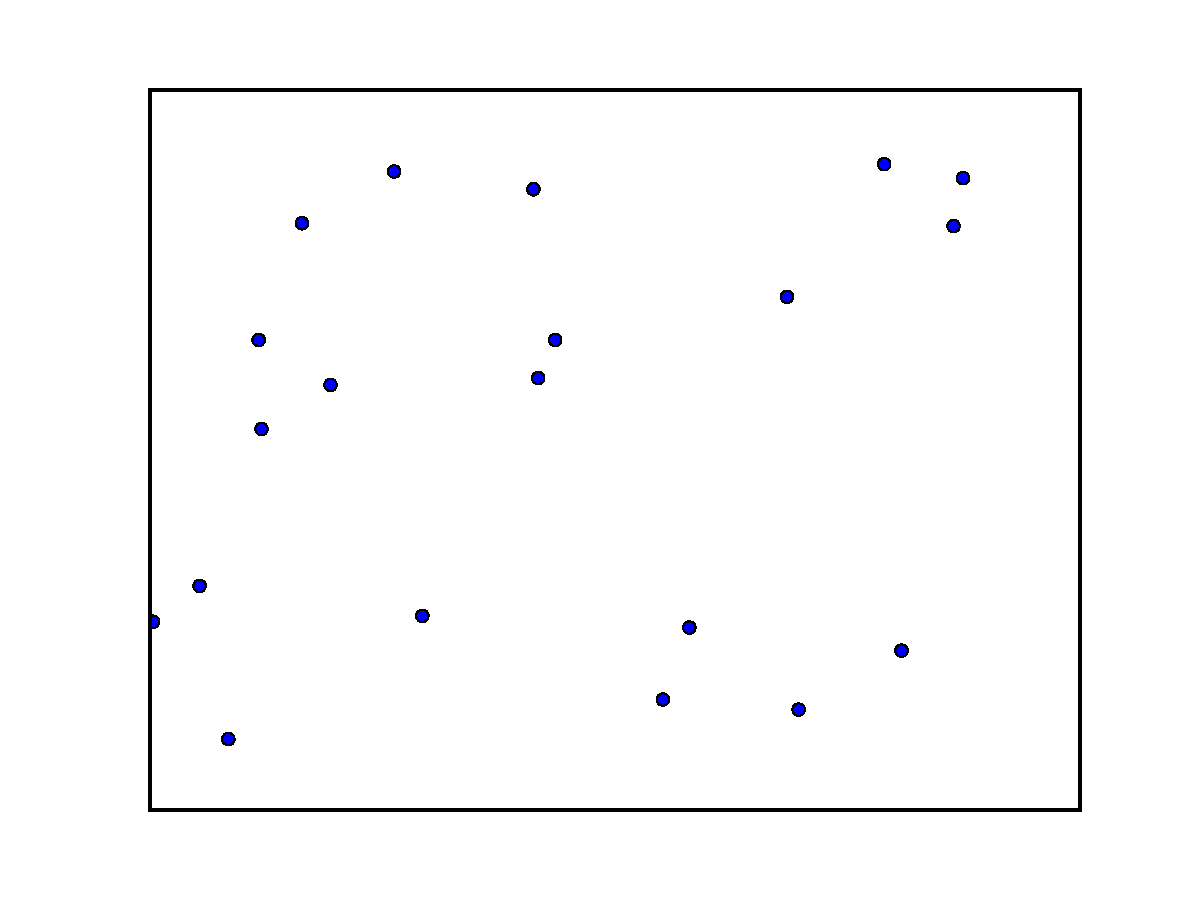
\includegraphics[width=0.4\textwidth]{chapter_ndinterp/plots/qhull_1.pdf}%
   \hfill
   \label{fig:qhull_1}%
 }\quad%
 \subfloat[We find the points with the lowest and highest x-value and connect them with a line.]{
%   \missingfigure[figwidth=0.4\textwidth]{Test}%
   \includegraphics[width=0.4\textwidth]{chapter_ndinterp/plots/qhull_2.pdf}%
   \label{fig:qhull_2}%
 }\\%
 \subfloat[Continuing with the points on the left (same process happens recursively on the right) we find the point furthest away from the line. We then draw two more lines and build a triangle. The points inside of the triangle are not part of the convex hull and are discarded. We will repeat the current step with the two new lines of the triangle. ]{%
 %  \missingfigure[figwidth=0.4\textwidth]{Test}%
   \includegraphics[width=0.4\textwidth]{chapter_ndinterp/plots/qhull_3.pdf}%
   \label{fig:qhull_3}%
 }\qquad%
 \subfloat[We have found points of the convex hull once we can't build a new triangle anymore.]{%
%   \missingfigure[figwidth=0.4\textwidth]{Test}%
   \includegraphics[width=0.4\textwidth]{chapter_ndinterp/plots/qhull_final.pdf}%
   \label{fig:qhull_4}%
 }\quad%
   \caption{Determination of a convex hull in two dimensions. }%
   \label{fig:example}%
\end{figure}%

As an initial input we have N data points. Although this method works in n-dimensions, we will show an example in two dimensions.
The first operation is finding the two extreme points in the horizontal axis, which are guaranteed to be part of the convex hull. 
We connect these two extreme points thus creating a division between a ``left'' and a ``right'' set of point. Now the divide and conquer method begins. We will only describe what happens to the left side, but imply that the same steps are taken on the right side. 
We find the point furthest away from the dividing line and add it. A triangle is formed out of the two points of the initial dividing line and the additional point. All points inside the triangle do not belong to the convex hull and thus we exclude them. The triangle again divides the remaining points into two sets, one left of the triangle and one right which are again iterated over recursively. 

The method is repeated until each subset only contains the start and end point of the dividing line. 
We have created the convex hull, which if projected to a $d - 1$-dimensional space provides the \deltri\ of the projected points. For this projection to work we need to construct a convex hull in more than two dimensions which uses the same technique as described.


\section{Barycentric coordinates system}

The actual interpolation transforms the interpolant's coordinate into the barycentric coordinates of the containing triangle.

One can construct the barycenter of a triangle by drawing lines from each point to the midpoint of the opposing side (see Figure \ref{fig:tri_barycenter}). 


\begin{figure}[htbp] %  figure placement: here, top, bottom, or page
   \centering
   \includegraphics[width=0.7\textwidth]{chapter_ndinterp/plots/barycenter.pdf}
   \caption{The triangle and its barycenter marked by the intersection of lines. }
   \label{fig:tri_barycenter}
\end{figure}


The coordinates of the barycenter M can simply be expressed by,
\[
\vec{M} = \frac{1}{3} (\vec{A} + \vec{B} + \vec{C}).
\]

Not only the barycenter can be expressed by the vectors of $\vec{A}$, $\vec{B}$ and $\vec{C}$ but every point p inside the triangle can be expressed by,
\[
\vec{p} = \alpha\vec{A} + \beta\vec{B} + \gamma\vec{C},
\]
where
\[
\alpha + \beta + \gamma = 1.
\]
$\alpha$, $\beta$ and $\gamma$ are called the barycentric coordinates. If the point p lies within the triangle all barycentric coordinates are positive. 

\section{Triangle Finding and Interpolation}

To calculate the interpolation using barycentric coordinates we need to find the n-simplex that contains the interpolant. We use a method called directed walk (priv. comm. Pauli Virtanen).  We choose a random starting n-simplex. In order to interpolate to a given point (interpolant) we calculate the barycentric coordinates for the interpolant and test if all of them are larger than 0. In that case  we have found the n-simplex that contains the point. 
If the n-th barycentric coordinate is negative we jump to the neighbouring n-simplex which is opposite the n-th point. This is iterated until the containing n-simplex is found or the next jump would lead outside the convex hull of the \deltri. For the latter case the point is outside of the grid and can not be interpolated.

If this algorithm converges and the right n-simplex is found the interpolation can be easily performed using the barycentric coordinates:
\[
f(\vec{p})=\alpha f(\vec{A}) + \beta f(\vec{B}) + \gamma f(\vec{C})
\]
where  $\vec{A}$, $\vec{B}$ and $\vec{C}$ are the points of the triangle. 


\section{Conclusion}

We have described the method of linear interpolation using \deltri\ mainly in two dimensions. As mentioned this method is easily extensible to n dimensions. The triangles (3-simplices) become n-simplices in n dimensions (e.g. Tetrahedrons in three dimensions). The method itself however stays very similar for higher dimensions. 

In this work we have made extensive use of n-dimensional linear interpolation using the implementation present in the \gls{scipy} package, called \textsc{LinearNDInterpolator}. In this case creation of the convex-hull is performed by the QHULL implementation described in \citet{Barber96thequickhull}.

We have tested the performance of the algorithm by creating a three dimensional grid with $20\times10\times10$ gridpoints and an array of 10, 000  double values at each gridpoint. 
On a standard 2011 MacBook Pro (Intel Core i7, 2.6 GHz, running only on a single processor) we have measured the initial building of the \deltri and storing it in an appropriate data structure to 256\,ms. The interpolation for random points took on average $\approx600\,\mu$\,s. This technique lends itself very well to explore large datasets even on moderately equipped machines. 

We have used this technique extensively to interpolate a spectral grid in three dimension (\gls{teff}, \gls{logg}\ and \gls{feh}). When trying to extract stellar parameters from an input spectrum we calculated the $\chi^2$ for the observed spectrum with interpolated synthetic spectra from the grid. The interpolated spectra resulting from the interpolation are continuous, but not differentiable at the ridges of the grid structure (ridges are the borders of the simplices that make the grid). This non-differentiability at the ridges can be seen even in the $\chi^2$ space. Optimisers that employ gradient methods \citep[such as MIGRAD][]{James:1975dr} show some difficulties in some regions of the search space. We have tried to alleviate this problem by beginning the optimisation from different starting points. In almost all cases this lead to the same minimum.

In summary, the presented linear n-dimensional interpolator is a very robust and quick way to explore large parameter spaces without having to compute each single point. 

Future work will be directed to exploring other n-dimensional interpolators in the astrophysical context. 


% !TEX root = ../thesis.tex
\chapter{Genetic Algorithms}
\label{chap:ga}
\section{Introduction}
Numerical mathematics has been developing steadily over the last century and especially over the last 50 years when computers became readily available.  Like many other sciences numerical mathematics has been getting much inspiration from nature.  Advancements in our understanding of the brain inspired numerical mathematicians to recreate some of the structures of this biological computer. These attempts resulted in Neural Networks which today have wide applications in many areas of science and engineering. Optimisation algorithms, which are a sizeable subfield of numerical mathematics, have also borrowed heavily from nature. Some examples are Ant Colony Optimisation and Particle Swarm Optimisation. The time line in Figure \ref{fig:timeline} shows some of the milestones in optimisation.

\begin{figure}[tb]
\begin{chronology}[5]{1965}{2000}{2.5ex}{\textwidth}
\event{1965}{Amoeba(Simplex) optimisation; Evolution strategies}
%\event{1966}{Evolutionary programming}
\event{1975}{Genetic Algorithms}
\event{1983}{Simulated Annealing}
\event{1992}{Ant Colony Optimization}
\event{1993}{multiobjective Genetic Algorithms}
\event{1995}{Particle Swarm Optimization; \glsentryname{nfl}}
\event{1997}{Differential Evolution}
\end{chronology}

\caption{Time line of milestones in numerical optimisation}
\label{fig:timeline}
\end{figure}

Biological evolution can be seen as an optimisation algorithm that adjusts organisms to adapt well to their environment.  The idea of an algorithm which imitates the principal of natural evolution was first introduced by \citet{Holland:1962:OLT:321127.321128}. Shortly after other groups independently started using similar approaches \citep[e.g.][]{Rechenberg1973}. The entire field of evolutionary algorithms has since split up into many subfields (e.g. genetic programming, evolutionary programming, evolution strategy, evolutionary algorithms, etc.). Out of these subfields, the \glspl{ga} are the most widely known and have been applied to many different problems. 

In general, optimisation algorithms have two seemingly conflicting goals: exploiting good leads (optimum seeking) while still exploring the parameter space sufficiently. Simple algorithms like Hillclimbing (randomly selecting a point in the neighbourhood of the current point and then picking the better point as the new basis) will exploit good leads but will neglect to explore the search space often leading to the convergence on local optima. Random searches, on the other hand, are excellent at exploring the search space but will fail to quickly converge on an optimal solution (and are not guaranteed to converge at all). Which algorithm to use naturally depends on the type of parameter space. Spaces with independent variables can be solved relatively simply by employing optimum seeking methods. Random search algorithms are suited to parameter spaces with highly correlated variables. One should note that the better an algorithm is optimised for a specific search space the more poorly it performs on other problems. This constitutes the so called  \gls{nfl} , which also states that across the space of all problems, all algorithms perform equally well. \glspl{ga} seem to strike a balance between exploration and exploiting the current best solution. Consequently they can be applied to a wide range of different parameter spaces. In addition, they have many options and fine tuning parameters so that one can adjust them to individual problems. 

\section{Genetic Algorithms}
\glspl{ga} are a stochastic search technique that tries to find solutions in n-dimensional search spaces. In most optimisation algorithm we have a function $f(\vec{x})=s$, where $\vec{x}$ is are the input parameters and $s$ is a solution scalar (sometimes referred to as figure-of-merit). The goal is to find the input parameters that optimise $s$ (finding a maximum or minimal value of $s$). In some optimisation algorithms, however,  this function $f(\vec{x})$ does not immediately produce a scalar solution $s$ but instead produces a solution vector $\vec{y}$ (e.g. curve fitting where input coefficients produce a number of output points). This gives two option, first we can find a function $g(\vec{y})=s$ that maps the solution to an optimisable scalar and proceed as above, or we can try to optimise the individual components of $\vec{y}$ simultaneously. The latter option is called multi-objective optimisation and is a vast field of research, but outside the scope of this work. From now on we will consider that we have a function $f(\vec{x})=\vec{y}$ and a function $g(\vec{y})=s$. 

\glspl{ga} have terms for the described functions and parameters that borrow heavily from evolutionary science. The individual input parameters of $\vec{x}$ are often referred to as \glspl{gene}. The input vector $\vec{x}$ is called \gls{individual} or sometimes \gls{genome}. We refer to representation in parameter space as \gls{genotype} ($\vec{x}$) and the representation in solution space as  \gls{phenotype} ($\vec{y}$) of a solution. This is similar to biology where the input $\vec{x}$ can be thought of as the DNA sequence. The \gls{phenotype} in biology however does not resemble a vector (strictly speaking).  Mathematically speaking it is possible to have multiple \glspl{genotype} map to one \gls{phenotype}, however each \gls{genotype} only maps to one phenotype. 
One should also note that in many, if not most, optimisation problems there exists no \gls{phenotype} as the function $f(\vec{x})$ maps directly to the optimisable scalar $s$. Finally, the function that results in the figure-of-merit ($f(\vec{x})=s$ or $g(\vec{y})=s$) is called the \gls{fitness} function which results in the \gls{fitness} $s$. 

In general, \glspl{ga} maintain a pool of \glspl{individual} called a population or generation. The general idea is that each new generation is created out the old generation. Owing to the special processes of the \gls{ga} each new generation will consist of \glspl{individual} that are on average closer to the optimal solution than the last generation. Following the notation of \citet{Michalewicz:1994:GAD:184675} we introduce the population $P(t)$ with the \glspl{individual}  $\{p_{1}^{t}, \dots, p_{n}^{t}\}$, where $t$ denotes the iteration (or generation number). Each individual $(p_{i}^t)$ is a data structure consisting of a vector $\vec{x}_i$ and its corresponding fitness scalar $s_i$.  When we speak of evaluating $p_{i}^{t}$ we mean that we use $g(f(\vec{x}_i))=s_i$ to determine the fitness. A new population (or generation) $P(t+1)$ is formed by choosing, in the \textit{select step}, the more fit individuals. Some or all of the new population undergo transformations in the \textit{recombine step}. These transformations are called genetic operators. We define unary transformations, which create new individuals by small changes in single individuals called \glspl{mutation}. Higher order transformations called \glspl{crossover} combine the traits of multiple individuals to form a next generation individual. 
After the new population has been created in the \textit{recombine step}, it is evaluated (perform the computation $g(f(\vec{x}_i))=s_i$) and the \textit{select step} begins anew. 

This procedure is repeated until some termination condition is reached (see Algorithm \ref{alg:evol_program}). One way is to wait until best individual in a generation or the whole generation has reached a certain threshold fitness.  Another way is to set a limit on the number of generations. 



\begin{pseudocode}{Genetic Algorithm}{ }
\label{alg:evol_program}
\PROCEDURE{Genetic Algorithm}{}
t \GETS 0 \\
\CALL{Initialize}{P(t)}\\
\CALL{Evaluate}{P(t)}\\
\WHILE (\textrm{\textbf{not} termination condition}) \DO
\BEGIN
t \gets t+1\\
P(t) \GETS \CALL{Select}{P(t-1)}\\
\CALL{Recombine}{P(t)}\\
\CALL{Evaluate}{P(t)}\\
\END
\ENDMAIN
\end{pseudocode}



In order to apply a \gls{ga} to an optimisation problem, the following are needed:
\begin{itemize}
\item a genetic representation of the search space (e.g. a vector)
\item a function (or a chain of functions) that can calculate a fitness for a genetic representation
\item transformations that create a new population/generation out of selected members of the old population/generation
\item a method of creating an initial population
\end{itemize}


All of these points need to be considered before developing a \gls{ga} for any given problem. This involves multiple steps the first of which is choosing a suitable genetic representation for each solution in the parameter space. 

There are two main ways to represent a \gls{genome}, binary encoding and value encoding (sometimes called gray encoding). Binary encoding was the form of encoding  used in early genetic algorithms, the advantage being that the same \gls{ga} can be easily adapted for many problems. In one-dimensional problems, for example, value encoding only offers one gene, whereas binary encoding, depending on the requested precision of the value, offers multiple genes. This becomes obvious in the one-dimensional minimization example: $f(\vec{x})=(x_0 - 3.141)^2$. The solution vector that minimises the problem in value encoding is $\vec{x} = (3.141)$ using IEEE 754 floating point encoding the optimal vector is $\vec{x}=(0,1,0,0,0,0,0,0,0,1,0,0,1,0,0,1,0,0,0,0,0,1,1,0,0,0,1,0,0,1,0,1)$.
There are however many problems with binary encoding. The so called \textit{hamming cliff} describes the problem that a simple bit-flip at one high encoding bit (occurring in the \textit{recombination step} using \gls{mutation} or \gls{crossover}) can dramatically change the encoded value \citep[e.g.][]{Chakraborty2003253}. This can improve covering of search space but also can hinder the code from converging. In addition, when using binary encoding for many input variables the genomes can get incredibly long and \glspl{ga} have been shown to perform poorly for very long genomes. Value encoding often is a natural way to encode the parameters of a problem. In contrast to binary encoding the genetic operators are often much more problem specific. It seems that for the moment value encoding is the preferred method in many cases \citep[e.g.][]{Janikow1991Comparison,Wright91geneticalgorithms,Goldberg90real-codedgenetic}. The \gls{nfl} theorem proves that there is no one optimal encoding, but the optimal encoding is different for each problem.

The fitness function maps the phenotype ($\vec{y}$) to a scalar and is one of the requirements for optimisation. It is often hard to define one number that describes how good a solution is for any given problem. For example it is not possible to map desirable traits of a car to one number and one might have prioritize which traits to optimise at the cost of others. A sensible \gls{fitness} function that maps from the multi-dimensional \gls{phenotype} to a scalar is sometimes impossible to construct. As described above these cases need to be treated under multi-objective optimisation schemes. Multi-objective optimisation is a vast field of research and outside the scope of this work. 

Many \glspl{ga} employ a so called \gls{fitness} scaling operation in every generation to the \gls{fitness} function. This scaling often helps the \gls{ga} to follow promising leads but also explore the parameter space. For example, it sometimes happens, especially in early generations, that a \gls{fitness} function values a small fraction of individuals extremely highly when compared to the rest of the solutions. These \glspl{individual} with a near optimal value in very few \glspl{gene} might have a much higher \gls{fitness} than an \gls{individual} with a subpar value for these few \glspl{gene}, but which has near optimal values for all other \glspl{gene}. The subsequent populations will then be reigned by the \glspl{gene} of these few individuals which prohibits the \gls{ga} from exploring the search space. In \gls{ga} terms individuals with extremely high fitness based on very few near optimal \glspl{gene} are called \glspl{superindividual}. They can drastically reduce the genetic breadth and often cause the \gls{ga} to fail. One way to overcome this problem is scaling the fitness of all individuals after they have been computed. There are other steps which can be undertaken in the \textit{select step} described later. The scaling is often a simple algebraic transformation, like linear or exponential scaling. A specific example can be found in Section \ref{sec:dalek}. In addition to fitness scaling, there exists the possibility to just use the rank of the individuals as a \gls{fitness} measure. In the case of ranking, we order the \glspl{individual} according to their \gls{fitness} value and assign them monotonically incrementing values (see Figure \ref{fig:rankselection}). In summary, fitness functions and scaling are a very crucial part of a successful algorithm. For a description of different scaling methods please refer to \citet{Kreinovich93geneticalgorithms}.

\Glspl{superindividual} can not only be avoided with \gls{fitness} scaling but also by initial population choice. The most basic quantity to consider when choosing the initial population is that of population size. Generally the population size remains the same over the course of a \gls{ga}. The population size should be chosen in relation to the size and complexity of the parameter space. For example, a small population size and a large search space can lead the \gls{ga} to find local optima rather than the global optimum. In this work, we have chosen a population which is roughly 15 times bigger than the number of input parameters. After having chosen the population size the most basic method of selecting the initial population is to draw individuals uniformly and randomly from the entire search space. One might however know a probability distribution for the parameter space and can draw randomly weighted by the distribution (e.g. when trying to find find parameters for a random star, we can rule out a 20\,\msun white dwarfs with some likelihood). An initial population that is closer to predicted optimal values will converge faster, but won't explore the parameter space that well. 

Once we have evaluated the fitness for each member of the \gls{individual} population the next step is the \textit{selection step}. There are many different approaches for selecting \glspl{individual} from the current generation to create the next generation. Before selecting \glspl{individual} we can a make coarse selection on the entire population. One selection that is often performed is \gls{elitism} in which a fraction of the fittest individuals is selected to advance unaltered to the next generation. Another possibility is to discard a fraction of the least fit \glspl{individual}. The \gls{gene} combinations of these  \glspl{individual} then won't be used in the upcoming \textit{recombination step}. After this first coarse selection on the population the remaining members form the so-called mating population.

We then start with the recombination step acting only on the current mating population. The first action in the recombination step is the selection of two or more individuals from the mating population and subsequent addition to a mating pool. A mating pool is a collection of \glspl{individual} whose \glspl{gene} will be combined to form one or more \glspl{individual} of the next generation. In all our next examples we will assume a mating-pool with only two slots (similar to two parents in biological reproduction). There is a multitude of options for selecting members from the mating population and adding them to a mating pool \citep[for an overview see][]{Goldberg91acomparative}. The most widely used of the selection algorithms is the \gls{rws}. In Figure \ref{fig:roulettewheel} we see that \glspl{individual} are assigned a wedge of the wheel. The area of the wedge is according to the \gls{individual}'s fitness. The wheel is then spun and slows down until the wheel comes to a halt. The selection chevron on the left points then to the chosen \gls{individual}. In \gls{rws} fitter \glspl{individual} are more likely to be chosen than \glspl{individual} with poorer \gls{fitness}. In Figure \ref{fig:rankselection} we show how rank scaling of the fitnesses can alleviate the problem of early \glspl{superindividual}. In addition to \gls{rws} there is \textit{tournament selection} where we randomly select two individuals and compare those. The fitter of those two individuals is selected. 

\begin{figure}[tb] %  figure placement: here, top, bottom, or page
   \centering
   \includegraphics[width=\textwidth]{chapter_ga/plots/rws_cropped.pdf} 
   \caption[Roulette Wheel Selection]{The individual fitnesses are assigned proportional fractions on the roulette wheel. The wheel is then spun and will slowly decelerate and stop at some point. Individuals with a higher fitness have a higher chance of being chosen with this method.}
   \label{fig:roulettewheel}
\end{figure}

\begin{figure}[tb] %  figure placement: here, top, bottom, or page
   \centering
   \includegraphics[width=\textwidth]{chapter_ga/plots/rank_select.pdf} 
   \caption[Rank Selection with subsequent Roulette Wheel Selection]{We assign new fitness values to individuals before assigning them probabilities on the roulette wheel. The fitnesses are assigned by location in an ordered list. The least fit individual gets assigned the value 1 the fittest individual the number n, where n is the population size. This is can be viewed as a special case of fitness scaling. After the new fitnesses have been chosen we use normal roulette wheel selection to select for the mating pool in the population. }
   \label{fig:rankselection}
\end{figure}

There are multiple steps for creating a new population from the current mating population. In the previous paragraph we described how to select \glspl{individual} and place them in a mating pool. The \glspl{individual} in the mating pool are also often referred to as \glspl{parent}. Similar to the term \gls{parent} we refer to the newly created \glspl{individual} as \glspl{child}. The reader should notice that the same individual can be in the mating pool twice (unlike with biological \glspl{parent})! We create one or multiple \glspl{child} from this mating pool and place them in the next generation. The current mating pool is disbanded and a new one is formed. These steps are repeated until the new population has the same number as the old population (minus the number of individuals that advanced to the new population through \gls{elitism}). There are two main processes to create a new individual from a mating pool: \gls{crossover} and \gls{mutation}. The simplest form of a \gls{crossover} is the single-point \gls{crossover} (see Figure \ref{fig:crossover}). A random integer $r \in [1,N-1]$, where N describes the number of \glspl{gene} in a \gls{genome}, is selected. The new individual is created out of the first $r$ genes from the first parent and the last $N-r$ genes from the second parent (see Figure \ref{fig:crossover}). Now it is trivial to create a second child (using the same random number $r$) from the mating pool by just switching first and second \gls{parent}. 
Two-point \gls{crossover} is very similar to single-point crossover. In two-point \gls{crossover} Two random numbers are selected and the crossover occurs at these places. Multi-point \gls{crossover} (see Figure \ref{fig:crossover}) is essentially just an extension of two-point \gls{crossover}. In addition, there is uniform \gls{crossover} in the case that each gene is selected randomly with equal chance from either parent. Finally, arithmetic \glspl{crossover} use a function to calculate the new gene from each of the parent genes. For a value encoding this function could be the \emph{mean} function. For a binary encoding the function could be the \textit{and} operator. 
One can mix arithmetic and Multi-point  crossovers. For example we select the $r$ genes from the first parent and create the last $N-r$ genes by taking the mean of first and second parent's \glspl{gene}. After the new child or children have been created through \glspl{crossover} they are subjected to the mutation operator. There is a chance for each individual gene (often chosen to be less than 5\%) that it is altered. For bit encoding this altering is a simple bit inversion. There are many options for value encoding. For example, one can add or multiply with a random number. Once this step is complete the children are added to the new population.

\begin{figure}[tb] %  figure placement: here, top, bottom, or page
   \centering
   \includegraphics[width=\textwidth,trim=0 18cm 0 0]{chapter_ga/plots/crossovers.pdf} 
   \caption[Single-point and multi-point crossover]{In the single-point crossover a random point in the \glsentryname{individual} is chosen. Before this point the genes are taken from the first parent and after that the we use the genes from the second parent. Using the same random number it easily allows for the creation of two children by reversing the roles of first and second parent. The multi-point crossover employs multiple places in the genome where the crossover happens.}
   \label{fig:crossover}
\end{figure}

Once the new generation is created by \glspl{crossover} and \glspl{mutation} we start the iterative process anew. First we calculate the \gls{fitness} of all \glspl{individual}, then scale the resulting \gls{fitness}, create a mating population and select \glspl{individual} with, for example, \gls{rws}  to create children which forms the next generation. This iterative process is run until we have reached a certain number of generations or some \glspl{individual} have reached some \gls{fitness} threshold. 

\section{Convergence in Genetic Algorithms}
A key problem with many \gls{ga}-implementations is the premature convergence on a local optimum. The more complex the search space and the more interlinked the parameters are, the more likely it is that traditional search routines will fail. \glspl{ga} are inherently better at bypassing local optima but are in no way immune to this problem. A feature that separates \glspl{ga} from traditional optimisation algorithms is that they will never fully converge. The algorithm will get close to the optimum but due to continued mutation of the individuals the \gls{ga} will in most cases not reach an optimal value. To alleviate this problem some authors suggest switching to a different algorithm when close to the optimal solution, whereas others suggest changing the mutation rate over time \citep[see][and references therein]{citeulike:344183}.

One of the unsolved problems is determining a mathematical description for the \glspl{ga} convergence. The next section is dedicated to the predominate schemata theory, which however only explains a subset of the intrinsic complexity of \glspl{ga}.

\section{Genetic Algorithm Theory}

The schemata theory first described by \cite{holland1975} is one of the accepted theoretical interpretations of \glspl{ga}. There is some criticism and it is known that this theory only explains part of the complexity that are inherent to \glspl{ga} \citep[see ][ and references therein]{Whitley94agenetic}. We will describe the basic concepts of schemata using an example in binary encoding \citep[notation adapted from ][]{citeulike:125978}. A schemata or similarity template is formed by adding an extra letter to the binary alphabet denoted by $*$. Using the ternary alphabet ${0, 1, *}$ we can now describe a pattern matching schemata were the $*$ symbol can be thought of as \textit{don't care}-symbol. The schemata ${0, 1, 0, *}$ for example, matches both the string ${0, 1, 0, 0}$ and ${0, 1, 0, 1}$. The order of a schemata is defined as how many places are not filled by the $*$-symbol. For example, the given example is a third order schemata. Schematas provide a powerful way to describe similarities in a set of \glspl{individual}. 
A whole population with many \glspl{individual} therefore samples a range of different schematas . Essentially low-order and above-average schemata receive exponentially increasing trials in subsequent generations of a \gls{ga}. \citet{Michalewicz:1994:GAD:184675} describe the workings of a \gls{ga} in the following way: ``A genetic algorithm seeks near optimal performance through the juxtaposition of low-order, high-performance schemata, called building blocks''.
This schemata theory is the standard explanation for \glspl{ga}, there are however some examples that violate the implications that stem from this schemata theory \citep[see Chapter 3 of][for some examples]{Michalewicz:1994:GAD:184675}.

\section{A Simple Example}

As a last explanation we will offer a simple example, to give a more `hands-on' description of \glspl{ga}.We will illustrate the use of a \gls{ga} on a simple astrophysical problem. The task at hand is to fit an observed spectrum with a synthetic spectrum. The input parameters for this synthetic spectrum are \gls{teff}, \gls{logg}, \gls{feh}, $\alpha$-enhancement, \vrad\ and \vrot. The simplest genetic representation of this is the vector $\vec{x} = (\teff, \logg, \feh, \alpha, \vrad, \vrot)$. $\vec{x}$ is the \textit{genotype} of the individual. The resulting synthetic spectrum is the \textit{phenotype}. 

For this relatively small number of genes a population size of 75 should suffice. The first step is drawing an initial population. We will draw uniformly randomly from the search space: $\teff \in [2000, 9000]$, $\logg \in [0, 5]$, $\feh \in [-5,1]$, $\alpha \in [0,0.4]$, $\vrad \in [-100, 100]$ and $\vrot \in [0,200]$. We compute the synthetic spectrum for each individual. The fitness of each individual is the inverse of the root-mean-square of the residuals between the observed and the synthetic spectrum. 
In the select step we will first advance 10 \% of the fittest individuals to the next population unaltered (\gls{elitism}). For the next population to be complete we need $75 - 8 = 67$ individuals which are created through mating. We select two individuals through \gls{rws} and place them in the mating pool. A single crossover point is randomly selected and the child is created. Before being placed in the new population the mutation operator is applied but has a very small chance to mutate any of the child's genes (in this case we choose 2\%).
This mating step is repeated 67 times. The new population now consists of the 8 fittest individuals of the old population and 67 new individuals created by mating. We will then start again to compute the synthetic spectrum and the resulting fitness for each individual of the new population. This loop is continued until one individual or a whole population has reached a predefined convergence criterium.

\section{Conclusion}

\glspl{ga} with their inherently parallel nature are very useful in the increasingly parallel computing. They are relatively easy to implement and can be used for a variety of problems. In many applications \gls{ga} quickly deliver impressive results, but require a lot of time for fine-tuning to be able to sufficiently handle the problem. \glspl{ga} also offer a plethora for each of the individual steps (encoding type, selection type, etc.), which can confuse users that are not very familiar with the consequence for each choice. To alleviate this problem in our work we have sought the help of experts in \glspl{ga} and hope to find the best set of options for our \gls{ga}. 
In summary, although there are some drawbacks (no guaranteed convergence, many choices for implementation, etc.) we find that we progressed much quicker with \glspl{ga} than with other algorithms. 



\chapter{SN 1006 Data}
% !TEX root = ../single_chapter_sn1006.tex
\ctable[
pos=p,
%width=\textwidth,
doinside=\scriptsize,
caption=SN1006 photometry,
label=tab:sn1006_photometry]
{lccccccccccc}{}{\FL
Name & RA & Dec & $\theta$ & U & $\sigma_\textrm{U}$ & B & $\sigma_\textrm{B}$ & V & $\sigma_\textrm{V}$ & I & $\sigma_\textrm{I}$\\ 
 & hh:mm:ss & dd:mm:ss & $\arcsec$ & mag & mag & mag & mag & mag & mag & mag & mag\ML
 SN1006 01 & 15:02:58.27 & -41:55:20.9 & 67.8 & 16.03 & 0.02 & 14.76 & 0.00 & 13.50 & 0.08 & 12.30 & 0.18\\
SN1006 02 & 15:02:59.95 & -41:56:25.2 & 86.1 & 18.84 & 0.08 & 16.96 & 0.01 & 15.37 & 0.01 & 13.95 & 0.05\\
SN1006 03 & 15:02:51.80 & -41:56:39.9 & 49.8 & 16.16 & 0.02 & 15.86 & 0.01 & 15.04 & 0.01 & 14.23 & 0.09\\
SN1006 04 & 15:02:53.35 & -41:54:18.0 & 93.6 & 16.67 & 0.02 & 16.33 & 0.00 & 15.47 & 0.00 & 14.62 & 0.00\\
SN1006 05 & 15:02:49.97 & -41:56:23.9 & 45.7 & 16.90 & 0.03 & 16.41 & 0.00 & 15.50 & 0.01 & 14.65 & 0.00\\
SN1006 06 & 15:02:45.68 & -41:54:35.2 & 110.5 & 16.21 & 0.01 & 16.17 & 0.01 & 15.50 & 0.00 & 14.78 & 0.01\\
SN1006 07 & 15:02:51.19 & -41:55:58.5 & 19.8 & 17.62 & 0.05 & 16.91 & 0.02 & 15.90 & 0.01 & 14.92 & 0.02\\
SN1006 08 & 15:02:47.00 & -41:55:28.3 & 69.3 & 16.57 & 0.03 & 16.53 & 0.01 & 15.86 & 0.01 & 15.16 & 0.00\\
SN1006 09 & 15:02:55.07 & -41:57:14.4 & 86.6 & 18.46 & 0.20 & 17.73 & 0.01 & 16.58 & 0.01 & 15.53 & 0.02\\
SN1006 10 & 15:03:01.87 & -41:54:59.2 & 113.4 & 17.18 & 0.04 & 17.06 & 0.00 & 16.30 & 0.00 & 15.51 & 0.00\\
SN1006 11 & 15:02:56.05 & -41:54:53.5 & 68.1 & 17.02 & 0.03 & 17.12 & 0.00 & 16.33 & 0.05 & 15.61 & 0.01\\
SN1006 12 & 15:02:58.83 & -41:56:35.5 & 80.0 & 17.60 & 0.03 & 17.22 & 0.00 & 16.39 & 0.02 & 15.50 & 0.02\\
SN1006 13 & 15:02:49.22 & -41:57:31.1 & 107.6 & 17.93 & 0.09 & 17.41 & 0.01 & 16.49 & 0.00 & 15.74 & 0.06\\
SN1006 14 & 15:02:59.24 & -41:54:51.6 & 93.1 & 17.93 & 0.04 & 17.44 & 0.00 & 16.56 & 0.00 & 15.75 & 0.01\\
SN1006 15 & 15:03:00.33 & -41:56:29.8 & 91.9 & 17.81 & 0.01 & 17.42 & 0.01 & 16.63 & 0.01 & 15.87 & 0.04\\
SN1006 16 & 15:02:58.09 & -41:54:47.9 & 86.4 & 19.60 & 0.47 & 18.37 & 0.01 & 17.26 & 0.00 & 16.11 & 0.03\\
SN1006 17 & 15:03:02.49 & -41:55:46.7 & 107.7 & 17.45 & 0.02 & 17.40 & 0.00 & 16.66 & 0.04 & 16.02 & 0.13\\
SN1006 18 & 15:02:50.99 & -41:56:39.4 & 52.2 & 18.00 & 0.03 & 17.61 & 0.00 & 16.77 & 0.03 & 15.87 & 0.04\\
SN1006 19 & 15:02:50.12 & -41:57:05.5 & 80.1 & 20.28 & 0.00 & 18.75 & 0.01 & 17.39 & 0.01 & 16.01 & 0.00\\
SN1006 20 & 15:02:48.03 & -41:56:19.4 & 60.6 & - & - & 19.59 & 0.03 & 18.04 & 0.01 & 15.97 & 0.17\\
SN1006 21 & 15:02:58.44 & -41:54:50.1 & 87.5 & 20.60 & 0.00 & 18.47 & 0.01 & 17.36 & 0.01 & 16.30 & 0.03\\
SN1006 22 & 15:02:59.95 & -41:55:41.9 & 79.8 & 17.26 & 0.04 & 17.25 & 0.00 & 16.71 & 0.06 & 16.18 & 0.04\\
SN1006 23 & 15:02:43.94 & -41:56:15.4 & 102.3 & 19.62 & 0.32 & 18.50 & 0.01 & 17.39 & 0.00 & 16.24 & 0.01\\
SN1006 24 & 15:02:56.14 & -41:54:49.2 & 72.3 & - & - & 18.28 & 0.00 & 17.59 & 0.13 & 16.49 & 0.11\\
SN1006 25 & 15:02:59.79 & -41:56:43.2 & 93.1 & 17.75 & 0.01 & 17.64 & 0.06 & 17.03 & 0.02 & 16.35 & 0.03\\
SN1006 26 & 15:02:54.92 & -41:55:27.7 & 33.1 & 18.10 & 0.10 & 17.95 & 0.01 & 17.23 & 0.02 & 16.43 & 0.00\\
SN1006 27 & 15:02:52.72 & -41:55:58.9 & 7.6 & 18.61 & 0.08 & 18.26 & 0.02 & 17.47 & 0.03 & 16.64 & 0.05\\
SN1006 28 & 15:02:54.86 & -41:56:36.4 & 50.2 & 18.52 & 0.13 & 18.24 & 0.00 & 17.43 & 0.02 & 16.70 & 0.02\\
SN1006 29 & 15:02:51.84 & -41:54:47.9 & 64.5 & - & - & 19.23 & 0.00 & 18.00 & 0.02 & 16.72 & 0.04\\
SN1006 30 & 15:02:44.71 & -41:55:15.4 & 97.7 & 18.05 & 0.03 & 18.24 & 0.03 & 17.54 & 0.02 & 16.75 & 0.01\\
SN1006 32 & 15:02:53.61 & -41:55:13.7 & 38.7 & 18.72 & 0.18 & 18.42 & 0.02 & 17.64 & 0.03 & 16.78 & 0.03\\
SN1006 33 & 15:02:43.38 & -41:55:51.5 & 105.7 & 19.07 & 0.23 & 18.56 & 0.04 & 17.66 & 0.04 & 16.69 & 0.05\\
SN1006 34 & 15:02:56.13 & -41:56:05.1 & 39.1 & 18.64 & 0.11 & 18.52 & 0.02 & 17.76 & 0.01 & 16.94 & 0.01\\
SN1006 35 & 15:02:44.66 & -41:55:10.0 & 100.4 & 19.06 & 0.17 & 18.74 & 0.00 & 17.84 & 0.02 & 16.88 & 0.05\\
SN1006 36 & 15:02:58.70 & -41:55:02.9 & 81.4 & 19.46 & 0.40 & 18.65 & 0.01 & 17.79 & 0.01 & 16.86 & 0.02\\
SN1006 37 & 15:02:58.96 & -41:55:02.5 & 83.9 & - & - & - & - & - & - & - & -\\
SN1006 38 & 15:02:50.29 & -41:55:45.6 & 29.2 & 18.58 & 0.08 & 18.48 & 0.03 & 17.80 & 0.03 & 17.00 & 0.01\\
SN1006 39 & 15:02:43.76 & -41:55:25.6 & 104.7 & 18.86 & 0.06 & 18.44 & 0.02 & 17.69 & 0.01 & 16.97 & 0.01\\
SN1006 40 & 15:02:52.23 & -41:56:37.9 & 47.0 & - & - & - & - & - & - & 16.28 & 0.06\\
SN1006 41 & 15:02:52.06 & -41:55:05.2 & 47.1 & 17.97 & 0.01 & 18.02 & 0.00 & 17.61 & 0.01 & 17.11 & 0.02\\
SN1006 42 & 15:02:57.08 & -41:54:34.3 & 90.4 & 19.22 & 0.27 & 18.78 & 0.03 & 17.99 & 0.01 & 17.16 & 0.03\\
SN1006 43 & 15:02:48.27 & -41:56:15.9 & 56.7 & - & - & 20.14 & 0.04 & 18.76 & 0.08 & 17.25 & 0.06\\
SN1006 44 & 15:02:51.96 & -41:54:31.4 & 80.7 & - & - & 19.79 & 0.01 & 18.54 & 0.02 & 17.06 & 0.01\\
SN1006 45 & 15:02:47.43 & -41:56:05.3 & 62.0 & 18.45 & 0.11 & 18.43 & 0.02 & 17.71 & 0.03 & 17.00 & 0.05\\
SN1006 46 & 15:02:49.93 & -41:57:35.3 & 108.8 & 20.09 & 0.17 & 19.04 & 0.03 & 18.05 & 0.04 & 17.19 & 0.20\\
SN1006 47 & 15:02:52.86 & -41:54:25.7 & 85.7 & 18.89 & 0.24 & 18.63 & 0.01 & 17.96 & 0.03 & 17.14 & 0.03\\
SN1006 48 & 15:02:54.52 & -41:55:29.9 & 28.5 & - & - & 19.29 & 0.03 & 18.38 & 0.01 & 17.38 & 0.06\\
SN1006 49 & 15:02:52.83 & -41:56:06.1 & 14.7 & 18.90 & 0.33 & 18.84 & 0.00 & 18.17 & 0.01 & 17.37 & 0.05\\
SN1006 50 & 15:02:53.93 & -41:56:22.6 & 33.4 & 19.68 & 0.11 & 18.99 & 0.03 & 18.07 & 0.03 & 17.19 & 0.02\\
SN1006 51 & 15:02:54.58 & -41:53:58.4 & 114.7 & 19.47 & 0.00 & 18.90 & 0.26 & 17.99 & 0.19 & 16.93 & 0.17\\
SN1006 52 & 15:03:00.97 & -41:54:58.6 & 104.9 & 19.41 & 0.17 & 18.89 & 0.00 & 18.08 & 0.03 & 17.24 & 0.02\\
SN1006 53 & 15:02:57.45 & -41:56:14.7 & 56.4 & 19.32 & 0.43 & 18.90 & 0.03 & 18.13 & 0.01 & 17.24 & 0.05\\
SN1006 54 & 15:02:48.09 & -41:57:07.7 & 92.9 & 20.33 & 0.58 & 19.40 & 0.02 & 18.45 & 0.01 & 17.48 & 0.03\\
SN1006 55 & 15:02:44.67 & -41:55:35.9 & 92.6 & - & - & 19.90 & 0.01 & 18.68 & 0.03 & 17.36 & 0.04\\
SN1006 56 & 15:02:50.38 & -41:54:34.5 & 81.7 & - & - & 20.15 & 0.16 & 18.83 & 0.06 & 17.46 & 0.08\\
SN1006 57 & 15:02:54.15 & -41:56:40.9 & 51.5 & 19.59 & 0.57 & 18.91 & 0.02 & 18.26 & 0.04 & 17.63 & 0.07\\
SN1006 58 & 15:02:49.42 & -41:55:33.5 & 42.3 & 18.90 & 0.09 & 18.92 & 0.02 & 18.21 & 0.02 & 17.41 & 0.02\\
SN1006 59 & 15:02:51.38 & -41:57:34.9 & 104.7 & 19.59 & 0.37 & 19.21 & 0.01 & 18.54 & 0.02 & 17.78 & 0.02\\
SN1006 60 & 15:02:59.64 & -41:57:03.8 & 104.8 & 20.05 & 0.18 & 19.22 & 0.01 & 18.48 & 0.13 & 18.62 & 0.43\LL}

\ctable[
%width=\textwidth,
doinside=\scriptsize,
caption=SN1006 photometry,
continued,
label=tab:sn1006_photometry]
{lccccccccccc}{}{\FL
Name & RA & Dec & $\theta$ & U & $\sigma_\textrm{U}$ & B & $\sigma_\textrm{B}$ & V & $\sigma_\textrm{V}$ & I & $\sigma_\textrm{I}$\\ 
 & hh:mm:ss & dd:mm:ss & $\arcsec$ & mag & mag & mag & mag & mag & mag & mag & mag\ML
SN1006 61 & 15:02:53.45 & -41:57:09.2 & 78.0 & - & - & 20.49 & 0.05 & 19.24 & 0.02 & 17.82 & 0.07\\
SN1006 62 & 15:02:44.94 & -41:55:48.3 & 88.3 & - & - & 19.38 & 0.02 & 18.53 & 0.01 & 17.54 & 0.01\\
SN1006 63 & 15:02:50.89 & -41:55:17.4 & 40.5 & 20.19 & 0.15 & 19.41 & 0.00 & 18.55 & 0.02 & 17.62 & 0.05\\
SN1006 64 & 15:02:55.53 & -41:57:28.3 & 101.4 & 19.45 & 0.28 & 18.87 & 0.02 & 18.51 & 0.03 & 17.87 & 0.08\\
SN1006 65 & 15:02:44.57 & -41:55:28.2 & 95.3 & 18.79 & 0.04 & 18.93 & 0.03 & 18.38 & 0.04 & 17.63 & 0.05\\
SN1006 66 & 15:02:57.28 & -41:54:19.6 & 104.3 & - & - & 20.02 & 0.03 & 19.09 & 0.02 & 18.00 & 0.03\\
SN1006 67 & 15:02:48.88 & -41:55:03.4 & 65.4 & 19.69 & 0.38 & 19.11 & 0.03 & 18.37 & 0.01 & 17.57 & 0.01\\
SN1006 68 & 15:02:43.51 & -41:56:23.9 & 109.2 & 20.65 & 0.00 & 19.60 & 0.04 & 18.75 & 0.04 & 17.94 & 0.01\\
SN1006 69 & 15:03:01.11 & -41:56:40.2 & 104.3 & 20.07 & 0.00 & 19.59 & 0.03 & 18.59 & 0.17 & 17.91 & 0.09\\
SN1006 70 & 15:02:58.01 & -41:56:45.0 & 78.6 & 20.38 & 0.57 & 19.49 & 0.01 & 18.73 & 0.03 & 18.00 & 0.06\\
SN1006 71 & 15:03:00.93 & -41:55:35.3 & 91.6 & - & - & 19.95 & 0.02 & 18.84 & 0.02 & 17.92 & 0.25\\
SN1006 72 & 15:02:58.39 & -41:57:20.6 & 108.5 & 19.34 & 0.00 & 19.90 & 0.11 & 18.85 & 0.11 & 18.01 & 0.14\\
SN1006 73 & 15:02:50.64 & -41:54:49.5 & 66.7 & - & - & 20.00 & 0.04 & 19.04 & 0.06 & 17.92 & 0.12\\
SN1006 74 & 15:03:02.32 & -41:56:05.2 & 106.6 & - & - & 19.88 & 0.08 & 18.76 & 0.16 & 18.21 & 0.02\\
SN1006 75 & 15:02:53.19 & -41:54:05.5 & 106.0 & 19.23 & 0.11 & 19.07 & 0.03 & 18.34 & 0.03 & 17.50 & 0.03\\
SN1006 76 & 15:02:44.17 & -41:55:45.8 & 97.0 & 19.56 & 0.09 & 19.40 & 0.02 & 18.70 & 0.03 & 17.91 & 0.08\\
SN1006 77 & 15:02:55.98 & -41:55:47.4 & 35.2 & 19.58 & 0.20 & 19.22 & 0.02 & 18.56 & 0.05 & 17.69 & 0.02\\
SN1006 78 & 15:02:48.76 & -41:56:59.9 & 82.3 & - & - & 20.87 & 0.10 & 19.53 & 0.01 & 18.06 & 0.05\\
SN1006 79 & 15:02:53.45 & -41:56:41.7 & 50.7 & - & - & 21.53 & 0.06 & 19.90 & 0.02 & 18.04 & 0.05\\
\LL}
\newpage
\begin{longtable}{cccccccccc}
\caption{SN 1006 infrared photometry (Candidates with $V<17.5$ marked in gray)}
\label{tab:sn1006_twomass}\\ 
\hline\multicolumn{1}{c}{Star} & \multicolumn{1}{c}{J} & \multicolumn{1}{c}{$\sigma_\textrm{J}$} & \multicolumn{1}{c}{H} & \multicolumn{1}{c}{$\sigma_\textrm{H}$} & \multicolumn{1}{c}{K} & \multicolumn{1}{c}{$\sigma_\textrm{K}$} & \multicolumn{1}{c}{QFlag} & \multicolumn{1}{c}{$T_\textrm{eff}$(B-V)} & \multicolumn{1}{c}{$T_\textrm{eff}$(V-K)}\\ 
\multicolumn{1}{c}{} & \multicolumn{1}{c}{mag} & \multicolumn{1}{c}{mag} & \multicolumn{1}{c}{mag} & \multicolumn{1}{c}{mag} & \multicolumn{1}{c}{mag} & \multicolumn{1}{c}{mag} & \multicolumn{1}{c}{} & \multicolumn{1}{c}{K} & \multicolumn{1}{c}{K}\\ \hline
\endfirsthead

\multicolumn{10}{c}{{\bfseries \tablename\ \thetable{} -- continued from previous page}} \\ \hline
\multicolumn{1}{c}{Star} & \multicolumn{1}{c}{J} & \multicolumn{1}{c}{$\sigma_\textrm{J}$} & \multicolumn{1}{c}{H} & \multicolumn{1}{c}{$\sigma_\textrm{H}$} & \multicolumn{1}{c}{K} & \multicolumn{1}{c}{$\sigma_\textrm{K}$} & \multicolumn{1}{c}{QFlag} & \multicolumn{1}{c}{$T_\textrm{eff}$(B-V)} & \multicolumn{1}{c}{$T_\textrm{eff}$(V-K)}\\ 
\multicolumn{1}{c}{} & \multicolumn{1}{c}{mag} & \multicolumn{1}{c}{mag} & \multicolumn{1}{c}{mag} & \multicolumn{1}{c}{mag} & \multicolumn{1}{c}{mag} & \multicolumn{1}{c}{mag} & \multicolumn{1}{c}{} & \multicolumn{1}{c}{K} & \multicolumn{1}{c}{K}\\ \hline
\endhead

\hline \multicolumn{10}{c}{{Continued on next page}} \\ \hline
\endfoot
\hline \hline
\endfoot
\rowcolor[gray]{0.9}  01 & 11.05 & 0.02 & 10.32 & 0.02 & 10.21 & 0.02 & AAA & 4531 & 4376\\
\rowcolor[gray]{0.9}  02 & 12.67 & 0.03 & 11.87 & 0.03 & 11.71 & 0.02 & AAA & 3990 & 4150\\
\rowcolor[gray]{0.9}  03 & 13.63 & 0.04 & 13.26 & 0.04 & 13.19 & 0.05 & AAA & 5559 & 5780\\
\rowcolor[gray]{0.9}  04 & 13.92 & 0.03 & 13.56 & 0.03 & 13.43 & 0.03 & AAA & 5467 & 5518\\
\rowcolor[gray]{0.9}  05 & 13.93 & 0.02 & 13.50 & 0.03 & 13.33 & 0.04 & AAA & 5299 & 5367\\
\rowcolor[gray]{0.9}  06 & 14.15 & 0.02 & 13.82 & 0.03 & 13.77 & 0.04 & AAA & 6051 & 5947\\
\rowcolor[gray]{0.9}  07 & 14.11 & 0.03 & 13.68 & 0.03 & 13.57 & 0.04 & AAA & 5080 & 5178\\
\rowcolor[gray]{0.9}  08 & 14.51 & 0.03 & 14.32 & 0.04 & 14.18 & 0.07 & AAA & 6067 & 6026\\
\rowcolor[gray]{0.9}  09 & 14.45 & 0.03 & 13.85 & 0.04 & 13.72 & 0.05 & AAA & 4754 & 4687\\
\rowcolor[gray]{0.9}  10 & 14.79 & 0.03 & 14.37 & 0.03 & 14.34 & 0.06 & AAA & 5751 & 5619\\
\rowcolor[gray]{0.9}  11 & 14.93 & 0.05 & 14.69 & 0.07 & 14.55 & 0.09 & AAA & 5669 & 5876\\
\rowcolor[gray]{0.9}  12 & 14.81 & 0.04 & 14.39 & 0.05 & 14.28 & 0.06 & AAA & 5523 & 5437\\
\rowcolor[gray]{0.9}  13 & 14.86 & 0.04 & 14.52 & 0.05 & 14.49 & 0.09 & AAA & 5277 & 5576\\
\rowcolor[gray]{0.9}  14 & 15.01 & 0.04 & 14.67 & 0.04 & 14.56 & 0.08 & AAA & 5420 & 5566\\
\rowcolor[gray]{0.9}  15 & 15.23 & 0.04 & 14.96 & 0.06 & 14.86 & 0.11 & AAA & 5660 & 5890\\
\rowcolor[gray]{0.9}  16 & 15.17 & 0.07 & 14.63 & 0.07 & 14.47 & 0.08 & AAA & 4843 & 4742\\
\rowcolor[gray]{0.9}  17 & 15.48 & 0.06 & 15.06 & 0.07 & 15.08 & 0.13 & AAB & 5800 & -\\
\rowcolor[gray]{0.9}  18 & 15.37 & 0.06 & 14.99 & 0.06 & 14.91 & 0.13 & AAB & 5533 & -\\
\rowcolor[gray]{0.9}  19 & 15.00 & 0.04 & 14.34 & 0.05 & 14.13 & 0.06 & AAA & 4356 & 4393\\
 20 & 14.92 & 0.04 & 14.29 & 0.05 & 14.04 & 0.07 & AAA & 4044 & 3978\\
\rowcolor[gray]{0.9}  21 & 15.41 & 0.05 & 14.96 & 0.06 & 14.90 & 0.11 & AAB & 4849 & -\\
\rowcolor[gray]{0.9}  22 & 15.70 & 0.07 & 15.43 & 0.08 & 15.06 & 0.12 & AAB & 6537 & -\\
\rowcolor[gray]{0.9}  23 & 15.35 & 0.05 & 14.76 & 0.05 & 14.51 & 0.08 & AAA & 4833 & 4673\\
 24 & 15.90 & 0.08 & 15.22 & 0.09 & 15.08 & 0.13 & AAB & 5969 & -\\
\rowcolor[gray]{0.9}  25 & 15.56 & 0.05 & 15.27 & 0.06 & 15.05 & 0.13 & AAB & 6278 & -\\
\rowcolor[gray]{0.9}  26 & 16.05 & 0.09 & 15.66 & 0.13 & 15.92 & 0.24 & ABD & 5872 & -\\
\rowcolor[gray]{0.9}  27 & 16.08 & 0.08 & 15.59 & 0.11 & 15.56 & 0.21 & ABC & 5636 & -\\
\rowcolor[gray]{0.9}  28 & 16.08 & 0.08 & 15.38 & 0.09 & 15.53 & 0.20 & AAC & 5600 & -\\
 29 & 15.75 & 0.06 & 15.18 & 0.08 & 15.09 & 0.13 & AAB & 4587 & -\\
 30 & 15.98 & 0.09 & 15.72 & 0.11 & 15.92 & 0.27 & AAD & 5932 & -\\
 32 & 16.17 & 0.11 & 15.69 & 0.12 & 15.57 & 0.19 & ABC & 5680 & -\\
 33 & 16.00 & 0.08 & 15.41 & 0.09 & 15.23 & 0.19 & AAC & 5338 & -\\
 34 & 16.25 & 0.09 & 15.54 & 0.10 & 15.62 & 0.20 & AAC & 5750 & -\\
 35 & 16.08 & 0.12 & 15.72 & 0.12 & 15.53 & 0.20 & BBC & 5346 & -\\
 36 & 16.56 & 0.13 & 16.60 & 0.24 & 15.85 & - & BDU & 5461 & -\\
 37 & - & - & - & - & - & - & nan & - & -\\
 38 & 16.24 & 0.08 & 16.03 & 0.13 & 15.73 & 0.23 & ABD & 5999 & -\\
 39 & 16.28 & 0.12 & 16.16 & 0.15 & 16.39 & - & BCU & 5759 & -\\
 40 & 14.96 & 0.04 & 14.28 & 0.04 & 14.06 & 0.05 & AAA & - & -\\
 41 & 16.43 & 0.11 & 16.02 & 0.14 & 15.67 & 0.23 & ABD & 7102 & -\\
 42 & 16.30 & 0.08 & 15.98 & 0.14 & 16.12 & - & ABU & 5667 & -\\
 43 & 16.39 & 0.12 & 15.49 & 0.08 & 14.74 & - & BAU & 4330 & -\\
 44 & 16.19 & 0.09 & 15.39 & 0.09 & 15.39 & 0.16 & AAC & 4565 & -\\
 45 & 16.59 & 0.13 & 15.92 & 0.12 & 15.53 & - & BBU & 5868 & -\\
 46 & 16.52 & 0.12 & 15.76 & 0.12 & 15.46 & 0.18 & BBC & 5125 & -\\
 47 & 16.43 & 0.11 & 16.08 & 0.14 & 16.00 & 0.28 & ABD & 6044 & -\\
 48 & 16.76 & 0.13 & 16.04 & 0.15 & 15.62 & 0.21 & BBC & 5319 & -\\
 49 & 16.72 & 0.13 & 16.37 & 0.18 & 16.96 & - & BCU & 6019 & -\\
 50 & 16.59 & 0.12 & 15.89 & 0.14 & 15.86 & - & BBU & 5297 & -\\
 51 & 16.72 & 0.13 & 16.08 & 0.15 & 15.18 & 0.14 & BBB & 5331 & -\\
 52 & 16.66 & 0.12 & 16.15 & 0.17 & 16.49 & - & BCU & 5598 & -\\
 53 & 16.69 & 0.13 & 16.15 & 0.17 & 16.08 & - & BCU & 5736 & -\\
 54 & 16.64 & 0.13 & 16.02 & - & 16.09 & - & BUU & 5220 & -\\
 55 & 16.50 & 0.15 & 15.99 & 0.14 & 15.61 & - & BBU & 4613 & -\\
 56 & 16.54 & 0.13 & 15.72 & 0.13 & 15.33 & 0.15 & BBC & 4425 & -\\
 57 & - & - & - & - & - & - & nan & 6120 & -\\
 58 & 16.82 & 0.15 & 16.78 & 0.28 & 16.01 & - & BDU & 5897 & -\\
 59 & - & - & - & - & - & - & nan & 6017 & -\\
 60 & - & - & - & - & - & - & nan & 5816 & -\\
 61 & 16.50 & 0.12 & 15.93 & 0.13 & 15.67 & 0.23 & BBD & 4570 & -\\
 62 & 17.15 & 0.23 & 16.10 & 0.14 & 15.98 & 0.28 & DBD & 5485 & -\\
 63 & 16.95 & 0.17 & 16.15 & 0.15 & 15.44 & - & CCU & 5461 & -\\
 64 & - & - & - & - & - & - & nan & 7316 & -\\
 65 & 17.20 & 0.20 & 16.51 & 0.22 & 15.95 & 0.28 & CDD & 6495 & -\\
 66 & - & - & - & - & - & - & nan & 5274 & -\\
 67 & 16.91 & 0.18 & 16.53 & 0.21 & 15.65 & 0.22 & CDD & 5786 & -\\
 68 & - & - & - & - & - & - & nan & 5495 & -\\
 69 & 16.94 & 0.14 & 17.68 & - & 15.42 & - & CUU & 5109 & -\\
 70 & - & - & - & - & - & - & nan & 5774 & -\\
 71 & 16.71 & 0.14 & 16.42 & 0.21 & 15.81 & 0.27 & CCD & 4840 & -\\
 72 & - & - & - & - & - & - & nan & 4974 & -\\
 73 & 16.85 & 0.16 & 16.11 & 0.16 & 17.09 & - & CCU & 5193 & -\\
 74 & 17.17 & 0.23 & 16.00 & 0.15 & 16.12 & - & DBU & 4824 & -\\
 75 & 16.84 & 0.14 & 16.73 & - & 17.03 & - & BUU & 5862 & -\\
 76 & - & - & - & - & - & - & nan & 5947 & -\\
 77 & - & - & - & - & - & - & nan & 6074 & -\\
 78 & 17.02 & 0.19 & 16.11 & 0.17 & 15.54 & - & CCU & 4381 & -\\
 79 & 16.68 & 0.13 & 15.87 & 0.13 & 15.68 & 0.21 & BBC & 3924 & -\\
\end{longtable}
\newpage
\begin{longtable}{ccccccc}
\caption{SN 1006 candidate kinematics with statistical errors and number of measurements (candidates with $V<17.5$ marked in gray)}
\label{tab:sn1006_kinem}\\ 
\hline\multicolumn{1}{c}{Name} & \multicolumn{1}{c}{\vrad} & \multicolumn{1}{c}{$\sigma_\textrm{rad}$} & \multicolumn{1}{c}{$\textrm{N}_\textrm{rad}$} & \multicolumn{1}{c}{\vrot} & \multicolumn{1}{c}{$\sigma_\textrm{rot}$} & \multicolumn{1}{c}{$\textrm{N}_\textrm{rot}$}\\ 
\multicolumn{1}{c}{} & \multicolumn{1}{c}{\kms} & \multicolumn{1}{c}{\kms} & \multicolumn{1}{c}{ } & \multicolumn{1}{c}{\kms} & \multicolumn{1}{c}{\kms} & \multicolumn{1}{c}{ }\\ \hline
\endfirsthead

\multicolumn{7}{c}{{\bfseries \tablename\ \thetable{} -- continued from previous page}} \\ \hline
\multicolumn{1}{c}{Name} & \multicolumn{1}{c}{\vrad} & \multicolumn{1}{c}{$\sigma_\textrm{rad}$} & \multicolumn{1}{c}{$\textrm{N}_\textrm{rad}$} & \multicolumn{1}{c}{\vrot} & \multicolumn{1}{c}{$\sigma_\textrm{rot}$} & \multicolumn{1}{c}{$\textrm{N}_\textrm{rot}$}\\ 
\multicolumn{1}{c}{} & \multicolumn{1}{c}{\kms} & \multicolumn{1}{c}{\kms} & \multicolumn{1}{c}{ } & \multicolumn{1}{c}{\kms} & \multicolumn{1}{c}{\kms} & \multicolumn{1}{c}{ }\\ \hline
\endhead

\hline \multicolumn{7}{c}{{Continued on next page}} \\ \hline
\endfoot
\hline \hline
\endfoot
\rowcolor[gray]{0.9} 01 & -109.1 & 0.0 & 5 & $<10$ & 0.7 & 5\\
\rowcolor[gray]{0.9} 02 & 56.2 & 0.4 & 3 & $<10$ & 0.2 & 3\\
\rowcolor[gray]{0.9} 03 & 5.9 & 1.0 & 3 & $<10$ & 0.0 & 3\\
\rowcolor[gray]{0.9} 04 & -14.3 & 0.0 & 5 & $<10$ & 0.7 & 5\\
\rowcolor[gray]{0.9} 05 & -1.1 & 0.0 & 5 & $<10$ & 1.0 & 5\\
\rowcolor[gray]{0.9} 06 & -103.9 & 0.2 & 5 & $<10$ & 0.7 & 5\\
\rowcolor[gray]{0.9} 07 & -76.3 & 2.1 & 5 & 10 & 0.2 & 5\\
\rowcolor[gray]{0.9} 08 & -0.6 & 0.2 & 5 & $<10$ & 0.6 & 5\\
\rowcolor[gray]{0.9} 09 & -47.0 & 0.8 & 5 & $<10$ & 0.4 & 5\\
\rowcolor[gray]{0.9} 10 & -20.2 & 0.5 & 5 & $<10$ & 0.9 & 5\\
\rowcolor[gray]{0.9} 11 & -5.9 & 0.3 & 5 & $<10$ & 1.6 & 5\\
\rowcolor[gray]{0.9} 12 & -59.8 & 0.4 & 5 & 16 & 0.4 & 5\\
\rowcolor[gray]{0.9} 13 & 12.3 & 0.1 & 5 & $<10$ & 1.6 & 5\\
\rowcolor[gray]{0.9} 14 & -17.0 & 0.4 & 5 & $<10$ & 0.6 & 5\\
\rowcolor[gray]{0.9} 15 & -72.0 & 0.2 & 5 & $<10$ & 0.7 & 5\\
\rowcolor[gray]{0.9} 16 & 9.4 & 0.1 & 5 & 14 & 2.3 & 5\\
\rowcolor[gray]{0.9} 17 & -102.1 & 0.3 & 5 & $<10$ & 1.9 & 5\\
\rowcolor[gray]{0.9} 18 & 11.6 & 0.7 & 5 & 12 & 0.6 & 5\\
\rowcolor[gray]{0.9} 19 & -47.8 & 0.3 & 5 & 17 & 6.7 & 4\\
20 & -22.4 & 0.5 & 4 & - & 0.0 & 2\\
\rowcolor[gray]{0.9} 21 & -18.5 & 0.0 & 5 & 13 & 4.0 & 4\\
\rowcolor[gray]{0.9} 22 & -22.9 & 0.7 & 2 & 13 & 0.1 & 2\\
\rowcolor[gray]{0.9} 23 & -63.3 & 1.3 & 5 & 14 & 0.4 & 4\\
24 & -67.2 & 0.8 & 5 & 10 & - & 1\\
\rowcolor[gray]{0.9} 25 & 40.7 & 0.3 & 5 & $<10$ & 4.1 & 5\\
\rowcolor[gray]{0.9} 26 & -7.0 & 0.1 & 5 & $<10$ & 0.8 & 5\\
\rowcolor[gray]{0.9} 27 & -52.0 & 2.1 & 5 & $<10$ & 0.5 & 5\\
\rowcolor[gray]{0.9} 28 & -43.5 & 0.3 & 3 & $<10$ & 0.5 & 3\\
29 & -13.3 & 0.2 & 4 & 14 & 2.3 & 5\\
30 & -28.2 & 1.3 & 3 & $<10$ & 0.5 & 3\\
32 & -104.0 & 0.3 & 5 & 11 & 3.2 & 3\\
33 & -120.9 & 0.2 & 5 & $<10$ & 1.3 & 4\\
34 & -47.1 & 0.5 & 5 & $<10$ & 3.0 & 4\\
35 & -24.6 & 1.5 & 5 & 12 & 0.9 & 4\\
36 & -96.7 & 1.2 & 3 & $<10$ & - & 1\\
37 & -22.7 & 16.1 & 4 & - & - & -\\
38 & -12.4 & 2.2 & 5 & $<10$ & 0.8 & 5\\
39 & 22.4 & 1.3 & 3 & $<10$ & 0.8 & 2\\
40 & -13.8 & 8.6 & 4 & - & - & -\\
41 & -4.4 & 4.3 & 5 & 16 & 1.2 & 4\\
42 & -64.9 & 0.3 & 5 & $<10$ & 0.5 & 3\\
43 & -7.6 & 1.7 & 5 & - & - & -\\
44 & -28.2 & 0.2 & 4 & - & - & -\\
45 & -135.4 & 0.3 & 5 & $<10$ & 3.9 & 4\\
46 & -13.0 & 0.3 & 5 & 11 & 0.6 & 2\\
47 & -0.3 & 0.1 & 5 & $<10$ & 2.7 & 4\\
48 & 3.6 & 0.6 & 3 & 11 & 1.9 & 3\\
49 & -90.4 & 64.7 & 3 & $<10$ & 1.0 & 3\\
50 & -82.7 & 1.5 & 5 & $<10$ & 1.0 & 5\\
51 & -59.8 & 0.5 & 5 & 14 & 1.2 & 2\\
52 & -8.8 & 1.1 & 4 & - & - & -\\
53 & -63.2 & 1.3 & 5 & $<10$ & - & 1\\
54 & -51.8 & 0.0 & 5 & 10 & 1.4 & 2\\
55 & -24.7 & 1.5 & 5 & - & - & -\\
56 & -0.0 & 1.9 & 4 & - & - & -\\
57 & -40.7 & 2.0 & 4 & - & - & -\\
58 & 2.0 & 0.2 & 5 & $<10$ & 1.5 & 4\\
59 & -17.5 & 0.4 & 5 & $<10$ & - & 1\\
60 & -73.0 & 2.2 & 3 & $<10$ & - & 1\\
61 & -34.6 & 24.7 & 5 & - & 0.0 & 5\\
62 & 21.2 & 1.1 & 3 & 12 & - & 1\\
63 & -45.8 & 42.1 & 5 & 14 & 2.4 & 2\\
64 & -24.1 & 0.4 & 2 & $<10$ & - & 1\\
65 & 38.3 & 55.3 & 3 & $<10$ & - & -\\
66 & -15.4 & 13.7 & 2 & - & - & -\\
67 & -146.2 & 1.1 & 4 & $<10$ & - & 1\\
68 & -71.3 & 0.5 & 5 & 10 & - & 1\\
69 & -47.6 & 0.4 & 5 & 12 & 0.1 & 2\\
70 & -23.9 & 1.0 & 5 & 19 & 1.8 & 5\\
71 & 0.7 & 0.1 & 5 & 14 & 2.0 & 5\\
72 & -4.5 & 5.9 & 2 & - & - & -\\
73 & -8.0 & 1.0 & 4 & $<10$ & 2.0 & 2\\
74 & -27.2 & 23.0 & 5 & - & - & -\\
75 & -147.9 & 0.4 & 5 & $<10$ & 0.5 & 3\\
76 & 23.3 & 24.1 & 5 & - & - & -\\
77 & -3.3 & 3.8 & 4 & - & - & -\\
78 & -7.5 & 0.3 & 5 & - & - & -\\
79 & -0.6 & 4.5 & 4 & - & - & -\\
\end{longtable}
\newpage
%!TEX root = ../../../thesis.tex
\begin{figure}[htbp] %  figure placement: here, top, bottom, or page
   \centering
\includegraphics[width=0.7\textwidth, trim=0 0mm 0 10mm, clip]{chapter_sn1006/plots/gold_spectra/sn1006_01.pdf}
\includegraphics[width=0.7\textwidth, trim=0 0mm 0 10mm, clip]{chapter_sn1006/plots/gold_spectra/sn1006_02.pdf}
\includegraphics[width=0.7\textwidth, trim=0 0mm 0 10mm, clip]{chapter_sn1006/plots/gold_spectra/sn1006_03.pdf}

\captcont{Fit of SN1006 candidate spectra}
   \label{fig:sn1006_stelparam}
\end{figure}\begin{figure}[htbp] %  figure placement: here, top, bottom, or page
   \centering
\includegraphics[width=0.7\textwidth, trim=0 0mm 0 10mm, clip]{chapter_sn1006/plots/gold_spectra/sn1006_04.pdf}
\includegraphics[width=0.7\textwidth, trim=0 0mm 0 10mm, clip]{chapter_sn1006/plots/gold_spectra/sn1006_05.pdf}
\includegraphics[width=0.7\textwidth, trim=0 0mm 0 10mm, clip]{chapter_sn1006/plots/gold_spectra/sn1006_06.pdf}

\captcont*{Fit of SN1006 candidate spectra}
   \label{fig:sn1006_candfit}
\end{figure}\begin{figure}[htbp] %  figure placement: here, top, bottom, or page
   \centering
\includegraphics[width=0.7\textwidth, trim=0 0mm 0 10mm, clip]{chapter_sn1006/plots/gold_spectra/sn1006_07.pdf}
\includegraphics[width=0.7\textwidth, trim=0 0mm 0 10mm, clip]{chapter_sn1006/plots/gold_spectra/sn1006_08.pdf}
\includegraphics[width=0.7\textwidth, trim=0 0mm 0 10mm, clip]{chapter_sn1006/plots/gold_spectra/sn1006_09.pdf}

\captcont*{Fit of SN1006 candidate spectra}
   \label{fig:sn1006_candfit}
\end{figure}\begin{figure}[htbp] %  figure placement: here, top, bottom, or page
   \centering
\includegraphics[width=0.7\textwidth, trim=0 0mm 0 10mm, clip]{chapter_sn1006/plots/gold_spectra/sn1006_10.pdf}
\includegraphics[width=0.7\textwidth, trim=0 0mm 0 10mm, clip]{chapter_sn1006/plots/gold_spectra/sn1006_11.pdf}
\includegraphics[width=0.7\textwidth, trim=0 0mm 0 10mm, clip]{chapter_sn1006/plots/gold_spectra/sn1006_12.pdf}

\captcont*{Fit of SN1006 candidate spectra}
   \label{fig:sn1006_candfit}
\end{figure}\begin{figure}[htbp] %  figure placement: here, top, bottom, or page
   \centering
\includegraphics[width=0.7\textwidth, trim=0 0mm 0 10mm, clip]{chapter_sn1006/plots/gold_spectra/sn1006_13.pdf}
\includegraphics[width=0.7\textwidth, trim=0 0mm 0 10mm, clip]{chapter_sn1006/plots/gold_spectra/sn1006_14.pdf}
\includegraphics[width=0.7\textwidth, trim=0 0mm 0 10mm, clip]{chapter_sn1006/plots/gold_spectra/sn1006_15.pdf}

\captcont*{Fit of SN1006 candidate spectra}
   \label{fig:sn1006_candfit}
\end{figure}\begin{figure}[htbp] %  figure placement: here, top, bottom, or page
   \centering
\includegraphics[width=0.7\textwidth, trim=0 0mm 0 10mm, clip]{chapter_sn1006/plots/gold_spectra/sn1006_16.pdf}
\includegraphics[width=0.7\textwidth, trim=0 0mm 0 10mm, clip]{chapter_sn1006/plots/gold_spectra/sn1006_17.pdf}
\includegraphics[width=0.7\textwidth, trim=0 0mm 0 10mm, clip]{chapter_sn1006/plots/gold_spectra/sn1006_18.pdf}

\captcont*{Fit of SN1006 candidate spectra}
   \label{fig:sn1006_candfit}
\end{figure}\begin{figure}[htbp] %  figure placement: here, top, bottom, or page
   \centering
\includegraphics[width=0.7\textwidth, trim=0 0mm 0 10mm, clip]{chapter_sn1006/plots/gold_spectra/sn1006_19.pdf}
\includegraphics[width=0.7\textwidth, trim=0 0mm 0 10mm, clip]{chapter_sn1006/plots/gold_spectra/sn1006_21.pdf}
\includegraphics[width=0.7\textwidth, trim=0 0mm 0 10mm, clip]{chapter_sn1006/plots/gold_spectra/sn1006_22.pdf}

\captcont*{Fit of SN1006 candidate spectra}
   \label{fig:sn1006_candfit}
\end{figure}\begin{figure}[htbp] %  figure placement: here, top, bottom, or page
   \centering
\includegraphics[width=0.7\textwidth, trim=0 0mm 0 10mm, clip]{chapter_sn1006/plots/gold_spectra/sn1006_23.pdf}
\includegraphics[width=0.7\textwidth, trim=0 0mm 0 10mm, clip]{chapter_sn1006/plots/gold_spectra/sn1006_25.pdf}
\includegraphics[width=0.7\textwidth, trim=0 0mm 0 10mm, clip]{chapter_sn1006/plots/gold_spectra/sn1006_26.pdf}

\captcont*{Fit of SN1006 candidate spectra}
   \label{fig:sn1006_candfit}
\end{figure}\begin{figure}[htbp] %  figure placement: here, top, bottom, or page
   \centering
\includegraphics[width=0.7\textwidth, trim=0 0mm 0 10mm, clip]{chapter_sn1006/plots/gold_spectra/sn1006_27.pdf}
\includegraphics[width=0.7\textwidth, trim=0 0mm 0 10mm, clip]{chapter_sn1006/plots/gold_spectra/sn1006_28.pdf}

\captcont*{Fit of SN1006 candidate spectra}
   \label{fig:sn1006_candfit}
\end{figure}

\end{document}
